\pdfoutput=1
\input macros
\usepackage[notref,notcite]{showkeys}
\renewcommand*{\showkeyslabelformat}[1]{%
  {\rotatebox[origin=cr]{60}{\normalfont\tiny\ttfamily#1}}}
%\includeonly{intro-uf,circle}

\begin{document}

\frontmatter
\thetitlepage

\renewcommand*{\contentsname}{Short contents}
\setcounter{tocdepth}{0} % chapter
\tableofcontents
\clearpage
\renewcommand*{\contentsname}{Contents}
\setcounter{tocdepth}{1} % section
\tableofcontents

%\include{preface}

\mainmatter

%% introduction to the book
\label{ch:intro}

\begin{quote}
  \itshape Poincar\'e sagte gelegentlich,
  dass alle Mathematik eine Gruppengeschichte war.
  Ich erz\"ahlte ihm dann \"uber dein Programm,
  das er nicht kannte.

  \smallskip

  \noindent Poincar\'e said casually
  that all of mathematics was a tale about groups.
  I then told him about your program,
  which he didn't know about.
\end{quote}
\hfill (Letter from Sophus Lie to Felix Klein, October 1882)

\bigskip

%{\em If this book is about group theory, then here we will explain what's interesting about groups and why one would want to study them.}

This book is about symmetry and its many manifestations in mathematics.
There are many kinds of symmetry and many ways of studying it.
Euclidean plane geometry is the study of properties that are invariant under rigid motions of the plane.
Other kinds of geometry arise by considering other notions of transformation.
Univalent mathematics gives another perspective.
Motions of the plane are a form of identifying the plane with itself.
It may also be useful to consider different planes
(for instance embedded in a common three-dimensional space)
and different identifications between them.
For instance, when drawing images in perspective
we identify planes in the scene with the image plane,
but not in a rigid Euclidean way, but
rather via a perspectivity (see Fig.~?).
This gives rise to projective geometry.

Does that mean that a plane from the point of view of Euclidean
geometry is not the same as a plane from the point of view of
projective or affine geometry?
Yes.
These are of different types,
because they have different notions of identification,
and thus they have different properties.

TODO: discussion about symmetries as identifications in univalent math.

Propositions, sets, and $1$-types (groupoids).

Group theory emerge from many different directions in the latter half of the 19'th century.
Lagrange initiated the study of the invariants under permutations
of the roots of a polynomial equation $f(x)=0$,
which culminated in the celebrated work of Abel and Galois.
In number theory, Gauss had made detailed studies of modular arithmetic,
proving for instance that the group of units of $\ZZ/p\ZZ$ is cyclic.
Klein was bringing order to geometry by considering groups of transformation,
while Lie was applying group theory in analysis to the study of differential equations.

Galois was the first to use the word ``group'' in a technical sense,
speaking of collections of permutations closed under composition.
He realized that the existence of resolvent equation is equivalent
to the existence of a normal subgroup of prime index
in the group of the equation.

Groupoids vs groups.
The type of all squares in a euclidean plane form a groupoid.
It is connected,
because between any two there exist identifications between them.
But there is no canonical identification.

When we say ``the symmetry group of the square'',
we can mean two things:
1) the symmetry group of a particular square;
this is indeed a group,
or 2) the connected groupoid of all squares;
this is a ``group up to conjugation''.

Vector spaces. Constructions and fields. Descartes and cartesian geometry.

Klein's EP:
\begin{quote}
  Given a manifold and a transformation group acting on it,
  to investigate those properties of figures on that manifold
  that are invariant under transformations of that group.
\end{quote}
and
\begin{quote}
  Given a manifold, and a transformation group acting on it,
  to study its \emph{invariants}.
\end{quote}
Invariant theory had previously been introduced in algebra
and studied by Clesch and Jordan.

(Mention continuity, differentiability, analyticity and Hilbert's 5th problem?)

Any finite automorphism group of the Riemann sphere is conjugate to a
rotation group (automorphism group of the Euclidean sphere).
[Dependency: diagonalizability] (Any complex representation of a
finite group is conjugate to a unitary representation.)

% Groups up to conjugation: $\Gal(\bar\Q/Q)$?

All of mathematics is a tale, not about groups,
but about $\infty$-groupoids.
However, a lot of the action happens already with groups.

\newpage

\section*{Glossary of coercions}

MOVE TO BETTER PLACE
Throughout this book we will use the following coercions to make the text more readable.
\begin{itemize}[noitemsep]
\item If $X$ is the pointed type $(A,a)$, then $x:X$ means $x:A$.
\item On hold, lacking context: If $p$ and $q$ are paths, then $(p,q)$ means $(p,q)^=$.
\item If $e$ is a pair of a function and a proof, we also use $e$ for the function.
\item If $e$ is an equivalence between types $A$ and $B$, we use $\etop e$ for the
identification of $A$ and $B$ induced by univalence.
\item If $p: A= B$ with $A$ and $B$ types, then we use $\ptoe p$ for the canonical
equivalence from $A$ to $B$ (also only as function).
%\item If $G$ is the group $(A,a,p,q)$, then $g:G$ means $g: a=_A a$. %TODO: El
\item If $X$ is $(A,a,\ldots)$ with $a:A$, then $\pt_X$ and even just $\pt$ mean $a$. 
\end{itemize}

\bigskip

\section*{Acknowledgement.}
The authors acknowledge the support of the Centre for Advanced Study (CAS)
at the Norwegian Academy of Science and Letters
in Oslo, Norway, which funded and hosted the research project Homotopy  
Type Theory and Univalent Foundations during the academic year 2018/19.



%%% Local Variables:
%%% mode: latex
%%% fill-column: 144
%%% TeX-master: "book"
%%% End:

%% this chapter sets up the foundational system, which is Univalent Foundations
\label{ch:univalent-mathematics}

\section{What is a type?}
\label{sec:what-is-a-type}

In some computer programming languages, all variables are introduced along with a declaration of the type of thing they will refer to.  For example,
one may encounter types such as $\bool$, $\charstring$, $\integer$, and $\real$, describing Boolean values, character strings, 32 bit integers, and 64 bit
floating point numbers.  The types are used to determine which statements of the programming language are grammatically well-formed.
For example, if $s$ of type $\charstring$ and $x$ is of type $\real$, we may write $1/x$, but we may not write $1/s$.\footnote{%
  In a programming language, the well-formed expression $1/x$ may of course
  produce a run-time error if $x$ happens to have the value $0{.}0$.}

Types occur in mathematics, too, and are used in the same way: all variables are introduced along with a declaration of the type of thing they
will refer to.  For example, one may say ``consider a point $P$ of the plane'', ``consider a line $L$ of the plane'', ``consider a hexagon
$H$'', or ``consider a graph $G$''.  The types are used to determine which mathematical statements are grammatically well-formed.  For example,
one may write ``$P$ lies on $L$'' or ``$L$ passes through $P$'', but not ``$L$ lies on $P$''.\footnote{%
  Coming back to our example from above, in mathematics there is no ``run-time''
  and the expression $1/x$ is only well-formed if we know that $x$ is a non-zero
  real number.}

In \emph{univalent mathematics}, types are used to classify all mathematical objects.  Every mathematical object is an element of some (unique)
type.

One expresses the statement that an \emph{element} $a$ is of \emph{type} $X$ by writing $a:X$.  Using that notation, each variable is introduced along
with a declaration of the type of thing it will refer to, and the declared types of the variables are used to determine which statements of the
theory are grammatically well-formed.

There are enough ways to form new types from old ones to provide everything we need to write mathematics.

If $X$ and $Y$ are types, there will be a type whose elements serve as 
\emph{functions} from $X$ to $Y$; the notation for it is $X \to Y$.  
Thus when we write $f : X \to Y$, we mean that $f$ is an element of the type $X \to Y$, 
and we are saying that $f$ is a function from $X$ to $Y$.

Functions behave as one would expect, and one can make new ones in the usual way.

To provide an example of making new functions in the usual way, we first introduce notation for making and for using {\em definitions}.  The
notation $x \defeq z$ will be an announcement that we are defining the expression $x$ to be the expression $z$; the forms allowed for the
expression $x$ will be made clear by the examples we give.  The notation $x \jdeq y$ will denote the statement that the expressions $x$ and $y$
become the same thing if all the subexpressions within $x$ or $y$ are expanded according to their definitions, if any; in that case, we will say
that $x$ and $y$ are \emph{the same by definition}.  Whenever two expressions are the same by definition, we may replace one with the other
inside any other expression, at will, because the expansion of definitions is regarded as trivial and transparent.

We proceed now to the promised example.  Consider functions $f : X \to Y$ and $g : Y \to Z$.  We define their composite $g \circ f : X \to Z$ by
setting $g \circ f \defeq (a \mapsto g(f(a)))$; in other words, it is the function that sends an arbitrary element $a$ of $X$ to $g(f(a))$ in
$Z$.  The composite $g \circ f$ may also be denoted simply by $gf$.

Now consider functions $f : X \to Y$, $g : Y \to Z$, and $h : Z \to W$.  Then $(h \circ g) \circ f$ and $h \circ (g \circ f)$ are the same by
definition, since applying the definitions within expands both expresssions to $a \mapsto h(g(f(a)))$.  In other
words, we have established that $(h \circ g) \circ f \jdeq h \circ (g \circ f)$.

One may define the identity function $\id_X : X \to X$ by setting $\id_X \defeq (a \mapsto a)$.  Application of definitions shows that $f \circ
\id_X$ is the same by definition as $a \mapsto f(a)$, which, by a standard convention, which we adopt, is to be regarded as the same as $f$.  In
other words, we have established that $f \circ \id_X \jdeq f$.  A similar computation applies to $\id_Y \circ f$.

In the following sections we will expose various other elementary types and elementary ways to make new types from old ones.

\section{The type of natural numbers}
\label{sec:natural-numbers}

Here are Peano's rules\footcite{peano-principia} for constructing the natural numbers in the form that is used in type theory.
\begin{enumerate}[label=(P\arabic*),ref=(P\arabic*)]
\item\label{P1} there is a type called $\NN$ (whose elements will be called natural numbers);
\item\label{P2} there is an element of $\NN$ called $0$;
\item\label{P3} if $m$ is a natural number, then there is also a natural number $\Succ(m)$, called the \emph{successor} of $m$;
\item\label{P4} given a family of types $X(m)$ depending on a parameter\footnote{%
  Referring to a variable as a \emph{parameter} is a turn of phrase that emphasizes that an expression depends on the variable,
  drawing attention to the results as the variable ranges over elements of its type.}
  $m$ of type $\NN$, in order to define a family $f(m) : X(m)$ of elements of each of them it suffices to provide an element $a$ of $X(0)$ and
  to provide, for each $m$, a function $g_m : X(m) \to X(\Succ(m))$.  (The resulting function $f$ may be regarded as having been defined inductively
  by the two declarations $f(0) \defeq a$ and $f(\Succ(m)) \defeq g_m(f(m))$.)
\end{enumerate}
\nopagebreak
You may recognize rule \ref{P4} as ``the principle of mathematical induction'' or as ``defining a function by recursion''.  We may also refer to it
simply as ``induction for $\NN$''.  Notice that the two cases in an inductive definition correspond to the two ways of introducing elements of
$\NN$ via the use of rules \ref{P2} and \ref{P3}.

We introduce the following syntactic definitions.
\begin{align*}
 1 & \defeq \Succ(0) \\
 2 & \defeq \Succ(1) \\
 3 & \defeq \Succ(2) \\
   & \quad \vdots
\end{align*}

We may now define addition and multiplication of natural numbers by recursion.  In both cases, the family of types $X(m)$ is defined by setting
$X(m) \defeq \NN$ for every $m : \NN$.  For natural numbers $n$ and $m$ we define $n+m : \NN$ by induction on $m$ by setting $n+0\defeq n$ and
$n+\Succ(m)\defeq \Succ(n+m)$.  Application of definitions shows, for example, that $2+2 \jdeq 4$ are the same by definition, because both sides reduce
to $\Succ(\Succ(\Succ(\Succ(0))))$.  Similarly we define the product $n \cdot m : \NN$ by induction on $m$ by setting setting $n\cdot 0\defeq 0$ and $n\cdot
\Succ(m)\defeq (n\cdot m) + n$.

We may also define the factorial function $\fact : \NN \to \NN$ by recursion, setting $\fact(0) \defeq 1$ and setting
$\fact(\Succ(m)) \defeq (m+1) \cdot \fact(m)$.  This definition applies rule \ref{P4} with $1$ for $a$, and with the
function $n \mapsto (m+1) \cdot n$ for $g_m$, for all $m$.
Application of the definitions shows, for example, that $\fact(2) \jdeq 2$, because both sides expand to $\Succ(\Succ(0))$.

We finish this section with the definition of iteration by recursion.  Let $X$ be a type, and suppose we have a function $e : X \to X$.  We
define by induction the $n$-fold \emph{iteration} $e^n : X \to X$ by setting $e^0 \defeq \id_X$ and $e^{S(n)}\defeq e\circ e^n$.
Here we apply rule \ref{P4} with the identity function $\id_X$ for $a$
and the function $d \mapsto e\circ d$ for $g_m : (X\to X)\to(X\to X)$, for any $m$.

\section{Identity types}
\label{sec:identity-types}

One of the most important types is the \emph{identity type}, which implements the intuitive notion of equality; the reader may be more
comfortable if we call it the \emph{equality type}, at least initially.  Identity (or equality) between two elements may be considered only when
the two elements are of the same type; we shall have no need to compare elements of different types.

Here are the rules for constructing equality types.
\begin{enumerate}[label=(E\arabic*),ref=(E\arabic*)]
\item\label{E1}
  for any type $X$ and for any elements $a$ and $b$ of it, there is a type $a =_X b$;
\item\label{E2} for any type $X$ and for any element $a$ of it, there is an element $\refl a$ of type $a =_X a$ (the name $\refl{}$ comes from the word
  ``reflexivity'')
\item\label{E3} for any type $X$ and for any element $a$ of it, given a family of types $P(b,e)$ depending on parameters $b$ of type $X$ and $e$ of type
  $a =_X b$, in order to define elements $f(b,e) : P(b,e)$ of all of them it suffices to provide an element $p$ of $P(a,\refl a)$.  The resulting
  function $f$ may be regarded as having been completely defined by the single definition $f(a,\refl a) \defeq p$.
\end{enumerate}

The identity type $a =_X b$ may also be called an \emph{equation}.

When there is no risk of confusion, we will write $a=b$ instead of $a =_X b$.

When we know that there can be at most one element of $a=b$, we will refer to an element $i$ of $a=b$ as a \emph{proof}\,\footnote{Here we override
  the use of the word ``proof'' that is traditional in metamathematics; such a thing would now be a formal expression denoting an
  element of $a=b$.} that $a$ is equal to $b$.

When $a=b$ may have more than one element, we will refer to an element $i$ of $a=b$ as an \emph{identification} of $a$ with $b$, or simply as an
\emph{identity} or an \emph{equality}.  Since the word ``identification'' is a long one, we may also refer to $i$ as a \emph{path} from $a$ to
$b$---this has the advantage of incorporating the intuition that an identification may proceed gradually through intermediate steps.

It may come as a surprise that two mathematical objects can be equal in more than one way, especially since rule \ref{E3} above seems to say that the
trivial proofs of equality are the only relevant ones, but this reflects a situation commonly encountered in geometry, where \emph{congruence} of
geometric figures is considered.  For example, in Euclidean space, two equilateral triangles of the same size are congruent in six (different)
ways.\footnote{Six, since we allow reflections, otherwise there are only three.\par
  \begin{tikzpicture}[tri/.style={draw,regular polygon,regular polygon sides=3,minimum height=6em}]
    \node[tri,rotate=-15]{};
    \begin{scope}[xshift=7em]
      \node[tri,rotate=15]{};
    \end{scope}
  \end{tikzpicture}
}
The chief novelty of univalent mathematics is that the basic logical notion of equality, as implemented by the types $a=b$, is carefully
engineered to accommodate notions of congruence and symmetry from diverse areas of mathematics, including geometry.  Exposing that point of view
in the context of geometry is the main point of this book.

In light of the analogy with geometry just introduced, we will refer to an element $i$ of $a=a$ as a \emph{symmetry} of $a$.  Think of a
congruence of a triangle with itself.  An example of a non-trivial symmetry will be seen in \cref{xca:C2}.

Expansion of the definitions in the type $\fact(2)=2$ simplifies it to $\Succ(\Succ(0)) = \Succ(\Succ(0))$, so we see from rule \ref{E2} that $\refl{\Succ(\Succ(0))}$ serves
as a proof of it.  We may also write $\refl{2}$ and $\refl{\fact(2)}$ for that proof.  A student might want a more detailed proof of the
equation, but as a result of our convention above that definitions are syntactically transparent, the application of definitions, including
inductive definitions, is regarded as a trivial operation, and the details are omitted from the proof.

We will refer to rule \ref{E3} as ``induction for equality''.  It says that to prove something about (or to construct something from) every proof that
$a$ is equal to something else, it suffices to consider the special case where the proof is the trivial proof that $a$ is equal to itself, i.e.,
where the proof is $\refl a : a=a$.  Notice that the single case in such an induction corresponds to the single way of introducing elements of
equality types via rule \ref{E2}, and compare that with \ref{P4}, which dealt with the two ways of introducing elements of $\NN$.
%% ???
Intuitively, the induction principle for equality amounts to saying that the element $\refl a$ ``generates'' the system of types $a=b$, as $b$
ranges over elements of $A$.\footnote{%
  We can also use a geometric intuition: when $b$ ``freely ranges'' over elements of $A$,
  together with a path $e : a=b$,
  while we keep the element $a$ fixed, we can picture $e$ as a piece of string
  winding through $A$, and the ``freeness'' of the pair $(b,e)$ allows us to pull the string $e$,
  and $b$ with it, until we have the constant path at $a$, $\refl a$.\par
  \begin{tikzpicture}
    \draw plot [smooth cycle] coordinates {(0,0) (1.5,0) (1.3,1) (0,1.5)};
    \node[dot,label=above:$a$] (a) at (0.1,0.1) {};
    \node[dot,label=below:$b$] (b) at (1.3,0.8) {};
    \node (A1) at (1.5,1.5) {$A$};
    \draw[->] (a) .. controls ++(-20:1) and ++(170:1) .. node[auto] {$e$} (b);
    \node at (1.9,0.6) {$\mapsto$};
    \begin{scope}[xshift=2.5cm]
    \draw plot [smooth cycle] coordinates {(0,0) (1.5,0) (1.3,1) (0,1.5)};
    \node[dot,label=above:$a$] at (0.1,0.1) {};
    \node at (0.5,0.2) {$\refl a$};
    \node (A2) at (1.5,1.5) {$A$};
    \end{scope}
  \end{tikzpicture}}

Equality is \emph{symmetric}, in the sense that an identification of $a$ with $b$ may be reversed to give an identification of $b$ with $a$.  In
order to produce an element of $b=a$ from an element $p$ of $a=b$, for any $b$ and $p$, we argue by induction.  We let $P(b,e)$ be $b=a$ for any
$b$ of type $X$ and for any $e$ of type $a=b$, for use in rule \ref{E3} above. 
This reduces us to the case where $b$ is $a$ and $p$ is $\refl a$, and
our task is now to produce an element of $a=a$; we choose $\refl a$ for it.

Equality is also \emph{transitive}, and is established the same way.  
For each $a,b,c:X$ and for each $p:a=b$ and for each $q:b=c$ we want to produce an
element of type $a=c$.  By induction on $q$ we are reduced to the case where $c$ is $b$ and $q$ is $\refl b$, and we are to produce an element
of $a=b$.  The element $p$ serves the purpose.  
%Notice the similarity of this inductive definition with the definition given above 
%of the sum $m+n$. HMM ... (left versus right recursion)

Now we state our symmetry result a little more formally.

\begin{definition}\label{def:eq-symm}
For any type $X$ and for any $a,b:X$, let $\symm_{a,b} : (a=b) \to (b=a)$ 
be the function defined by induction by setting
$\symm_{a,a}(\refl a) \defeq \refl a$.
We may abbreviate $\symm_{a,b}(p)$ as $p^{-1}$.
\end{definition}

Similarly, transitivity is formulated as an inductive definition for 
a function $\trans_{a,b,c} : (a=b) \to ((b=c) \to (a=c))$.  We may
abbreviate $(\trans_{a,b,c}(p))(q)$ as either $p\ct q$, 
or as $q\cdot p$, $qp$, or $q\circ p$, see \cref{fig:path-concatenation}.
(The notation $q\circ p$ will be used when $a,b,c$ are types and
$p$ and $q$ come from equivalences $a\to b$ and $b\to c$, respectively.)

\begin{marginfigure}
  \centering
  \begin{tikzpicture}
    \node (X) at (0,-1.5) {$X$};
    \draw (0,-1)
    .. controls ++(200:-1) and ++(180:1) .. (2,-2)
    .. controls ++(180:-1) and ++(270:1) .. (4,0)
    .. controls ++(270:-1) and ++(20:2)   .. (2,2)
    .. controls ++(20:-2)   and ++(90:1)  .. (-1,0)
    .. controls ++(90:-1)  and ++(200:1) .. (0,-1);
    \node[dot,label=below:$a$] (a) at (0,0) {};
    \node[dot,label=below:$b$] (b) at (2,-1) {};
    \node[dot,label=above:$c$] (c) at (3,1) {};
    \node (ct) at (1.2,1) {$q\circ p \jdeq p\ct q$};
    \draw[->] (a) .. controls ++(-20:1) and ++(170:1) .. node[auto,swap] {$p$} (b);
    \draw[->] (b) .. controls ++(170:-1) and ++(-70:1) .. node[auto,swap] {$q$} (c);
    \draw[->] (a) .. controls ++(15:1) and ++(210:1) .. (c);
    %\draw (1,0) arc(210:330:.8 and .5);
    %\draw (2.09,-.18) arc(60:120:.8 and .7);
  \end{tikzpicture}
  
  \caption{Concatenation of paths in $X$}
  \label{fig:path-concatenation}
\end{marginfigure}

The types of $\symm_{a,b}$ and $\trans_{a,b,c}$ express that
equality is symmetric and transitive. Another view on
$\symm_{a,b}$ and $\trans_{a,b,c}$ is that they are
operations on identifications, namely reversing an identification
and concatenating two identifications. As operations, they satisfy
many algebraic properties, such as $(p^{-1})^{-1} = p$ and
associativity of concatenation, that are all easy to prove by induction. 
We leave them as exercises, see Lemma 2.1.4 the HoTT book\footcite{hottbook}. 

Concatenation can be used to define powers $p^n$ of $p:a=a$
by induction on $n:\NN$, setting $p^0\defeq\refl{a}$ and
$p^{n+1}\defeq p\cdot p^n$. Negative powers $p^{-n}$ are defined
as $(p^{-1})^n$.\footnote{For now, this is just a convention,
  but after we introduce the set of integers $\zet$ below in~\cref{def:zet},
  we'll be justified in writing $p^z$ for any $z:\zet$.}

One frequent use of elements of identity types is in \emph{substitution}.  
Let $X$ be a type, and let $T(x)$ be a family of types depending on a
parameter $x:X$.  Suppose $x,y:X$ and $e:x=y$.  
Then there is a function of type $T(x) \to T(y)$. 
We define one specific such function by induction, 
by taking its value to be the identity function on $T(x)$ 
in the case of $\refl{x}:x=x$.

\begin{definition}\label{def:transport} The function
  \[ 
  \trp[T]{e} : T(x) \to T(y)
  \]
  is defined by induction setting $\trp[T]{\refl{x}} (t) \defeq t$.
\end{definition} 
The function thus defined may be called 
\emph{the transport function in the type family $T$ along the path $e$}, 
or, less verbosely, \emph{transport}.\footnote{%
  We sometimes picture this schematically as follows:
  We draw $X$ as a (mostly horizontal) line,
  and we draw each type $T(x)$ as a vertical line lying over $x:X$.
  As $x$ moves around in $X$, these lines can change shape,
  and taken all together they form a $2$-dimensional blob lying over $X$.
  The transport functions map points between the vertical lines.\par
  \begin{tikzpicture}
    % Name the coordinates so they are easy to change
    % first: X
    \coordinate (X-left) at (-1,-1);
    \node[dot,label=below:$x$] (X-x) at (0,-1.2) {};
    \node[dot,label=below:$x'$] (X-xp) at (1.5,-.9) {};
    \coordinate (X-right) at (2.8,-1);
    \node (X) at (3,-1) {$X$};
    % then: T top and bottom
    \coordinate (T-top-left) at (-1,1.5);
    \coordinate (T-bot-left) at (-1,0.5);
    \coordinate[label=above:$T(x)$] (T-top-x) at (0,1.9);
    \coordinate (T-bot-x) at (0,-.1);
    \coordinate[label=above:$T(x')$] (T-top-xp) at (1.5,2.1);
    \coordinate (T-bot-xp) at (1.5,.2);
    \coordinate (T-top-right) at (2.8,1.3);
    \coordinate (T-bot-right) at (2.8,0.8);
    \draw (T-bot-left) .. controls +(-90:.5) and +(0:-.5) .. (T-bot-x)
    .. controls +(0:.5) and +(-10:-.5) .. (T-bot-xp)
    .. controls +(-10:.5) and +(90:-.5) .. (T-bot-right)
    -- (T-top-right)
    .. controls +(90:.5) and +(0:.5) .. (T-top-xp)
    .. controls +(0:-.5) and +(-10:.4) .. (T-top-x)
    .. controls +(-10:-.4) and +(90:.5) .. (T-top-left)
    -- (T-bot-left);
    \draw[dashed] (T-bot-x) -- (T-top-x);
    \draw[dashed] (T-bot-xp) -- (T-top-xp);
    \draw (X-left) .. controls +(-10:.3) and +(0:-.3) .. (X-x);
    \draw[->] (X-x) .. controls +(0:.3) and +(-10:-.5) ..
      node[anchor=north] {$e$} (X-xp);
    \draw (X-xp) .. controls +(-10:.5) and +(0:-.1) .. (X-right);
    % Now the specifics: a point t and its transport to T(x')
    \node[dot,label=left:$t$] (t) at (0,0.9) {};
    \node[dot,label=right:${\trp[T]e(t)}$] (tp) at (1.5,1.1) {};
    \draw[mapsto] (t) .. controls +(0:.5) and +(0:-.5) .. (tp);
  \end{tikzpicture}}
 We may also simplify the notation to just $\trp e$.
The transport functions behave as expected: transport along the composition
$e\cdot e'$ is the composition of the two transport functions (to be
proved by induction). Yet another example of good behavior is given
in the following exercise.

\begin{xca}\label{xca:trp-ap}
Let $X$ be a type, and let $T(x)$ be a family of types depending on a
parameter $x:X$. Furthermore, let $A$ be a type, $f:A\to X$ a function, 
and $p: a=a'$ a path. Show that $\trp[T\circ f]{ p} = \trp[T]{\ap{f}(p)}$. 
\end{xca}


When the types $T(x)$ may have more than one element, 
we may regard an element of $T(x)$ as providing additional {\em structure} on $x$. 
In that case, we will refer to the transport function $T(x) \to T(y)$ as 
\emph{transport of structure} from $x$ to $y$. 

Take, for example, $T(x)\defeq (x=x)$. 
Then $\trp e$ is of type $x=x \to y=y$ and transports the
symmetries of $x$ to the symmetries of $y$.

By contrast, when the types
$T(x)$ have at most one element, we may regard an element of $T(x)$ 
as providing a proof of a property of $x$. In that case, the transport
function $T(x) \to T(y)$ provides a way to establish a claim about $y$ 
from a claim about $x$, so we will refer to it as \emph{substitution}.  In
other words, elements that can be identified have the same properties.


\section{Product types}
\label{sec:product-types}
Our type theory will also contain \emph{products} of types. 
By this we mean if $X$ is a type and $Y(x)$ is a family of types indexed by a
parameter $x$ of type $X$, then there will be a type $\prod_{x:X} Y(x)$ 
whose elements $f$ are functions that provide elements $f(a)$ of type
$Y(a)$, one for each $a:X$. We may refer to $X$ as the 
\emph{index type} of the product.

We have actually seen such functions already, for example,
in \ref{P4} in \cref{sec:natural-numbers}, where
we called $f(m):X(m)$ a `family of elements'. We can now
also say $f: \prod_{m:\NN} X(m)$. However, we will continue to use
phrases with `family' and `for all' as well, always referring to functions
of appropriate types.
%TODO decide on terminology "map" and "section"

A function $f : X \to Y$ is essentially the same thing as a function $f$ 
of type $\prod_{x:X} Y$, where the product is formed using a constant family of types.\footnote{%
  For this reason, the type $\prod_{x:X} Y(x)$ is also called a \emph{dependent product type}.
  It's also called a \emph{Pi-type}.}

The basic way of constructing an element of a product type
is by explicit definition, as we have seen before.

Functions preserve equality, a fact that is frequently used.
We make this fully precise now, for once and for all, 
to be used implicitly later on.

\begin{definition}\label{def:ap}
For all types $X$, $Y$, functions $f:X\to Y$ and elements $x,x':X$, the function
$\ap{f} : x = x' \to f(x) = f(x')$ is defined by induction by setting 
$\ap{f}(\refl{x})\defeq\refl{f(x)}$.
\end{definition}

The function $\ap f$ is called {\em application} of $f$ to paths.\footnote{%
  Another name is the \emph{action on paths} of $f$.}
For convenience, we may abbreviate $\ap f (p)$ to $f(p)$.

The following lemma shows that $\ap f$ is compatible with composition.

\begin{lemma}\label{lem:apcomp}
  Given a function $f:X\to Y$, and elements $x,x',x'':X$, and paths $p : x = x'$ and $p' : x' = x''$,
  there is an identity of type $\ap f (p' \cdot p) =  \ap f (p') \cdot  \ap f (p)$.
\end{lemma}

\begin{proof}
  By induction on $p$ and $p'$, one reduces to showing that
  \[
    \ap f (\refl x \cdot \refl x) =  \ap f ( \refl x ) \cdot  \ap f ( \refl x ),
  \]
  where both sides are equal to $\refl { f(x) }$ by definition.
\end{proof}

In a similar way one shows that $\ap f$ is compatible with inverse,
$\ap f(p^{-1}) =  (\ap f (p))^{-1}$, and that $\ap \id$ is the identity on paths. 

If two functions $f$ and $g$ of type $\prod_{x:X} Y(x)$ are equal, 
then they have equal values, i.e., for every element $x$ of $X$, 
we may conclude that $f(x) = g(x)$ (commonly phrased as:
$f$ and $g$ are \emph{pointwise equal}).
This can be proven by induction or by substitution.

\begin{definition}\label{def:ptw}
  Let $f,g:\prod_{x:X} Y(x)$. Define by induction the function\footnote{%
    Alternatively, we can consider for any $x:X$ the evaluation function
    $\ev_x : \big(\prod_{x:X} Y(x)\bigr) \to Y(x)$, defined by
    $\ev_x(f) \defeq f(x)$. Then we have
    ${\ptw}_{f,g}(p,x) = \ap{\ev_x}(p)$, but not definitionally.}
\[ 
{\ptw}_{f,g}: f=g \to \prod_{x:X} f(x)=g(x)
\text{,~setting ${\ptw}_{f,f}(\refl{f},x)\defeq\refl{f(x)}$.}
\] 
\end{definition}

Conversely, from a basic axiom called \emph{function extensionality}, 
postulated in \cref{def:funext}, an identity $f=g$ can be produced from a 
family of identities of type $f(x) = g(x)$ indexed by the elements $x$ of $X$.

\begin{definition}\label{def:natural-homotopy}
Let $X,Y$ be types and $f,g: X\to Y$ functions.
Elements of $\prod_{x:X} f(x)=g(x)$ are called \emph{homotopies}.
Given such a homotopy $h$, and elements $x,x'$ of $X$ as well as a path $p: x=x'$,
we can define by induction on $p$ an element
\[ 
  \ns(h,p): h(x')\cdot \ap{f}(p) =_{f(x)=g(x')} \ap{g}(p)\cdot h(x),
\]
by setting $\ns(h,\refl{x})$ to be some previously
constructed element of $h(x) \cdot \refl{f(x)} = h(x)$.
The type of $\ns(h,p)$ can be depicted as a square\footnote{%
  Like this, where we add little arrows to the equal signs to indicate their direction:
  \[
    \begin{tikzcd}[sep=large,ampersand replacement=\&]
      f(x) \ar[r,eqr,"\ap f(p)"]\ar[d,eql,"h(x)"'] \& f(x')\ar[d,eqr,"h(x')"] \\
      g(x) \ar[r,eql,"\ap g(p)"'] \& g(x')
    \end{tikzcd}
  \]}
and $\ns(h,p)$ is called a \emph{naturality square}.%\footnote{%
%This terminology comes from category theory.}
\end{definition}

\section{Identifying elements in members of families of types}

If $Y(x)$ is a family of types parametrized by the elements $x$ of a type $X$, then it is possible to identify an element of $Y(x)$ with an
element of $Y(x')$ only after identifying $x$ with $x'$.  That is the idea of the following definition.

\begin{definition}\label{def:pathsoverpaths}
  Suppose we are given a type $X$ and a family of types $Y(x)$ parametrized by the elements $x$ of $X$.  Given elements $x,x':X$, $y:Y(x)$, and
  $y':Y(x')$ and a path $p : x = x'$, we define a new type $\pathover y Y p {y'}$ by induction on $p$, thereby reducing to the case
  where $x'$ is $x$ and $p$ is $\refl x$,
  rendering $y$ and $y'$ of the same type,
  allowing us to set
  \[
    \left( \pathover y Y {\refl x} {y'} \right) \defeq (y = y').
  \]
  An element $q : \pathover y Y p {y'}$ is called a \emph{path} from $y$ to $y'$ \emph{over} $p$.\footnote{%
    We picture this simply as follows: the path from $y$ to $y'$ over $p$ winds
    through the vertical lines representing the types $Y(x'')$ as $x'':X$
    moves along the path $p$ in $X$ from $x$ to $x'$:\par
  \begin{tikzpicture}
    % Name the coordinates so they are easy to change
    % first: X
    \coordinate (X-left) at (-1,-1);
    \node[dot,label=below:$x$] (X-x) at (0,-1.2) {};
    \node[dot,label=below:$x'$] (X-xp) at (1.5,-.9) {};
    \coordinate (X-right) at (2.8,-1);
    \node (X) at (3,-1) {$X$};
    % then: Y top and bottom
    \coordinate (Y-top-left) at (-1,1.5);
    \coordinate (Y-bot-left) at (-1,0.5);
    \coordinate[label=above:$Y(x)$] (Y-top-x) at (0,1.9);
    \coordinate (Y-bot-x) at (0,-.1);
    \coordinate[label=above:$Y(x')$] (Y-top-xp) at (1.5,2.1);
    \coordinate (Y-bot-xp) at (1.5,.2);
    \coordinate (Y-top-right) at (2.8,1.3);
    \coordinate (Y-bot-right) at (2.8,0.8);
    \draw (Y-bot-left) .. controls +(-90:.5) and +(0:-.5) .. (Y-bot-x)
    .. controls +(0:.5) and +(-10:-.5) .. (Y-bot-xp)
    .. controls +(-10:.5) and +(90:-.5) .. (Y-bot-right)
    -- (Y-top-right)
    .. controls +(90:.5) and +(0:.5) .. (Y-top-xp)
    .. controls +(0:-.5) and +(-10:.4) .. (Y-top-x)
    .. controls +(-10:-.4) and +(90:.5) .. (Y-top-left)
    -- (Y-bot-left);
    \draw[dashed] (Y-bot-x) -- (Y-top-x);
    \draw[dashed] (Y-bot-xp) -- (Y-top-xp);
    \draw (X-left) .. controls +(-10:.3) and +(0:-.3) .. (X-x);
    \draw[->] (X-x) .. controls +(0:.3) and +(-10:-.5) ..
      node[anchor=north] {$p$} (X-xp);
    \draw (X-xp) .. controls +(-10:.5) and +(0:-.1) .. (X-right);
    % Now the specifics: two points y,y' and the pathover
    \node[dot,label=left:$y$] (y) at (0,0.9) {};
    \node[dot,label=right:$y'$] (yp) at (1.5,1.1) {};
    \draw (y) .. controls +(0:.5) and +(0:-.5) ..
      node[anchor=south] {$q$} (yp);
  \end{tikzpicture}}
\end{definition}

The following definition identifies the type of paths over $p$ with a type 
of paths using transport along $p$.

\begin{definition}\label{def:pathover-trp}
In the context of \cref{def:pathsoverpaths}, define by induction on $p$ an
identification $\po(p): \left(\pathover y Y p {y'}\right) = \left( \trp[Y]{p}(y)=y'\right)$,
by setting $\po(\refl{x}) \defeq \refl{y=y'}$.
\end{definition}

Many of the operations on paths have their counterpart for paths over paths.
We define composition of paths over paths.

\begin{definition}\label{def:pathovercomposition}
Suppose we are given a type $A$ and a family of types $B(a)$ parametrized by the elements $a$ of $A$. 
Let $a_i:A$, $b_i:B(a_i)$ for $i=1,2,3$, and $p_i : a_i = a_{i+1}$ for $i=1,2$. 
We define the function $\cdoto$ of type
$\pathover {b_2} B {p_2} {b_3} \to \pathover {b_1} B {p_1} {b_2} \to 
 \pathover {b_1} B {p_2 \cdot p_1} {b_3}$ by induction, first on $p_2$ and then on $r: b_2 = b_3$,
by setting $(\refl{b_2} \cdoto q) \defeq q$ for all $q: \pathover {b_1} B {p_1} {b_2}$.
\end{definition}

Similarly, one can define reversal of paths over paths,
writing $\invo q : \pathover {b'} B {\inv p} b$ for the inverse
of $q : \pathover b B p {b'}$.
These operations on paths over paths
satisfy many of the laws satisfied by the corresponding operations on paths, 
after some modification.
We will state these laws when we need them.\footnote{%
  Exercise: Try to state some of these laws yourself.}

The following construction shows how to handle application of a dependent 
function $f$ to paths using the definition above.

\begin{definition}\label{def:apd}
  Suppose we are given a type $X$, a family of types $Y(x)$ parametrized by the elements $x$ of $X$, and a function $f:\prod_x Y(x)$.
  Given elements $x,x':X$ and a path $p : x = x'$, we define $$\apd{f}(p) : \pathover {f(x)} Y p {f(x')}$$ by induction on $p$,
  setting $$\apd f {(\refl x)} \defeq \refl {f(x)}.$$
\end{definition}

The function $\apd f$ is called \emph{dependent application} of $f$ to paths.\footnote{%
  We picture $f$ via its \emph{graph} of the values $f(x)$
  as $x$ varies in $X$.
  The dependent application of $f$ to $p$ is then the piece of the graph
  that lies over $p$:\par
  \begin{tikzpicture}
    % Name the coordinates so they are easy to change
    % first: X
    \coordinate (X-left) at (-1,-1);
    \node[dot,label=below:$x$] (X-x) at (0,-1.2) {};
    \node[dot,label=below:$x'$] (X-xp) at (1.5,-.9) {};
    \coordinate (X-right) at (2.8,-1);
    \node (X) at (3,-1) {$X$};
    % then: Y top and bottom
    \coordinate (Y-top-left) at (-1,1.5);
    \coordinate (Y-bot-left) at (-1,0.5);
    \coordinate[label=above:$Y(x)$] (Y-top-x) at (0,1.9);
    \coordinate (Y-bot-x) at (0,-.1);
    \coordinate[label=above:$Y(x')$] (Y-top-xp) at (1.5,2.1);
    \coordinate (Y-bot-xp) at (1.5,.2);
    \coordinate (Y-top-right) at (2.8,1.3);
    \coordinate (Y-bot-right) at (2.8,0.8);
    \draw (Y-bot-left) .. controls +(-90:.5) and +(0:-.5) .. (Y-bot-x)
    .. controls +(0:.5) and +(-10:-.5) .. (Y-bot-xp)
    .. controls +(-10:.5) and +(90:-.5) .. (Y-bot-right)
    -- (Y-top-right)
    .. controls +(90:.5) and +(0:.5) .. (Y-top-xp)
    .. controls +(0:-.5) and +(-10:.4) .. (Y-top-x)
    .. controls +(-10:-.4) and +(90:.5) .. (Y-top-left)
    -- (Y-bot-left);
    \draw[dashed] (Y-bot-x) -- (Y-top-x);
    \draw[dashed] (Y-bot-xp) -- (Y-top-xp);
    \draw (X-left) .. controls +(-10:.3) and +(0:-.3) .. (X-x);
    \draw[->] (X-x) .. controls +(0:.3) and +(-10:-.5) ..
      node[anchor=north] {$p$} (X-xp);
    \draw (X-xp) .. controls +(-10:.5) and +(0:-.1) .. (X-right);
    % Now the specifics: two points y,y' and the pathover
    \coordinate (y-left) at (-1,1.2);
    \node[dot,label=below left:$f(x)$] (y) at (0,0.9) {};
    \node[dot,label=below right:$f(x')$] (yp) at (1.5,1.1) {};
    \coordinate (y-right) at (2.8,1);
    \draw[dotted] (y-left) .. controls +(-10:.3) and +(0:-.5) .. (y);
    \draw (y) .. controls +(0:.5) and +(0:-.5) ..
      node[anchor=south] {$\apd f(p)$} (yp);
    \draw[dotted] (yp) .. controls +(0:.5) and +(120:.1) .. (y-right);
  \end{tikzpicture}}
For convenience, we may abbreviate $\apd f (p)$ to $f(p)$,
when there is no risk of confusion.

The following construction shows how functions of two variables may be applied to paths over paths.

\begin{definition}\label{def:applfun2}
  Suppose we are given a type $X$, a family of types $Y(x)$ parametrized by the elements $x$ of $X$, and a type $Z$.
  Suppose also we are given a function $g : \prod_{x:X} (Y(x) \to Z)$ of two variables.
  Given elements $x,x':X$, $y:Y(x)$, and
  $y':Y(x')$, a path $p : x = x'$, and a path $q :\pathover y Y p {y'}$ over $p$,
  we may construct a path $$\apap g p q : g(x)(y) = g(x')(y')$$ by induction on $p$ and $q$,
  setting $$\apap g {\refl x}{\refl y} \defeq \refl {g(x)(y)}.$$
\end{definition}

The function $p \mapsto q \mapsto \apap g p q$ is called {\em application} of $g$ to paths over paths.
For convenience, we may abbreviate $\apap g p q$ to $g(p)(q)$.

The following simple lemma will be useful later.

\begin{definition}\label{def:applfun2comp}
  Suppose we are given a type $X$, a family of types $Y(x)$ parametrized by the elements $x$ of $X$, and a type $Z$.  Suppose also we are given
  a function $g : \prod_{x:X} (Y(x) \to Z)$ of two variables.  Given an element $x:X$, elements $y, y':Y(x)$, and an identity $q : y = y'$, then
  we define an identity of type $\apap g {\refl x} q = \ap {g(x)}(q)$, by induction on $q$, thereby reducing to the case where $y'$ is
  $y$ and $q$ is $\refl y$, rendering the two sides of the equation equal, by definition, to $\refl {g(x)(y)}$.
\end{definition}

%% premature: sums are defined later
%% Application of the construction above to the type $Z \defeq \sum_{x:X} Y(x)$ and the function $g$ defined by $g(x)(y) \defeq (x,y)$ yields a
%% function $$\sum_{p:x=x'} \pathover y Y p {y'} \to ((x,y) = (x',y')).$$

\section{Inductive types}
\label{sec:inductive-types}

There are other examples of types that are conveniently introduced
in the same way as we have seen with the natural numbers and the equality types.
A type
presented in this style shares some common features: there are some ways to create new elements, and there is a way (called \emph{induction}) to
prove something about every element of the type (or family of types).  We will refer to such types as \emph{inductive} types, and we present a
few more of them in this section, including the finite types, and then we present some other constructions for making new types from old ones.
For each of these constructions we explain what it means for two elements of the newly constructed type to be equal in terms of equality in the
constituent types.

\subsection{Finite types}
\label{sec:finite-types}
Firstly, there is the \emph{empty} type, denoted by $\emptytype$ or by $\false$, defined inductively, with no way to construct elements provided in the inductive
definition.  The induction principle for $\emptytype$ says that to prove something about (or to construct something from) every element of
$\emptytype$, it suffices to consider no special cases (!).  Hence, every statement about an arbitrary element of $\emptytype$ can be proven. (This logical principle is traditionally called \emph{ex falso quodlibet}.\footnote{%
  Sometimes also \emph{ex falso sequitur quodlibet}:
  From falsehood, anything follows.}) As
an example, we may prove that any two elements $x$ and $y$ of $\emptytype$ are equal by using induction on $x$.

An element of $\emptytype$ will be called an \emph{absurdity}.  Of course, one expects that there are no real absurdities in mathematics, nor in any
logical system (such as ours) that attempts to provide a language for mathematics, but it is important to have such a name so we can discuss
the possibility, which might result inadvertently from the introduction of unwarranted assumptions.  For example, to assert that a type $P$ has
no elements, it would be sensible to assert that an element of $P$ would lead to an absurdity.  Providing a function of type $P \to \emptytype$ is a
convenient way to make that assertion.  Hence we define the \emph{negation} of a type by setting $\neg P \defeq P \to \emptytype$.  Using it, we
may define the type $(a \ne b) \defeq \neg (a = b)$; an element of it asserts that $a$ and $b$ cannot be identified.

Secondly, there will also be a type called $\true$, defined inductively and provided with a single element $\triv$; (the name $\triv$ comes from the word
  ``trivial'').  Its induction principle
states that, in order to prove something about (or to construct something from) every element of $\true$, it suffices to consider the special
case where the element is $\triv$.  As an example, we may prove, for any element $u : \true$, that $u=\triv$, by using induction to reduce
to proving $\triv=\triv$, a proof of which is provided by $\refl{\triv}$.  One may also prove that any two elements of $\true$ are equal by using induction twice.

There is a function $X \to \true$, for any type $X$, namely: $a \mapsto \triv$.  This corresponds, for propositions, to the statement that an
implication holds if the conclusion is true.

Thirdly, there will be a type called $\bool$, 
defined by induction and provided with two elements, $\yes$ and $\no$.  
One may prove by induction
that any element of $\bool$ is equal to $\yes$ or to $\no$.

We may use substitution to prove $\yes \ne \no$.  To do this, we introduce a family of types $P(b)$ parametrized by a variable $b:\bool$.
Define $P(\yes) \defeq \true$ and define $P(\no) \defeq \false$.\footnote{%
  This definition uses the induction principle.}
The definition of $P(b)$ is motivated by the expectation that we will be able
to prove that $P(b)$ and $b = \yes$ are equivalent.  If there were an element $e: \yes = \no$, we could substitute $\no$ for $\yes$ in $\triv :
P (\yes)$ to get an element of $P(\no)$, which is absurd.  Since $e$ was arbitrary, we have defined a function $(\yes=\no) \to \emptytype$,
establishing the claim.

In the same way, we may use substitution to prove that successors of natural numbers are never equal to $0$, \ie for any $n:\NN$ that $0 \ne
\Succ(n)$.  To do this, we introduce a family of types $P(i)$ parametrized by a variable $i:\NN$.  Define $P$ recursively by specifying that $P(0)
\defeq \true$ and $P(\Succ(m)) \defeq \false$.  The definition of $P(i)$ is motivated by the expectation that we will be able to prove that $P(i)$
and $i = 0$ are equivalent.  If there were an element $e: 0 = \Succ(n)$, we could substitute $\Succ(n)$ for $0$ in $\triv : P ( 0 )$ to get an element
of $P(\Succ(n))$, which is absurd.  Since $e$ was arbitrary, we have defined a function $(0=\Succ(n)) \to \emptytype$, establishing the claim.

In a similar way we will in \cref{sec:typeFin} define types $\bn n$ for any $n$ in $\NN$
such that $\bn n$ is the type (set) of $n$ elements.

\subsection{Sum types}
\label{sec:sum-types}
There are \emph{sums} of types.  By this we mean if $X$ is a type and $Y(x)$ is a family of types indexed by a parameter $x$ of type $X$, then
there will be a type $\sum _{x:X} Y(x)$ whose elements are all pairs $(a,b)$, where $a:X$ and $b:Y(a)$. Since the type of $b$ may depend on $a$ we also call such a pair
a \emph{dependent} pair. We may refer to $X$ as the \emph{index
  type} of the sum.\footnote{%
  We also call $\sum_{x:X}Y(x)$ the \emph{total type} of the family,
  and we picture it, in the style of the pictures above,
  as the entire blob lying over $X$. (Each $Y(x)$ is a vertical line over $x:X$,
  and a point $y:Y(x)$ becomes a point $(x,y)$ in the blob.)\par
  \begin{tikzpicture}
    % Name the coordinates so they are easy to change
    % first: X
    \coordinate (X-left) at (-1,-1);
    \node[dot,label=below:$x$] (X-x) at (1,-1.2) {};
    \coordinate (X-right) at (2.8,-1);
    \node (X) at (3,-1) {$X$};
    \node (SXY) at (3,2) {${\sum_{x:X}Y(x)}$};
    % then: Y top and bottom
    \coordinate (Y-top-left) at (-1,1.5);
    \coordinate (Y-bot-left) at (-1,0.5);
    \coordinate[label=above:$Y(x)$] (Y-top-x) at (1,1.9);
    \coordinate (Y-bot-x) at (1,-.1);
    \coordinate (Y-top-right) at (2.8,1.3);
    \coordinate (Y-bot-right) at (2.8,0.8);
    \draw (Y-bot-left) .. controls +(-90:.5) and +(0:-.5) .. (Y-bot-x)
    .. controls +(0:.5) and +(90:-.5) .. (Y-bot-right)
    -- (Y-top-right)
    .. controls +(90:.5) and +(-10:.4) .. (Y-top-x)
    .. controls +(-10:-.4) and +(90:.5) .. (Y-top-left)
    -- (Y-bot-left);
    \draw[dotted] (Y-bot-x) -- (Y-top-x);
    \draw (X-left) .. controls +(10:.3) and +(0:-.3) .. (X-x);
    \draw (X-x) .. controls +(0:.3) and +(0:-.1) .. (X-right);
    % Now the specifics: the pair (x,y) and the projection
    \node[dot,label=left:${(x,y)}$] (y) at (1,0.9) {};
    \draw[->,shorten <=.1cm,shorten >=.1cm] (Y-bot-x)
    -- node[anchor=west] {${\fst}$} (X-x);
  \end{tikzpicture}}

Proving something about (or constructing something from) every 
element of $\sum _{x:X} Y(x)$ is done by performing the construction on elements of the form $(a,b)$, for every $a:X$ and $b: Y(a)$.
Two important examples of such constructions are:
\begin{enumerate}
\item \emph{first projection}, 
$\fst:(\sum _{x:X} Y(x)) \to X$, 
$\fst(a,b)\defeq a$;
\item\label{it:second-projection} \emph{second projection},
$\snd(a,b): Y(a)$,
$\snd(a,b)\defeq b$.
\end{enumerate}
In \ref{it:second-projection}, the type of $\snd$ is, in full,
$\prod_{z:\sum_{x:X} Y(x)} Y(\fst(z))$.

\subsection{Binary products}
\label{sec:binprod-types}
There is special case of sum types that deserves to be mentioned since
it occurs quite often. Let $X$ and $Y$ be types, and consider the constant
family of types $Y(x)\defeq Y$. In other words, $Y(x)$ is a type that depends
on an element $x$ of $X$ that happens to be $Y$ for any such $x$.
Then we can form the sum type $\sum_{x:X} Y(x)$ as above.
Elements of this sum type are pairs $(x,y)$
with $x$ in $X$ and $y$ in $Y(x)\jdeq Y$.\footnote{%
  These \emph{cartesian} products we illustrate as usual
  by rectangles where one side represents $X$ and the other $Y$.\par
  \begin{tikzpicture}
    % X
    \coordinate (X-left) at (-.5,-1);
    \node[dot,label=below:$x$] (X-x) at (1.2,-1) {};
    \coordinate (X-right) at (2.5,-1);
    \node (X) at (2.9,-1) {$X$};
    \draw (X-left) -- (X-right);
    % Y
    \coordinate (Y-bot) at (3.5,0);
    \node[dot,label=right:$y$] (Y-y) at (3.5,1) {};
    \coordinate (Y-top) at (3.5,2);
    \node (Y) at (3.5,-.4) {$Y$};
    \draw (Y-top) -- (Y-bot);
    % XY
    \node (SXY) at (.4,.5) {${X\times Y}$};
    \coordinate (XY-top-left) at (-.5,2);
    \coordinate (XY-bot-left) at (-.5,0);
    \coordinate (XY-top-x) at (1,2);
    \coordinate (XY-bot-x) at (1,0);
    \coordinate (XY-y-left) at (0,1);
    \coordinate (XY-y-right) at (2.5,1);
    \coordinate (XY-top-right) at (2.5,2);
    \coordinate (XY-bot-right) at (2.5,0);
    \draw (XY-bot-left) -- (XY-bot-right) -- (XY-top-right)
    -- (XY-top-left) --cycle;
    \draw[dashed] (1.2,0) -- (1.2,2);
    \draw[dashed] (-.5,1) -- (2.5,1);
    \node[dot,label=above left:${(x,y)}$] (xy) at (1.2,1) {};
    \draw[->,shorten <=.1cm,shorten >=.1cm] (1.2,0)
    -- node[anchor=east] {${\fst}$} (X-x);
    \draw[->,shorten <=.1cm,shorten >=.1cm] (2.5,1)
    -- node[anchor=south] {${\snd}$} (Y-y);
  \end{tikzpicture}}
In this case the type of $y$
doesn't depend on $x$, and in this special case the sum type is called
the \emph{binary product}, or \emph{cartesian product} of the types $X$ and $Y$,
denoted by $X \times Y$.

Recall that we have seen something similar with the product type
$\prod_{x:X} Y(x)$, which we denote $X\to Y$ in case $Y(x)\defeq Y$.
The type $X \times Y$ inherits the functions $\fst,\snd$ from
$\sum_{x:X} Y(x)$, with the same definitions $\fst(x,y)\defeq x$
and $\snd(x,y)\defeq y$. Their types can now be denoted in a
simpler way as $\fst: (X \times Y)\to X$ and 
$\snd: (X \times Y)\to Y$, and they are called as before the
first and the second projection, respectively.

Again, proving something about (or constructing something from) every 
element $(a,b)$ of $X \times Y$ is simply done for all $a:X$ and $b:Y$.
An identification between two elements $(a_1,b_1),(a_2,b_2)$ of 
$X \times Y$ consists of an identification of $a_1$ and $a_2$ in $X$
and an identification of $b_1$ and $b_2$ in $Y$. In fact, 
again, the type of identifications between two pairs in $X \times Y$
is equivalent to the binary product of the types of identifications between
elements of $X$ and of identifications between elements of $Y$.

If $f: X \to Y$ and $f': X' \to Y'$, then we let 
$f\times f'$ denote the map of type $(X\times X') \to (Y\times Y')$ 
that sends $(x,x')$ to $(f(x),f(x'))$.

\subsection{Binary sums}
\label{sec:binsum-types}
If a sum type is of the form $\sum_{b:\bool} T(b)$, with $T(b)$
a type depending on $b$ in $\bool$, there is a simpler way of
describing it.\footnote{%
  In a case like this, we can thicken up the lines denoting
  $T(\no)$ and $T(\yes)$ in our picture, if we like:\par
  \begin{tikzpicture}
    \node[dot,label=below:${\no}$] (no) at (0,-.8) {};
    \node[dot,label=below:${\yes}$] (yes) at (1.5,-.8) {};
    \node (Bool) at (2.5,-.8) {$\bool$};
    \draw (0,0.9) ellipse (.25 and 1);
    \node (Tno) at (0,2.2) {$T(\no)$};
    \draw (1.5,1.1) ellipse (.4 and 0.8);
    \node (Tyes) at (1.5,2.2) {$T(\yes)$};
    \node[dot,label=above:$x$] (x-no) at (0,0.8) {};
    \node[dot,label=below:$y$] (y-yes) at (1.5,1.2) {};
  \end{tikzpicture}}
After all, the type family $T(b)$ is fully determined
by two types, namely by the types $T(\no)$ and $T(\yes)$.
The elements of $\sum_{b:\bool} T(b)$ are dependent pairs $(\no,x)$ with
$x$ in $T(\no)$ and $(\yes,y)$ with $y$ in $T(\yes)$. The resulting
type can be viewed as the \emph{disjoint union} of $T(\no)$ and $T(\yes)$:
from an element of $T(\no)$ or an element of $T(\yes)$ 
we can produce an element of $\sum_{b:\bool} T(b)$.  

Such types can be described more clearly in the following way.
The \emph{binary sum} of two types $X$ and $Y$, denoted $X \amalg Y$,
is an inductive type with two constructors: $\inl{} : X \to X \amalg Y$ and
$\inr{} : Y \to X \amalg Y$.\footnote{%
  Be aware that in a picture, the same point may refer
  either to $x$ in $X$ or to $\inl x$ in the sum $X \amalg Y$:\par
  \begin{tikzpicture}
    \draw (0,0.9) ellipse (.25 and 1);
    \node (X) at (0,2.1) {$X$};
    \draw (1,1.1) ellipse (.4 and 0.8);
    \node (Y) at (1,2.1) {$Y$};
    \node[dot,label=above:$x$] (x) at (0,0.8) {};
    \node[dot,label=below:$y$] (y) at (1,1.2) {};
    \draw[dashed] (0.5,1.1) ellipse (1.2 and 1.6);
    \node (XY) at (-0.75,2.35) {$X \amalg Y$};
  \end{tikzpicture}}
Proving a property of any element of $X \amalg Y$
means proving that this property holds of any $\inl{x}$ with $x:X$ and any
$\inr{y}$ with $y:Y$. In general, constructing a function $f$ of type
$\prod_{z: X \amalg Y} T(z)$, where $T(z)$ is a type depending on 
$z$, is done by defining $f(\inl{x})$ for all $x$ in $X$
and $f(\inr{y})$ for all $y$ in $Y$.

Identification of two elements $a$ and $b$ in $X \amalg Y$ is 
only possible if they are constructed with the same constructor.
Thus $\inl{x} = \inr{y}$ is always empty, and identifications
$\inl{x} = \inl{x'}$ are equivalent to identifications $x=x'$ in $X$,
and identifications
$\inr{y} = \inr{y'}$ are equivalent to identifications $y=y'$ in $Y$.

\section{Equivalences}\label{sec:equivalence}

Using a combination of sum, product, and identity types allows
us to express important notions, as done in the following
definitions.

The property that a type $X$ has exactly one element may be expressed by saying $X$ has an element such that every other element is equal to it.
This property is encoded in the following definition.

\begin{definition}
  \label{def:contractible}
  Given a type $X$, define a type $\iscontr(X)$ by setting
  $$\iscontr(X) \defeq \sum_{c:X} \prod_{x:X} (c=x).$$
\end{definition}

If $ (c,h) : \iscontr(X) $, then $c$ will be called the {\em center} of the
the {\em contraction} $h$, and we call the type $X$ \emph{contractible}.

By path composition, one sees that any element $x : X$ can serve as the center of a contraction of a contractible type $X$.

The following lemma gives an important example of a contractible type.

Give a type $X$ and an element $a$ of $X$, 
the \emph{singleton type} $\sum_{x:X} (a=x)$
consists of pairs $(x,i)$ with $i: a=x$. The following lemma shows that a singleton type has exactly one element, justifying the name.

\begin{lemma}\label{lem:thepathspaceiscontractible}
For any type $X$ and $a:X$, the singleton type $\sum_{x:X} (a=x)$ is contractible.
\end{lemma}

\begin{proof}
Take as center the pair $(a,\refl{a})$. We have
to prove for any element $x$ of $X$ and for any identification
$i: a=x$, that $(a,\refl{a}) = (x,i)$.  This is done by induction on $x$ and $i$, which reduces us to showing
that $(a,\refl{a}) = (a,\refl{a})$.
\end{proof}

\begin{definition}
\label{def:fiber}
Given a function $f : X \to Y$ and an element $y:Y$, 
the \emph{fiber} (or \emph{preimage}) $f^{-1}(y)$ consists 
of elements $x$ such that $y = f(x)$.
This is encoded by defining $f^{-1}(y) \defeq \sum_{x:X}(y = f(x))$.
In other words, an element of the fiber is a pair $(x,e)$ consisting
of an element $x$ and an element $e$ of the identity type $y = f(x)$.
\end{definition}

In set theory, a function $f : X \to Y$ is a bijection if and only if
all preimages $f^{-1}(y)$ consist of exactly one element.
This we can also express in type theory, in an definition due
to Voevodsky. 

\begin{definition}
  \label{def:equivalence}
  A function $f : X \to Y$ is called an \emph{equivalence},
  denoted by $\isEq(f)$, if $\inv f(y)$ is contractible for
  all $y:Y$.\footnote{%
    I.e., we define $\isEq(f) \defeq \prod_{y:Y}\iscontr(f^{-1}(y))$.}
\end{definition}

In the above case we say that the types
$X$ and $Y$ are \emph{equivalent}, denoted by $X\equiv Y$. 
More precisely, since there could be more than one equivalence
between two types, we define the type of equivalences from $X$ to $Y$ by
\[
  (X\equiv Y) \defeq \sum_{f:X\to Y} \isEq(f).
\]

Suppose $f:X \to Y$ is an equivalence, and let $t(y): \iscontr(f^{-1}(y))$, for each $y:Y$, be the corresponding witness to contractibility.
Using $t$ we can define an inverse function $g : Y \to X$ by setting $g(y)\defeq\fst(\fst(t(y)))$.\footnote{%
  Note that $\fst(t(y)) : \inv f(y)$, so $\fst(\fst(t(y))) : X$ with
  $\snd(\fst(t(y))) : y = f(\fst(\fst(t(y)))).$}

Clearly, $f(g(y)) = y$ by unfolding all definitions.
Moreover, we have $(x,\refl{f(x)}) : f^{-1}(f(x))$,
with the latter as the fiber that $t(f(x))$
proves contractible. Hence the center of contraction
$\fst(t(f(x))$ is equal to $(x,\refl{f(x)})$, and so
$g(f(x))\jdeq(\fst(\fst(t(f(x))) = x$.

We have shown that $f$ and $g$ are inverse functions.  When it won't cause confusion with the notation for the fibers of $f$, we will write
$f^{-1}$ for $g$.

For any type $X$, the identity function $\id_X$ is an
equivalence from $X$ to $X$: for every element $a$ in $X$,
$\id_X^{-1}(a)$ is a singleton type and hence contractible.
This simple observation combined with the fact that
$\trp[T]{\refl{x}}\jdeq \id_{T(x)}$ gives that
the function $\trp[T]{e}$ from \cref{def:transport}
is an equivalence from $T(x)$ to $T(y)$, for all $e: x=y$.

\begin{xca}\label{xca:equivalence-invers}
Make sure you understand the two applications of $\fst$
in the definition $f^{-1}(y)\defeq\fst(\fst(t(y)))$ above.
Show that $f^{-1}$ is an equivalence from $Y$ to $X$.
Give a function $(X\equiv Y) \to (Y\equiv X)$.
% and show that our function is an equivalence. Too difficult here.
\end{xca}

\begin{xca}\label{xca:equivalence-comp}
Give  a function $(X\equiv Y) \to ((Y\equiv Z) \to (X\equiv Z))$.
\end{xca}

\begin{xca}\label{xca:2-out-of-3}
Consider types $A,B,C:\UU$, functions $f:A\to B$, $g:A\to C$
and $h:B\to C$, together with an element $e: hf=g$. 
Prove that $f$ is an equivalence if $g$ and $h$ are equivalences.
Formulate and prove all variations of this problem that
cannot be obtained by simply permuting $A,B,C$.
\end{xca}

The following lemma gives an equivalent characterization
of equivalence that is sometimes easy to use.

\begin{lemma}\label{lem:weq-iso}
Let $X,Y$ be types. A function $f: X\to Y$ is an equivalence
if and only if there exists a function $g: Y\to X$ such that
for all $x:X$ we have $g(f(x))=x$ and for all 
$y:Y$ we have $f(g(y))=y$.
\end{lemma}
\begin{proof}
If $f: X\to Y$ is an equivalence we can take $g=f^{-1}$.
For the converse, see Chapter~4 of the HoTT Book,\footcite{hottbook} or \coqident{Foundations.PartA}{isweq_iso}.
\end{proof}

We put \cref{lem:weq-iso} immediately to good use.

\begin{lemma}\label{lem:contract-away}
Let $X$ be a type with element $a$, and let
$B(x,i)$ be a type for all $x:X$ and $i: a=x$.
Define $f(x,i): B(x,i) \to B(a,\refl{a})$ by induction on $i$,
setting $f(a,\refl{a},b) \defeq b$ for all $b:B(a,\refl{a})$.
Then $f$ defines an equivalence 
\[
f~:~ \sum_{x:X} \sum_{i: a=x} B(x,i) \quad \to \quad B(a,\refl{a}).
\]
\end{lemma}
\begin{proof}
We can also define 
$g: B(a,\refl{a})\to \sum_{x:X} \sum_{i: a=x} B(x,i)$
mapping $b: B(a,\refl{a})$ to $(a,\refl{a},b)$.
Clearly $f(g(b))=b$ for all $b:B(a,\refl{a})$.
Moreover, $g(f(x,i,b))=(x,i,b)$ is clear by induction
on $i$, for all $b:B(x,i)$.
By \cref{lem:weq-iso} it follows that $f$
is an equivalence.
\end{proof}

The above lemma is clearly reflects the  contractibility of the
singleton type $\sum_{x:X}(a=x)$. For this reason
we call application of this lemma `to contract away'
the prefix $\sum_{x:X} \sum_{i: a=x}$, in order
to obtain a simpler, equivalent type. It is often applied
in the following simpler form.

\begin{corollary}\label{cor:contract-away}
With conditions as above, but with $B$ not depending on $i$, the same $f$
establishes an equivalence
\[
 \sum_{x:X} ((a=x)\times B(x))~~\equiv~~B(a).
\]
\end{corollary}

We now define  a fiberwise equivalences.

\begin{definition}\label{def:fiberwise}
Let $X$ be a type, and let $Y(x),Z(x)$ be families of types parameterised
by $x:X$. A map $f$ of type $\prod_{x:X}(Y(x)\to Z(x))$
can be viewed as a family of maps $f(x): Y(x)\to Z(x)$ and is called a 
\emph{fiberwise} map. The \emph{totalization} of $f$ is defined as
\[
\tot(f) : \Bigl(\sum_{x:X} Y(x)\Bigr) \to \sum_{x:X} Z(x),
\text{ setting } \tot(f)(x,y)\defeq (x,f(x)(y)).
\]

\end{definition}

\begin{lemma}\label{lem:fiberwise}
Let conditions be as in \cref{def:fiberwise}.
If $f(x): Y(x) \to Z(x)$ is an equivalence for every $x:X$
(we say that $f$ is a \emph{fiberwise} equivalence),
%in which case we also call the family $f$ an equivalence,
then $\tot(f)$ is an equivalence.
\end{lemma}

\begin{proof}
If $f(x): Y(x) \to Z(x)$ is an equivalence for all $x$ in $X$,
then the same is true of all $f(x)^{-1}: Z(x) \to Y(x)$.
Then we have the totalization $\tot(x\mapsto f(x)^{-1})$,
which can easily be proved to be an inverse of $\tot(f)$
(see the next exercise). Now apply \cref{lem:weq-iso}.
\end{proof}

\begin{xca}\label{xca:fiberwise}
Complete the details of the proof of \cref{lem:fiberwise}.
\end{xca}
The converse to \cref{lem:fiberwise} also holds: If $\tot(f)$ is an equivalence, then $f$ is a fiberwise equivalence, cf.~Theorem~4.7.7 of the HoTT Book\footcite{hottbook}.

Yet another application of  equivalence is to postulate axioms.

\begin{definition}\label{def:funext}
The axiom of \emph{function extensionality} postulates that the function
$\ptw_{f,g}: f=g \to \prod_{x:X} f(x)=g(x)$ in \cref{def:ptw} is an equivalence.
Formally, we postulate the existence of an element $\funext : \isEq(\ptw_{f,g})$.
Thus we get a function 
\[
  \inv{\ptw}_{f,g}: \Bigl(\prod_{x:X} f(x)=g(x)\Bigr) \to f=g.
\]
\end{definition}


\section{Identifying pairs}\label{sec:pairpaths}

Equality of two elements of $\sum _{x:X} Y(x)$ is inductively defined in \cref{sec:identity-types}, as for any other type, but
one would like to express equality between pairs in terms of equalities in the constituent types.  This would explain better what it means for
two pairs to be equal.  We start with a definition.

\begin{definition}\label{def:pairtopath}
  Suppose we are given a type $X$ and a family of types $Y(x)$ parametrized by the elements $x$ of $X$.
  Consider the function $$\pair : \prod_{x:X} ( Y(x) \to \sum _{x:X} Y(x) ) $$ defined by $$ \pair(x)(y) \defeq (x,y). $$
  For any elements $(x,y)$ and $(x',y')$ of $\sum _{x:X} Y(x)$, we define the map 
  $$\left( \sum_{p:x=x'} \pathover y Y p {y'} \right) \to \left ( (x,y) = (x',y') \right )$$
  by $$ (p,q) \mapsto \apap {\pair} p q. $$
  (Refer to \cref{def:pathsoverpaths} for the meaning of the type $\pathover y Y p {y'}$, and to \cref{def:applfun2} for the definition of $\apap{}{}{}$.)
  We introduce $\pathpair p q$ as notation for $\apap {\pair} p q$.
\end{definition}

\begin{lemma}\label{cor:isEq-pair=}
  In the situation of \cref{def:pairtopath}, if $x'$ is $x$, so that $( \pathover y Y {\refl x} {y'} ) \jdeq ( y = y' )$,
  then for any $q : y = y'$, the identity $$\pathpair {\refl x} q = \ap {\pair (x)} q$$ holds.
\end{lemma}

\begin{proof}
  By induction on $q$ it suffices to establish the identity $$\pathpair {\refl x} {\refl y} = \ap {\pair (x)} (\refl y),$$ both sides of which are
  equal to $\refl {(x,y)}$ by definition.
\end{proof}

The following lemma gives the desired characterization of paths between pairs.

\begin{lemma}\label{lem:isEq-pair=}
  Suppose we are given a type $X$ and a family of types $Y(x)$ parametrized by the elements $x$ of $X$.
  For any elements $(x,y)$ and $(x',y')$ of $\sum _{x:X} Y(x)$,
  the map defined in \cref{def:pairtopath} defined by $$(p,q) \mapsto \pathpair p q$$ is an equivalence of type
  $$\left( \sum_{p:x=x'} \pathover y Y p {y'} \right) \weq \left ( (x,y) = (x',y') \right ).$$
\end{lemma}

\begin{proof}
  Call the map $\Phi$.
  A map the other way, $$ \Psi : ((x,y) = (x',y')) \to \sum_{p:x=x'} \pathover y Y p {y'}, $$
  can be defined by induction, by setting $$\Psi (\refl {(x,y)}) \defeq (\refl x, \refl y).$$
  One proves, by induction on paths, the identities $ \Psi ( \Phi (p,q) ) = (p,q) $ and $ \Phi (\Psi ( r )) = r$, so $\Psi$ and $\Phi$ are inverse functions.
  Applying \cref{lem:weq-iso}, we see that $\Phi$ and $\Psi$ are inverse equivalences, thereby obtaining the desired result.
\end{proof}

We often use $\fst(\pathpair p q) = p$ and $\snd(\pathpair p q) = q$,
which follow by induction on $p$ and $q$ from the definitions of $\ap{}$ and $\pathpair \_ \_$.
Similarly, $r=\pathpair {\fst(r)}{\snd(r)}$ by induction on $r$.


\section{Universes and univalence}\label{sec:univax}

At various points in the discussion above we have spoken of a family of types $Y(x)$ ranging over the elements $x$ of a type $X$.  Now we want
to make that precise by taking $Y$ to be a function from $X$ to a type whose elements are types; one advantage will be that functions can be
defined by induction.  Until now types and their elements have been different sorts of things, so it might be a bit jarring at first to consider
a type as an element of some other type. Indeed, some care is required.  The first temptation is to posit a new type $\UU$ called a {\em
  universe} so that every type is realized as an element of $\UU$, and thus allowing the family $Y$ to be realized as a function $Y : X \to
\UU$.  This universe would be ``the type of all types'', but introducing it would lead to an absurdity, basically for the same reason that
introduction of a ``set of all sets'' leads to an absurdity in traditional mathematics.  That was realized by 1900 and is now known as Russell's
paradox.  The paradox results from constructing the set $W$ of all sets $X$ such that $X$ is not an element of $X$ and then considering whether
$W$ is an element of $W$.  Some later approaches to set theory included the notion of a {\em class}, where classes are much like sets, but they
are bigger and there are more of them.  In particular, the collection of all sets was posited to be a class.  Of course, then may wonder what
sort of thing the collection of all classes would be.

The approach in univalent mathematics resolves the issue as follows.

\begin{enumerate}
\item There are some types called {\em universes}.
\item If $\UU$ is a universe, and $X : \UU$ is an element of $\UU$, then $X$ is a type.
\item If $X$ is a type, then it appears as an element in some universe $\UU$.
\item If $\UU$ and $\UU'$ are universes, $\UU:\UU'$ and $X:\UU$, then also $X:\UU'$.
\item The types $\emptytype$, $\true$, and $\NN$ are elements of every universe $\UU$.
\item If $X : \UU$ and $a,b:X$, then $(a = _X b) : \UU$.  
\item Given a type $X:\UU$ and a family of types $Y(x):\UU$ parametrized by the elements $x$ of $X$, the sum $\sum_{x:X} Y(x)$ and the product
  $\prod_{x:X} Y(x)$ are also elements of $\UU$.
\end{enumerate}

It follows from the properties posited above that there are an infinite number of universes: there is at least one, because the type $\NN$ is
contained in one as an element, there is another one containing that one, and so on, forever.

The univalence axiom is a statement about the universe $\UU$: 
for all types $X$ and $Y$ in $\UU$ being \emph{equal} in $\UU$ is 
\emph{equivalent} to them being \emph{equivalent}. This greatly
enhances our capacity to prove that two types are equal
and to use this equality to transport properties and structure
between them. We deliberately use the term transport
here since it is precisely transport in the sense of
\cref{def:transport} along the identification
$X = Y$ stipulated by the equivalence $f$.

We first define the \emph{function} that
the univalence axiom postulates to be an equivalence.

\begin{definition}\label{def:idtoeq}
  For types $X$ and $Y$ in a universe $\UU$ and a path $p : X = Y$, we define an equivalence $\cast_{X,Y} (p) : X\equiv Y$ by induction on $Y$ and $p$, setting
  $\cast_{X,Y} (\refl X) \defeq \id_X : X \equiv X$.  The result is a function \[ \cast_{X,Y} : (X = Y) \to (X\equiv Y). \]
\end{definition}
  
In expressions such as $\cast_{X,Y}(p)$ we may abbreviate $\cast_{X,Y}$ to $\cast$ if 
no confusion will result. We may also write $\cast (p)$ more briefly as $\ptoe p$, 
which we also use to denote only the function from $X$ to $Y$.

One may verify that $\cast(p)(x) = \trp[\id_\UU]{ p} (x)$, for $x : X$, by induction on $p$.
Here $id_\UU$ is the identity function $id_\UU$ on $\UU$, viewed as a family of types on $\UU$. 
As a corollary, one sees that $\trp[\id_\UU]{ p}$, previously defined as a function, is an equivalence.

Now comes the univalence axiom.

\begin{definition}\label{def:univalence}
Voevodsky's \emph{univalence axiom} (UA) postulates that 
$\cast_{X,Y}$ above is an equivalence for all $X,Y:\UU$.
Formally, we postulate the existence of an element \[ \ua_{X,Y} : \isEq(\cast_{X,Y}).\]
\end{definition}

For an equivalence $f: X\equiv Y$, we will adopt the notation $\ua(f) : X = Y $ to denote $\cast_{X,Y}^{-1}(f)$, the result of applying the
inverse function of $\cast_{X,Y}$ to $f$, if no confusion will result.  Thus there are identities $\cast (\ua (f)) = f$ and $\ua (\cast (p)) = p$.

We may also write $\ua (f)$ more briefly as $\etop f$.  Thus there are identities $\etop {\ptoe p} = p$ and $\ptoe {\etop f} = f$. Also, $\overline{\id_X}=\refl{X}$
and $\overline{g\,f}=\etop{g}\,\etop{f}$ if $g: Y\equiv Z$.

\begin{xca}\label{xca:C2}
Prove that $\bool=\bool$ has exactly two elements, 
$\refl{\bool}$ and $\twist$ (where $\twist$ is given by 
univalence from the equivalence $\bool\to\bool$ interchanging 
the two elements of $\bool$), and that $\twist\cdot\twist=\refl{\bool}$.
\end{xca}

% \begin{remark} % BID
%   The lack of symmetry (why \emph{left} inverse?) in this formulation is unsatisfactory and avoidable at the price of having a slightly more elaborate definition of $\Eq(A,B)$.\footnote{contractible fibers definition is also lop-sided in the sense that you define a section (left inverse) by picking the center of the contraction}
% \end{remark}

\section{Propositions, sets and groupoids}
\label{sec:props-sets-grpds}

Let $P$ be a type.  The property that $P$ has at most one element may 
be expressed by saying that any two elements are equal. 
Hence it is encoded by $\prod_{a,b:P} (a=b)$.  
We shall call a type $P$ with that property a \emph{proposition}, 
and its elements will be called \emph{proofs} of $P$.
We will use them for doing logic in type theory.
The reason for doing so is that the most relevant
thing about a logical proposition is whether it has a proof or not.
It is therefore reasonable to require for any type representing 
a logical proposition that all its members are equal.

Suppose $P$ is a proposition.  Then English phrases such as ``$P$ holds'', ``we know $P$'', and ``we have shown $P$'', will all mean that we
have an element of $P$.  We will not use such phrases for types that are not propositions, nor will we discuss knowing $P$ conditionally with a
phrase such as ``whether $P$''.  Similarly, if {\em Q} is the English phrase for a statement encoded by the proposition $P$, then the English
phrases ``{\em Q} holds'', ``we know {\em Q}'', and ``we have shown {\em Q}'', will all mean that we have an element of $P$.

Let $X$ be a type.  If for any $x:X$ and any $y:X$ the identity 
type $x=y$ is a proposition, then we shall say that $X$ is a \emph{set}.
The reason for doing so is that the most relevant
thing about a set is which elements it has; distinct identifications
of equal elements are not relevant.

Alternatively, we shall say that $X$ is a $0$-\emph{type}.\footnote{%
Sets are thought to consist of points. Points are entities of dimension 0, 
which explains why the count starts here.
One of the contributions of Vladimir Voevodsky is the extension of
the hierarchy downwards, with the notion of proposition,
including logic in the same hierarchy.
Some authors therefore call propositions \emph{$(-1)$-types}, and they call contractible types {\em $(-2)$-types}.} 

Let $X$ be a type.  If for any $x:X$ and any $y:X$ the identity type $x=y$ is a set, 
 then we shall say that $X$ is a \emph{groupoid}, also called a $1$-\emph{type}.

The pattern continues.  If for any $n:\NN$, any $x:X$, and any $y:X$ 
the identity type $x=y$ is is an $n$-\emph{type}, 
then we shall say that $X$ is an $(n+1)$-\emph{type}.

We prove that every proposition is a set, from which it follows
by induction that every $n$-type is an $(n+1)$-\emph{type}.

\begin{lemma}\label{lem:prop-is-set}
Every type that is a proposition is also a set.
\end{lemma}
\begin{proof}
Let $X$ be a type and let $f: \prod_{a,b:X} (a=b)$. Let $a,b,c : X$ and
let $P(x)$ be the type $a=x$ depending on $x:X$. Then
$f(a,b):P(b)$ and $f(a,c):P(c)$. By path induction we prove for
all $q:b=c$ that $q\cdot f(a,b) = f(a,c)$. For this it suffices to
verify that $\refl{b} \cdot f(a,b) = f(a,b)$, which follows immediately.
So $q$ is equal to $f(a,c)\cdot f(a,b)^{-1}$ which doesn't
depend on $q$, so all such $q$ are equal. Hence $X$ is a set.
\end{proof}

A more interesting example of a set is $\bool$.

\begin{lemma}\label{lem:isset-bool}
$\bool$ is a set.
\end{lemma}
\begin{proof}
The following elegant, self-contained proof is due to Simon Huber.
For proving $p=q$ for all $b,b':\bool$ and $p,q: b=b'$,
it suffices (by induction on $q$) to show
$p=\refl{b}$ for all $b:\bool$ and $p: b=b$.
To this end, define by induction on $b,b':\bool$,
a type $C(b,b',p)$ for all $p: b=b'$, by setting
$C(\yes,\yes,p)\defeq (p=\refl{\yes})$,
$C(\no,\no,p)\defeq (p=\refl{\no})$,
and arbitrary in the other two cases.
By induction on $b$ one proves that $C(b,b,p)=(p=\refl{b})$ for all $p$. 
Hence it suffices to prove $C(b,b',p)$ for all $b,b':\bool$
and $p: b=b'$. By induction on $p$ this reduces to
$C(b,b,\refl{b})$, which is immediate by induction on $b:\bool$.
\end{proof}

We now collect a number of useful results on propositions.

\begin{lemma}\label{lem:prop-utils}
Let $A$ be a type, and let $P$ and $Q$ propositions.
Let $R(a)$ be a proposition depending on $a:A$. Then we have:
\begin{enumerate}
\item\label{prop-utils-false-true} $\false$ and $\true$ are propositions;
\item\label{prop-utils-codom} $A\to P$ is a proposition;
\item\label{prop-utils-pi} $\prod_{a:A} R(a)$ is a proposition;
\item\label{prop-utils-times} $P\times Q$ is a proposition;
\item\label{prop-utils-eq} $P \liff Q$ is a proposition;
\item\label{prop-utils-lem} $P \amalg (P\to\false)$ is a proposition.
\end{enumerate}
\end{lemma}

\begin{proof}
\ref{prop-utils-false-true}
If $p,q : \false$, then $p=q$ holds vacuously.
If $p,q : \true$, then $p=q$ is proved by double induction,
which reduces the proof to observing that $\refl{\triv}: \triv=\triv$.

\ref{prop-utils-codom}
If $p,q : A\to P$, then $p=q$ is proved by first observing that $p$ and $q$
are functions which, by function extensionality, are equal if they have
equal values $p(x) = q(x)$ in $P$ for all $x$ in $A$. This is
actually the case since $P$ is a proposition.

\ref{prop-utils-pi}
If $p,q : \prod_{a:A} R(a)$ one can use the same argument as for $A\to P$
but now with \emph{dependent} functions $p,q$.

\ref{prop-utils-times}
If $(p_1,q_1),(p_2,q_2) : P\times Q$, then $(p_1,q_1)=(p_2,q_2)$
is proved componentwise. 

\ref{prop-utils-eq}
Using \cref{lem:weq-iso}, $P \liff Q$ is equivalent to
$(P\to Q)\times(Q\to P)$, which is a proposition by 
combining~\ref{prop-utils-codom} and~\ref{prop-utils-times}.

\ref{prop-utils-lem}
If $p,q : P\amalg (P\to\false)$, then we can distinguish four cases
based on $\inl{}/\inr{}$, see \cref{sec:sum-types}. In two cases
we have both $P$ and $P\to\false$ and we are done. In the other two,
either $p\jdeq \inl{p'}$ and $q\jdeq \inl{q'}$ with $p',q':P$,
or $p\jdeq \inr{p'}$ and $q\jdeq \inr{q'}$ with $p',q':P\to\false$.
In both these cases we are done since $P$ and $P\to\false$ 
are propositions.
\end{proof}

Several remarks can be made here. First, the lemma supports the
use of $\false$ and $\true$ as truth values, and the use of
$\to,\prod,\times$ for implication, universal quantification,
and conjunction, respectively. Since $\false$ is a proposition,
it follows by \ref{prop-utils-codom} above that
$\neg A$ as defined by $A\to\false$ is a proposition for any type $A$.
As noted before, \ref{prop-utils-codom} is a
special case of \ref{prop-utils-pi}.

Notably absent in the lemma above are disjunction
and existential quantification. This has a simple reason:
$\true\amalg \true$ has two distinct elements
$\inl{\triv}$ and $\inr{\triv}$, an is therefore \emph{not} a proposition.
Similarly, $\sum_{n:\NN} \true$ has infinitely many
distinct elements $(n,\triv)$ and is not a proposition. We will explain 
in \cref{sec:prop-trunc} how to work with disjunction and 
existential quantification for propositions.

The lemma above has a generalization from propositions to
$n$-types which we state without proving.

\begin{lemma}\label{lem:level-n-utils}
Let $A$ be a type, and let $X$ and $Y$ be $n$-types.
Let $Z(a)$ be an $n$-type depending on $a:A$. Then we have:

\begin{enumerate}
\item\label{level-n-utils-codom} $A\to X$ is an $n$-type;
\item\label{level-n-utils-pi} $\prod_{a:A} Z(a)$ is an $n$-type;
\item\label{level-n-utils-times} $X\times Y$ is an $n$-type.
\end{enumerate}
\end{lemma}

We formalize the definitions from the start of this section.
\begin{definition}\label{def:isSet}
\begin{align*}
\isprop(P) &\defeq\prod\nolimits_{p,q:P}(p=q)\\
\isset(S) &\defeq\prod\nolimits_{x,y:S}\isprop(x=y)\jdeq
                  \prod\nolimits_{x,y:S}\prod\nolimits_{p,q:(x=y)}(p=q)\\
\isgrpd(G) &\defeq\prod\nolimits_{g,h:G}\isset(g=h)\jdeq \ldots\\
\end{align*}
\end{definition}

\begin{lemma}\label{lem:isX-is-prop}
  For any type $A$, the following types are propositions:
  \begin{enumerate}
    \item $\iscontr(A)$;
    \item $\isprop(A)$;
  %  \item $\isset(A)$;
  %  \item $\isgrpd(A)$;
    \item the type that encodes whether $A$ is an $n$-type, for $n \ge 0$.
  \end{enumerate}
\end{lemma}

Consistent with that, we will use identifiers starting with ``is'' only for names of types 
that are propositions. Examples are $\isset(A)$ and $\isgrpd(A)$,
and also $\isEq(f)$.

\begin{proof}
Recall that $\iscontr(A)$ is $\sum_{a:A} \prod_{y:A} (a=y)$.
Let $(a,f)$ and $(b,g)$ be elements of the type $\iscontr(A)$.
By \cref{def:pairtopath}, to give an element of $(a,f) = (b,g)$ it suffices 
to give an $e : a=b$ and an $e' : \pathover{f}{x\mapsto\prod_{y:A} (x=y)}{e}{g}$.
For $e$ we can take $f(b)$; for $e'$ it suffices by \cref{def:pathover-trp}
to give an $e'' : \trp e f = g$. Clearly, $A$ is a proposition and hence
a set by \cref{lem:prop-is-set}. Hence the type of $g$ is a proposition
by \cref{lem:prop-utils}\ref{prop-utils-pi}, which gives us $e''$.

We leave the other cases as exercises.
\end{proof}

\begin{xca}\label{xca:isX-is-prop}
Make sure you understand that $\isprop(P)$ is a proposition,
using the same lemmas as for $\iscontr(A)$.
Show that $\isset(S)$ and $\isgrpd(G)$ are propositions.
\end{xca}

The following exercise shows that the inductive definition of $n$-types can start with $n=-2$.

\begin{xca}\label{xca:prop-contractible=}
  Given a type $P$, show that $P$ is a proposition if and only if $p=q$ is contractible, for any $p, q: P$.
\end{xca}

\section{Subtypes, subsets and decidability}
\label{sec:subtype}

In ordinary sets, a subset $B$ of a set $A$ can be given concretely by 
considering the \emph{characteristic function} $\chi_B\colon A\to\bool$ 
which takes the value $\yes$ on $B$ and $\no$ everywhere else: 
$B$ is then exactly the preimage of $\yes$ under $\chi_B: A\to\bool$.
Assuming that every subset has a characteristic function
requires the Law of the Excluded Middle (LEM).

In this book we do not assume LEM, and there are some more subtleties. 
Let $T$ be a type and let $P: T\to\UU$ be a type family.
The sum type $\sum_{t:T} P(t)$ consists of pairs $(t,p)$ with
$t:T$ and $p:P(t)$. This is \emph{not} a good way to carve out a subtype
of $T$, as there could be distinct pairs $(t,p)$ and $(t,p')$ in $P(t)$.
For this reason we require that each $P(t)$ is a proposition.

\begin{definition}\label{def:subtype}\index{subtype}
Let $T$ be a type and let $P: T\to\UU$ be a type family such that
$P(t)$ is a proposition for each $t:T$. Then we also
call $P$ a \emph{predicate} on $T$.
The \emph{subtype} of $T$ characterized by $P$ is defined 
as $T_P\defeq \sum_{t:T} P(t)$.
%We say that an element $t':T$ \emph{lies in the subtype} $T_P$ if $P(t')$.
If $T$ is a set, then $T_P$
is also denoted by $\set{t:T \mid P(t)}$, indeed again a set.
\end{definition}

\begin{lemma}\label{lem:subtype-same-level}\label{lem:subtype-eq-=}
Let conditions be as in \cref{def:subtype}. Consider $\fst: T_P \to T$
and let $(x_1,p_1),(x_2,p_2) : T_P$.
Then $\ap{\fst}: ((x_1,p_1) = (x_2,p_2)) \to (x_1 = x_2)$ is an equivalence.
\end{lemma}

\begin{proof}
We apply \cref{lem:weq-iso}. Consider $q: x_1 = x_2$.
By induction on $q$ we get that each $\pathover {p_1} P q {p_2}$ is contractible,
say with center $c_q$. We show that 
mapping $q$ to $\pathpair q {c_q}$ defines an inverse of $\ap{\fst}$,
applying \cref{lem:isEq-pair=} and the remarks after its proof.
These give $\ap{\fst}\pathpair q {c_q} = q$ for all $q: x_1 = x_2$.
Also, for any $r: (x_1,p_1)=(x_2,p_2)$, $r=\pathpair{\fst(r)}{\snd(r)}$.
The latter pair is equal to $\pathpair{\ap{\fst(r)}}{c}$ for any $c$
in the contractible type $\pathover {p_1} P {\fst(r)} {p_2}$.
\end{proof}
The above lemma has several important consequences.
First of all, it confirms that $\fst: T_P \to T$ is an injection.
Moreover, for each natural number $n$,
if $T$ is a $n$-type, then $T_P$ is also a $n$-type.
In particular, if $T$ is a set, then $T_P$ is again a set; 
we may denote this subset by $\set{t:T \mid P(t)}$. 

Given a set $A$ and a function $\chi_B: A\to\bool$,
\cref{lem:isset-bool} yields that $\chi_B(a) = \yes$ is a
proposition, and we can form
the subset $\set{a:A \mid \chi_B(a) = \yes}$. However,
not every subset as in \cref{def:subtype} can be given
through a $\chi_B: A\to\bool$. As proved in \cref{sec:finite-types},
any element of $\bool$ is equal to $\yes$ or to $\no$.
We formulate a similar property for propositions, since without LEM
we cannot in general decide whether a proposition is empty or not.

\begin{definition}\label{def:decidability}\index{decidable proposition}
A proposition $P$ is called \emph{decidable} if $P\amalg\neg P$.
A predicate $P: A\to\UU$ is called \emph{decidable} if 
$P(a)$ is a decidable proposition for each $a:A$.
\end{definition}

If $P: A\to\UU$ is a decidable predicate, then
we can define $\chi_P: A\to\bool$ by induction (actually,
only case distinction) on $p:P(a)$, setting $\chi_P(a)=\yes$
if $p\jdeq\inl{\_}$ and $\chi_P(a)=\no$ if $p\jdeq\inr{\_}$.
We will often use a characteristic function $T\to\bool$ to
specify a decidable predicate on a type $T$.

\begin{xca}\label{xca:decidability}
Show that $f(t)=\yes$ is a decidable predicate on $T$,
for any type $T$ and function $f:T\to\bool$.
Show $(P\equiv\true)\amalg(P\equiv\false)$ for every decidable
proposition $P$. 
\end{xca}

\begin{definition}\label{def:Prop-Set}
The type of types that are propositions and the 
type of types that are sets are defined as:
\[\Prop_\UU\defeq \sum_{X:\UU}\isprop(X)\quad
\text{and}\quad\Set_\UU\defeq \sum_{X:\UU}\isset(X).\]
Both $\Prop_\UU$ and $\Set_\UU$ are subtypes of $\UU$, and
both are types in a universe one higher than $\UU$. 
\end{definition}
When we don't care about the precise universe $\UU$,
we'll leave it out from the notation,
and just write $\Prop$ and $\Set$.

Sometimes we need to equip types with additional structure
that cannot be expressed by a proposition such as
$\isprop(X)$ and $\isset(X)$ above. 
Therefore the following is \emph{not} a subtype of $\UU$.

\begin{definition}\label{def:pointedtypes}
 A \emph{pointed type} is a pair $(A,a)$ where $A$ is a type
 and $a$ is an element of $A$. The \emph{type of pointed types} is
\[\UUp \defeq \sum_{A:\UU} A.\]
Given a type $A$ we let $A_+$ be the pointed type you get 
by adding a default element: $A_+\defequi(A\coprod\true,\inr{\triv})$. 
Given a pointed type $X\jdeq(A,a)$, the \emph{underlying type} 
is $X_\div\defeq A$, and the \emph{base point} is $\pt_X\defeq a$, 
so that $X\jdeq (X_\div,\pt_X)$.  

Let $X \defeq (A,a)$ and $Y\defeq(B,b)$ be pointed types. 
Define $\ev_a : (A\to B)\to B$ by $\ev_a(f)\defeq f(a)$. 
Then the fiber of $\ev_a$ at $b$ is the type 
$\ev_a^{-1}\jdeq\sum_{f:A\to B} b=f(a)$. The latter type is also
called the type of \emph{pointed functions} from  $X$ to $Y$
and denoted by $X\ptdto Y$. In the notation above
\[(X\ptdto Y)\quad\jdeq\quad\sum_{f:X_\div\to Y_\div}\pt_{Y}=f(\pt_X).\]

If $Z$ is also a pointed type, and we have pointed functions
$(f,f_0) : X\ptdto Y$ and $(g,g_0) : Y\ptdto Z$, then their composition
$(g,g_0)(f,f_0) : X\ptdto Z$ is defined as the pair $(gf,g(f_0)g_0)$,
see the diagram below.
\[
\begin{tikzcd} 
           & \pt_Y \arrow[r, eq, "f_0"]\arrow[d, "g"]         & f(\pt_X) \arrow[d, "g"]\\
\pt_Z \arrow[r, eq, "g_0"]      & g(\pt_Y) \arrow[r, eq, "g(f_0)" ] & g(f(\pt_X)) \\
\end{tikzcd}
\]
\end{definition}

If $X$ is a pointed type, then $X_\div $ is a type, but $X$ itself is
\emph{not} a type. It is therefore unambiguous, and quite convenient,
to write $x:X$ for $x:X_\div$, and $X\to\UU$ for $X_\div\to\UU$.
We may also tacitly coerce $f:X\ptdto Y$ to $f:X_\div \to Y_\div$.

\begin{xca}\label{xca:plusforgetadjoint}
If $A$ is a type and $B$ is a pointed type, 
prove that $A\to B_\div$ is equivalent to $A_+\ptdto B$.
\end{xca}

\begin{xca}\label{xca:freemaps}
  Let $A$ be a pointed type and $B$ a type.  Show that  
$\sum_{b:B}(A\ptdto (B,b))$ and $(A_\div\to B)$ are equivalent.
%given by $\mathrm{pr}_2(b,f)=f$ 
%(for $b:B$, $f:A_\div\to B$ and $p:f(\pt_A)=b$)
%Hint: note that 
%$$\sum_{b:B}(A\ptdto (B,b))\oldequiv \sum_{b:B}\sum_{f:A_\div\to B}f(\pt_A)=b$$ 
%is equivalent to $\sum_{f:A_\div\to B}\sum_{b:B}f(\pt_A)=b$.
%Hint: show that the fiber $\sum_{b:B}\sum_{g:A_\div\to B}\sum_{p:g(\pt_A)=b}f=g$ 
%over $f:A_\div\to B$ is equivalent to $\sum_{b:B}f(\pt_A)=b$ which is contractible.
\end{xca}


\section{Heavy transport}
\label{sec:heavy-transport}

In this section we collect useful results on transport in
type families that are defined by a type constructor applied
to types that are depending on an element of some index type.
Typical examples of such `structured' type families are 
$Y(x)\to Z(x)$ and $x=x$ depending on $x:X$.

\begin{definition}\label{def:function-type-families}
Let $X$ be a type, and let $Y(x)$ and $Z(x)$ be types for every $x:X$.
Define $Y\to Z$ to be the type family with $(Y\to Z)(x) \defeq Y(x)\to Z(x)$.
We call $f:Y\to Z$ an equivalence if $f(x): Y(x)\to Z(x)$ is an
equivalence for all $x:X$.
\end{definition}

\begin{lemma}\label{lem:trp-in-function-type}
Let $X$ be a type, and let $Y(x)$ and $Z(x)$ be types for every $x:X$.
Then we have for every $x,x':X$, $e: x=x'$, $f: Y(x)\to Z(x)$, and $y':Y(x')$:
\[
\trp[Y\to Z]{ e} (f)(y') = \trp[Z]{e} (f(\trp[Y]{ e^{-1}}(y')).
\]
\end{lemma}
\begin{proof}
By induction on $e: x=x'$. For $e \jdeq \refl{x}$ we have $e^{-1}\jdeq \refl{x}$
and all transports are identity functions of appropriate type. 
\end{proof}

An important special case of the above lemma is with $\UU$
as index type and type families $Y\defeq Z\defeq \id_\UU$.
Then $Y\to Z$ is $X\to X$ as type depending on $X:\UU$. Now, 
if $A:\UU$ and $e: A=A$ comes by UA from some equivalence 
$g:A\to A$, then the above lemma combined with function extensionality 
yields that for any $f: A\to A$
\[
\trp[X \mapsto (X\to X)]{e} (f) = g\circ f \circ g^{-1}.
\]
This equation is phrased as `transport by conjugation'.\marginnote[-3\baselineskip]{%
  \normalsize
  \begin{tikzcd}[column sep=huge,ampersand replacement=\&]
    A \ar[r,"f"]\ar[d,"g"'] \& A \ar[d,"g"] \\
    A \ar[r,"\trp{\ua(g)}(f)"',"g\circ f\circ \inv g"] \& A
  \end{tikzcd}}
The following lemma is proved by induction on $e: x=x'$.

\begin{lemma}\label{lem:trp-in-fx=Ygx}
Let $X,Y$ be types, $f,g: X\to Y$ functions, and let
$Z(x)\defeq (f(x)=g(x))$ for every $x:X$. 
Then for all $x,x'$ in $X$, $e: x=x'$, and $i: f(x)=g(x)$ we have:
\[
\trp[Z]{ e} (i) = \ap{g}(e) \cdot i \cdot \ap{f}(e)^{-1}.
\]
\end{lemma}

\begin{xca}\label{xca:trp-in-a/x=b/x}
Prove the following special cases of \cref{lem:trp-in-fx=Ygx},
where $Y\jdeq X$ and $a,b$ members of $X$:
\begin{enumerate}
\item $\trp[x\mapsto a=b]{e} (i) = i$;
\item\label{trp-in-a=x} $\trp[x\mapsto a=x]{e} (i) = e\cdot i$;
\item $\trp[x\mapsto x=b]{e} (i) = i \cdot e^{-1}$;
\item \label{trp-in-x=x}$\trp[x\mapsto x=x]{e} (i) = e \cdot i\cdot e^{-1}$ 
(also called \emph{conjugation}).
\end{enumerate}
\end{xca}

There is also a dependent version of \cref{lem:trp-in-fx=Ygx},
which can be proved by an additional induction on $i$.

\begin{lemma}\label{lem:trp-in-fx=Yxgx}
Let $X,Y(x)$ be types and $f(x),g(x): Y(x)$ for all $x:X$. 
Let $Z(x)\defeq (f(x)=g(x))$,
with the identification in $Y(x)$, for every $x:X$. 
Then for all $x,x'$ in $X$, $e: x=x'$, and $i: f(x)=g(x)$ we have:
\[
\trp[Z]{ e} (i) = \apd{g}(e) \cdot \ap{\trp[Y]{e}}(i) \cdot \apd{f}(e)^{-1}.
\]
\end{lemma}

The following construction will be used later in the book.

\begin{definition}\label{def:Dan's-lemma}
Let $X,Y(x)$ be types and $f(x): Y(x)$ for all $x:X$.
Given elements $x,x':X$ and a path $p : x = x'$, we define an equivalence
$(\pathover{f(x)}{Y}{e}{f(x')}) \equiv (f(x)=f(x))$.
We do this by inducion on $p$, using \cref{def:pathsoverpaths},
thereby reducing to the case $(f(x)=f(x)) \equiv (f(x)=f(x))$, 
which we solve in the canonical way as before.
\end{definition}


\section{Propositional truncation and logic}
\label{sec:prop-trunc}

As explained in \cref{sec:props-sets-grpds}, $\to,\prod,\times$ 
can be used for the logical operations implication, 
universal quantification, and conjunction, respectively.
Moreover, $\true$ and $\false$ can be used as truth values,
and $\neg A \defeq (A\to\false)$ can be used for negation.
We have also seen that ${\amalg}$ and $\Sigma$ can lead to types
that are not propositions, even though the constituents are
propositions. This means we are still lacking $\vee$ and $\exists$
from the standard repertoire of logic, as well as the notion of {\em non-emptiness} of a type.
In this section we explain how to implement those three notions.

To motivate the construction that follows, consider non-emptiness of a type $T$.  In order to be in a position to encode the mathematical
assertion expressed by the English phrase ``$T$ is non-empty'', we will need a proposition $P$.  The proposition $P$ will have to be constructed
somehow from $T$.  Any element of $T$ should somehow give rise to an element of $P$, but, since all elements of propositions are equal to each
other, all elements of $P$ arising from elements of $T$ should somehow be made to equal each other.  Finally, any proposition $Q$ that is a
consequence of having an element of $T$ should also be a consequence of $P$.  (We are suppressing the etymology of the word ``non-empty'',
because the proposition $T \ne \emptytype$ does not satisfy that final condition.)

We define now an operation called propositional truncation,\footnote{%
The name ``truncation'' is slightly misleading since it suggests leaving
something out, whereas the correct intuition is one of adding identifications
so everything becomes equal.}
that enforces that all elements of a type become equal.

\begin{definition}\label{def:prop-trunc}
Let $T$ be a type. The \emph{propositional truncation} of $T$
is a type  $\Trunc{T}$ defined by the following constructors:
\begin{enumerate}
\item an \emph{element} constructor $\trunc{t} : \Trunc{T}$ for all $t:T$;
\item a constructor identifying $x=y$  for all $x,y:\Trunc{T}$.
\end{enumerate}
The (unnamed) identification constructor ensures that $\Trunc{T}$ is a
proposition. The induction principle states that,
for any family of propositions $P(x)$ defined for each $x:\Trunc{T}$, 
in order to prove $\prod_{x:\Trunc{T}} P(x)$,
it suffices to prove $\prod_{t:T} P(\trunc{t})$. In other
words, in order to define a function $f:\prod_{x:\Trunc{T}} P(x)$,
it suffices to give a function $g: \prod_{t:T} P(\trunc{t})$.
Computationally, we get $f(\trunc{t})\jdeq g(t)$ for all $t:T$. 
\end{definition}

In the non-dependent case we get that
any function $g: T\to P$ yields a (unique) function $f:\Trunc{T}\to P$ 
satisfying $f(\trunc{t})\jdeq g(t)$ for all $t:T$.\footnote{%
Note that $f(\trunc{t})$ respects equality since $P$ is a proposition.}
A good way to state this recursion principle is that, 
for any proposition $P$, precomposition with $\trunc{\_}$ is an equivalence
\[
(\Trunc{T} \to P) \quad \to \quad (T \to P).
\]

We are now ready to define logical disjunction and existence, by
\[
(P \vee Q) \defeq \Trunc{P \amalg Q} \quad\text{and}
\quad (\exists_{x:T} P(x)) \defeq \Trunc{\sum_{x:T}P(x)}.
\]

For example, using \cref{def:prop-trunc}, 
from $x:\Trunc{T}$ we may deduce $\exists_{t:T} x=\trunc{t}$.

We conclude this section with some important notions defined using truncation.

\begin{definition}\label{def:non-empty}
Let $A$ be a type. We call $A$ \emph{non-empty} if we have an element of $\Trunc{A}$.
\end{definition}

\begin{definition}\label{def:connected}
  Let $A$ be a type. If $a:A$, then the subtype $A_{(a)}\defeq \sum_{x:A}\Trunc{a=x}$
  is called the \emph{(connected) component} of $a$ in $A$.
  We say that elements $x,y$ of $A$ are \emph{in the same component}
  if we have an element of $\Trunc{x=y}$.
  The type $A$ is called \emph{connected} if it is non-empty with
  all elements in the same component, that is, if
  $\Trunc{A} \times \prod_{x,y:A} \Trunc{x=y}$.
\end{definition}
Note that under this definition the empty type $\emptytype$ is not connected.
One can view being connected as a weak form
of being contractible --- without direct access to a center and to
identifications of elements.

\begin{xca}\label{xca:component-connected}
Show that the component of $a$ in $A$ is connected.
Show that connected elements have the same 
\emph{propositional} properties, that is, 
for any predicate $P:A\to\UU$, $P(x)$ is equivalent
to $P(y)$ for any connected $x,y:A$. 
\end{xca}

\begin{xca}\label{xca:prop-set-trivia}
Show that $\Trunc P \equiv P$ for any proposition $P$.
Show that any connected set is contractible.
\end{xca}

\begin{definition}\label{def:prop-image}
  Let $A,B$ be types and let $f : A \to B$. We define the \emph{image} of $f$ as
  \[
    \im(f) \defeq \sum_{y:B}\exists_{x:A}(y = f\,x).
  \]
\end{definition}

\begin{xca}\label{xca:unique-fact-image}
  Show that the image of $f : A \to B$ induces a factorization $f = i\circ p$
  \[
    \begin{tikzcd}
      A \ar[rr,"f"]\ar[dr,"p"'] & & B \\
      & \im(f)\ar[ur,"i"'] &
    \end{tikzcd}
  \]
  where $p$ is surjective and $i$ is injective, and that each such factorization
  is equivalent to the image factorization.
\end{xca}

\begin{xca}\label{xca:connected-trivia}
Let $A$ be a connected type, and suppose that $a=a$ is a proposition for every $a:A$. 
Show that $A$ is contractible.
\end{xca}

In the following definition we introduce the adverb {\em merely}.

\begin{definition}\label{def:merely}
  If {\em A} is an English adjectival phrase encoded by a type $T$, 
  then {\em merely A} is the English adjective encoded by the type $\Trunc T$.
\end{definition}

For example, a type is non-empty if and only if it {\em merely has an element}, and two elements of a connected type are {\em merely equal}.

On the other hand, if we want to emphasize that a phrase \emph{A} refers to the
untruncated type $T$, then we employ the adverb \emph{purely}
and write \emph{purely A}.

\section{The replacement principle}
\label{sec:replacement}

In this section we fix a universe $\UU$.
We think of types $A:\UU$ as \emph{small} compared to arbitrary types,
which are then \emph{large} in comparison.\footnote{%
  The terminology \emph{small}/\emph{large} is also known from set theory,
  where classes are large collections,
  and sets are small collections.}
Often we run into types that are not in $\UU$ (small) directly,
but are nevertheless equivalent to types in $\UU$.
\begin{definition}\label{def:ess-loc-small}
  We say that a type $A$ is \emph{essentially $\UU$-small} if there
  (purely) is a type $X:\UU$ and an equivalence $A \equiv
  X$. And $A$ is \emph{locally $\UU$-small} if all its identity types
  are essentially $\UU$-small.
\end{definition}
Note that $\sum_{X:\UU}(A \equiv X)$ is a proposition by the univalence axiom for $\UU$.
Of course, any $A:\UU$ is essentially $\UU$-small,
and any essentially $\UU$-small type is locally $\UU$-small.

To show that a type is locally $\UU$-small
we have to give a reflexive relation
$\mathrm{Eq}_A : A \to A \to \UU$
that induces, by path induction, a family of equivalences
$(x=_Ay) \equiv \mathrm{Eq}_A\,x\,y$.

\begin{xca}
  Show that $\UU$ is locally $\UU$-small, and investigate
  the closure properties of essentially and locally $\UU$-small types.
  (For instance, show that if $A:\UU$ and $B(x)$ is a family of locally $\UU$-small
  types indexed by $x:A$, then $\prod_{x:A}B(x)$ is locally $\UU$-small.)
\end{xca}

Sometimes we make use of the following: %MOVE TO SOMEWHERE ELSE?
\begin{principle}[Propositional Resizing]
  \label{pri:prop-resizing}\index{Propositional resizing}
  For any pair of nested universes $\UU:\UU'$, the injection
  $\Prop_\UU \to \Prop_{\UU'}$ is an equivalence.
\end{principle}
\begin{remark}
  This principle equivalently says that any proposition is essentially $\UU$-small,
  where we may take $\UU$ to be the smallest universe $\UU_0$.
  It also implies that any set is locally $\UU_0$-small.
\end{remark}
\begin{xca}\label{xca:lem-prop-sizing}
  Show that if the principle of the excluded middle holds for all propositions,
  then propositional resizing holds.
\end{xca}

We will make use of the following (recall the definition of the image, \cref{def:prop-image}):
\begin{principle}[Replacement]
  \label{pri:replacement}\index{Replacement principle}
  For any map $f : A \to B$
  from an essentially $\UU$-small type $A$
  to a locally $\UU$-small type $B$,
  the image $\im(f)$ is essentially $\UU$-small.
\end{principle}
This is reminiscent of the replacement principle of set theory which states
that for a large (class-sized) function with domain a small set,
the image is again a small set.
This follows from our replacement principle,
assuming propositional resizing, or the even stronger principle of the excluded middle.

The replacement principle can be proved using the join construction of the image, cf.~\citeauthor{Rijke-Join}\footcite{Rijke-Join}.
In particular, it is provable from our assumption that the universes
are closed under pushouts.
\begin{xca}\label{xca:comp-loc-small-ess-small}
  Show that the replacement principle implies that for any locally $\UU$-small type $A$,
  and any element $a:A$,
  the connected component $A_{(a)}$ is essentially $\UU$-small.
\end{xca}
Another consequence is that the type of finite sets, which we'll define below
in~\cref{def:groupoidFin}, is essentially small.

\section{Operations that produce sets}
\label{sec:operations-on-sets}

\begin{lemma}\label{lem:Set-is-groupoid}
If $X$ and $Y$ are sets, then $X=Y$ is a set. 
In other words, $\Set$ is a groupoid.
\end{lemma}

\begin{proof}
By univalence, $(X=Y) \equiv (X\equiv Y)$. The latter type is
$\sum_{f:X\to Y} \isEq(f)$. Since $X$ and $Y$ are sets,
so is $X\to Y$ by \cref{lem:level-n-utils}. Moreover,
$\isEq(f)$ is a proposition by \cref{lem:isX-is-prop}.
It follows by \cref{lem:subtype-same-level} that $X=Y$ is a set.  
\end{proof}

One may wonder whether $\NN$ as defined in \cref{sec:inductive-types}
is a set. The answer is yes, but it is harder to prove than one
would think. In fact we have the following theorem.

\begin{theorem}\label{thm:isset-inductive-types}
All inductive types in \cref{sec:inductive-types} are sets
if all constituent types are sets.
\end{theorem}

\begin{proof}
  We only do the case of $\NN$ and leave the other cases to the reader
  (cf.\ \cref{xca:set-sum}). The following proof is due to Simon Huber.
  We have to prove that $n=m$ is a
  proposition for all $n,m:\NN$, i.e., $p = q$ for all $n,m : \NN$ and
  $p, q : n = m$.  By induction on $q$ it suffices to prove $p = \refl
  n$ for all $p : n = n$.  Note that we can not simply prove this by
  induction on $p$.  Instead we first proof an inversion principle for
  identifications in $\NN$ as follows.  We define a type $T(n,m,p)$
  for $n, m : \NN$ and $p : n = m$ by induction on $n$ and $m$:
  \[
    T(0,0,p) \defeq (p = \refl{0})%
    \quad \text{and} \quad%
    T(S(n), S(m), p) \defeq \sum_{q : n = m} p = \ap S q,%
  \]
  and for the other cases the choice does not matter, say $T(0, S(m),
  p) \defeq T(S(n), 0 ,p) \defeq \emptytype$.  Next we prove $T(n,m,p)$
  for all $n,m$, and $p$ by induction on $p$, leaving us with
  $T(n,n,\refl{n})$ for all $n : \NN$, which we in turn prove by
  distinguishing cases on $n$.  Both the case for $0$ and for $S(n)$
  hold by reflexivity, where in the successor case we use $\refl{n}$
  for $q$ and note that $\ap S \refl{n} \jdeq \refl{S(n)}$.

  We can now prove $p = \refl{n}$ for all $p : n = n$ by induction
  on~$n$.  In the base case this is simply $T(0,0,p)$.  And for the
  case $S(n)$ we get from $T(S(n),S(n),p)$ that $p = \ap{S} q$ for
  some $q : n = n$.  By induction hypothesis we have $e : q =
  \refl{n}$ and thus also
  \[
    p = \ap{S} q = \ap{S} \refl{n} \jdeq \refl{S (n)}
  \]
  using $\ap{\ap{S}} e$, concluding the proof.
\end{proof}

\begin{xca}\label{xca:set-sum}
Show that $X\amalg Y$ is a set if $X$ and $Y$ are sets.
\end{xca}

Recall that propositional truncation is turning any type into
a proposition by adding identifications of any two elements.
Likewise, there is a operation turning any type into a set
by adding (higher) identifications of any two identifications
of any two elements. The latter operation is called set truncation.
It is yet another example of a higher-inductive type.

\begin{definition}\label{def:set-truncation}
Let $T$ be a type. The \emph{set truncation} of $T$
is a type  $\Trunc{T}_0$ defined by the following constructors:
\begin{enumerate}
\item an \emph{element} $\trunc{t}_0 : \Trunc{T}_0$ for all $t:T$;
\item a \emph{identification} $p=q$ for all $x,y:\Trunc{T}_0$ and $p,q: x=y$.
\end{enumerate}
The (unnamed) second constructor ensures that $\Trunc{T}_0$ is a
set. The induction principle states that,
for any family of sets $S(x)$ defined for each $x:\Trunc{T}_0$, 
in order to define a function $f:\prod_{x:\Trunc{T}_0} S(x)$,
it suffices to give a function $g: \prod_{t:T} S(\trunc{t}_0)$.
Computationally, we get $f(\trunc{t}_0)\jdeq g(t)$ for all $t:T$. 
\end{definition}

In the non-dependent case we get that for any set $S$ and
any function $g: T\to S$ there is a (unique) function $f:\Trunc{T}_0\to S$ 
satisfying $f(\trunc{t}_0)\jdeq g(t)$ for all $t:T$.\footnote{%
Lemma~7.3.12\footnotemark gives an equivalence from 
$\trunc{t}_0 = \trunc{t'}_0$ to $\Trunc{t=t'}$ for all $t,t:T$.}%
\footcitetext{hottbook}
A good way to state this recursion principle is that, 
for any set $S$, precomposition with $\trunc{\_}_0$ is an equivalence
\[
(\Trunc{T}_0 \to S) \quad \to \quad (T \to S).
\]

\subsection{Weakly constant maps}

The universal property of the propositional truncation,~\cref{def:prop-trunc},
only applies directly to construct elements of \emph{propositions} (that is, to prove them).
Here we discuss how we can construct elements of \emph{sets}.

\begin{definition}
  A map $f: A \to B$ is \emph{weakly constant} if $f\,x = f\,x'$ for all $x,x':A$.
\end{definition}
This is in contrast to a \emph{constant} map,
which is one of the form $x \mapsto b$ for some $b:B$.
Any constant map is indeed weakly constant.
Note also that when $B$ is a set,
weak constancy of $f : A \to B$ is a proposition.

\begin{theorem}\label{thm:wconstant-elim}
  If $f : A \to B$ is a weakly constant map, and $B$ is a set, then
  there is an induced map $g : \Trunc{A} \to B$ such that
  $g(\trunc x)\jdeq f\,x$ for all $x:A$.
\end{theorem}
\begin{proof}
  Consider the image factorization of $f : A \xrightarrow{p}{} \im(f)
  \xrightarrow{i}{} B$,
  where $p(x) \defeq (f(x),\trunc{(x,\refl{f(x)})})$
  and $i(y,!) \defeq y$.

  The key point is that $\im(f)$ is a proposition: Let
  $(y_1,z_1),(y_2,z_2):\im(f)$. Since $B$ is a set, the type $y_1=_B
  y_2$ is a proposition. Hence we may hypothesize (by induction on $z_i$)
  that we have $x_1,x_2:A$ with
  $f\,x_i = y_i$ for $i=1,2$. By concatenation, we get
  $y_1=f\,x_1=f\,x_2=y_2$ and hence $(y_1,z_1)=(y_2,z_2)$.

  Thus, by the universal property of the truncation,
  we get $g' : \Trunc A \to \im(f)$ such
  that $g'(\trunc x) \jdeq p(x) \jdeq (f(x),\trunc{(x,\refl{f(x)})})$.
  Composing with $i$ we get $g\defeq i\circ g' : \Trunc A \to B$
  with $g(\trunc x) \defeq f(x)$, as desired.
\end{proof}

\subsection{Set quotients}

\begin{definition}\label{def:quotient-set}
Given a set $A$ and an equivalence relation\footnote{%
  Recall that an \emph{equivalence relation} is one that is
  (1) \emph{reflexive}: $R\,x\,x$,
  (2) \emph{symmetric}: $R\,x\,y \to R\,y\,x$, and
  (3) \emph{transitive}: $R\,x\,y \to R\,y\,z \to R\,x\,z$.}
$R : A \to A \to \Prop$,
we define the \emph{quotient set}\footnote{%
  We may wonder about the universe level of $A/R$,
  assuming $A : \UU$ and $R : A \to A \to \Prop_\UU$.
  By the Replacement Principle~\cref{pri:replacement},
  $A/R$ is essentially $\UU$-small, since $A\to\Prop_\UU$
  is locally $\UU$-small. Alternatively, we could use
  Propositional Resizing~\cref{pri:prop-resizing} to push
  the values of $R$ into a lower universe.}
$A/R$ as the image of the map $R : A \to (A \to \Prop)$.
\end{definition}
An element of the image is an equivalence class:
a subset $P$ of $A$ for which there merely exists $a:A$
such that $P\,x$ holds if and only if $R\,a\,x$ holds.
We write $[a]$ for the equivalence class containing $a$.
\begin{lemma}\label{lem:equiv-class-prop}
  For any equivalence class $P : A/R$ and $a:A$,
  $P = [a]$ if and only if $P\,a$ holds.
\end{lemma}
\begin{proof}
  Assume $P = [a]$. Then $P\,x$ is equivalent to $R\,a\,x$ for all $x:A$.
  Take $x\defeq a$ and use reflexivity $R\,a\,a$ to conclude $P\,a$.

  Conversely, assume $P\,a$, and let $x:A$ be given.
  To prove the proposition $P\,x \equiv R\,a\,x$ we may assume that
  $P \jdeq [b]$ for some $b:A$.
  Then $P\,x \jdeq R\,b\,x$, and we need to show $R\,b\,x \equiv R\,a\,x$.
  This follows from $P\,a \jdeq R\,b\,a$ using symmetry and transitivity.
\end{proof}
\begin{theorem}\label{thm:quotient-property}
  We have $([x] = [x']) \equiv (R\,x\,x')$ for all $x,x':A$,
  and for any \emph{set} $B$, a
  function $f : A \to B$ factors uniquely through the map $[\blank] : A \to A/R$ if
  $f\,x=f\,x'$ for all $x,x':A$ with $R\,x\,x'$.
  Indeed we get a map $\bar f : A/R \to B$ with
  $\bar f\,[x] \jdeq f\,x$ for all $x:A$.
\end{theorem}
\begin{proof}
  For the first part we use \cref{lem:equiv-class-prop} applied to $P_x \defeq [x]$ and $x'$.

  Now let $B$ be a set and let $f : A \to B$ a function satisfying $f\,x=f\,x'$
  for all $x,x':A$ with $R\,x\,x'$.

  Uniqueness: If $g,h$ are extensions of $f$ through $[\blank]$, then
  for any $z:A/R$, the type $g\,z=h\,z$ is a proposition since $B$ is
  a set, so we may assume $z\jdeq [x]$ for some $x:A$. Then
  $g\,[x] = f\,x = h\,[x]$, as desired.

  Existence: Let $z\jdeq(P,!):A/R$. To define the image of $z$ in $B$,
  using the truth of the proposition $\exists_{x:A}(P = [x])$,
  it suffices by \cref{thm:wconstant-elim}
  to give a weakly constant map $\sum_{x:A}(P = [x]) \to B$,
  and $f \circ \fst$ does the trick.

  Now we check the judgmental equality: As an element of $A/R$,
  equivalence class $[x]$ is accompanied by the witness
  $\trunc{(x, \refl{[x]})} : \exists_{y:A}([x] = [y])$.
  By~\cref{thm:wconstant-elim}, this is mapped judgmentally
  to $(f \circ \fst)(x, \refl{[x]}) \jdeq f\,x$, as desired.
\end{proof}

We can use set quotients to give an alternative definition
of the set truncation $\Trunc{A}_0$ of a type $A$.
Consider the relation $R : A \to A \to \Prop$ given by
$R\,x\,y \defeq \Trunc{x=y}$.
This is easily seen to be an equivalence relation,
using the groupoid structure of identity types.
Hence we get a quotient set $A/R$ that satisfies
$(\trunc{x}_0 = \trunc{y}_0) \equiv \Trunc{x=y}$,
where we write $\trunc{\blank}_0$ for the equivalence classes.
Furthermore,~\cref{thm:quotient-property} implies that
$A/R$ satisfies the recursion principle of~\cref{def:set-truncation}:
If $S$ is a set, and $g:A\to S$ is any function,
then $g\,x=g\,y$ holds whenever $\Trunc{x=y}$
by the elimination principle
of the propositional truncation,
and hence we get a function $f : A/R \to S$ satisfying
$f\,\trunc{x}_0\jdeq g(x)$ for all $x:A$, as desired.\footnote{%
  Expanding the definitions,
  this means that we can take the $0$-truncation $\Trunc{A}_0$
  of $A:\UU$ to be the $\UU$-small image
  of the $(-1)$-truncated identity relation
  $A \to (A \to \Prop_\UU)$.
  Similarly, we can recursively construct the $(n+1)$-truncation
  by taking the $\UU$-small image
  of the $n$-truncated identity relation
  $A \to (A \to \sum_{X:\UU}\mathrm{is}{n}\mathrm{Type})$.}

\section{More on natural numbers}
\label{sec:more-on-N}

Another useful function is the \emph{predecessor} $p$ defined by
$p(0)\defeq 0$ and $p(S(n))\defeq n$.
Elementary properties of addition, multiplication and predecessor
can be proved in type theory in the usual way.
We freely use them, sometimes even in definitions, leaving most of the
proofs to the reader.

\begin{definition}
\label{def:orderonN}
Let $n,m:\NN$. We say that $m$ is less than or equal to $n$, and write $m\leq n$,
if there is a $k:\NN$ such that $k+m=n$. Such a $k$ is unique, and if it
is not $0$, we say that $m$ is less than $n$, denoted by $m<n$.
Both $m\leq n$ and $m<n$ are propositions for all $n,m:\NN$.
\end{definition}

\begin{xca}\label{xca:try-your-luck-N}
Try your luck in type theory proving any of the following.
The successor function satisfies $(S(n)=S(m))\liff(n=m)$.
The functions $+$ and $\cdot$ are commutative and associative,
$\cdot$ distributes over $+$.
The relations $\leq$ and $<$ are transitive and
preserved under $+$; $\leq$ also under $\cdot$. 
We have $(m\leq n) \liff ((m<n)\amalg(m=n))$ (so $\leq$ is reflexive).
Furthermore, $((m\leq n)\times (n\leq m)) \liff (m=n)$,
and $((m<n)\times(n<m))\to\false$ (so $<$ is irreflexive).
\end{xca}

We can prove the following lemma by double induction.

\begin{lemma}\label{lem:dec-eq+order-N}
The relations $=$, $\leq$ and $<$ on $\NN$ are decidable.
\end{lemma}

We will now prove an important property of $\NN$, called the
\emph{least number principle for decidable, non-empty subsets of} $\NN$.
We give some more details of the proof, since they illustrate an aspect
of type theory that has not been very prominent up to know, namely
the close connection between proving and computing.

\begin{definition}
\label{def:Nwellordered}
Let $P(n)$ be a proposition for all natural numbers $n$. 
Define the type $P_{\min}(n)$ expressing that $n$ is the smallest
natural number such that $P(n)$:
\[
P_{\min}(n) \defeq P(n) \times \prod_{m:\NN} (P(m) \to n\leq m)
\]
Then $P_{\min}(n)$ is also a proposition, and all $n$ such that $P_{\min}(n)$
are equal. Therefore the type $\sum_{n:\NN} P_{\min}(n)$
is also a proposition. 

Given a function $d(n): P(n)\amalg\neg P(n)$ deciding $P(n)$ for each $n:\NN$, 
we define a function $\mu_P:\NN\to\NN$ which,
given input $n$, searches for a $k<n$ such that $P(k)$.
If such a $k$ exists, $\mu_P$ returns the least such $k$,
otherwise $\mu_P(n)=n$.
This is a standard procedure that we will call \emph{bounded search}.
The function $\mu_P$ is defined by induction, setting
$\mu_P(0)\defeq 0$ and 
$\mu_P(S(n))\defeq \mu_P(n)$ if $\mu_P(n) < n$.
Otherwise, we set $\mu_P(S(n))\defeq n$ if $P(n)$,
and $\mu_P(S(n))\defeq S(n)$ else, using $d(n)$ to decide,
that is, by induction on $d(n):P(n)\amalg\neg P(n)$.
By design, $\mu_P$ `remembers' where it has found the least $k$ (if so).
We are now done with the computational part and the rest
is a correctness proof.

By induction on $n:\NN$ and $d(n): P(n)\amalg\neg P(n)$ we show
\[
%((\mu_P(n)\leq n) \times (\mu_P(n)<n \to P(\mu_P(n)))).
\mu_P(n)\leq n \quad\text{and}\quad \mu_P(n)<n \to P(\mu_P(n)).
\]
The base case $n=0$ is easy. For the induction step, 
review the computation of $\mu_P(S(n))$. If $\mu_P(S(n))=\mu_P(n)$
since $\mu_P(n) < n$, then we are done by the induction hypothesis.
Otherwise, either $\mu_P(S(n))=n$ and $P(n)$, or $\mu_P(S(n))=S(n)$.
In both cases we are done.

Also by induction on $n:\NN$ and $d(n): P(n)\amalg\neg P(n)$ we show
\[
P(m) \to \mu_P(n)\leq m,~ \text{for all $m$ in $\NN$.}
\]
The base case $n=0$ holds since $\mu_P(0)=0$. For the induction step,
assume $P(m) \to \mu_P(n)\leq m$ for all $m$ (IH). Let $m:\NN$
and assume $P(m)$. We have to prove $\mu_P(S(n))\leq m$.
If $\mu_P(S(n))=\mu_P(n)$ we are done by IH. Otherwise we have
$\mu_P(n)=n$ and $\mu_P(S(n)) = S(n)$ and $\neg P(n)$. 
Then $\mu_P(n)\leq m$ by IH, and $n\neq m$, so $\mu_P(S(n))\leq m$.

By contraposition we get from the previous result
\[
\mu_P(n)= n \to \neg P(m),~\text{for all $m<n$.}
\]

Note that there may not be an $n$ such that $P(n)$,
the best we can do is to prove
\[
P(n)\to P_{\min}(\mu_P(S(n)))
\]
by combining previous results. Assume $P(n)$.
Then $\mu_P(S(n))\leq n < S(n)$, so that $P(\mu_P(S(n)))$.
Moreover, $P(m) \to \mu_P(S(n))\leq m$ for all $m$ in $\NN$.
Hence $P_{\min}(\mu_P(S(n)))$.

Since $\sum_{n:\NN} P_{\min}(n)$ is a proposition, 
we obtain the following function by the induction
principle for propositional truncation \cref{def:prop-trunc}:

\begin{align}\label{eqn:min}%\tag{bla}
\min(P) : \prod_{n:\NN}(P(n)\amalg\neg P(n)) \to 
           \Trunc[\Big]{\sum_{n:\NN} P(n)} \to  \sum_{n:\NN} P_{\min}(n).
\end{align}
\end{definition}

\begin{remark}\label{rem:computations-can-decide}
In the interest of readability, we do not always make the use
of witnesses of decidability in computations explicit.
A typical example is the case distinction on $\mu_P(n) < n$ in
\cref{def:Nwellordered} above. This remark applies to all
sets and decidable relations on them. We shall immediately put
this convention to good use in the proof of a form of the so-called
\emph{Pigeonhole Principle} (PHP).
\end{remark}

\begin{lemma}\label{lem:PHP}
For all $N:\NN$ and $f:\NN\to\NN$ such that $f(n)<N$
for all $n<N+1$, there exist $m < n < N+1$ such that $f(n)=f(m)$.
\end{lemma}
\begin{proof}
By induction on $N$. In the base case $N=0$ there is nothing to do.
For the induction case $N+1$, assume the lemma proved for $N$
(induction hypothesis, IH, for all $f$). Let $f$ be such 
that $f(n)<N+1$ for all $n<N+2$. The idea of the proof is
to search for an $n<N+1$ such that $P(n)\defeq (f(n)=N)$,
by computing $\mu_P(N+1)$ as in \cref{def:Nwellordered}.
If $\mu_P(N+1)=N+1$, that is, $f(n)<N$ for all $n<N+1$,
then we are done by IH. Assume $\mu_P(N+1) < N+1$,
so $f(\mu_P(N+1))=N$.
If also $f(N+1)=N$ then we are done.
If $f(N+1)<N$, then we define $g$ by $g(n)=f(N+1)$
if $f(n)= N$, and $g(n)=f(n)$ otherwise. 
Then IH applies to $g$, and we get $m < n < N+1$ with 
$g(n)=g(m)$. If $f(n)=f(m)$ we are of course done. 
Otherwise, $f(n),f(m)$ cannot both be smaller than $N$, 
as $g(n)=g(m)$. In both remaining cases, 
$f(n)=g(n)=g(m)=f(N+1)$ and $f(N+1)=g(n)=g(m)=f(m)$,
we are done.
\end{proof}

We can now rule out the existence of equivalences between finite
sets of different size.
\begin{corollary}\label{cor:Fin-n-injective}
If $m<n$, then $(\sum_{k:\NN} k<m) \neq (\sum_{k:\NN} k<n)$.
\end{corollary}

Another application of \cref{def:Nwellordered} is a
short proof of Euclidean division. 
\begin{lemma}\label{lem:euclid-div}
For all $n,m:\NN$ with $m>0$ there exist $q,r:\NN$ such that $r<m$ and $n=qm+r$.
\end{lemma}
\begin{proof}
Define $P(k)\defeq (n\leq km)$. Since $m>0$ we have $P(n)$.
Now set $k\defeq\mu_P(n)$ as in \cref{def:Nwellordered}.
If $n=km$ and we set $q\defeq k$ and $r\defeq 0$.
If $n<km$, then $k>0$ and we set $q\defeq k-1$.
By minimality we have $qm<n<km$ and hence $n=qm+r$ for some $r<m$.
\end{proof}

\section{The type of finite types}
\label{sec:typeFin}
Recall from \cref{sec:finite-types} the types
$\false$, $\true$ and $\bool$ containing zero, one and two
elements, respectively. We now define generally the
type of $n$ elements for any $n:\NN$.
%$\emptytype$, $\bn{1} $, $\bn{2} ,\ldots$

\begin{definition}\label{def:finiteset}
For any type $X$ define $\Succ(X)\defeq X\amalg\true$.
Define inductively the type family $F(n)$, for each $n:\NN$, by
setting $F(0)\defeq\emptytype$ and $F(S(n))\defeq\Succ(F(n))$.
Now abbreviate $\bn{n}\defeq F(n)$. The type $\bn{n}$ is called
the type with $n$ elements, and we denote its elements
by $0,1,\ldots,n-1$ rather than by the corresponding expressions
using $\inl{}$ and $\inr{}$.
%\end{definition}

\begin{xca}\label{xca:finite-types}
\hspace{1in}
  \begin{enumerate}
  \item Denote in full all elements of $\emptytype$, $\bn{1} $, and $\bn{2}$.
  \item Show (using UA) that $\bn{1} =\true$, $\bn{2} =\bool$.
  \item Show (using UA) that $\bn{n} = \sum_{k:\NN} k<n$ for all $n:\NN$.
  \item Show that $n=m$ if $\bn{m}=\bn{n}$.
  \end{enumerate}
\end{xca}
  
\begin{lemma}\label{lem:maxonefinitetype}
\hspace{1in}%BAD STYLE?
\begin{enumerate}
  \item $\sum_{n:\NN}\Trunc{X=\bn{n}}$ is a proposition, for all types $X$.
  \item 
$\sum_{X:\UU}\sum_{n:\NN}\Trunc{X=\bn{n}} =\sum_{X:\UU}\Trunc{\sum_{n:\NN}X=\bn{n}}.$
  \end{enumerate}
\end{lemma}
\begin{proof}

(1) Assume $(n,p),(m,q): \sum_{n:\NN}\Trunc{X=\bn{n}}$.
Then we have $\Trunc{\bn{n}=\bn{m}}$, so $\Trunc{n=m}$
by \cref{xca:finite-types}. But $\NN$ is a set by \cref{thm:isset-inductive-types}, 
so $\Trunc{n=m}=(n=m)$. It follows that $(n,p)=(m,q)$.

(2) Follows from $\sum_{n:\NN}\Trunc{X=\bn{n}} =\Trunc{\sum_{n:\NN}X=\bn{n}}$,
which is easily proved by giving functions in both directions and using UA.
\end{proof}

The above lemma remains of course true if $X$ ranges over $\Set$.
If a set $S$ is in the same component in $\Set$ as $\bn{n}$ we say that \emph{$S$ has cardinality $n$} or that \emph{the cardinality of $S$ is $n$}.

\begin{definition}\label{def:groupoidFin}
The \emph{groupoid of finite sets} is defined by
\[
\fin\defeq\sum_{S:\Set}\Trunc{\sum_{n:\NN}S=\bn{n}}.
\]
For $n:\NN$, the \emph{groupoid of sets of cardinality $n$} is defined by
\[
\fin_n\defequi \sum_{S:\Set}\Trunc{S=\bn{n}}.
\]
\end{definition}
Observe that $\fin_0=\fin_1=\bn{1} $ and $\fin=\sum_{n:\NN}\fin_n$
by \cref{lem:maxonefinitetype}.

Note that $\fin$ is the image of the map $F : \NN \to \UU$
from~\cref{def:finiteset}, and is hence essentially $\UU$-small
(for any universe $\UU$), by~\cref{pri:replacement}.

\section{More equivalences}
\label{sec:more-on-equivalences}

In this section we collect a number of useful results on equivalences.

\begin{lemma}\label{lem:ap-equivalence}
If $f:A\to B$ is an equivalence, then so is each 
$\ap{f}: (a=a') \to (f(a)=f(a'))$ for all $a,a':A$.
\end{lemma}
\begin{proof}
Let $f^{-1} : B\to A$ be the inverse of $f$, then we have 
$\ap{f^{-1}}: (b=b') \to (f^{-1}(b)=f^{-1}(b'))$ for all $b,b':B$.
Consider $\ap{f^{-1}}$ for $b\defeq f(a)$ and $b'\defeq f(a')$.
Then the codomain is $f^{-1}(f(a))=f^{-1}(f(a'))$, and not $a=a'$.
However, we have $h(x):f^{-1}(f(x))=x$ for every $x:A$, so the 
codomain of $\ap{f^{-1}}$ is equivalent to the domain of $\ap{f}$.

We apply \cref{lem:weq-iso}.
We take the inverse of $\ap{f}$ to map $q: f(a)=f(a')$
to $h(a')\cdot{\ap{f^{-1}}(q)}\cdot {h(a)^{-1}} : a=a'$.
We then have to prove $h(a')\cdot{\ap{f^{-1}}(\ap{f}(p))}\cdot {h(a)^{-1}} = p$
for all $p: a=a'$, as well as 
$\ap{f}(h(a'))\cdot\ap{f^{-1}}(q)\cdot {h(a)^{-1}})=q$ for all $q: f(a)=f(a')$.

The first roundtrip is easy by induction on $p$. The reader may also recognize a 
naturality square as in \cref{def:natural-homotopy} based on the homotopy $h$.
The second roundtrip also uses the other homotopy $i(y):f(f^{-1}(y))=y$ for all $y:B$.
This case is more involved and uses several applications of \cref{def:natural-homotopy}.
We refrain from giving all details.\footnote{%
A short proof can be obtained from \cref{lem:fib-vs-path}.}
\end{proof}

The converse of \cref{lem:ap-equivalence} is not
true: $f:\bn{1}\to\bn{2}$ sending $0$ to $0$ is not an
equivalence. As a function between sets,
$f$ is an injection (one-to-one), but not a surjection.
We need these important concepts for types in general.
We define them as close as possible to their
usual meaning in set theory: a function from $A$ to $B$ is 
surjective if the preimage of any $b:B$ is non-empty,
and injective if such preimages contain at most one element.

\begin{definition}\label{def:injection}
A function $f:A\to B$ is an \emph{injection}, or \emph{injective}, 
if $f^{-1}(b)$ is a proposition for all $b:B$.
A function $f:A\to B$ is a \emph{surjection}, or \emph{surjective},
if for all $b:B$ there exists an $a:A$ such that $b=f(a)$,
that is, $\Trunc{\sum_{a:A} b=f(a)}$.

%A function $f:A\to B$ is a \emph{split surjection} if for all $b:B$
%$\sum_{a:A} b=f(a)$.
\end{definition}

\begin{xca}\label{xca:subtype-to-type-injection}
Let $T$ be a type and $P$ a predicate on $T$.
Show that $\fst : T_P \to T$ is an injection.
Give an equivalence from $(t,p)=(t',p')$ to $t=t'$, for all $t,t':T$ and
$p:P(t)$, $p':P(t')$.
\end{xca}

\begin{lemma}\label{lem:inj+surj}
For all types $A,B$, a function $f: A\to B$ is an equivalence 
if and only if $f$ is an injection and a surjection.
\end{lemma}

\begin{proof}
If $f: A\to B$ is an equivalence, then all fibers are contractible,
so $f$ is both an injection and a surjection. Conversely,
if $f$ is both injective and surjective, we show that
$f^{-1}(b)$ is contractible, for each $b:B$. 
Being contractible is a proposition, so by \cref{def:prop-trunc}
we can drop the truncation in $\Trunc{\sum_{a:A} b=f(a)}$.
Now apply injectivity.
\end{proof}
\begin{remark}
  \label{rem:injectionsurjectionisnotwhatyouthink}
  Our definitions of injections and surjections are lifted directly from the intuition about sets.  However, types need not be sets, and thinking of types as spaces may at this point lead to a slight confusion.  

The real line is contractible and the inclusion of the discrete subspace $\{0,1\}$ is, well, an inclusion (of sets, which is the same thing as an inclusion of spaces).  However, $\{0,1\}$ is not connected, seemingly contradicting the next result.

  This apparent contradiction is resolved once one recalls the myopic nature of our setup: the contractibility of the real line means that ``all real numbers are identical'', and \emph{our} ``preimage of $3.25$'' is not a proposition: it contains \emph{both} $0$ and $1$.  Hence ``$\{0,1\}\subseteq\mathbf R$'' would not count as an injection in our sense.

  We should actually have been more precise above: we were referring to the \emph{homotopy type} of the real line, rather than the real line itself.
  We shall later (in the chapters on geometry) make plenty of use of the latter,
  which is as usual a set with uncountably many elements.
% 
%On one hand, there is no injection of $\{0,1\}$ into $\{0\}$, and on the other, any injection of a nonempty space into the one-point space \emph{is} an equivalence.  
\end{remark}

\begin{corollary}\label{cor:inj+connected}
Let $A,B$ be types such that $A$ is non-empty and $B$ is connected.
Then any injection $f: A\to B$ is an equivalence.
\end{corollary}
\begin{proof}
By \cref{lem:inj+surj} it suffices to show that $f$ is surjective.
This is a proposition, so by \cref{def:prop-trunc} and $\Trunc{A}$
we may assume $a:A$, so $f(a):B$. By $\prod_{x,y:B} \Trunc{x=y}$
we now get that all preimages under $f$ are non-empty.
\end{proof}

\begin{lemma}\label{lem:whenisbasespaceconnected}
Let $f:X\to Y$ be a surjective map from a connected type $X$. Then $Y$ is connected too.  
\end{lemma}
\begin{proof}
For any map $f:X\to Y$ between arbitrary types, if $y,y':Y$ and we are given 
$x,x':X$, $p:y=f(x)$, $p':y'=f(x')$ and $q:x=x'$, 
then we have an identity between $y$ and $y'$ given by the composite
$$\xymatrix{y\ar@{=}[r]^-p&f(x)\ar@{=}[r]^{f(q)}&f(x')\ar@{=}[r]^-{p'{}^{-1}}&y'}.$$
Now the lemma follows by eliminating the propositional truncations in the assumptions,
using that the conclusion is a proposition.
\end{proof}

\begin{lemma}\label{lem:fib-vs-path}
Let $X$ and $Y$ be types and let $f:X\to Y$ be a function.
Let $x_i:X$, $y_i\defeq f(x_i)$ for $i=0,1$, and $q:y_0 = y_1$.
Recall $\ap{f}: (x_0=x_1) \to (y_0 = y_1)$ and
$(\ap{f})^{-1}(q) \defeq \sum_{p:x_0=x_1} q =\ap{f}(p)$.
Then we have:
\[
((x_0,\refl{y_0})=_{f^{-1}(y_0)}(x_1,q))\equiv (\ap{f})^{-1}(q)
\]
\end{lemma}
\begin{proof}
%Observe that the type on the right is the fiber of $\ap{f}$ at $q$.
By \cref{lem:isEq-pair=},
$(x_0,\refl{y_0})=(x_1,q)$ is equivalent to
$\sum_{p:x_0=x_1} \pathover {\refl{y_0}} {y_0=f(\_)} p q$.
(DAN WILL FIX THIS)
By \cref{lem:trp-in-fx=Ygx}, $\trp[y_0=f(\_)]{p}(\refl{y_0}) =
\ap{f}(p) \cdot \refl{y_0}$. Now the lemma follows.
\end{proof}

In saying `for each $\ap{f}$' we refer to
$\ap{f}: (x_0=x_1) \to (f(x_0)=f(x_1))$ for all $x_0,x_1:X$.

\begin{corollary}\label{cor:fib-vs-path}
Let $X$ and $Y$ be types and let $f:X\to Y$ be a function. Then we have:
\begin{enumerate}
\item\label{prop-fib-vs-path} 
$f$ is an injection if and only if each $\ap{f}$ is an equivalence;
\item\label{set-fib-vs-path} 
All fibers of $f$ are sets if and only if all fibers of each $\ap{f}$ are propositions;
\item\label{conn-fib-vs-path} 
If $X$ and $Y$ are connected, then $f$ is an equivalence 
if and only if each $\ap{f}$ is an equivalence.
\end{enumerate}
\end{corollary}
\begin{proof}
(1) Follows from \cref{lem:fib-vs-path}: if $f$ is an injection,
then $f^{-1}(y_0)$ is a proposition, and hence identities in $f^{-1}(y_0)$
are contractible. For the converse, use that $(x,p)=_{f^{-1}(y)}(x',p')$ is
equivalent to $(x,\refl{f(x)}) =_{f^{-1}(f(x))} (x',p'\cdot p^{-1})$, 
for all $(x,p),(x',p') : f^{-1}(y)$.

(2) Similar to the proof of (1).

(3) By (1) and \cref{cor:inj+connected}.
\end{proof}

\begin{xca}\label{xca:sum-equivalences}
Let $A,B:\UU$, $F:A\to\UU$ and $G:B\to\UU$,
and $f: A\equiv B$ and $g:\prod_{a:A}(F(a) \equiv G(f(a)))$.
Give an equivalence from $\sum_{a:A} F(a)$ to $\sum_{b:B} G(b)$.
(An important special case is $F\jdeq G\circ f$.) 
\end{xca}

\section{Type families and maps}
\label{sec:typefam}

There is a natural equivalence between maps into a type $A$
and type families indexed by $A$. The key idea is that the
fibers of a map form a type family. We will elaborate this
idea and some variations.


\begin{lemma}\label{lem:fst-fiber(a)=B(a)}
Let $A:\UU$ and $B:A\to\UU$.
Recall the function $\fst: (\sum_{a:A} B(a))\to A$.
Then $e_a: B(a) \to \fst^{-1}(a)$ defined by 
$e_a(b)\defeq ((a,b),\refl{a})$ is an equivalence,
for all $a:A$.
\end{lemma}
\begin{proof}
Note that $\fst(x,b)\jdeq x$ and that $a=x$ does
not depend on $b$. Hence
$\fst^{-1}(a) \equiv \sum_{x:A}  (B(x) \times (a=x))$
via rearranging brackets.
Applying \cref{cor:contract-away} leads indeed to 
the equivalence $e_a$. 
\end{proof}

\begin{lemma}\label{lem:sum-of-fibers}
Let $A,B:\UU$ and $f:B\to A$. 
Then $e: B \to \sum_{a:A} f^{-1}(a)$ defined by
$e(b)\defeq (f(b),b,\refl{f(b)})$ is an equivalence.
\end{lemma}
\begin{proof}
Define $e^{-1}: \sum_{a:A} f^{-1}(a) \to B$ by $e(a,b,p)\defeq b$.
Then $e^{-1}(e(b))\jdeq b$ for all $b:B$.
Let $a:A$, $b:B$ and $p: f(b)=a$.
Then $e(e^{-1}(a,b,p))\jdeq (f(b),b,\refl{f(b)})$.
We have to prove $(f(b),b,\refl{f(b)})=(a,b,p)$.
We use $p$ as identification of the first components,
and $\refl{b}$ as identification of the second components
(whose type is constant). For the third component
we use that the transport of $\refl{f(b)}$ along $p$
in the type family $(f(b)=\_)$ is indeed equal to $p$
itself by \cref{xca:trp-in-a/x=b/x}\ref{trp-in-a=x}.
Now apply \cref{lem:weq-iso}.
\end{proof}

If $f$ above is an injection, then $\sum_{a:A} f^{-1}(a)$ is a subtype of $A$,
and $B$ is a $n$-type if $A$ is a $n$-type by \cref{lem:subtype-same-level}.

\begin{lemma}\label{lem:typefamiliesandfibrations}
Let $A$ be a type. Then
\[
\preim ~:~ \sum_{B:\UU}(B\to A) \quad\to\quad (A\to\UU) 
\] 
given by $\preim(B,f)(a)\defeq f^{-1}(a)$ is an equivalence.
%\footnote{in some higher universe}
An inverse equivalence is given by sending $P:A\to\UU$ to 
$(\sum_{a:A}P(a), \fst)$.
\end{lemma}

\begin{proof}
We apply \cref{lem:weq-iso}, and verify the two conditions.
Let $P:A\to\UU$. We have to prove that $P = \preim(\sum_{a:A}P(a), \fst)$.
By function extensionality it suffices to prove
$\preim(\sum_{a:A}P(a), \fst)(a)\jdeq \fst^{-1}(a) = P(a)$.
This follows directly from \cref{lem:fst-fiber(a)=B(a)} and UA.

Let $f: B\to A$. We have to prove that $(\sum_{a:A} f^{-1}(a), \fst)=(B,f)$.
Using UA, we get an identification
$\etop{e} : \sum_{a:A} f^{-1}(a) = B$, where $e$ is the equivalence
from the proof of \cref{lem:sum-of-fibers}. Using \cref{lem:isEq-pair=},
it remains to give an element of the type $\pathover{\fst}{\_\to A}{\etop{e}}{f}$.

As an auxiliary step we note that for any $p: X=Y$ and $g:X\to A$,
$h:Y\to A$, the type $\pathover{g}{\_\to A}{p}{h}$ of paths over $p$
is equal to the type $g = h\circ{\ptoe{p}}$, since the two
types are definitionally equal for $p\jdeq\refl{X}$.
Applying this here means that we must give an element of
$\fst = f\circ{\ptoe{\etop{e}}}$. This in turn means that
we must give an element of $\fst = f\circ e$,
which follows by function extensionality from the definition 
of $e$ in \cref{lem:sum-of-fibers}.
\end{proof}

Let $A$ be a type and consider the subuniverse 
$\Prop\defeq \sum_{X:\UU}\isprop(X)$ from \cref{sec:subtype}.
A function $P: A\to\Prop$ can be viewed as a family of propositions:
$\fst\circ P : A\to \UU$ is a type family, and
$\snd\circ P : \prod_{a:A} \isprop(P(a))$ witnesses
that each $\fst(P(a))$ is a proposition.
The inverse equivalence in \cref{lem:typefamiliesandfibrations}
sends $\fst\circ P$ to $\fst: (\sum_{a:A} \fst(P(a))) \to A$.
All fibers of this latter function are propositions by
$\snd\circ P : \prod_{a:A} \isprop(P(a))$. 

Conversely,
for any function $f: B\to A$ and proof 
$g:\prod_{a:A} \isprop(f^{-1}(a))$ that all fibers of $f$
are propositions,
we can define $P_f : A\to\Prop$ by setting $P_f(a)\defeq (f^{-1}(a),g(a))$.

The above argument can be refined for each of $\Prop,\Set,\UUp$
from \cref{sec:subtype}, and one can prove the following
analogues of \cref{lem:typefamiliesandfibrations}.

\begin{lemma}\label{lem:Prop-Set-pointed-families}
Let $A$ be a type. Then we have:
\begin{enumerate}
\item $(A\to\Prop) \equiv \sum_{B:\UU}\sum_{f:B\to A}
\prod_{a:A}\isprop({f^{-1}(a)})$;
\item \label{lem:Set-families}
$(A\to\Set) \equiv \sum_{B:\UU}\sum_{f:B\to A}
\prod_{a:A}\isset({f^{-1}(a)})$;
\item $(A\to\UUp) \equiv \sum_{B:\UU}\sum_{f:B\to A}
\prod_{a:A}f^{-1}(a)$. (Hard!)
\end{enumerate}
\end{lemma}


% {\color{blue}\tiny BID On its way to be moved to \cref{sec:thierrysdelooping}.  
% \section{How to deloop a group morphism - MOVE TO GROUPS?}

% Let $(X,a)$ and $(Y,b)$ be two pointed connected $1$-types.
% We suppose given a group morphism
% $$f:a = a\rightarrow b = b$$
% and we explain how to build a map $g:X \rightarrow Y$ with
% a path $p:b = g(a)$ such that $p f(\omega) = g(\omega) p$
% for all $\omega:a = a$. (So $g$ is a ``delooping'' of $f$.)

% \medskip

% Let us assume the problem solved. The map $g:X\rightarrow Y$
% will then send any path $\alpha:a = x$ to a path $g(\alpha):g(a) = g(x)$
% and so we get a family of paths $p(\alpha) = g(\alpha) p$ in $b = g(x)$ such that
% $$p(\alpha\omega) = g(\alpha)g(\omega)p
%   = g(\alpha)pf(\omega) = p(\alpha)f(\omega)$$
% for all $\omega:a = a$ and $\alpha : a = x$.

% \medskip

% This suggests to introduce the following family
% $$
% C(x)~:=~ \sum_{y:Y}\sum_{p:(a=x)\rightarrow (b = y)}~~~\prod_{\omega:a=a}\prod_{\alpha:a=x}~
%  p(\alpha\omega) = p(\alpha)f(\omega)
% $$

%  An element of $C(x)$ has three components, the last component being
%  a proof since $Y$ is a $1$-type.

%  The type $C(a)$ has a simpler description. An element of $C(a)$ is
%  a pair $y,p$ such that $p(\alpha\omega) = p(\alpha)f(\omega)$ for
%  $\alpha$ and $\omega$ in $a=a$. Since $f$ is a group morphism, this condition
%  can be simplified to $p(\omega) = p(1_a)f(\omega)$, and the map $p$
%  is completely determined by $p(1_a)$.
%  Thus $C(a)$ is equal to $\sum_{y:Y}b = y$ and is contractible.

%  \medskip

%  It follows that we have
%  $$
%  \prod_{x:X}~ a = x\rightarrow\iscontr~ C(x)
%  $$
% and so, since $\iscontr~C(x)$ is a proposition
%  $$
%  \prod_{x:X}~ \Trunc{a = x}\rightarrow\iscontr~ C(x)
%  $$
%  Since $X$ is connected, we have
%  $\prod_{x:X}\iscontr~ C(x)$
%  and so, in particular, we have an element of $\prod_{x:X}C(x)$.

%  We get in this way a map $g:X\rightarrow Y$
%  together with a map $p:(a=x)\rightarrow (b = g(x))$ such that
%  $p (\alpha\omega) = p(\alpha) f(\omega)$
%  for all $\alpha$ in $a=x$ and $\omega$ in $a=a$.
% We have, for $\alpha:a=x$
% $$\prod_{x':X}\prod_{\lambda:x=x'}~p(\lambda\alpha) = g(\lambda)p(\alpha)$$
% since this holds for $\lambda = 1_x$.
% In particular, $p(\omega) = g(\omega)p(1_a)$.

% We also have $p(\omega) = p(1_a)f(\omega)$, hence 
% $p(1_a)g(\alpha) =  f(\alpha)p(1_a)$
% for all $\alpha:a=a$ and we have found a delooping of $f$.

% }




% Local Variables:
% fill-column: 144
% latex-block-names: ("lemma" "theorem" "remark" "definition" "corollary" "fact" "properties" "conjecture" "proof" "question" "proposition")
% TeX-master: "book"
% End:


\label{cha:circle}

An effective principle in mathematics is that when you want to study a certain 
phenomenon you should search for a single type that captures this phenomenon.  
Here are two examples
\begin{enumerate}
\item The contractible type $\bn 1$ has the property that given 
any type $A$ a function $\bn 1\to A$ provides exactly the 
same information as picking an element in $A$.
For, an equivalence from $A$ to $\bn 1\to A$ is provided by
the function $a \mapsto (x \mapsto a)$.
\item The type $\Prop$ of propositions has the property that 
given any type $A$ a function $A\to\Prop$ provides exactly 
the same information as picking a subtype of $A$.
\end{enumerate}
We are interested in symmetries, and so we should search for a type $X$ 
which is so that given \emph{any} type $A$ the type of functions 
$X\to A$ (or $A\to X$, but that's not what we're going to do) 
picks out exactly the symmetries in $A$.  
We will soon see that there is such a type: 
the circle which is built \emph{exactly} so that this 
``universality with respect to symmetries'' holds.  
It may be surprising to see how little it takes to define it; 
especially in hindsight when we eventually discover some of the many uses of the circle.

A symmetry in $A$ is an identification $p:a=_Aa$ for some $a:A$.  
Now, we can take any iteration of $p$ (composing $p$ with itself a number of times), 
and we can consider the inverse $p^{-1}$ and \emph{its} iterations.  
So, by giving one symmetry we at the same time give a lot of symmetries.  
For a particular $p$ it may be that not all of the iterations are different, 
for instance it may be that $p^2=p^0\defequi\refl a$ (like in \cref{xca:C2}), 
or even more dramatic: if  $p=\refl a$, then \emph{all} the iterates of $p$ are equal. 
However, in general we must be prepared that all the powers of $p$ 
(positive, $0$ and negative) are distinct. 
Hence, the circle must have a distinct symmetry for every integer. 
We would have enjoyed defining the integers this way, 
but being that ideological would be somewhat inefficient. 
Hence we give a more hands-on approach defining the circle 
and the integers separately. Thereafter we prove that the type of 
symmetries of the circle is equivalent to the set of integers. 

\section{The circle and its universal property}
\label{sec:S1}

Propositional truncation from \cref{sec:prop-trunc} was
the first \emph{higher inductive type}, that is, an inductive type
with constructors both for elements and for identifications,
we introduced. 
The circle is another example of a higher inductive type,
see \cite[Ch. 6]{hottbook} for more information.

\begin{definition}
  \label{def:circle}
The circle is a type $\Sc:\UU$ with an element (constructor) $\base : \Sc$ and 
an identification (constructor) $\Sloop: \base=\base$. For convenience and
clarity the (higher) induction principle for $\Sc$ is explained
by first stating a recursion principle for $\Sc$.

Let $A$ be a type. In order to define a function $f:\Sc\to A$,
it suffices to give an element $a$ of $A$ together with an
identification $l$ of type $a=a$. The function $f$ defined
by this data satisfies $f(\base)\jdeq a$ and 
the recursion principle provides an (unnamed) element of 
$\ap{f}(\Sloop)=l$.\footnote{%
We use $\ap{f}(\Sloop)=l$ and not $\ap{f}(\Sloop)\jdeq l$ because
$\ap{f}$ has already been defined.}

Let $A(x)$ be a type for every $x:\Sc$. The induction principle of $\Sc$
states that, in order to prove $A(x)$ for every element $x$ of $\Sc$,
it suffices to give an element $a$ of $A(\base)$ together with an
identification $l$ of type $\pathover{a}{A}{\Sloop}{a}$. 
The function $f$ defined by this data satisfies $f(\base)\jdeq a$ and 
the induction principle provides an element of $\apd{f}(\Sloop)=l$.
\end{definition}

Giving $a$ as above is referred to as `the base case', and
giving $l$ as `the loop case'. Given this input data to define
a function $f$ will often be abbreviated by writing
$f(\base)\defeq a$ and $f(\Sloop)\defis l$.

The following result states that any function from the circle exactly 
picks out an element and a symmetry of that element.
This is a ``universal property'' of the circle.
\footnote{\color{blue}As promised, we now demonstrate that a function from the circle exactly 
picks out an element and a symmetry of that element}

\begin{lemma}\label{lem:freeloopspace}
For all types $A$, the evaluation function 
\[
\ev_A : (\Sc\to A)\to \sum_{a:A}(a=_Aa)\text{~defined by~} 
\ev_A(g)\defeq (g(\base),g(\Sloop))
\]
is an equivalence, with inverse $\el_A$ defined by the recursion principle.  
%In particular, if $a:A$, the function $((\Sc,\base)\to_* (A,a))\to (a=_Aa)$ 
%given by sending $g:\Sc\to A$ to $g(\Sloop)$ is an equivalence. 
\end{lemma}
\begin{proof}
Fix $A:\UU$. We apply \cref{lem:weq-iso}. 
For all $a:A$ and $l:a=a$ we have $\ev(\el(a,l))=(a,l)$
by the recursion principle. It remains to prove
$\el(\ev(f))=f$ for all $f:\Sc\to A$. This will follow
from the following more general result. Assume 
$p: f(\base)= g(\base)$ and $q: f(\Sloop) = p^{-1}\cdot g(\Sloop)\cdot p$.
We show $f=g$, for which it suffices to prove by circle induction
that $P(x)\defeq(f(x)=g(x))$ for all $x:\Sc$.
For the base case we take $p$.
The loop case reduces to $\trp{P,\Sloop}(p)=p$ by \cref{def:pathover-trp}.
By \cref{lem:trp-in-fx=Ygx} we have 
$\trp{P,\Sloop}(p)=g(\Sloop)\cdot p \cdot f(\Sloop)^{-1}$. 
By $q$ we have $g(\Sloop) = p\cdot f(\Sloop) \cdot p^{-1}$.
Hence $\trp{P,\Sloop}(p)=p$ by easy calculation.
Using \cref{lem:isEq-pair=} we can phrase the result
as: if $\ev(f)=\ev(g)$, then  $f=g$.

Now we get $\el(\ev(f))=f$, as
$\ev(\el(\ev(f)))=(f(\base),f(\Sloop))\jdeq\ev(f)$ with $p\defeq\refl{f(\base)}$
and $q$ coming from the induction principle.
\end{proof}

\begin{remark}
A function $f:\Sc\to A$ is often called a \emph{loop} in $A$, 
the picture being that $f$ throws $\Sloop:\base=\base$ as a lasso in the type $A$.

  Under univalence, so that $a=_Aa$ is identified with the pointed functions 
from the circle, this allows for a very graphic interpretation of the 
symmetries in $a=_Aa$: they are all in the image of a function $g$ from 
the circle: they are loops in the type $A$ starting and ending at $a$! ((picture!!))
\end{remark}

\begin{lemma}\label{lem:circleisconnected}
  The circle is connected.
\end{lemma}
\begin{proof}
We show $\Trunc{\base=z}$ for all $z:\Sc$ by circle induction
as in \cref{def:circle}.
For the base case we take $\trunc{\refl{\base}}$.
The loop case is immediate as $\Trunc{\base=\base}$ is a proposition.
\end{proof}

In the proof above, the propositional truncation coming 
from the definition of connectedness is essential.
If this truncation were removed we wouldn't know what to do in
the induction step (actually, ${\base=z}$ for all $z:\Sc$ contradicts UA).
This said, the family $R:\Sc\to\UU$ with $R(z)\defequi (\base=z)$ is extremely 
important for other purposes. We will call it in \cref{def:universalcover} the 
``universal \covering'' of the circle and is the key tool in proving that 
the set of integers and the symmetries of the circle coincide.

In order to do this we should properly define the set of integers 
and explore the concept of \coverings.

\section{The integers}
\label{sec:integers}

We define the type of integers in one of the many possible ways.

\begin{definition}\label{def:integers}\label{def:zet}
Let $\zet$ be the inductive type with the following three constructors:
\begin{enumerate}
\item $z_0: \zet$ for the integer number zero, 
$0 \defeq z_0$
\item $pos: \NN \to \zet$ for positive numbers,
$1 \defeq pos(0),\ldots$.
\item $neg: \NN \to \zet$ for negative numbers, 
$-1 \defeq neg(0),\ldots$
\end{enumerate}

The \emph{embedding} function $i:\NN\to\zet$ is defined by induction,
setting $i(0)\defeq z_0$, $i(S(n))\defeq pos(n)$.
Like the type $\NN$, the type $\zet$ is a set with decidable equality
and ordering relations,
and we denote its elements often in the usual way as $\ldots,-1,0,1,\ldots$.

One well-known equivalence is \emph{negation} ${-}:\zet\to\zet$, 
also called \emph{complement}, inductively defined by setting 
$-z_0\defeq z_0$, 
$-pos(n)\defeq neg(n)$, 
$-neg(n)\defeq pos(n)$.
Negation is its own inverse.

The \emph{successor} function $s:\zet\to\zet$ is defined inductively setting 
$s(z_0)\defeq pos(0)$, 
$s(pos(n))\defeq pos(S(n))$,
$s(neg(n))\defeq -i(n)$. For example, we have
$s(-1)\jdeq s(neg(0))\jdeq -i(0) \jdeq z_0 \jdeq 0$.
By induction on $n:\NN$ one proves $s(i(n))=i(S(n))$, 
so that one can say that $s$ extends $S$
on the $i$-image of $\NN$. 

The successor function $s$ is an equivalence.
It is instructive to depict iterating $s$ in both directions as 
a doubly infinite sequence containing all integers:
\[
\ldots \mapsto neg(1) \mapsto neg(0) \mapsto z_0 \mapsto pos(0) \mapsto pos(1) \mapsto \ldots
\]

The inverse $s^{-1}$ of $s$ is called the \emph{predecessor} function.
We recall the $n$-fold iteration $s^n$ defined earlier;
the $n$-fold iteration of $s^{-1}$ will be denoted by $s^{-n}$.

Addition of integers is defined inductively by setting
$z + z_0\defeq z$, 
$z + pos(n)\defeq s^{n+1}(z)$, 
$z + neg(n)\defeq s^{-(n+1)}(z)$.
Again, addition extends $+$ on the $i$-image of $\NN$,
see \cref{xca:addition-on-Z-and-N}. 
From addition and unary $-$ one can define a binary
\emph{substraction} function setting $z-y \defeq z+(-y)$.
\end{definition}

\begin{xca}\label{xca:addition-on-Z-and-N}
Show that $i(n+m)=i(n)+i(m)$ for all $n,m:\NN$.
\end{xca}

Ordering relations $<$ and $\leq$ on $\zet$ are easily defined
and shown to extend those on $\NN$.

Like any other inductive type, the type $\zet$ comes with an
induction principle. Let $T(z)$ be a family of types indexed by $z:\zet$.
In order to construct an element $f(z)$ of $T(z)$ for all $z:\zet$,
it suffices to give $f(0): T(0)$ and to give functions $g$ and $h$ such
that $g(n): T(pos(n))$ and $h(n): T(neg(n))$ for all $n:\NN$.
Here $g$ and $h$ can be defined by induction on $n:\NN$.
Instead of defining $g$ and $h$ explicitly, we will often
define $g'$ and $h'$ such that $g'(z): T(z)\to T(z+1)$ 
for all $z:\zet$ with $z\geq 0$, and $h'(z): T(z)\to T(z-1)$ 
for all $z:\zet$ with $z\leq 0$. The function $f$ thus defined
satisfies $f(z+1)\jdeq g'(z,f(z))$ for all $z\geq 0$,
and $f(z-1)\jdeq h'(z,f(z))$ for all $z\leq 0$.


\section{\Coverings}
\label{sec:covering}

As mentioned earlier, it is possible to define the integers as the
type $\base=_{S^1}\base$ of symmetries of the circle.
Our investigation of $\base=_{S^1}\base$ will use the concept of \coverings.
%, a concept custom-built for exposing symmetries (and subsymmetries) of types.  
Since we are going to return to this concept several times, 
we take the time for a fuller treatment before we continue with
proving the equivalence of $\base=_{S^1}\base$ and $\zet$.

\begin{definition}\label{def:covering}
A \emph{\covering} over a type $B$ 
is a map $f:A\to B$ such that for each $b:B$ the preimage $f^{-1}(b)$ is a set.
We say that a \covering $f:A\to B$ over $B$ is
\begin{itemize}
\item \emph{connected}\index{connected \covering} if $A$ is connected, 
\item \emph{universal}\index{universal \covering} if $A$ and all 
the identity types $a=_Aa$ (for $a:A$) are connected, 
\item \emph{finite}\index{finite \covering} if all preimages are finite sets,
\item \emph{decidable}\index{decidable \covering} if all preimages are decidable sets.
\end{itemize}
If $B$ is a pointed type, a \emph{pointed} \covering is a pointed map $f:A\to_*B$ such that, when forgetting the points, $f_\div:A_\div\to B_\div$ is a \covering. Here we only
require $A$ to be a pointed type. Of course we do get the base point of $A$ in the 
preimage of the base point of $B$, but we do not require the preimages of $f_\div$
to be pointed types.
%consist of a type $A$, a function $f:A\to B$
%and a proof that for all $b:B$ the preimage $f^{-1}(b)$ is a set.
\end{definition}
With a formula, given a type $B$, the type of \coverings over $B$ is
\[
\SetBundle{B} \defeq \sum_{A:\UU}\sum_{f:A\to B}\prod_{b:B}\isset(f^{-1}(b)),
\]
with variations according to the flavor.

Recall the equivalence in \cref{lem:Prop-Set-pointed-families}(\ref{lem:Set-families})
between the type $B\to\Set$ of families of sets indexed by $B$, and the type
of set bundles over $B$ given above.
We shall frequently use this equivalence, even without explicit mention.

\begin{lemma}\label{lem:SetBundle(B)-is-groupoid}
For any type $B$, $\SetBundle(B)$ is a groupoid.
\end{lemma}
\begin{proof}
By \cref{lem:Set-is-groupoid} we have that $\Set$ is a groupoid, 
and hence $B\to\Set$ is a groupoid by \cref{lem:level-n-utils}(\ref{level-n-utils-codom}).
Moreover, by \cref{lem:subtype-same-level}, all variations in \cref{def:covering}
defined by a predicate are groupoids as well.
\end{proof}
One notable exception to the above lemma is the type of \emph{pointed} set bundles:
a point is extra structure, not just a property.

We should notice that the notion of a \covering is just one step up from the notion of an
injection (a map such that all the preimages are propositions -- 
following the logic, injections perhaps ought to be called ``proposition bundles''). 
The formulation we give is not the only one and for some purposes a formulation
based on $B\to\Set$ is more convenient.

\begin{xca}\label{xca:constant-cover}
Let $A$ and $B$ be types, and let $b$ be an element of $B$.
Show that the function that is constant $b$ is a \covering
if and only if both $A$ and $b=b$ are sets. SPLIT AND EXTEND WITH COMPOSITION
\end{xca}

Figure~\ref{fig:covering} visualizes two examples of \coverings over the circle.  
Consider the picture on the left first.  
If we let $b$ be the element on the circle marked at the bottom left hand side, then the preimage $f^{-1}(b)$ is marked by the the two dots in $A$ straight above $b$, 
so that in this case each preimage contains two points (is \emph{merely equal} to $\bn 2$).  
However, $A$ is not the constant family, like $A'$ depicted on the right, since 
$A'=\sum_{z:\Sc}\bn 2=\Sc\times\bn 2=\Sc+\Sc$ is not connected.  
Obviously something way more fascinating is going on.
\begin{figure}[hbt]
  \centering
  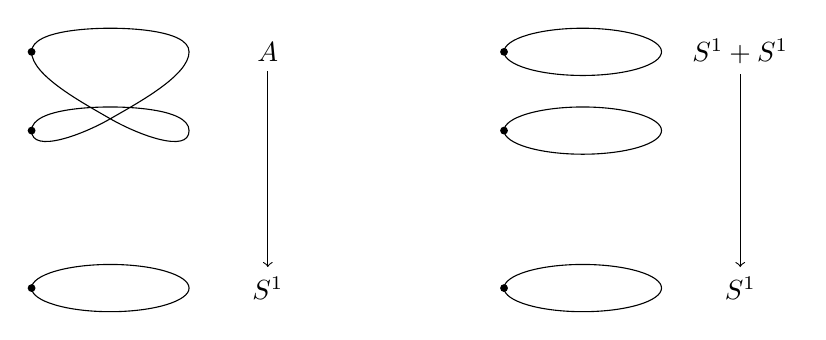
\begin{tikzpicture}
    \node (A) at (2,1) {$A$};
    \node (B) at (2,-2) {$S^1$};
    \draw[->] (A) -- node[auto] {$$} (B);
    \draw (0,-2) ellipse (1 and .3);
    \draw (-1,0)
    .. controls ++( 90:-.3) and ++(210: .4) .. (0,0.15)
    .. controls ++(210:-.4) and ++(270: .3) .. (1,1)
    .. controls ++(270:-.3) and ++(  0: .1) .. (0,1.3)
    .. controls ++(  0:-.1) and ++( 90: .3) .. (-1,1)
    .. controls ++( 90:-.3) and ++(150: .4) .. (0,0.15)
    .. controls ++(150:-.4) and ++(270: .3) .. (1,0)
    .. controls ++(270:-.3) and ++(  0: .1) .. (0,0.3)
    .. controls ++(  0:-.1) and ++( 90: .3) .. (-1,0);
    \node[fill,circle,inner sep=1pt] at (-1,-2) {};
    \node[fill,circle,inner sep=1pt] at (-1,0) {};
    \node[fill,circle,inner sep=1pt] at (-1,1) {};
%    \node (L) at (1,-3) {(left)};
    \begin{scope}[xshift=6cm]
    \node (At) at (2,1) {$S^1+S^1$};
    \node (Bt) at (2,-2) {$S^1$};
    \draw[->] (At) -- node[auto] {$$} (Bt);
    \draw (0,-2) ellipse (1 and .3);
    \draw (0,0) ellipse (1 and .3);
    \draw (0,1) ellipse (1 and .3);
    \node[fill,circle,inner sep=1pt] at (-1,-2) {};
    \node[fill,circle,inner sep=1pt] at (-1,0) {};
    \node[fill,circle,inner sep=1pt] at (-1,1) {};
%    \node (Lt) at (1,-3) {(right)};
    \end{scope}
  \end{tikzpicture}
  \caption{A visualization of two \coverings over the circle}
  \label{fig:covering}
\end{figure}

\begin{remark}
  It \emph{is} possible to misunderstand what a ``connected \covering'' is: 
the other interpretation ``all the preimages are connected'' simply 
would give us an equivalence (since connected sets are contractible),
and this is \emph{not} what is intended. (Equivalences are \coverings, but not necessarily connected \coverings and connected \coverings are not neccesarily equivalences.)  

Likewise, for the other qualifications; for instance in a ``finite covering'' $f:A\to B$, the type $A$ is usually \emph{not} a finite set. 

  We trust the reader to keep our definitions in mind and not the other interpretations.
\end{remark}


\begin{remark}
  \Coverings are closely related to a concept from topology called ``covering space'' (or any variant thereof, including Galois theory) and from algebra as sheaves (of sets).  Either way, the concept is useful because it singles out the (sub)symmetries.  
\end{remark}

% \begin{remark} MB: HAS BEEN MOVED TO A PLACE WHERE IT IS DIRECTLY USED
%\label{rem:setfamloopinj}
% We recall \cref{cor:fib-vs-path} stating that all the fibers of a map $f:A\to B$ 
% are sets if and only if each  $$\ap{f}: (a=a')\to (f(a)=f(a'))$$ is an injection.
%\end{remark}

% \begin{definition}\label{def:decktrafo}\footnote{postpone}
%   Let $f:A\to B$ be a \covering.  A symmetry $(A,f,!)=(A,f,!)$ is called a \emph{deck transformation}.
% \end{definition}
%specified by a pair $(p_A,p_f)$ with consisting of a $p_A:A=_{\UU}A'$, a $p_f:f'p_A=_{A\to B}f$.

\begin{example}\label{xca:coveringsofS1}
Let us consider \coverings over the circle, most conveniently 
for the moment in the guise of families 
$$E:\Sc\to\Set.$$
By circle induction, giving such an $E$ is the same as 
specifying a set $E(\base)$ and a symmetry $E(\Sloop):E(\base)=E(\base)$.  
Said more concisely in terms of \cref{lem:freeloopspace}, 
the type of \coverings over the circle is equivalent to 
$$\sum_{X:\Set}(X=X).$$ \footnote{\color{blue}%
DUPLICATE, BETTER LATER
We will ultimately show that the circle $\Sc$ is equivalent to the 
component (see \cref{def:connected}) $C$ of $(\zet,\etop{s})$ in $\sum_{X:\Set}(X=X)$,  
where $s:\zet\to\zet$ is the successor.  This may seem circular: ``the circle is equivalent to a component of the type of \coverings over the circle!'' 
(MB WHY CIRCULAR: $\sum_{X:\Set}(X=X)$ EXISTS ALSO INDEP OF CIRCLE?)
but it really just condenses the idea that connected groupoids are uniquely 
given by their symmetries.}
\end{example}
A particularly important example is the following:
\begin{definition}\label{def:RtoS1}
Define $R:\Sc\to\UU$ by circle induction by setting 
$R(\base)\defeq\zet$ and $R(\Sloop)\defis \etop{s}$.
Since $\zet$ is a set, and being a set is a proposition,
one can prove by circle induction that $R(z)$ is a set for all $z:\Sc$.
(Abusing notation we also write $R:\Sc\to\Set$.) Now define
$$\RR\defeq\sum_{z:\Sc}R(z)$$
and let the first projection denoted by
$$\exp:\RR\to \Sc$$
be the \emph{exponential \covering of the circle}.
\end{definition}

\begin{remark}
  \label{rem:expforreal}
  The reason for the name $\exp:\RR\to \Sc$ comes from the following visualization.  
%Consider the real and complex numbers $\RR$ and $\mathbb C$.  
If $x$ is a real number, then the complex exponentiation 
$e^{2\pi i x}=\cos(2\pi x)+i\sin(2\pi x)$ has absolute value $1$ and 
so defines a continuous function from the real numbers to the unit circle.  
Choosing any point $z$ on the unit circle, we see that the preimage of $z$ under the exponential function is a shifted copy of the integers inside the reals. 
 
This connection between the integers and the unit circle is precisely captured in a form that we can take further by the \covering $\exp:\RR\to \Sc$.
\end{remark}

We already defined a \covering $f:A\to B$ to be universal if $A$ is connected
and all $a=_A a$ (for $a:A$) are connected. 
If moreover $B$ is a pointed, connected groupoid we shall argue that
we actually can speak of \emph{the} universal \covering.

Recall \cref{cor:fib-vs-path} stating that all the fibers of a map $f:A\to B$ 
are sets if and only if each 
\[
\ap{f}: (a=a')\to (f(a)=f(a'))
\]
is an injection. Assume $B$ is a groupoid.
We prove that $A$ is contractible. 
Being contractible is a proposition, so we may assume 
we have an element $a$ of $A$ since $A$ is connected. 
By \cref{xca:connected-trivia} and \ref{xca:component-connected} 
it suffices to prove that $a=a$ is contractible.
By \cref{xca:prop-set-trivia}, using that $a=a$ is connected,
it suffices to show that $a=a$ is a set.
Using that $\ap{f}$ is an injection, we can apply the remark after
\cref{lem:sum-of-fibers} and obtain that $a=a$ is a set since
$f(a)=f(a)$ is a set, since $B$ is a groupoid.
This completes the proof that $A$ is contractible.

Now assume $(B,b_0)$ is a pointed connected groupoid and $f:A\to B$
a universal \covering. We first prove the proposition $\Trunc{f^{-1}(b_0)}$.
In doing so we may assume an element of $A$. Since $B$ is connected
we have $\Trunc{b_0 = f(a)}$. Again we may assume an element $p: b_0=f(a)$.
Thus $\trunc{(a,p)}:\Trunc{f^{-1}(b_0)}$. 
We can now replay the above argument that $A$ is contractible starting
with a pair $(a,p)$ in $f^{-1}(b_0)$, so that $p: b_0 = f(a)$.
Note that, since $A$ is contractible and $B$ is a groupoid,
$f^{-1}(b)$ is equivalent to the set $b_0 = b$.
This leads to the following definition.\footnote{%
If $B$ is a pointed connected groupoid,
\emph{any} universal \covering is merely equal to \emph{the} universal \covering.
This should be good enough.}

\begin{definition}
  \label{def:universalcover}
  Let $(B,b_0)$ be a pointed connected groupoid.  
The \emph{universal \covering}\footnote{for $B$ not a groupoid this is total misuse of language.  I feel sort of bad about it, but I did not want to say ``path fibration''} of $B$ is the \covering of $B$ given by the family of sets 
  $$\uc{b_0}:B\to\Set,\quad \uc{b_0}(b)\defequi (b_0=_Bb),$$
or alternatively as the first projection from $\uc{b_0}B\defequi\sum_{b:B}(b_0=_Bb)$ to $B$. 
\end{definition}
Note that $(b_0=_B b)$ is a family of \emph{sets} exactly when $B$ is a groupoid. 
However, we have \cref{lem:thepathspaceiscontractible} for any type $B$.

\begin{remark}
  What's so ``universal'' about this?
  %This seems to deflates the concept ``universal \covering'' of a pointed connected groupoid $(B,b_0)$, since we've just shown that t
The universal \covering over the pointed connected groupoid $(B,b_0)$ coincides with the constant function $c_{b_0}:\bn 1\to B$ (with value $b_0$), and seems like an unnecessary complicated representation were it not for the manifold practical value of the formulation that we've given.  
In particular, we recognize the set of symmetries $b_0=_Bb_0$ as the preimage of $b_0$ under the first projection from $\uc{b_0}B$ to $B$; ultimately this will show that the study of symmetries coincides with the study of the universal \covering.

The first instance of this comes already in the next section, where we show in \cref{cor:S1groupoid} that the symmetries of the circle is given by the set of integers $\zet$ by showing that the universal \covering and the exponential \covering (\cref{def:RtoS1}) of the circle coincide.

That said, one way to see that the constant function $c_{b_0}:\bn 1\to B$, \emph{does} deserve the label universal because if given any function $f:A\to B$ and an $(a_0,p): f^{-1}(b_0)$, then we get a function $c_{a_0}:\bn 1\to A$ and $p:b_0=f(a_0)$ gives an element in $c_{b_0}=_{\bn 1\to B}f\, c_{a_0}$.  In other words, any such $f$ is ``a factor of $c_{b_0}$''.  
Note, however, that this depends on $f^{-1}(b_0)$ being non-empty (classically, this is often demanded of a covering, which distinguishes it from our \coverings), and the factorization depends on the element $(a_0,p)$ used. 
\end{remark}



\section{The symmetries of the circle}
\label{sec:pi1S1isZ}\label{sec:symcirc}

With the set $\zet$ of integers \emph{defined} as in \cref{sec:integers}, 
we will now \emph{prove} that $\zet$ is equivalent to the type 
$\base=_{\Sc}\base$, and that under this equivalence $0:\zet$ corresponds to 
$\refl{\base}:\base=\base$, and $1$ to $\Sloop$, and $-1$ to $\Sloop^{-1}$. 
More generally, the successor $\etop{s}:\zet=\zet$ corresponds to composition with $\Sloop$
and the predecessor corresponds to composition with $\Sloop^{-1}$.

The first step is to prove that the exponential \covering \cref{def:RtoS1} 
is equal to the universal \covering in \cref{def:universalcover}, 
\ie we prove that the family 
\[
R: \Sc\to\UU,\qquad R(\base)\defeq\zet,\, R(\Sloop)\defis \etop{s}
\]
is equal to the family
\[
\uc{\base}:\Sc\to\UU,\qquad \uc{\base}(z)\defeq (\base=z).
\]
What does it mean for the families $\uc{\base}$ and $R$ to be equal?
Type families are a special case of functions. 
Function extensionality reduces the question to pointwise equality
of $\uc{\base}$ and $R$ as functions.
Using univalence, it suffices to give
an equivalence from $\uc{\base}(z)$ to $R(z)$, for every $z:\Sc$.

%We define two functions, $f:\uc{\base}\to R$ and $g:R\to \uc{\base}$ and show that, 
% under univalence, they define inverse identities.  

We first recall from \cref{sec:heavy-transport} how 
transport behaves in families of function types.  
Given a type $A$ and two type families $P,Q:A\to\UU$, 
%$P\to Q$ is shorthand for the type $(P\to Q) \jdeq \prod_{a:A}(P(a)\to Q(a)$.  
transport along $p:a=_Aa'$ of $f:P(a)\to Q(a)$ is $Q(p)\,f\,P(p)^{-1}:P(a')=Q(a')$.
In a picture
\[
\xymatrix{
P(a)\ar[rr]^{f}\ar@{=}[d]^{P(p)}_\downarrow&&
  Q(a)\ar@{=}[d]^{Q(p)}_\downarrow\\
P(a')&&\,Q(a').}
\]
If $A$ is $\Sc$, then the induction principle for the circle says 
that giving an $f(z):P(z)\to Q(z)$ for all $z:\Sc$ is the same as 
specifying an $f(\base):P(\base)=Q(\base)$ and an identity 
$f(\Sloop):Q(\Sloop)\,f(\base)\,P(\Sloop)^{-1}=_{P(\base)\to Q(\base)}f(\base)$,
\ie a witness that the composites in 
$$\xymatrix{
  P(\base)\ar[rr]^{f(\base)}\ar@{=}[d]^{P(\Sloop)}_\downarrow
 &&Q(\base)\ar@{=}[d]^{Q(\Sloop)}_\downarrow\\
  P(\base)\ar[rr]^{f(\base)}&&\,Q(\base)}
$$
are equal.  If $P,Q$ are families of sets, 
then the type of $f(\Sloop)$ is a proposition.

We now define two fiberwise maps that will turn out to give
inverse equivalences between $\uc{\base}(z)$ and $R(z)$, for each $z:\Sc$.

\begin{definition}
  \label{def:fPtoR}
  The function $f:\prod_{z:\Sc}(\uc{\base}(z)\to R(z))$ is defined by transport: $f(z)(p)\defequi\trp{R,p}(0)$.
\end{definition}

In Figure~\ref{fig:transportalongloop}, the transport in the definition
above has been visualised for $p={\Sloop^n}$, $n=-2,-1,0,1,2$.

\begin{figure}[h]
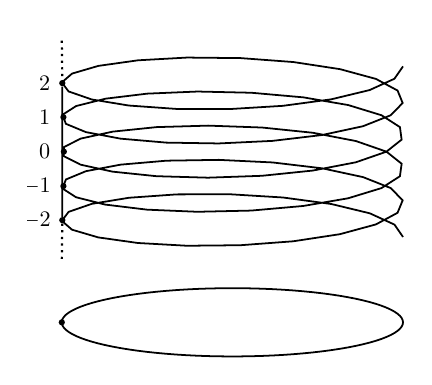
\begin{tikzpicture}[scale=0.8]
\begin{axis}[axis lines=none,line width=1pt, axis equal image]

\node at (-10,13) () {$\zet$}; %CUTOFF FOR UNKNOWN REASON
\node [] at (-10,12) (A) {};

\addplot[domain=0:10*pi,samples=100,black,no marks,thick] %500 samples slow
({10*cos(deg(x))}, % x-coordinate
{2*sin(deg(x)) + x/pi}) % y-coordinate
node [circle,scale=0.3,fill,pos=0.9] (B) {} % point (A)
node [circle,scale=0.3,fill,pos=0.7] {} % point (A)
node [circle,scale=0.3,fill,pos=0.5] {} %
node [circle,scale=0.3,fill,pos=0.3] {} % 
node [circle,scale=0.3,fill,pos=0.1] (C) {}; %

\node at (-11,9) () {$2$};
\node at (-11,7) () {$1$};
\node at (-11,5) () {$0$};
\node at (-11,3) () {$-1\;\;\,$};
\node at (-11,1) () {$-2\;\;\,$};

\node [] at (-10,-2) (D) {};
\node at (0,-5) () {$\Sc$};
\node at (9,-5) () {$\Sloop$};

\addplot[domain=0:2*pi,samples=100,black,no marks,thick] %500 samples slow
({10*cos(deg(x))}, % x-coordinate
{2*sin(deg(x))-5}) % y-coordinate
node [circle,scale=0.3,fill,pos=0.5] (E) {}; % point (D)


\draw[dotted] (A)--(B);
\draw[thick] (B)--(C);
\draw[dotted] (C)--(D);

\end{axis}
\end{tikzpicture}
\caption{Transport in the family $R$}
\label{fig:transportalongloop}
\end{figure}

\begin{lemma}\label{lem:windingnumber}
For $f$ as in \cref{def:fPtoR} we have $f(\base)(\Sloop^n)=n$ for all $n:\zet$.
\end{lemma}
\begin{proof}
By induction on $n:\zet$.  In the base case $n=0$ we have
$f(\base)(\Sloop^0)\defeq f(\refl\base)\defeq 0$.
For $n=s(m)$ with $m:\NN$ we have\footnote{some references needed here} 
\begin{align*}
  f(\base)(\Sloop^{s(m)})&\defeq\trp{R,\Sloop^{s(m)}}(0)\\
  &=\trp{R,\Sloop \Sloop^{m}}(0)\\
  &=\trp{R,\Sloop}(\trp{R,\Sloop^m}(0))\\
  &=s(\trp{R,\Sloop^m}(0)).
\end{align*}
The last equality follows from $\etop{s}=R(\Sloop)$ using
$s=\cast(\ua(s))=\cast(\etop{s})=\trp{\id_\UU,\etop{s}}=\trp{R,\Sloop}$, 
see \cref{def:idtoeq} and \cref{def:univalence}.
For negative $n$ the proof is similar.
\end{proof}

In the definition of the second map, 
take into account that $R(\base)\jdeq \zet$ and $\uc{\base}(\base) \jdeq (\base=\base)$.

\begin{definition}\label{def:gRtoP}
The function $g:\prod_{z:\Sc}(R(z)\to \uc{\base}(z))$ is 
defined by circle induction: 
\[
g(\base)\defeq {\Sloop^{-}}:\zet\to(\base=\base) : n \mapsto {\Sloop^n}
\]
and 
\[
g(\Sloop): \uc{\base}(\Sloop)\, g(\base)\,R(\Sloop)^{-1}=_{\zet\to (\base=\base)} g(\base).
\]
So far we have only given the type of $g(\Sloop)$. By definition, $R(\Sloop)$ is $s$
and $\uc{\base}(\Sloop)$ is composition with $\Sloop$.
In a picture, $g(\Sloop)$ should prove that it does not matter what 
path you take around the square
$$\xymatrix{\zet\ar[rr]^{\Sloop^-}\ar@{=}[d]^s_\downarrow
 &&(\base=\base)\ar@{=}[d]^{\Sloop\cdot\_}_\downarrow\\
  \zet\ar[rr]^{\Sloop^-}&&\,(\base=\base).}
$$
This follows by a simple calculation: ${\Sloop\,\Sloop^{n-1}} = {\Sloop^n}$, 
for all $n:\zet$. 
\end{definition}


\begin{lemma}
  \label{lem:univisexp}
For every $z:\Sc$, the functions $f(z)$ defined in \cref{def:fPtoR} 
and $g(z)$ in \cref{def:gRtoP} are inverse equivalences between
$\uc{\base}(z)$ and $R(z)$.
%$\uc{\base}$ defines a connected \covering of the circle: $\uc{\base}(z)\defeq (\base=z)$ is a set for all $z:\Sc$ and the type $\uc{\base} \Sc$ is connected (more precisely, by univalence $\uc{\base}(z)$ is equal to the set $R(z)$ and $\uc{\base} \Sc$ is contractible).
\end{lemma}
\begin{proof}
We apply \cref{lem:weq-iso} and verify the two conditions.
  Firstly, we need to give elements $H(z,p):g(z)(f(z)(p))=p$
for all $z:\Sc$ and $p:\uc{\base}(z)\defeq(\base=z)$. 
By induction on $z$ and $p:\base=z$ it suffices to set 
$H(\base,\refl\base)\defeq\refl{\refl{\base}}$ since
$g(\base)(f(\base)(\refl{\base}))\jdeq g(\base)(0)\jdeq\refl{\base}$.

Secondly, we need to give elements $G(z)(n):f(z)\,g(z)(n))=n$
for all $z:\Sc$ and $n: R(z)$.
By circle induction it suffices to define $G(\base)$ and $G(\Sloop)$,
but since $\zet$ is a set the information for $G(\Sloop)$ is redundant.
Hence, we need to show that for all $n:\zet$ that 
$f(\base)(g(\base)(n))\jdeq  f(\base)(\Sloop^n)$ is equal to $n$.  
This follows from \cref{lem:windingnumber}. 
\end{proof}


\begin{corollary}\label{cor:S1groupoid}
The circle $\Sc$ is a groupoid, and the function
%$\uc{\base}$ is a \covering, NOT NEEDED
\[
{\Sloop}^{-} : \zet\to(\base=_{\Sc}\base) %\text{sending $n$ to ${\Sloop}^n$}
\]
sending $n$ to $\Sloop^n$ is an equivalence.
\end{corollary}
\begin{proof}
For any $z:\Sc$, the type $\uc{\base}(z)\jdeq (base=_{\Sc}z)$ is a set 
since $R(z)$ is a set and $\uc{\base}(z) \equiv R(z)$.
Since the circle is connected and being a set is a proposition, it follows
that $y=_{\Sc}z$ is a set, for any $y,z:\Sc$. Hence $\Sc$ is a groupoid.
By \cref{def:gRtoP}, ${\Sloop}^{-}\jdeq g(\base)$ is an equivalence.
\end{proof}


\section{A reinterpretation of the circle}
% and a criterion for equivalence through \coverings}
\label{sec:S1isC}
In this section we return to the considerations discussed in \cref{xca:coveringsofS1}.
Through \cref{lem:freeloopspace} we can get a different perspective on the circle which highlights it as a type classifying very simple symmetries.
By \cref{lem:freeloopspace} (moving up one universe), a type family $\Sc\to\UU$ is uniquely given by a type $X:\UU$ together with a $i:X=_\UU X$, with no further requirements on $i$.
Using UA, any type $X$ and any equivalence $f: X\equiv X$ provides such a pair
$(X,\etop{f})$. We have seen one example in \cref{def:RtoS1}, 
namely the set $\zet$ of integers together with the successor $s: \zet\equiv\zet$.

The importance of the latter example will become apparent when we eventually 
explain that \emph{the circle is equivalent to the connected component of 
$(\zet,\etop{s})$ in the type $\sum_{X:\UU}(X=_{\UU}X)$}. 

Heading towards this goal, we investigate this component a bit further.
Define the type family $D$ by $D(X) \defeq (X=X)$ for all $X:\UU$.
Recall from \cref{lem:isEq-pair=} that, given $X:\UU$ and $i: X=X$, 
the identity type $(\zet,\etop{s}) = (X,i)$
is equivalent to the type of pairs consisting of a $p:\zet=X$ and 
a proof of $\pathover{\etop{s}}{D}{p}{i}$. The latter type is
equivalent to $\trp{D,p}(\etop{s}) = i$ by \cref{def:pathover-trp}.
The transport is by conjugation,
\cref{xca:trp-in-a/x=b/x}(\ref{trp-in-x=x}), so that the latter
type is equivalent to $p\cdot\etop{s}\cdot p^{-1} = i$, 
and to $p\cdot\etop{s} = i\cdot p$, or $p \etop{s} = i p$ for short. 
In total, the identity type $(\zet,\etop{s})=(X,i)$ is equivalent to
\[
\sum_{p: {\zet = X}} {p \etop{s}} =_{\zet=X} {i p}.
\] 
Since $\zet$ is a set, this sum type is a set.
In particular, the type of symmetries $(\zet,\etop{s})=(\zet,\etop{s})$
is equivalent to the set $\sum_{p:\zet=\zet}p\etop{s}=\etop{s}p$.  

% and so our component $C$ is a connected groupoid. LATER FROM C=S1

This discussion tells us that the following definition makes sense:

\begin{definition}\label{def:S1toC}
Let $C$ be the component of $\sum_{X:\UU}(X=_{\UU}X)$ containing $(\zet,\etop{s})$.
Define by circle induction
\[
c:\Sc\to C \text{~setting~} 
c(\base)\defequi (\zet,\etop{s},\trunc{\refl{(\zet,\etop{s})}})
\]
and $c(\Sloop): c(\base)=_C c(\base)$ given by the successor 
$\etop{s}:\zet=\zet$ and trivial proofs of the proposition
$\etop{s}\etop{s}=\etop{s}\etop{s}$ and the proposition for the 
truncated third component of $c(\base)$.
\end{definition}

We will henceforth leave out the third component from the denotation
of elements of $C$, since its type is propositional and does not convey 
any information beyond its mere existence. We may write a ``!'' in order
to remind the reader of hidden information of propositional type.
  
We start by identifying the symmetries of $(\zet,\etop{s})$ in $C$:

\begin{lemma}
  \label{lem:IdCisZet}
Any element in $(\zet,\etop{s})=_C(\zet,\etop{s})$ is of 
the form $\pathpair{\etop{s}^k}{!}$ for some unique $k:\zet$.  
In other words, the function 
\[
\ev_0:((\zet,\etop{s})=_C(\zet,\etop{s}))\to \zet 
\text{~defined by~} \ev_0(\pathpair{p}{!}) \defeq \ptoe{p}(0)
\]
is an equivalence.
\end{lemma}
\begin{proof}
  Given $\pathpair{p}{!}:(\zet,\etop{s})=_C(\zet,\etop{s})$ we must determine 
$p:\zet=\zet$. By univalence this amounts to giving all the values 
$\ptoe{p}(n)$ for $n:\zet$.  However, since $s\ptoe{p}=\ptoe{p}s$ we 
get that $\ptoe{p}(n+1)=\ptoe{p}(n)+1$ for all $n:\zet$. 
Induction on $n:\zet$ (positive and negative $n$ separately) gives that 
$\ptoe{p}(n)=n+\ptoe{p}(0)$. Hence $\ptoe{p}=s^{\ptoe(0)}$, so $p=\etop{s}^k$
for some unique $k:\zet$.
\end{proof}

We are going to prove that $c$ is an equivalence.
The method of proof will be used on several occasions.
Therefore we isolate the following general result first.

\begin{lemma}\label{lem:conn-eq-f-ap-f-x}
Let $X$ and $Y$ be connected types, $x$ an element of $X$,
and $f$ a function from $X$ to $Y$. Then $f$ is an equivalence
if and only if $\ap{f}: (x=x) \to (f(x)=f(x))$ is an equivalence.
\end{lemma} 
\begin{proof}
Using \cref{cor:fib-vs-path}(\ref{conn-fib-vs-path}) it suffices to show that 
each $\ap{f}$ is an equivalence if and only if the specific $\ap{f}$ with 
domain $x=x$ is an equivalence. Being an equivalence is a proposition, 
so this follows in two easy steps from $X$ being connected,
using \cref{xca:component-connected}.
\end{proof}

\begin{theorem}\label{thm:S1bysymmetries}
  The function $c:\Sc\to C$ from \cref{def:S1toC} is an equivalence.
\end{theorem}
\begin{proof}
  In view of \cref{lem:conn-eq-f-ap-f-x} we only need to show that 
$\ap{c}:(\base=_{\Sc}\base)\to((\zet,s)=_C(\zet,s))$ is an equivalence.
\footnote{ ((can we call equivalences between sets bijections?)). YES, BUT NOT NEEDED}
Note that both the domain and the co-domain of $\ap{c}$ is equivalent to $\zet$.
Consider the following diagram in which we compose $c$ with the equivalences
from \cref{cor:S1groupoid} and \cref{lem:IdCisZet}:
\[
\xymatrix{
\zet\ar[rr]^-{\Sloop^{{-}}}&&
(\base=\base)\ar[rr]^-{\ap{c}}&&
((\zet,s)=_C(\zet,s))\ar[rr]^-{\ev_0}&&
\zet}
\]
For $c$ to be an equivalence, it suffices to show that the composition
is the identity on $\zet$. By definition $\ap{c}(\Sloop) = \pathpair{\etop{s}}{!}$, 
and by induction on $n:\zet$
one shows  $\ev_0(\ap{c}(\Sloop^n))=\ev_0(\pathpair{\etop{s}^n}{!}) = s^n(0) = n$. 
% The composition with the functions $\Sloop^-:\zet\to (\base=_{\Sc}\base)$ sending $n:\zet$ to $\Sloop^n$ and $\ev_0:((\zet,s)=_C(zet,s))\to \zet$ of \cref{lem:IdCisZet} given by $\ev_0(p)=p(0)$ gives us a function $w:\zet\to\zet$ with $w(n)=s^n(0)$.  From \cref{cor:S1groupoid} we know that $\Sloop^-$ is an equivalence, so we only need to show that $w$ is an equivalence
\footnote{I may have used 2-out-of-3 before, we probably need to include it somewhere, though by univalence it hardly seems necessary}% .  If $p:\zet=\zet$ with $!:sp=ps$, we get by induction on $n:\zet$ (induction for positive and negative $n$ separately) that $p(n)=n+p(0)$.  Hence, all the elements in the preimage $w^{-1}(p,!:sp=ps)$ are equal to $(p(0),!)$.  
\end{proof}

% Now, consider the function 
% $$f:\sum_{p:\zet=\zet}(sp=ps)\to\zet,\qquad f(p,!)=p(0).$$  If $a:\zet$, then $f^{-1}(a)$ consists of the $p:\zet=\zet$ with $sp=ps$ and $p(0)=a$ (the last two are propositions), but by induction we see that $p(n)=n+a$ for all $n:\zet$ (separate induction on positive and negative numbers).  In other words, all elements in the set $f^{-1}(a)$ are equal, and so $f$ is an equivalence


%   ((TODO))
% As an illustration of things to come in a simpler setting, we can give the torsor definition of the circle, where Marc makes the simplifying observation that (since the integers is free on one generator) this can be coded in terms of the successor and there is a priori no need to talk about the abstract group.  In short: an (abstract) $\ZZ$-set is uniquely given by a set $X$ with an identity $f: X=_{\Set}X$.  A $\ZZ$-torsor $(X,f)$ is a $\ZZ$-set (merely) equal to $(\zet,S)$ ($S$ is the successor), that, there is a $p:X=\zet$, so that $Sp=_{X=X} pf$.  This is based at (the pricipal $\ZZ$-torsor represented by) $(\zet,S)$ and $(\zet,S)=(\zet,S)$ consists of $f:\zet=\zet$ s.t. $Sf=fS$.  Such an $f$ must be given by addition by the integer $f(0)$.  This gives us an equivalence between $\Sc$ and the type of (secret) $\ZZ$-torsors.  This will be trivial if we have shown that a map of connected groupoids is an equivalence if it induces an equivalence on the identity sets.

\section{Other \coverings over the circle}
\label{sec:covS1}

Let $A$ be a type and $f:A\to \Sc$ a function.
By \cref{cor:fib-vs-path}(\ref{set-fib-vs-path}), $f$ is a \covering
over $\Sc$ if and only if each $\ap{f}$ is injective.
Assume that $f:A\to \Sc$ is a \covering with $A$ is connected.
Let $(a_0,p)$ be an element of $f^{-1}(\base)$. 
By \cref{xca:component-connected}
the condition that \emph{each} $\ap{f}$ is injective
can be relaxed to $\ap{f}: (a_0=a_0)\to(f(a_0)=f(a_0))$ being injective.
Now look at the following subset:
\[
\set{~ l: \base = \base \mid {\ap{f}}^{-1}(plp^{-1})~ }.
\]
Clearly, a classification of connected \coverings over the circle
also classifies certain subsets of symmetries of $\base$.
Such subsets are closed under concatenation and inverses,
since $\ap{f}$ is compatible with these operations,
see \cref{lem:apcomp}.
Using language yet to be introduced, we actually ``classify the subgroups of the integers''.

We start by giving some examples of connected \coverings of the circle.
In the course of our discussion, we will see that -- assuming a weak form
of the Law of the Excluded Middle -- these are all the decidable connected 
\coverings over the circle.

\begin{example}\label{exa:univS1cover}
The \emph{universal} \covering from \cref{def:universalcover}
is the map $c_\base:\bn 1\to \Sc$ 
sending the unique element of $\bn 1$ to $\base$. 
(It takes this simple form since the circle is a pointed connected
groupoid, see the discussion before \cref{def:universalcover}.)
The universal \covering corresponds to the subset consisting 
of $\refl\base : \base=\base$ only.  
\end{example}

\begin{example}\label{exa:mfoldS1cover}
For $m:\NN$ positive, define the \emph{degree $m$ function} by circle induction
\[
-^m:\Sc\to \Sc, \text{~~setting~} 
-^m(\base)\defeq\base \text{~~and~} 
-^m(\Sloop)\defis{\Sloop}^m.
\]
This \covering corresponds to the subset consisting 
of ${\Sloop}^{mn} : \base=\base$ for all $n:\zet$.
\end{example}

Note that the degree $0$ function would be constant,
and hence not a \covering since the domain is not a set,
see \cref{xca:constant-cover}

\begin{remark}
  \label{rem:RtoS1}
The universal \covering is essentially the same as defined in \cref{def:RtoS1}
and explained in \cref{rem:expforreal}
since the real numbers form a contractible space.

\label{rem:finitecoveringsofS1}
The analogue of our degree $m$ function is the $m$-th power of complex numbers 
restricted to the unit circle. % mapping $z$ to $z^m$ if $|z|=1$.  
The following visualization is perhaps more tangible.  
Let $m=12$ and picture the circle and mark $12$ evenly spaced points.
This will look like a clock, with marks $1,2,\dots,12$. 
You can then make a function from the circle to itself by sending 
all marks to $12$ and each of the arcs connecting the marks to the entire circle 
-- (in a continuous manner preserving the orientation).
  ((picture!!))
\end{remark}

We could be more ambitious and ask: what is the \emph{type} of decidable 
\coverings over the circle?  Since the type of \coverings is 
equivalent to $\Sc\to \Set$, and $\Set$ is a groupoid
(\cref{lem:Set-is-groupoid}),
\cref{lem:level-n-utils}(\ref{level-n-utils-codom}) gives
that the type of decidable \coverings over the circle is a groupoid.  
We will pin this groupoid down by first identifying the components 
(of which there turns out to be one for each natural number), 
and then analyzing one component at a time.

Recall the function $c:\Sc\to C$ of \cref{def:S1toC}. 
By \cref{thm:S1bysymmetries} we know that $c$ is an equivalence, 
so classifying \coverings over $\Sc$ is equivalent to 
classifying \coverings over $C$.  
We simplify the notation slightly, letting $\pt_C\defeq(\zet,\etop{s}):C$ 
(so that $\pt_C \jdeq c(\base)$ with $c$ from \cref{def:S1toC}), 
and allowing ourselves to write $s:\pt_C=_C\pt_C$ instead of the 
more honest $\pathpair{\etop{s}}{!}:\pt_C=_C\pt_C$ 
(equal to the $c$-image of ${\Sloop}:\base=\base$).

It is instructive to rephrase the examples of connected \coverings over $\Sc$ in 
terms of $C$, even though they could be transported along the identity $\bar c:S^1=C$ corresponding to $c$.

\begin{example}\label{exa:univCcover}
The universal \covering is represented by the constant function
$c_{(\zet,\etop{s})}:\bn 1\to C$ sending the unique element 
of $\bn 1$ to $(\zet,\etop{s}):C$.
\end{example}

\begin{example}\label{exa:mfoldCcover}
Assume that $m:\NN$ is positive.  We now give a description of 
the $m$-fold \covering over the circle in terms of $C$.

We proceed as follows.  First we presenting the answer, a covering we call $-^m:C\to C$ and then we prove that $-^m:S^1\to S^1$ and $-^m:C\to C$ the  correspond to each other under the equivalence $c:S^1\we C$. 

 What should we require of $-^m(X,f)$ for $(X,f):C$? Well, $-^m:S^1\to S^1$ sends $\base$ to $\base$ and $\Sloop$ to $\Sloop^m$; somehow only the $\Sloop^k$ where $k$ is a multiple of $k$ is in the image of $-^m$.  So we have to find an element $(Y,r):C$ with ``$r^m$ corresponding to $f$''.  We achieve this by ``streching'' $X$: let $Y$ be $m$ copies of $X$ and let $r$ jump idly from one copy to another except every $m$th time when $r$ also is allowed to use $f$.  
This is illustrated in \cref{fig:root} with the shift by $f$ being 
vertical and the movement from copy to copy going around a circle.  
\begin{figure}[bt]
  \centering
  \begin{tikzpicture}
    \node (A) at (4,1) {\quad$\sqrt[m]f:{\bn m\times X}\to{\bn m\times X}$};
    \foreach \y in {0,1,2}
    { \begin{scope}[shift={(0,\y)}]
        \foreach \x in {0,...,4}
        { \node[fill,circle,inner sep=1pt] at (180+72*\x:1 and .3) {}; }
        \foreach \x in {0,...,3}
        { \draw[-stealth] (180+72*\x:1 and .3) arc(180+72*\x:252+72*\x:1 and .3); }
      \end{scope} }
    \foreach \y in {1,2}
    { \begin{scope}[shift={(0,\y)}]
        \draw[-stealth] (108:1 and .3)
        .. controls ++( 5:-.3) and ++(80:.2) .. (-.7,-.4)
        .. controls ++(80:-.2) and ++(90:.2) .. (-1,-1);
      \end{scope} }
    \draw[-stealth] (108:1 and .3)
    .. controls ++( 5:-.3) and ++(80:.2) .. (-.7,-.4);
    \node (dz) at (-.7,-.7) {\footnotesize$\vdots$};
    \begin{scope}[shift={(0,3)}]
      \draw[-stealth] (-.7,-.4)
      .. controls ++(80:-.2) and ++(90:.2) .. (-1,-1);
      \node (da) at (-.7,0) {\footnotesize$\vdots$};
    \end{scope}
    \draw [decorate,decoration={brace,amplitude=10pt}]
    (-1.1,-.8) -- (-1.1,2.8) node [black,midway,xshift=-20pt] {\footnotesize $X$};
    \draw [decorate,decoration={brace,amplitude=10pt}]
    (1,-1) -- (-1,-1) node [black,midway,yshift=-15pt] {\footnotesize $\bn{m}$};
  \end{tikzpicture}
  \caption{The $m$-th root of a function $f: X\to X$}
  \label{fig:root}
\end{figure}

% First,
% for $\Sc$ we have $-^m(\base)\jdeq\base$.    and for $C$, as we
% will see, we get $(\zet,\etop{s}) = -^m(\zet,\etop{s})$, 
% with $=$ and not with $\jdeq$.
% Let's say $-^m(\zet,\etop{s})\jdeq(Y,\etop{r})$.
% The loop of $(\zet,\etop{s})$ is based on $s$,
% the corresponding loop of $(Y,\etop{r})$ is based on $r$.
% The challenge is to arrange things in such a way that
% $-^m$ acting on $s$ yields $r^m$.
% This motivates the following definition.

More precisely, for any type $X$ and $f:X\to X$, we define the $m$-th \emph{root}
\[
{\sqrt[m]f} : {\bn m\times X} \to {\bn m\times X}
\]
of $f$ by setting 
\[
\sqrt[m]f(i,x)\defeq
\begin{cases}
  (i+1,x)& \text{for $i<m-1$ and}\\
  (0,f(x))& \text{for $i=m-1$}.
\end{cases}
\] 
Only one $m$-th of the time does $\sqrt[m]f$ use $f:X\to X$,
the rest of the time it increases the element in $\bn m$).
Indeed, iterating $\sqrt[m]f$ we get $(\sqrt[m]f)^m(i,x)=(i,f(x))$; 
hence the term ``$m$-th root'' is apt.

If $f$ is an equivalence, then so is $\sqrt[m]f$:
\begin{enumerate}
\item on one hand, an element in  $(\sqrt[m]f)(j,y) = (0,x)$ consists of the assertion that  $j=m-1$ and an element in $f(y)=x$,
% $(\sqrt[m]f)(j,y)$ is equal to $(0,x)$ if and only 
% if $j=m-1$ and $f(y)=x$,
so  $(\sqrt[m]f)^{-1}(0,x)$ is equivalent 
to $f^{-1}(x)$ which is contractible if $f$ is an equivalence, and 
\item on the other, if $i:\bn m$ is not $0$, then 
 an element in $(\sqrt[m]f)(j,y)=(i,x)$
 consists of the assertion that $j+1=i$ and an element in   $y=x$, and so 
$(\sqrt[m]f)^{-1}(i,x)$ is equivalent to the contractible type $\sum_{y:X}y=x$.
% $(\sqrt[m]f)(j,y)$ is equal 
% to $(i,x)$ if and only $j+1=i$ and and $y=x$, 
% and so  $(\sqrt[m]f)^{-1}(i,x)$ is equivalent to  a singleton.
% OK FOR ANY *TYPE* X
\end{enumerate}

Using univalence, the $m$-th root construction applies not only to equivalences, 
but equally well to identities $f:X=X$, resulting in a function 
\[
-^m:\sum_{X:\UU}(X=X)\to\sum_{X:\UU}(X=X),\quad -^m(X,f)\defeq(\bn m\times X,\sqrt[m]f).
\]
We now focus on  $C$, the component of $\sum_{X:\UU}(X=X)$ containing $(\zet,\etop{s})$.
Note that the function $\mZ : (\bn m\times \zet) \to \zet$ 
given by $\mZ(i,n)=i+mn$ is an equivalence. 
Moreover we have ${\mZ\!\!\sqrt[m]s} = {s\mZ}$ since 
\[
\mZ(\sqrt[m]s(i,n)) = i+1+mn = s(\mZ(i,n))
~~\text{for all $(i,n):\bn m\times \zet$}.
\]  
Hence $ -^m(\zet,\etop{s}) \jdeq (\bn m\times\zet,\sqrt[m]{\etop{s}}) = (\zet,\etop{s})$. 
If $(\zet,\etop{s})=(X,f)$, then $-^m(\zet,\etop{s})=-^m(X,f)$, 
so $(\zet,\etop{s})=-^m(X,f)$. Hence we can actually restrict the
\emph{degree $m$ function} to the component $C$: 
\[
-^m:C\to C,\qquad -^m(X,f)\defeq(\bn m\times X,\sqrt[m]f).%,~~\text{for all $(X,f):C$}.
\]
All reincarnations of the degree $m$ function are denoted $-^m$.

% In consequence, if $(X,f):C$ (\ie $(X,f):\sum_{X:\Set}X=_\UU X$ is in the component of $(\zet,s)$) then also $(\sqrt[m]X,\sqrt[m]f):C$, giving rise to the 
%
% , where $$\sqrt[m]X=\bn m\times X$$ and $\sqrt[m]f(i,x)=(i+1,x)$ for $i<m-1$ and $\sqrt[m]f(m-1,x)=(1,f(x))$.  We prove that $-^m((X,f))$ is in the component of $(\zet,s)$ (which was a requirement for elements in $C$).
 % Since we know that $(X,f)$ is in the component of $(\zet,s)$ it is enough consider the element $(p,!):(\sqrt[m]{\zet},\sqrt[m]s)=(zet,s)$ explicitly given by univalence through $p((i,n))=i+mn$ ((check that it gives an equivalence)).

We now analyze how $-^m$ acts on paths. Let $(\etop{p},!):(X,f)=_C(X',f')$.
Since $-^m$ maps first components $X$ to $\bn m\times X$, we get that
the first projection of $\ap{-^m}(\etop{p},!)$ is 
$\overline{\id\times p} : (\bn m\times X) = (\bn m\times X')$.
We are particularly interested in the case of the loop of $C$, 
that is, $(\etop{s},!):(\zet,\etop{s})=_C(\zet,\etop{s})$.
We calculate $(\id\times s)(i,n) = (i,s(n))$,
which by the property of the $m$-root is equal to $(\sqrt[m]s)^m(i,n)$.
So we have $(\id\times s)=(\sqrt[m]s)^m$, which means that
$\ap{-^m}(\etop{s},!)$ is indeed the $m$-power of the
loop of $(\bn m\times \zet,\sqrt[m]{\etop{s}})$.

%$$(\id\times p,!):(\bn m\times X,\sqrt[m]f)=(\bn m\times X',\sqrt[m]f')$$
% \footnote{ ((Don't know how to react, let's talk about it)) \color{red}%
% Fact $!:(\id\times p)\sqrt[m]f=_{\bn m\times X=\bn m\times X'}\sqrt[m]{f'}(\id\times p)$
% since $(i,x)$ is taken to $(i+1,px)$ if $i<m-1$, and $(m-1,x)$ is taken to $(0,f'px)$
% and $(0,pfx)$, respectively, which are equal by assumption NOT USED, THIS HOLDS
% BY THE ACTION ON PATHS } 


This will eventually be explained in terms of the symmetries of the 
degree $m$ \covering of the circle being given by the powers of $\sqrt[m]s$ in a 
nonunique fashion: for any $a:\zet$, the $a$-th and the $(a+m)$-th power of 
$\sqrt[m]s$ give rise to the same symmetry, see \cref{sec:deckS1}.

Why does this correspond to the $m$-fold \covering we defined in \cref{exa:mfoldS1cover}?  
This is encapsuled by the fact that under the equivalence $c:\Sc\to C$ the two $m$-fold covers agree in the sense that the two functions given as composites in
$$\xymatrix{\Sc\ar[r]^c\ar[d]^{-^m}&C\ar[d]^{-^m}\\\Sc\ar[r]^c&C}$$ 
are equal; we need an element in
$$-^mc=_{S^1\to C}c\,-^m%\defequi \prod_{z:S^1} c(z)^m=_Cc(z^m)
.$$
%which we produce by circle induction as follows.
Under the equivalence 
$$\mathrm{ev}_C:(S^1\to C)\we \sum_{(X,f):C}((X,f)=(X,f))$$ of \cref{lem:freeloopspace}, the composite $c\,-^m$ is given by $((\zet,s),s^m)$ 
%$c\,-^m(\base)\oldequiv(\zet,s)$ and $c\,-^m(\Sloop)=s^m$ 
and the composite $-^mc$ is given by 
%$-^mc(\base)\oldequiv(\bn m\times\zet,\sqrt[m]s)$ and $-^mc(\Sloop)=\id\times s$
$((\bn m\times\zet,\sqrt[m]s),\id\times s)$: we must produce an element in 
$$((\bn m\times\zet,\sqrt[m]s),\id\times s)=((\zet,s),s^m).$$
Consider the equivalence  $\mZ: (\bn m\times \zet)\to\zet$ with $\mZ(i,n)=i+mn$ discussed above.  Since transport of $\sqrt[m]s$ along $\mZ$ is exactly $s$ (\ie $\mZ\cdot\sqrt[m]s=s\cdot\mZ$; 
note the way we formulate this so that we don't need to talk about an inverse of $\mZ$) we get an identification which we also call $\mZ:((\bn m\times\zet,\sqrt[m]s))=_C((\zet,s))$.  Likewise, transport of $\id\times s$ along $m$ is $s^m$, so that $\mZ$ lifts to an element in
$((\bn m\times\zet,\sqrt[m]s),\id\times s)=((\zet,s),s^m)$.  Translating back via the equivalence to $S^1\to C$ we get the desired commutativity.
\footnote{Are you happy with it now?   % ({\color{red} I think $\sqrt[m]s$ should twice be $(\sqrt[m]s)^m$, and that the cicle induction requires that $\mZ$ is invariant under $\Sloop$. That appears to be the same
% square read vertically instead of horizontally. Funny! Let's talk about this.})
}
\end{example}

% \begin{xca}
% Spell out the details of the circle induction that proves the diagram
% above to commute.
% \end{xca}

There are many instances of the $m$-th root construction, which is of independent interest.  
We record the following for future reference.
\begin{definition} \label{def:Zetmodm}
Let $m$ be a positive integer.
The element $\zet/m:\sum_{X:\Set}(X=X)$ has first projection $\bn m\times\bn 1$ and 
second projection $\sqrt[m]{\id}$.
\end{definition}
This realizes the cycle $0\mapsto1\mapsto\dots\mapsto m-1\mapsto 0$ in $\bn m$, and so models ``modular arithmetic''.


Any (other) textbook will tell you that these are all the connected \coverings over the circle (precisely one for each natural number), but the procedure is unfortunately not constructive: we need a further assumption which is not generally present in our setup, namely

\begin{principle}
  \label{LPO}
  {\bf The Limited Principle of Omniscience} (LPO)\index{LPO}
  If given a function $P:\NN\to\bn 2$, then either $P$ is constant (we have that $\prod_{n:\NN}(P(0)=P(n))$) or there is an $n_0:\NN$ such that $P(n_0)\neq P(0)$.
\end{principle}

LPO is weaker than the law of excluded middle and we are free to assume it as an axiom -- or not.
We will be explicit about where we will use it.

\def\codesebuC{\hat{C}} %ad hoc definition
Let $\codesebuC$ be the type of connected decidable \coverings over $C$.
It follows from \cref{lem:SetBundle(B)-is-groupoid} that $\codesebuC$, 
being a subtype of $\SetBundle(C)$, is a groupoid. We are interested
in the structure of the connected components of $\codesebuC$.
Let $\codesebuC_0$ be the component of the universal set bundle
from \cref{exa:univCcover}. For any $m>0$, let $\codesebuC_m$ be the component of 
the $m$-fold set bundle from \cref{exa:mfoldCcover}. LPO makes possible to define
an equivalence from $\codesebuC$ to $\sum_{m:\NN} \codesebuC_m$.
We will elaborate this equivalence in the next paragraphs.


Fix for the moment a connected type $A$ and a decidable \covering 
$$f:A\to C$$ (c.f \cref{def:covering}) and an element $\pt_A:f^{-1}(\pt_C)$.  %Assume $(\pt_A,!):f^{-1}(\pt_C)$
%Recall the element 
%$$\pt_C\defequi(s,\refl{ss}):(\zet,s)=_C(\zet,s),$$ which by \cref{def:S1toC} corresponds to $\Sloop:\base=\base$.
By \cref{lem:eqandcovofconntypes}, the fact that $f$ is a decidable \covering exactly says that the induced function of identity types
$$g\defequi\ev_0f^=:(\pt_A=_A\pt_A)\to (\pt_C=_C\pt_C)=\zet$$ is 
injective and (the preimages are) decidable.    

Assume LPO (\cref{LPO}).  We are then left with two situations (use that $g$ is injective and decidable): either $\pt_A=_A\pt_A$ is contractible or there is a $p_0:\pt_A=_A\pt_A$ with $g(p_0)$ different from $0$. 

In the former case ($\pt_A=\pt_A$ is contractible), \cref{lem:eqandcovofconntypes} together with the fact that $A$ is connected implies that $A$ itself is contractible.  

On the other hand, if $p_0:\pt_A=\pt_A$ with $g(p_0)$ different from $0$, then either $g(p_0)$ or $g(p_0^{-1})$ is a positive integer.  Hence the set $H^+$ of positive integers in the image of $g$ is nonempty, and so the fact \cref{def:Nwellordered} that $\NN$ is well ordered implies that $H^+$ has a minimum, \ie there is a $p:\pt_A=\pt_A$ with  $g(p)=m\defequi\min H^+:H^+$.  Furthermore, if $q:\pt_A=\pt_A$ is any element with $0<g(q)$, then  by Euclidean division of \cref{lem:euclid-div}, there exist $k,r:\NN$ with $r<m$ so that $g(q)=km+r$.  Now, the natural number $r$ is in the image of $g$ (because $r=g(q)-km=g(qp^{-k})$) and is less than the minimal positive value $m=g(p)$, and so we must conclude that $r=0$, or in other words, $g(q)$ is a multiple $g(p)k$ of the minimal positive value $g(p)$.

% \cref{cor:arch} there is a $k:\NN$ such that $g(p)k\leq g(q)<g(p)(k+1)$, or equivalently $0\leq g(q)-g(p)k< g(p)$.  Since $g(q)-g(p)k=g(qp^{-k})$ is a nonnegative integer is in the image of $g$ and simultaneously less than the minimum positive value $g(p)$, we must conclude that $g(q)=g(p)k$.\footnote{rewrite/simplify given that Euclid is now in intro}

Arguing similarly for the negative values, we reach the conclusion that the image of $g$ in $\zet$ is the subset of multiples of $g(p)=\min H^+$.  Hence, the image of $f^=:(\pt_A=\pt_A)\to(\base=_{\Sc}\base)$ is uniquely given by the positive integer $\min H^+$, and is not dependent on $\pt_A$.\footnote{how to say this gently without starting to much fuss regarding commutativity?}  Furthermore, if $p_A:A=_{\UU}A'$, $f':A'\to B$ and $p_f:f'p_A=_{A\to B}f$, then tracing through the argument, we see that the positive number reached through arguing with $f':A'\to B$ remains the same, but there \emph{is} a possibility that $g(p_0)$ changes sign, so that the minimum of $H^+$ is now not attained by $g(p_0)$, but by $g(p_0^{-1})$.\footnote{maybe some HoTT guy can say this less classically.  We may also want to say something about the connection to pointed \coverings, conjugations etc to clear the path for later applications}

\begin{lemma}
  \label{lem:componentsofcoversofS1}
  % Assume the LPO. Given a connected decidable \covering of the circle,  there is a unique natural number $m$ so that the connected \covering is equal to the connected \covering $-^m$ of \cref{exa:listofS1covers}.  This gives an equivalence between $\NN$ and the propositional truncation of the type of connected decidable \covering of the circle.
  \begin{enumerate}
  \item The type of connected decidable \coverings of the circle is a groupoid.
  \item Assuming the LPO (\cref{LPO}), the type of decidable \coverings over the circle by connected types is the sum of the component containing the universal \covering and for each positive integer $m$, the component containing the $m$-fold \covering.
  \end{enumerate}

\end{lemma}

\nocite{contructive-algebra}
% A natural question is, given $m:\NN$, what does the associated connective \covering $f:A\to \Sc$ look like?

% We saw that if $m=0$, then the identity types of $A$ were contractible, and so (in view of \cref{lem:eqandcovofconntypes} since $A$ is connected) $A$ is itself contractible.

\begin{remark}
  \label{rem:flipthecircle}
  The reader may wonder how the ``orientation reversing'' $c:\Sc\to \Sc$ given by $c(\base)=\base$ and $c(\Sloop)=\Sloop^{-1}$ fits into the picture.  In our setting it is equal to the identity on $\Sc$ (corresponding to $m=1$): Letting also $c:\Sc=\Sc$ be the identity given by univalence, we have that $\refl{\Sc}=c\cdot c$, so that $c$ itself proves that $\id_{\Sc}$ and $c$ are equal.
\end{remark}

\section{Symmetries of \coverings of the circle are ``cyclic'' }
\label{sec:deckS1}

% In this section we prove the following result.  
The term ``cyclic'' in the chapter heading refers to the fact that we show that the symmetries of \coverings are determined by iterations of a single symmetry.  



\begin{remark}
Since we are interested in the symmetries of particular \coverings it is good to spell out some details.
By \cref{lem:isEq-pair=} (DAN WILL CHECK THIS) the identity type  
$(A,f,!)=(A',f',!)$ of two \coverings over the type $B$ is equivalent to 
\[
\sum_{p_A:A=_{\UU}A'}(f'p_A=_{A\to B}f). 
\]
$$\xymatrix{A\ar@{=}[rr]^{p_A}_\to\ar[dr]_f&&A\ar[dl]^{f'}\\&\,B.&}$$
Here and below, the $p_A$ in the equation $f'p_A=_{A\to B}f$ is 
shorthand for the canonical equivalence from $A$ to $A'$ 
coming from the identification $p_A:A=_{\UU}A'$ by first
applying $\cast:(A=A')\to (A\equiv A')$, and then
applying $\fst:(A\equiv A')\to(A\to A')$ to the result,
in total $\fst(\cast(p_A)): A\to A'$.
\end{remark}

\begin{theorem}
  \label{thm:coveringsofS1}
  \begin{enumerate}
  \item 
  The set $c_\base=c_\base$ of symmetries of the universal \covering of the circle is equivalent to $\zet$.  
Furthermore, there is a symmetry $$Q^1:c_\base=c_\base$$ so that, considered as an element in $\sum_{X:\Set}X=X$ the pair $(c_\base=c_\base,Q^1)$ is equal to $(\zet,s)$.  

The component of the type of \coverings over the circle containing the universal \covering is equivalent to the circle via the map from $S^1$ sending $\base$ to $c_\base$ and $\Sloop$ to $Q^1$.
\item For a positive integer $m$, the set $-^m=-^m$ of symmetries of the $m$-fold \covering of the circle is equivalent to $\bn m$.  

Furthermore, there is a symmetry $$Q^1:-^m=-^m$$ so that considered as an element in $\sum_{X:\Set}X=X$ the pair $(-^m=-^m,Q^1)$ is equal to $\zet/m$ of \cref{def:Zetmodm}.

The component of the type of \coverings over the circle containing the $m$-fold covering is equivalent to $$\sum_{X:\Set}\sum_{p:X=X}||(X,p)=\zet/m||.$$
  \end{enumerate}

 \end{theorem}
\begin{remark}\label{rem:thenonuniquenessofgeneratorsofmodulararithmetic1}
  The symmetries called $Q^1$ in \cref{thm:coveringsofS1} are not uniquely determined by the stated property.  
In the case of the universal \covering there are two candidates and for the $m$-fold \covering there are as many as there are positive integers less than $m$ that does not divide $m$.  
This behavior has number theoretic consequences and origins and will be investigated further when we have the proper machinery to put it to good use.
\end{remark}

  \begin{proof}
  ((spell out $Q^1$))
We are going to investigate the set 
$$D_0\defequi\sum_{g:\bn 1=\bn 1}c_\bullet g=c_\bullet$$ 
of symmetries of the universal \covering $c_\bullet$ of the circle.  
Our preferred interpretation of $c_\bullet:\bn 1\to C$ is as the first projection from $P\defequi\sum_{(Y,g):C}(\zet,s)=(Y,g)$ to $C$, and the equivalence $c_{((\zet,s),\refl{})}:\bn 1\to P$. % sends the unique point in $\bn 1$ to $(\zet,s):C$ and $\refl{}:(\zet,s)=(\zet,s)$. 
More generally, for any type $A$ the function $A\to(\bn 1\to A)$ sending $a:A$ to the function $c_a$ sending the unique element in $\bn 1$ to $a$ is an equivalence, and if $A$ is contractible, then every $c_a$ is an equivalence.

   Consequently, $D_0$ is equivalent to
$$\sum_{((Y,g),p):P}(\zet,s)=_C(Y,g)$$ 
which can be rewritten as
$$\sum_{(Y,g):C}((\zet,s)=_C(Y,g))\times((\zet,s)=_C(Y,g))
$$
For any $a,b:A$ the ``shear'' 
$$\mathrm{shear}:((a=_Ab)\times(a=_Ab))\to((a=_Ab)\times(a=_Aa))$$ 
given by $\mathrm{shear}(p,q)\defequi(p,q^{-1}p)$
is an equivalence and
% The function in 
% $((\zet,s)=_C(Y,g))\times(((\zet,s)=_C(Y,g))\to (((\zet,s)=_C(Y,g)\times(\zet,s)=_C(\zet,s))$ sending $(p,q)$ to $(p,q^{-1}p)$ is an equivalence,
so $D_0$ is equivalent to 
$$\sum_{(Y,g):C}((\zet,s)=_C(Y,g))\times ((\zet,s)=_C(\zet,s)).
$$
Using the equivalence $\ev_0:((\zet,s)=_C(\zet,s))\equiv\zet$ of \cref{lem:IdCisZet}, this
 reduces to 
$$D_0\simeq P\times\zet\simeq\zet.$$
    
((this does most of what is needed for the $m$-fold \covering.  Needs to be proofread))
    Let $m$ be a positive integer.  
Recall the $m$-fold \covering, either in the guise $-^m:\Sc\to \Sc$ of \cref{exa:mfoldS1cover} or $-^m:C\to C$ of \cref{exa:mfoldCcover}.
We are going to investigate the set
$$D_m\defequi\sum_{g:\Sc=\Sc}-^mg=_{\Sc\to \Sc}-^m$$  
%$$D_m\defequi\sum_{g:C=C}-^mg=_{C\to C}-^m$$ 
of symmetries of the $m$-fold \covering of the circle% , or equivalently, by univalence, $\sum_{t:C\simeq C}-^mt=_{C\to C}-^m$
.  
By univalence and thanks to the equivalence $c:\Sc\to C$ of \cref{thm:S1bysymmetries} $(\Sc= \Sc)$ is equivalent to $(\Sc\simeq C)$.
Since being contractible is a proposition, $\Sc\simeq C$ is a subtype of $\Sc\to C$,
% Thanks to the equivalence $c:\Sc\to C$ of \cref{thm:S1bysymmetries} $(C\to C)$ is equivalent to $(\Sc\to C)$,
which by \cref{lem:freeloopspace} is ultimately equivalent to $\sum_{(Y,g,!):C}(Y,g,!)=(Y,g,!)$. 
For the moment we'll investigate the simpler type 
$$F_m\defequi\sum_{t:\Sc\to C}-^mt=_{\Sc\to C}-^mc$$
and on the way discover that if $(t,Q):F_m$, then $t$ is an equivalence, so that $F_m$ actually {\bf is} equivalent to the type $D_m$ we are interested in.

Given If $t:\Sc\to C$ is given by $t(\base)\defequi (Y,g,!)$ (where $!$ asserts that $(Y,g)$ lies in the component of $(\zet,s)$)  and $t(\Sloop)=(p,!,!):(Y,g,!)=_C(Y,g,!)$, (where $p:Y=Y$ and $pg=gp$ (an identity in the set $Y=Y$)), we study the type $-^mt=_{\Sc\to C}-^mc$.
Spelling out the details we see that $-^mc$ is defined by 
$$-^mc(\base)=(\bn m\times\zet,\sqrt[m]s,!)$$ and 
$$-^mc(\Sloop)\defequi(\id\times s,!,!):(\bn m\times\zet,\sqrt[m]s,!)=_C(\bn m\times\zet,\sqrt[m]s,!)$$   and $-^mt$ is given by $$-^mt(\base)\oldequiv(\bn m\times Y,\sqrt[m]g,!)$$ and 
$$-^mt(\Sloop)\oldequiv(\id\times p,!,!):(\bn m\times Y,\sqrt[m]g,!)=_C(\bn m\times Y,\sqrt[m]g,!).$$

An element in $Q:-^mc=-^mt$ is then given by a 
$$q:\bn m\times\zet=\bn m\times Y$$ so that $\sqrt[m]g\ q=q\sqrt[m]s$ and $q(\id\times s)=(\id\times p)q$ (both in $\bn m\times\zet=\bn m\times Y$). 
Now, the element $$q^{-1}(\id\times s)q=q^{-1}(\sqrt[m]s)^mq=(q^{-1}\sqrt[m]sq)^m$$ in $\bn m\times Y=\bn m\times Y$ is both equal to $\id\times p$ and equal to $(\sqrt[m]g)^m=\id\times g$, proving that $p=g$. 


Consider another element $(t',Q'):F_m$ (as for $(t,Q)$, we spell out $(t',Q')$ in terms of its accompanying $Y'$, $g'$ and $q'$). 
An identity  $R:(t,Q)=_{F_m}(t',Q')$ consists of a $\rho:t=t'$ and an $s:(-^m\rho)Q=_{-^mc=-^mt'}Q'$ (note that this is a proposition), \ie $R$ is given by an $r:Y=Y'$ with 
$$g'r=_{Y=Y'}rg\text{ and }(\id\times r)q=_{\bn m\times Y=\bn m\times Y'}q'(\id\times r).$$  This shows that every $(t,Q):F_m$ is equal to one with $(Y,g)$ being $(\zet,s)$ and $p$ being $s$, and we \emph{could} reduce to this case, leaving to $q$ the entire burden of proof.  
This also shows another thing: the $t:\Sc\to C$ fitting in pairs $(t,Q):F_m$ are all equivalences, so that $F_m$ actually is equivalent to the type $\sum_{g:C=C}-^mg=_{C\to C}-^m$ we are trying to understand.

 On the level of equivalences $\zet\simeq Y$, the equation  $\sqrt[m]g\ q=q\sqrt[m]s$ claims that providing $q$ is the same as providing a point $q(0,0):Y$ through the equation  
$$q(i,n)=q((\sqrt[m]s)^{i+nm}(0,0))=(\sqrt[m]g)^{i+nm}q(0,0).$$  For $(i,k)\in \bn m\times\zet$ define $Q^{(i,k)}$ by setting its first projection to be $q^{(i,k)}=(\sqrt[m]g)^{i+km}q$.  
This exhausts all possible $q(0,0):Y$, so we have accounted for all possible $Q$s.

However, there is some redundancy: since $(\sqrt[m]g)^{i+km}=(\sqrt[m]g)^i(\id\times g^k)$, we have that $g^k:Y=Y$ proves that $Q^{i+km}=Q^{i}$.  ((explain why there is no more redundancy)) 

In hindsight we can give concrete descriptions of all the symmetries: for $i=0,\dots m-1$, let $(Y,g)\defequi (\zet,s)$, $p\defequi s$, and $q(0,0)\defequi i$.

With respect to the identification of the component of the $m$-fold covering.  The type of coverings of the circle is equivalent to $\sum_{X:\Set}X=X$ and by the above, the \covering being in the component of the $m$-fold cover corresponds to $(X,p)$ being in the component of $\zet/m$.
  \end{proof}

  \begin{remark}
    Regarding the symmetries of the $m$-fold \covering of the circle, recall the picture we tried to evoke in \cref{rem:finitecoveringsofS1}.  How can I move my circle with $m$ evenly spaced marked points  (which we now call $0,1,\dots, m-1$ instead of $1,2,\dots 12$ since it fits better with future applications) without disturbing the projection down to the circle (sending all the marked points to $0$).  I can move the marked points, but a marked point has to be sent to a marked point (otherwise the projection down to the circle would be disturbed).  Let's say that mark $0$ is sent to mark $4$.  However, since we have to preserve the projection down to the circle, the arc from $0$ to $1$ must then be sent to the arc from $4$ to $5$.  Continuing in this fashion, we see that we describe a certain rotation of the circle.  Varying $4$ between $0$ and $m-1$ we see that there are exactly $m$ different symmetries of the $m$-fold \covering.  Furthemore they are all rotations of the circle by an angle which is a multiple of $2\pi/m$.
  \end{remark}


{\color{blue}\small\section{desiderata}\footnote{the exercises/definitions of this section should go in a previous chapter}
The following definitions/exercises/notations/etc is used freely, but should probably be elsewhere.

\subsection{Request wrt notation}
\label{sec:requestnotation}

If $f:A\to B$ and $(a,p):f^{-1}(b)$ (for $a:A$, $b:B$ and $p:f(a)=b$), then the function
$$\mathrm{ad}_p\ap f:(a=a)\to(b=b)$$
needs a simpler name.  
I have occasionally sinned and called it $f^=$ (with $p$ implicit).  
I am now converging to using ``$f^p$'' (superscript since I have needed it in situations with other subscripts).

\begin{xca}\label{xca:zet-symmetries}
Figure out the symmetries of $(\zet,\id_\zet)$ (easy) and 
of $(\zet,s^2)$ (hard).
\end{xca}

\subsection{Duplicated stuff (to be removed)}
\label{sec:eqconntypes}
\footnote{\color{red}There are still many references to this stuff: must be redirected to the new version}
\begin{lemma}
  \label{lem:eqandcovofconntypes}
  Let $X$ and $Y$ be types, $x_0,x_1:X$, let $f:X\to Y$ be a function.  Set $y_0\defequi f(x_0)$ and $y_1\defequi f(x_1)$. Assume given an identity $q:y_0=_Yy_1$. Let 
    $$%f^=_{x_0,x_1}
\ap f:(x_0=_Xx_1)\to (y_0=_Yy_1)$$
be the function of \cref{def:apd} induced by $f$.  Then the  the preimage 
$$(\ap f)^{-1}(q)\oldequiv\sum_{p:x_0=x_1}q=\ap f(p)$$ is equivalent to the identity type 
 $$(x_0,\refl{y_0})=_{f^{-1}(y_0)}(x_1,q).$$ 
If in addition $X$ and $Y$ are connected, then
\begin{enumerate}
\item $f$ is an equivalence if and only $\ap f%f^=_{x_0,x_1}
$ is an equivalence and
\item $f$ is a \covering if and only if  $\ap f%^=_{x_0,x_1}
$ is an injection (\ie if and only if all the preimages of $\ap f$ are propositions).
\end{enumerate}

\end{lemma}
\begin{proof}
((proofread))
  Recall the family $\uc{x_0} : X\to\UU$, $\uc{x_0}(x)\defequi (x=x_0)$, giving rise to the contractible type $\uc{x_0}X=\sum_{x:X}(x_0=x)$.  The function $f$ induces a function of types 
$$\uc{f}:\sum_{x:X}(x_0=x)\to\sum_{y:Y}(y_0=y),\qquad \uc{f}(x,p)=(f(x),\ap f p).$$  Since $\uc{f}$ is a function between contractible types it must be an equivalence.  Hence, the preimage of $(y_0,\refl{y_0})$, 
$$(\uc{f})^{-1}(y_0,\refl{y_0})\oldequiv\sum_{x:X}\sum_{p:x_0=x}\sum_{r:y_0=f(x)}r=\ap f(p),$$  
is contractible.  
Consider the projection 
$$(\uc{f})^{-1}(y_0,\refl{y_0})\to f^{-1}(y_0)$$ and observe that the preimage over $(x_1,q:y_0=y_1) $ is equivalent to the preimage $(\ap f)^{-1}(q)\defequi\sum_{p:x_0=x_1}q=\ap f(p)$.  Spelling out the last equivalence: the preimage of $(x_1,q:y_0=y_1) $ spelled out in full is
$$\sum_{x:X}\sum_{p:x_0=x}\sum_{r:y_0=f(x)}r=\ap f(p)\times(\sum_{a:x_1=x}\ap f q=r),$$
which is equivalent to the reshuffle
$$\sum_{p':x_0=x}\sum_{s:q=\ap f p'}\left(\sum_{x:X}(x_0=x)\times\sum_{t:y_0=f(x_1)}(q=s)\right)$$
via the function sending $(x,p,r,u,v)$ to $(a^{-1}p,\ap f a^{-1}\,vu,x,p,\ap f a^{-1}\, r,v)$. ((check))  Now, in the last everything in the parenthesis is contractible, and what is left is exactly $(\ap f)^{-1}(q)$.  Since $(\uc{f})^{-1}(y_0,\refl{y_0})$ is contractible, this shows that $(\ap f)^{-1}(q)$ is equivalent to $(x_0,\refl{y_0})=_{f^{-1}(y_0)}(x_1,q).$

Now, assume that $X$ and $Y$ are connected.   If $f$ is an equivalence, it follows automatically that the function of identity types is, so we concentrate on the other implication and assume the induced function from $x_0=x_0$ to $f(x_0)=f(x_0)$ is an equivalence.  We want to show that all fibers of $f$ are contractible, but since $Y$ is connected it is enough to consider the fiber $f^{-1}(y_0)\defequi\sum_{x:X}y_0=f(x)$ over $y_0\defequi f(x_0)$.  Now, $(x_0,\refl{y_0})=_{f^{-1}(y_0)}(x_1,q)$ are the fiber of a function from a contractible type to $f^{-1}(y_0)$, so $f^{-1}(y_0)$ is contractible if all the $(x_0,\refl{y_0})=_{f^{-1}(y_0)}(x_1,q)$'s are contractible, which by the previous result is equivalent to $\ap f$ being an equivalence.  

The statement about \coverings is the similar, except that now one desires that the identity types $(x_0,\refl{y_0})=_{f^{-1}(y_0)}(x_1,q)$ should be propositions (for $f^{-1}(y_0)$ to be a set, which then is equivalent to the preimages $(\ap f)^{-1}(q)$ being propositions.
\end{proof}

\begin{lemma}\label{lem:eqofconntypes}\footnote{
%The argument for a general group and the torsors over its abstract group is VERY similar.  
Essentially it is our version of ``a group homomorphism is an isomorphism iff it is a bijection'': proofread}
  Let $X$ and $Y$ be connected types, $x_0:X$ and let $f:X\to Y$ be a function.  Then $f$ is an equivalence if and only if the induced function from $x_0=x_0$ to $f(x_0)=f(x_0)$ is.\footnote{note to self: try to be consistent in writing equalities with right variance (as I hope I have managed to do here)}
\end{lemma}
\begin{proof}
  

 Its fiber over $(y_0,\refl{y_0})$ is 
$$(\uc{f})^{-1}(y_0,\refl{y_0})\oldequiv\sum_{x:X}\sum_{p:x_0=x}\sum_{q:y_0=f(x)}q=f(p),$$ and is contractible since it is the fiber of a function of contractible types.  
\end{proof}
\begin{lemma}
  Let $X$ and $Y$ be connected types, $x_0:X$ and let $f:X\to Y$ be a function.  Then $f$ is a \covering if and only if the induced function from $x_0=x_0$ to $f(x_0)=f(x_0)$ is an injection.\footnote{embedding/injection...}
\end{lemma}



% \subsubsection{Equivalences}
% \label{sec:equivalences}
% Two types are equivalent if you can freely translate back and forth between them: 
% \begin{definition}
%   Let $A$ and $B$ be types.  The type of \emph{equivalences} from $A$ to $B$ is
% $$\Eq(A,B)\defequi\sum_{f: A\to B}\left(\sum_{g:B\to A}\prod_{a:A}g(f(a))=a\right)\times\left(\sum_{h:B\to A}\prod_{b:B}f(h(b))=b\right).
% $$
% \end{definition}
% \begin{remark}
%   You recognize the spirit of ``inverse function'' in the definition of equivalences: an equivalence is a function $f:A\to B$ which has a $g:B\to A$ so that for all $a:A$ we have $g(f(a))=a$ and also an $h:B\to A$ so that for all $b:B$ we have that $f(h(b))=b$.  We will see in Lemma~\ref{lem:leftinvisrightinv} that this forces $g$ and $h$ to be equal, but it is technically convenient not to insist on this in the definition itself.  We refer to $g$ as a \emph{left inverse} of $f$ and $h$ as a \emph{right inverse} of $f$.
% \end{remark}


% \begin{lemma}
%   Given $f : A\to B$, the type of left inverses of $f$, 
% $$\sum_{g:B\to A}\prod_{a:A}g(f(a))=a,$$ is a proposition.  Consequently, the projection $\Eq(A,B)\to (A\to B)$ is a monomorphism.
% \end{lemma}
% \begin{proof}
%   ((write)) 4.2.9
% \end{proof}
% \begin{remark}
%   In view of this result, we will say that $f:A\to B$ \emph{is an equivalence from $A$ to $B$} if it is the projection of an equivalence from $A$ to $B$.  Occasionally the following alternative notation is more convenient:
% $$(A\simeq B)\defequi\Eq(A,B),$$
% and ocasionally we'll be sloppy and write $f:A\simeq B$ instead of the actual tuple $(f,(g,p),(h,q))$, hiding the (unique) choice proving that we actually are talking about an equivalence. 
% \end{remark}

% \begin{lemma}\label{lem:leftinvisrightinv}
%   The left and right inverses of an equivalence are equal.\footnote{check compatibility of notation and agree whether the carefree language is ok}
% \end{lemma}
% \begin{proof}
%   Let $(f,(g,p),(h,q)):\Eq(A,B)$. Then, for all $b:B$ we have $g(q_b):g(f(h(b))=g(b)$,  and $p_{h(b)}:g(f(h(b)))=h(b)$, and so, using symmetry and transitivity of the identity type, we have that $g(b)=h(b)$. 
% \end{proof}
% \begin{example}
%   If $A$ is a type, then the identity function $\id_A:A\to A$ (given by $\id_A(a)=a$) is an equivalence: it is its own (left and right) inverse, with $\refl a:\id_A(\id_A(a))=a$ as witness(es).  
% \end{example}


% \begin{remark}
%   Inspired by sets, one can think of another possible definition of equivalence: namely a function $f:A\to B$ is a bijection if it is one-to-one and onto.  Spelling this out in detail, it means that for evey $b:B$ there is \emph{exactly one} $a:A$ such that $f(a)=b$.  The inverse of $f$ is then constructed by sending $b:B$ to the unique $a:A$ with $f(a)=b$.  The set of $a:A$ with $f(a)=b$ is called the ``preimage'' or ``fiber'' $f^{-1}(b)$ over $b$, and the condition then reads that ``for every $b:B$ the fiber over $b$ contains exactly one element''.  This works in our setting as well.  
% \end{remark}
% We must first transcribe these notions to our setting.
% \begin{definition}
%   The \emph{fiber} of a function $f:A\to B$ and $b:B$ over an element $b:B$ is the type
% $$f^{-1}(b)=\sum_{a:A}f(a)=b.$$
% The type of \emph{contractions} of a type $A$ is
% $$\iscontr(A)\defequi\sum_{a:A}\prod_{x:A}a=x.$$
% \end{definition}
% Note that an element in $\iscontr(A)$ consists of a point $a:A$ and for every $x:A$ a $p_x:a=x$, that is, a proof of the assertion that all elements of $A$ are equal to $a$.  

% If $f:A\to B$ is a function of types, we say that $f$ i a \emph{weak equivalence} if for every $b:B$ there is an $a:A$ such that for all $x:A$ with $f(x)=b$ we have a $p_x:a=x$.  More precisely:


% \begin{definition}
%   If $A$ and $B$ are types, the type of \emph{weak equivalences} from $A$ to $B$ is
% $$\wEq(A,B)=\sum_{f:A\to B}\prod_{b:B}\sum_{a:A}\prod_{x:A}
% $$
% \end{definition}



}% END COLOR BLUE

%%% Local Variables:
%%% mode: latex
%%% TeX-master: "book"
%%% End:

\chapter{Groups}
\label{ch:groups}


The identity type is not just any type:  in the previous sections we have seen that the identity type $a=_Aa$ reflects the ``symmetries'' of an element $a$ in a type $A$.\footnote{%
  Since the symmetries $p : a=_A a$ are paths that start and end
  at the point $a:A$, we also call them \emph{loops} at $a$.\par
  \begin{tikzpicture}
    \draw plot [smooth cycle] coordinates {(0,0) (2.3,0) (2,1.9) (0,2.1)};
    \node[dot,label=left:$a$] (a) at (0.5,0.3) {};
    \node (A) at (2.5,2.1) {$A$};
    \draw[->] (a) .. controls ++(-10:3) and ++(100:2.5) .. node[auto,swap] {$p$} (a);
  \end{tikzpicture}}
Symmetries have special properties; for instance you can rotate a square by $90\mathdegree$, and you can rotate it by $-90\mathdegree$, undoing the first rotation.
Symmetries can also be composed, and this composition respects certain rules that holds in all examples.  One way to study the concept of ``symmetries'', would be to isolate the common rules for all our examples, but also show, conversely, that anything satisfying these rules actually \emph{is} an example. 



With inspiration of geometric and algebraic origins, it became clear to mathematicians at the end of the 19\textsuperscript{th} century that the properties of such symmetries could be codified by saying that they form an abstract \emph{group}.
In \cref{sec:identity-types} we saw that the identity type was ``reflexive, symmetric and transitive'' -- and an abstract group is just a set with such operations satisfying certain rules.

We attack the issue more concretely;
instead of focusing on the abstract properties,
we promote the type exhibiting the symmetries,
and the axioms for an abstract group follow from the rules for identity types
without needing us to worry about them.
However, we \emph{will} show that the two approaches give the same end result.

In this chapter we lay the foundations and provide some basic examples of groups.  

\subsection{Brief overview of the chapter}
In \cref{sec:typegroup} we give the formal definition of a group along with some basic examples.  
In \cref{sec:identity-type-as-abstract} we spell out the details, expanding on the properties of the identity type of a group and comparing these properties with those of an abstract group.  We then return in \cref {sec:identity-type-as-abstract} to groups more generally, explaining how these map to each other through ``homomorphisms'' (which to us are simply pointed maps) and what this entails for the identity types: all the abstract group properties are preserved.  

In most of our exposition we make the blanket assumption that the identity type in question is a set, but in \cref{sec:inftygps} we briefly discuss $\infty$-groups where this assumption is dropped.

Classically, groups have appeared because they ``act'' on a set (or more general objects), that is to say, they collect some of the symmetries of the set.  This is a point of view that we will return to many times and we give the basic theory in \cref{sec:gsets}.  
This section should remind the reader very much of what happened in \cref{cha:circle}, where we did much of the same considerations for the special case of the integers.  
More generally, connected \coverings now reappear in the guise of ``transitive $G$-sets'', laying the groundwork for our later discussion of the set of subgroups.  

Another important thing which is discussed in \cref{sec:gsets} is the type of ``$G$-torsors'', which at first glance can appear frightening.  
However, a $G$-torsor corresponds to \emph{a} universal \covering and the important step is to consider the \emph{type} of these:
This idea is used in \cref{sec:Gsetforabstract} to build the equivalence between our definition of a group and the abstract version taught in most algebra classes.  This is followed up for homomorphisms in \cref{sec:homabsisconcr} and for $G$-sets in \cref{sec:Gsetsabstrconcr}.

With all this in place, the structure of the type of groups is in the large in many aspects similar to the universe in the sense that many of the constructions we're used to from the universe have their analog for groups.
The functions are replaced by the homomorphisms.
Products stay ``the same,'' as we will see in \cref{ex:productofgroups}.
(And more generally, product types over sets ``stay the same.'').
The sum of two groups is simple enough:
It is the sum of the underlying types with the base points identified, as defined more precisely in \cref{def:wedge}.
In the usual treatment this is a somewhat more difficult subject involving ``words'' taken from the two groups.
This reappears in our setting when we show that homomorphisms
from a sum to another group
correspond to pairs of homomorphisms
(just as for sums of types and functions between types).

\footnote{((THEN SUBGROUPS TAKE CENTRAL STAGE, BUT I POSTPONE DISCUSSING THESE IN CASE THIS CHAPTER IS ALREADY OVERLY LONG AND WE WANT TO PUT THEM IN A SEPARATE CHAPTER))}

   


\section{The type of groups}
\label{sec:typegroup}

\begin{definition}\label{looptype}
  Given a pointed type $X\jdeq(A,a)$, we define its type of \emph{loops}
  by $\loops X \jdeq (a =_A a)$.%
  \index{loop type}\glossary(924Omega){$\protect\loops$}{loop type, \cref{looptype}}
\end{definition}
\begin{example}\label{ex:base=base}
  We defined the circle $\Sc$ in \cref{def:circle} by declaring
  that it has a point $\base$ and an identification (``symmetry'')
  $\Sloop:(\base=\base) \jdeq \loops\Sc$,
  and we proved in \cref{cor:S1groupoid} that $\loops\Sc$ is equivalent
  to the set $\zet$ (of integers),
  where $n\in\zet$ corresponds to the $n$-fold composition of $\Sloop$ with itself
  (which works for both positive and negative $n$).
  We can think of this as describing the symmetries of $\base$:
  we have one ``generating symmetry'' $\Sloop$,
  and this can be applied any number of times,
  giving a new symmetry for each new number.
  Here, composition of loops corresponds to usual addition of integers.

Hence, the circle is a very cheap packaging of the ``{group}'' of integers, the declaration of $\base$ and $\Sloop$ not only gives the \emph{set} $\zet$ of integers, but at the same time the addition.
\end{example}
\begin{example}
  Recall the finite set $\bn{2}:\fin_2$ from \cref{def:finiteset}, containing two elements.   
  According to \cref{xca:C2}, $\bn{2} =\bn{2} $ has exactly two distinct elements,
  $\refl{\bn{2}}$ and $\twist$,
  and doing $\twist$ twice gives you back $\refl{\bn{2}}$.
  We see that this is exactly all the symmetries
  you'd expect to have of a two point set:
  You can let everything stay in place ($\refl{\bn{2}}$),
  or you can swap the two elements ($\twist$);
  and if you swap twice, everything is let be.
  The pointed type $\fin_2$ (of ``finite sets with two elements''),
  with $\bn{2}$ as the base point,
  is our embodiment of these symmetries,\ie $\loops\fin_2$.

  Observe that (by the definition of $\Sc$)
  there is an interesting function $\Sc\to\fin_2$,
  sending $\base:\Sc$ to $\bn{2} :\fin_2$ and $\Sloop$ to $\twist$.
\end{example}

The examples Klein and Lie were interested in were of a type making it admissible to
say that a group is the type of loops $\loops(A,a) \jdeq (a=_Aa)$
for \emph{some} type $A$ and \emph{some} element $a:A$.
However, in elementary texts it is customary to restrict the notion of a group to the case when $a=_Aa$ is a \emph{set}, as we will do, starting in \cref{sec:identity-type-as-abstract}.
This makes some proofs easier, since if are we given two elements $g,h:a=_Aa$, then the identity type $g=h$ is a proposition, \ie $g$ can be equal to $h$ in at most one way.  Hence questions relating to uniqueness will never be a problem.


See \cref{sec:grouphistory} for a brief summary of the early history of groups.
\begin{remark}\label{rem:heap-preview}
  The reader may wonder about the status of the identity type $a=_Aa'$ where $a,a':A$ are different elements.
  One problem is of course that if $p,q:a=_Aa'$,
  there is no obvious way of composing $p$ and $q$
  to get another element in $a=_A a'$,
  and another is that $a=_Aa'$ does not have a distinguished element,
  such as $\refl{a}:a=_Aa$.\footnote{%
    The type $a=_A a'$ does have an interesting \emph{ternary}
    composition, mapping $p,q,r$ to $p\inv{q}r$.
    A set with this kind of operation is called a \emph{heap},
    and we'll return to heaps in \cref{sec:heaps}.}
Given $f:a=_Aa'$ we can use transport along $f$ to compare $a=_Aa'$ with $a=_Aa$ (much as affine planes can be compared with the standard plane or a finite dimensional real vector space is isomorphic to some Euclidean space), but absent the existence and choice of such an $f$ the identity types $a=_Aa'$ and $a=_Aa$ are different animals.  
We will return to this example when we've defined torsors.
\end{remark}


\begin{remark}
  \label{rem:whypointedconngpoid}
  As a consequence of \cref{lem:subtype-eq-=},\marginnote{%
    \begin{tikzpicture}
      \draw plot [smooth cycle] coordinates {(0,0) (2.8,0) (2.5,1.9) (0,2.1)};
      \draw[dashed] plot [smooth cycle] coordinates
      {(.1,.1) (1.2,.1) (1,1.5) (.1,1.7)};
      \node[dot,label=left:$a$] (a) at (0.5,.3) {};
      \node[dot,label=right:$b$] (b) at (1.8,.3) {};
      \node (cdots) at (1.8,1.4) {$\cdots$};
      \node (A) at (2.6,2.1) {$A$};
      \node (Aa) at (.7,1.9) {$A_{(a)}$};
      \draw[->] (a) .. controls ++(-10:1) and ++(110:1.6) .. node[auto,swap] {$p$} (a);
      \draw[dashed] plot [smooth cycle] coordinates
      {(1.5,.1) (2.5,.2) (2.6,.8) (1.5,.9)};
      \draw[dashed] plot [smooth cycle] coordinates
      {(1.5,1.1) (2.5,1.2) (2.4,1.8) (1.2,2)};
    \end{tikzpicture}}
  the inclusion of the component $\conncomp A a \defequi \sum_{x:A}\Trunc{a=x}$ into $A$
  (\ie the first projection)
  induces an equivalence of identity types
  from $(a,!)=_{A_{(a)}}(a,!)$ to $a=_Aa$,
  and thus from $\loops(A_{(a)},(a,!))$ to $\loops(A,a)$.
  This means that, when considering the loop type $\loops(A,a)$,
  ``only the elements $x:A$ with $x$ merely equal to $a$ are relevant'',
  and to avoid artificial extra components,
  we should consider only \emph{connected} types $A$ (\cf \cref{def:connected}).

  Also, our preference for $\loops(A,a)$ to be a \emph{set}
  indicates that we should consider only the connected types $A$
  that are \emph{groupoids}.
\end{remark}

\begin{definition}\label{def:pt-conn-groupoid}
  The type of \emph{pointed, connected groupoids} is the type\marginnote{%
    The meaning of the superscript ``${=1}$'' can be explained as follows:
    We also define
    \begin{align*}
      \UU^{\le1}&\defeq\Groupoid\\
      &\defeq
        \sum_{A:\UU}\prod_{x,y:A}\isset(x=_Ay),
    \end{align*}
    to emphasize that groupoids are $1$-types;
    the type of connected types is denoted
    \[
      \UU^{>0} \defeq \sum_{A:\UU}\Bigl(\Trunc{A}\times
    \prod_{x,y:A}\Trunc{x=_ay}\Bigr).\]
  Similar notations with a subscript ``$*$'' indicate pointed types.}%
\marginnote{
  The condition $\isset(a=_Aa)$ in the definition of the type of groups is sometimes more of a nuisance, and deleting it gives the simpler concept of \aninftygp, see \cref{sec:inftygps}.}
\glossary(UU1){$\protect\UUscone$}{pointed, connected groupoids, \cref{def:pt-conn-groupoid}}
  \[
    \UUscone \defeq \sum_{A:\UU}\sum_{a:A} \Bigl(\isset(a=_Aa)
    \times \prod_{x:A}\Trunc{a=_Ax}\Bigr).
  \]
\end{definition}
The following exercise reconciles the words of the above definition with the type.
\begin{xca}\label{xca:defgroup}
  Show that $A$ is indeed a groupoid for $(A,a,p,q):\UUscone$.
\end{xca}
\begin{remark}
  We shall refer to a pointed connected groupoid $(A,a,p,q)$ simply
  by the pointed type $X \defeq (A,a)$.
  There is no essential ambiguity in this:
  Being a connected groupoid is asserted (for a pointed type) by
  \[
    \isset(a=_Aa)\times\prod_{x:A}\Trunc{a=_Ax},
  \]
  which is a proposition (\cref{lem:prop-utils} and \cref{lem:isX-is-prop}),
  and so the witness $(p,q)$ is unique.

  We also write $\pt_X \defeq a$ for the \emph{base point} of the pointed type.
\end{remark}

We are now ready to define the type of groups:

\begin{definition}\label{def:typegroup}
  The \emph{type of groups} is a wrapped copy (see \cref{sec:unary-sum-types})
  of the type of pointed connected groupoids $\UUscone$,
  \[
    \typegroup \defequi \Copy_{\mkgroup}(\UUscone),
  \]
  with constructor $\mkgroup : \UUscone \to \Group$.%
  \glossary(924Omega_){$\protect\mkgroup$}{group constructor, \cref{def:typegroup}}
  A \emph{group} is an element of $\typegroup$.
\end{definition}

\begin{definition}\label{def:classifying-type}
  We write $\B : \typegroup \to \UUscone$ for the
  destructor associated with $\Copy_{\mkgroup}(\UUscone)$.
  For $G : \typegroup$,
  we call $\BG$ the \emph{classifying type} of $G$.\footnote{%
    As a notational convention we always write the ``$\B$''
    so that it sits next to and matches the shape
    of its operand.
    You see immediately the typographical reason behind this convention:
    The italic letters $B$,$G$ get along nicely,
    while the roman $\B$ would clash with its italic friend $G$
    if we wrote $\B G$ instead.}
  Morever, the elements of $\BG$ will be referred to as the \emph{shapes of $G$},
  and we define the \emph{designated shape of $G$} by setting
  $\sh_G\defequi \pt_{\BG}$,
  \ie the designated shape of $G$ is the base point of its
  classifying type.
\end{definition}

\begin{definition}\label{def:group-symmetries}
  Let $G$ be a group.
  We regard every group as a group of symmetries,
  and thus we refer to the elements of $\loops \BG$ as the
  \emph{symmetries in $G$};
  they are the symmetries of the designated shape $\sh_G$ of $G$.
  (Notice the careful distinction between the phrases
  ``\emph{symmetries in}'' and ``\emph{symmetries of}''.)
  We adopt the notation $\USym G$ for the type $\loops \BG$ of symmetries in $G$;
  it is a set.\footnote{%
    Taking the symmetries in a group
    thus defines a map
    $\USym : \Group \to \Set$,
    with $\mkgroup X \mapsto \loops X$.}
\end{definition}

\begin{remark}\label{rem:aut}
  We are emphasizing that the essential feature of a group
  is the symmetries of its designated shape.
  That is why we defined $\Group$ to be a copy of $\UUscone$,
  and not $\UUscone$ itself;\marginnote{%
    Recall also the example of the negated natural numbers $\NNN$
    from \cref{sec:unary-sum-types}:
    Its elements are $-n$ for $n:\NN$ to remind us how to think about them.
    And the same applies to $\Group$:
    Its elements are $\mkgroup X$ for $X : \UUscone$
    to remind us how to think about them.}
  the type $\USym G$ is at least as important as $\BG$
  --- the copying forces us to use the notation $\BG$,
  preventing a glib identification of $G$ with its classifying type.
  As noted in \cref{sec:unary-sum-types},
  the constructor and destructor pair forms an equivalence $\Group \weq \UUscone$.
  The type $\UUscone$ is a subtype of $\UUp$, so 
  once you know that a pointed type $X$ is a connected groupoid,
  you know also that $X$ is the classifying type for a group,
  namely $G\defeq\mkgroup X$.

  Note that the equivalence also entails
  that identifications $G=H$ of groups are equivalent
  to identifications $\BG = \BH$ of pointed types.
\end{remark}

\begin{remark}\label{rem:BG-convention}
  To define a function $f : \prod_{G:\Group}T(G)$,
  where $T(G)$ is a type family indexed by $G:\Group$,
  it suffices to consider the case $G\jdeq\mkgroup X$,
  where $X$ is a pointed connected groupoid,
  namely the classifying type $\BG$.\footnote{%
    If you are bothered by the convention
    to write the classifying type of $G$ in \emph{italic} like a variable,
    you can either think of $\BG$ as a locally defined
    variable denoting the classifying type that is
    defined whenever a variable $G$ of type $\Group$ is introduced,
    or you can imagine that whenever such a $G$ is introduced
    (with the goal of making a construction or proving a proposition),
    we silently apply the induction principle to
    reveal a wrapped variable $\BG:\UUscone$.}
\end{remark}

It is not infrequent that we want to consider the symmetries $\loops(A,a)$
of some element $a$ in some groupoid $A$.
\begin{definition}\label{def:automorphism-group}
  \footnote{ Previously, this allowed for A to not necessarily be a groupoid,
    as long as the component of A is. That seems like unnecessary generality?!

    BID: this may have been done to refer to things like $\aut_{\UU}(\bn 7)$ -- typically in situations where we don't want to introduce separate notation for the component.
    Don't know if we have instances of this still in place: tell if you find one}
  For a groupoid $A$ with a specified point $a$,
  we define the \emph{automorphism group} of $a:A$ by
  \[
    \Aut_A(a) \defeq \mkgroup (A_{(a)},(a,!)),
  \]
  \ie $\Aut_A(a)$ is the group with classifying type
  $\BAut_A(a) \jdeq (A_{(a)},(a,!))$,
  the connected component of $A$ containing $a$, pointed at $a$.
\end{definition}
\begin{remark}
  \label{rem:symmetriesofnonconnectedgroupoids}
  For any $G \jdeq \mkgroup(A,a) : \Group$, we have an identification
  $G = \Aut_A(a)$,
  because we have an identification of pointed types $(A_{(a)},(a,!)) = (A,a)$,
  since $A$ is connected.

  In other words, for any $G \jdeq \mkgroup\BG$, we have
  an identification $G = \Aut_{\BG}(\sh_G)$, of $G$ with the automorphism
  group of the designated shape $\sh_G : \BG$.
\end{remark}

\subsection{First examples}
\label{sec:firstgroupexamples}
   \begin{example}\label{excirclegroup}
   The circle $S^1$, which we defined in \cref{def:circle}, is a connected groupoid (\cref{lem:circleisconnected}, \cref{cor:S1groupoid}) and is pointed at $\base$. The identity type $\base=_{S^1}\base$ is equivalent to to the set of integers $\zet$ and composition corresponds to addition.  This justifies our definition of the \emph{group of integers} as 
$$\ZZ \defeq \aut_{S^1}(\base).$$
It is noteworthy that along the way we gave several versions of the circle, each of which has its own merits, the version in \cref{def:S1toC}
$$C=(\sum_{X:\UU}\sum_{f:X=X}\Trunc{(\zet,s)=(X,f)}, (\zet,s))$$
being a very convenient one.
 \end{example}

\begin{example}\label{ex:groups}
  Apart from the circle, there are some important groups that come almost for free: namely the symmetries in the type of sets.
  \begin{enumerate}
  \item Recall that the set $\bn{1} =\true$ has the single element which we can call $*$. Then $\aut_{\bn{1} }(*)$ is a group called the \emph{trivial group}.
  \item If $n:\NN$, then the \emph{permutation group of $n$ letters} is 
$$\Sigma_n\defequi\aut_{\fin_n}(\bn{n} ),$$ 
where $\fin_n$ is the groupoid of sets of cardinality $n$ (\cf \ref{def:finiteset}).  
The classifying type is thus $B\Sigma_n\defequi (\fin_n,\bn{n})$.
With our convention of \cref{rem:symmetriesofnonconnectedgroupoids} we can tolerate $\aut_{\fin}(\bn n)$, $\aut_{\Set}(\bn n)$ or even $\aut_{\UU}(\bn n)$ as synonyms for the group $\Sigma_n$ (where $\fin$ and $\Set$ are the subtypes of $\UU$ of finite sets and sets).  

If the reader starts worrying about size issues, that is quite legitimate; see \cref{rem:groupsarebig}.
 \item More generally, if $S$ is a set, is there a pointed connected groupoid $(A,a)$ so that $a=_Aa$ models all the ``permutations'' $S=_{\Set}S$ of $S$?  Again, the only thing wrong with the groupoid $\Set$ of set (apart from $\Set$ being large) is that $\Set$ is not connected. 
%}!\footnote{it's so simple -- so very simple -- that only a child can do it!}  %
 The \emph{group of permutations of $S$} is defined to be 
$$\Sigma_{S}\defequi\aut_{\Set}(S),$$  
with classifying type $B\Sigma_S\defequi(\conncomp \Set S,S)$.
  \end{enumerate}
\end{example}

\begin{remark}
  \label{rem:groupsarebig}
  This is only for those who worry about size issues - a theme we systematically ignore in our exposition.  If we start with a base universe $\UU_0$, the groupoid of sets of cardinality $n$, $\fin_n$ is a $\Sigma$-type $\sum_{A:\UU_0}\Trunc{A=\bn{n}}$ over $\UU_0$ and so without any massage will lie in a bigger universe $\UU_1$.  In order to accommodate for the finite permutation groups, the universe ``$\UU$'' appearing as a subscript for the first $\Sigma$ in the definition of groups needs to be at least as big as $\UU_1$.  If so, the type $\typegroup$ will not be in $\UU_1$, but in some bigger universe $\UU_2$, so if I choose some group $G$ and look at \emph{its} group of automorphisms, this will will be a group only if the universe is at least as big as $\UU_2$.  Luckily, our convention is that the universes are nested, \marginnote{We have nested universes:\\ $\UU_0\subseteq\UU_1\subseteq\UU_2\subseteq\dots$} and so at any point we'll just be somewhere big enough for our purposes, see \cref{sec:univax}.  This is not to say that these questions are trivial or unimportant; they are nontrivial and important, but not what this text is about.
\end{remark}

\begin{example}\label{ex:cyclicgroups}
In \cref{thm:coveringsofS1} we studied the symmetries of the ``$m$-fold \covering'' 
of the circle for $m$ a positive integer, and showed that there were $m$ different
such symmetries. Moreover we showed that these symmetries were the powers $f^n$ (for $n=0,1,\dots,m-1$)
of one (non-unique) symmetry $f$ and that $f^{m+k}=f^k$ for any integer $k$.
This very important phenomenon pops up in many situations, 
and is called the \emph{cyclic group of order $m$}.

\marginnote{In this example we discover the cyclic group of order $m$ as the group of symmetries of the $m$-fold \covering of $S^1$.}

\marginnote{Note that the cyclic group of order $1$ is the trivial group, the cyclic group of order $2$ is equivalent to the permutation group $\Sigma_2$: there are exactly one nontrivial symmetry $f$ and $f^2$ is the identity.  When $m>2$ the cyclic group of order $m$ is a group that does not appear elsewhere in our current list.  In particular, the cyclic group of order $m$ has only $m$ different symmetries, whereas we will see that the group of permutations $\Sigma_m$ has $m!=1\cdot 2\cdot\dots\cdot m$ symmetries.
}
In other words, the cyclic group of order $m$ is the (pointed) component of the type $\SetBundle(\Sc)$ of \coverings of the circle containing the $m$-fold \covering.
We analyzed this in \cref{thm:coveringsofS1} and found that this (pointed) component was equivalent to the connected groupoid
$$B\ZZ/m_\div\defequi\conncomp{(\sum_{X:\Set}X=X)}{\zet/m}$$
pointed in $\zet/m = (\bn{m},s_n),$
where 
$$s_n :\bn{m}=\bn{m}$$ is (the identity corresponding to the equivalence given by) 
the cyclic permutation of $\bn{m}$, sending $m-1$ to $0$ and, 
for $0\leq i<m-1$, sending $i:\bn m$ to $i+1$ (strictly speaking, $\zet/m$ when first presented in Definition~\ref{def:Zetmodm} represented a symmetry of $\bn m\times\bn 1$, but we trust we'll be forgiven for retaining the names of the symmetry under identification provided by univalence and the projection from $\bn m\times \bn1$ to $\bn m$). The role
the successor function plays in $C$ is played by the successor modulo $m$ in $\ZZ/m$. 

It is this modular behavior which inspires the ``$\ZZ/m$'' in the expression above: we are talking about the ``integers modulo $m$''.
We make this our (first) definition of the cyclic group of order $m$:
\end{example}
\begin{definition}\label{def:Z/mgroup}
  If $m$ is a positive integer, the cyclic group of order $m$ is the group
  \marginnote{$B\ZZ/m_\div\defequi\conncomp{(\sum_{X:\Set}X=X)}{\zet/m}$, $\zet/m = (\bn{m},s_n).$}
  $$\ZZ/m\defequi\aut_{B\ZZ/m}(\zet/m).$$
\end{definition}


\begin{example}

There are other (beside the symmetries of the $m$-fold \covering and Definition~\ref{def:Z/mgroup}) ways of obtaining the cyclic group of order $m$, which occasionally are more convenient.  The prime other interpretation is as the group of ``cyclic permutations of $m$ points on a circle''; \ie as the ``set of $m$th roots of unity in the complex plane'' equipped with complex multiplication.  

We know the group $\Sigma_m\defequi\aut_{\fin_m}(\bn m)$ of {\bf all} permutations of the set $\bn m$ with $m$ elements, but how do we select the ``subgroup'' of cyclic permutations?  
The key insight is the provided by function 
$$cy_m:S^1\to\fin_m$$ 
with $cy_m(\base)\defequi\bn m$ and 
$cy_m(\Sloop)\defis s_m$, picking out exactly the cyclic permutation $s_m\colon\bn m=\bn m$ (and its iterates) among all permutations.  Set truncation of \cref{def:set-truncation} provides us with a tool for capturing only the symmetries of $\fin_m$ hit by $f$: the (in language to come) subgroup of the permutation group of cyclic permutations is the group
$$C_m\defequi\aut_{BC_m}(\pt_{C_m}),$$
where $(BC_m)_\div\defequi \sum_{S:\fin_m}\Trunc{cy_m^{-1}(S)}_0$ and $\pt_{C_m}\defequi (\bn m,\trunc{(\base,\refl{\bn m})}_0))$.  We must prove that $BC_m$ is a pointed connected groupoid for it to earn the name ``group'', but since we will provide a pointed equivalence between $B\ZZ/m$ and $BC_m$, this will follow automatically.

\marginnote{More precisely, but using language not yet established: $\ZZ/m$ is equivalent to the ``quotient group'' (\cf \cref{def:normalquotient}) of $\ZZ$ by the ``kernel'' (\cf \cref{def:kernel}) of $cy_m$, whereas $C_m$ is exactly the ``image'' (\cf \cref{def:image}) of $cy_m$.  Thanks to \cref{lem:kerandcoker} these are equivalent groups. However, in our special case we can give a proof using only language we know.}

Consider $t:\prod_{z:S^1}((\base=\base)\to(z=z))$ given by circle induction by sending $\base:S^1$ to the identity $t_\base\defequi\id_{\base=\base}$ and $\Sloop:\base=\base$ to $\refl{\id_{\base=\base}}$.
Since we'll be using it often, we let $\Sloop_z:z=z$ be shorthand for $t_z(\Sloop)$.
%\footnote{is this how you would like to say it: it should be conjugation, but perhaps you argue for this through commutativity?} 

\begin{lemma}
  Given $S\colon\fin_m$, the function 
  \begin{align*}
    f_S\colon\Sigma_{z\colon\Sc^1}(S=cy_m(z))&\to \Sigma_{q\colon S=S}\Trunc{(S,q)=(\bn m,s_m)},\\
 f_S(z,v)&\defequi (v^{-1}cy_m(\Sloop_z)v,!)
  \end{align*}
  has connected fiber and defines 
 an equivalence $f\colon BC_m\we B\ZZ/m$.
\end{lemma}
\begin{proof}
  First and foremost, $f_S$ is actually well defined in the sense that $(S,v^{-1}cy_m(\Sloop_z)v)=(\bn m,s_m)$ is inhabited.
  This is clear in view of the function
  $$(\base =z)\to((S,q)=(\bn m,s_m))$$
  sending $p:\base= z$ to the identity represented by the picture
  $$\xymatrix{
    \bn m\ar@{=}[ddd]^{s_m}_{\downarrow}\ar@{=}[r]^-{\refl{} }_-\to&
    cy_m(\base)\ar@{=}[ddd]^{cy_m(\Sloop)}_{\downarrow}\ar@{=}[r]^{cy_m(p)}_-\to&
    cy_m(z)\ar@{=}[ddd]^{cy_m(\Sloop_z)}_{\downarrow}\ar@{=}[r]^-v_-\gets&
    S\ar@{=}[d]^-v_{\downarrow}\\
    &&&cy_m(z)\ar@{=}[d]^{cy_m(\Sloop_z)}_{\downarrow}\\
     &&&cy_m(z)\ar@{=}[d]^-v_{\uparrow}\\
     \bn m\ar@{=}[r]^-{\refl{} }_-\to& cy_m(\base)\ar@{=}[r]^{cy_m(p)}_-\to&cy_m(z)\ar@{=}[r]^-v_\gets&\,S,}
  $$
  where leftmost square commutes by definition of $cy_m$, the center square commutes by the definition as $\Sloop_z$ by circle induction.

  Note that  once we have shown that $f_S$ has connected fiber, we know that the set truncation $\Trunc{f_S}_0$ is an equivalence;
  $$\xymatrix{\Sigma_{z\colon\Sc^1}(S=cy_m(z))\ar[r]^-{f_S}\ar[d]& \Sigma_{q\colon S=S}\Trunc{(S,q)=(\bn m,s_m)}\ar[d]^{\simeq}\\
 \Trunc{\Sigma_{z\colon\Sc^1}(S=cy_m(z))}_0\ar[r]^-{\Trunc{f_S}_0}& \Trunc{\Sigma_{q\colon S=S}\Trunc{(S,q)=(\bn m,s_m)}}_0 }
  $$ and the fact that $\Sigma_{q\colon S=S}\Trunc{(S,q)=(\bn m,s_m)}$ is a set gives us (upon applying $\Sigma_{S:\fin_m}$) the desired equivalence $BC_m\we B\ZZ_m$.

  So to finish the proof we must show that $f_S$ has connected fiber.
  Since $S$ lies in the component of $\bn m\oldequiv cy_m(\base)$ and since the proposition $\Trunc{(cy_m(\base),q)=(\bn m,s_m)}$ implies that $q$ is identical to $\Sloop^k$ for some $k$, it suffices to prove that for every $k$ the fiber
  $f_{cy_m(\base)}^{-1}(cy_m(\Sloop^k),!)$ -- or written out:
  $$\Sigma_{z:S^1}\Sigma_{v:\bn cy_m(\base)=cy_m z}cy_m(\Sloop^k)=v^{-1}cy_m(\Sloop_z)v$$
   -- is connected.

  Assume $(z,v,!):f_{cy_m(\base)}^{-1}(\Sloop^k,!)$.  Given $p:\base=z$ we get that the diagram
  $$\xymatrix{cy_m(\base)\ar@{=}[r]^{cy_m(p)}\ar@{=}[d]^{cy_m(\Sloop}&cy_m(z)\ar@{=}[r]^-v&cy_m(\base)\ar@{=}[d]^{cy_m(\Sloop)}\\
  cy_m(\base)\ar@{=}[r]^{cy_m(p)}&cy_m(z)\ar@{=}[r]^-v&cy_m(\base)}$$
commutes; that is, $cy_m(p)v:cy_m(\base)=cy_m(\base)$ commutes with $cy_m(\Sloop)$.
Consequently, $cy_m(p)v$ must be of the form $cy_m(\Sloop^k)$ for some $k=0,1,\dots,m-1$, or alternatively, we have an $\alpha:v=cy_m(p^{-1}\Sloop^k)$.
Hence $(p^{-1}\Sloop^k,\alpha):(z,v,!)=(\base,\refl{})$.
% {\color{red}This was not the most elegant thing I've produced, but I must quit now and push so that you can see if you get the gist. }
\end{proof}

\end{example}
\begin{xca}
  \label{xca:somedetailsonfinitegroupstocheck}
  \begin{enumerate}
  \item Compare the definitions of \cref{def:finiteset} and show that if $n:\NN$, then $\Sigma_n=\Sigma_{\bn{n} }$ 
and (since $\fin_0=\fin_1=\bn 1$) that $\Sigma_{1}=\aut_{\bn{1} }(\triv)$.
\item Prove that the set $\bn{n} =_{\fin_n}\bn{n} $ is finite of cardinality $n!$.
\item Give an identification of the $n$-fold \covering of $S^1$ of \cref{exa:mfoldS1cover} with the first projection $\sum_{z:S^1}cy_n^{-1}(z)\to S^1$ of \cref{ex:cyclicgroups}.
\footnote{Hint: for every $z:S^1$, $cy_n(z):\fin_n$ is a finite set of cardinality $n$.  
Decidability is not an issue, so you can appeal to our classification of the \coverings of the circle.}
\item Show that, given a type $X$, the type of functions $BC_n\to X$ is equivalent to the type 
$$\sum_{f:S^1\to X}\prod_{z:S^1}f(z)=f(z^n)$$ of functions $f:S^1\to X$ such that the two ways around
$$\xymatrix{S^1\ar[d]_{(-)^n}\ar[dr]^f&\\S^1\ar[r]^f&X}$$
agree. \footnote{Hint: define the function $F_1:(BC_n\to X)\to (S^1\to X)$ by precomposition:
$F_1(g)(z)=g(cy_n(z),!)$ and observe that since $cy_n(z)=cy_n(z^n)$ we have a 
function $F:(BC_n\to X)\to \sum_{f:S^1\to X}\prod_{z:S^1}f(z)=f(z^n)$.}
\end{enumerate} 
\end{xca}


\begin{example}\label{ex:productofgroups}
  If you have two groups $G$ and $H$, their \emph{product} $G\times H$ is given by taking the product of their classifying types:
  \[
    G\times H\defequi \mkgroup(\BG\times\BH)
  \]
  \marginnote{Note that $\B(G\times H)\jdeq \BG\times \BH$ is pointed at
  $\sh_{G\times H}\jdeq(\sh_G,\sh_H)$.}
  For instance, $\Sigma_2\times\Sigma_2$ is called the
  \emph{Klein four-group}\index{Klein four-group} or \emph{Vierergruppe}\index{Vierergruppe}, because
    it has four symmetries.
  \end{example}
  
\begin{remark}
In \cref{lem:idtypesgiveabstractgroups} we will see that the identity type of a group satisfies a list of laws justifying the name ``group''
and we will later show that groups are uniquely characterized by these laws.
\end{remark}
Some groups have the property that the order you perform the symmetries is immaterial.  The prime example is the group of integers $\ZZ\oldequiv \aut_{S^1}(\base)$  Any symmetry is of the form $\Sloop^n$ for some integer $n$, and if $\Sloop^m$, then $\Sloop^n\Sloop^m=\Sloop^{n+m}=\Sloop^{m+n}=\Sloop^m\Sloop^n$.

 Such cases are important enough to have their own name:
\begin{definition}\label{def:abgp}
  A group $G$ is \emph{abelian} if all symmetries commute, in the sense that 
the proposition
$$\mathbf{isAb}(G)\defequi\prod_{g,h: \USym G}gh=hg$$
is true.  In other words, the type of abelian groups is 
$$\mathbf{Ab}\defequi \sum_{G:\typegroup}\mathbf{isAb}(G).$$
\end{definition}
\begin{xca}\label{exer:first examples}
  Show that permutation group $\Sigma_2$ is abelian, but that $\Sigma_3$ is not.  Show that if $G$ and $H$ are abelian groups, then so is their product $G\times H$.
\end{xca}
We can envision $g$ commuting with $h$ by the picture
$$\xymatrix{a\ar@{=}[r]^g_\to\ar@{=}[d]^\downarrow_h&a\ar@{=}[d]^\downarrow_h\\
a\ar@{=}[r]^g_\to&a}$$
and saying that going from (upper left hand corner) $a$ to (lower right hand corner) $a$ by either composition gives the same result.

\begin{remark}
  \label{rem:whatAREabeliangroups}
 
  Abelian groups have the amazing property that the classifying types are themselves identity types (of certain $2$-types).
  This can be used to give a very important characterization of what it means to be abelian.
  We will return to this point in \cref{sec:abelian-groups}.
  
  Alternatively, the reference to $\mathbf{isAb}$ in the definition of abelian groups is avoidable using the ``one point union'' of pointed types $X\vee Y$ of \cref{def:wedge} (it is the sum of $X$ and $Y$ where the base points are identified); \cref{xca:whatAREabeliangroups}
  \marginnote{$$\xymatrix{\BG\vee\BG\ar[r]^{\text{fold}}\ar[d]_{\text{inclusion}}&\BG\\
      \BG\times\BG\ar@{.>}[ur]}$$}
  offers the alternative definition that a group $G$ is abelian if and only if the ``fold'' map $\BG\vee \BG\to \BG$ (both summands are mapped by the identity) factors over the inclusion $\BG\vee\BG\to\BG\times\BG$.
\end{remark}
\begin{xca}
   Let $\aut_A(a):\typegroup$ and let $b$ be an arbitrary element of $A$.  Prove that the groups $\aut_A(a)$ and $\aut_A(b)$ are identical, in the sense that $\Trunc{\aut_A(a)=\aut_A(b)}$ is true.  Similarly for \inftygps when you get that far.
\end{xca}
\begin{remark}\label{rem:monoidandabsgplarge}
 In \cref{def:typegroup} the first $\sum$ in the definition of the type $\typegroup$ ranges over the entire universe $\UU$.  Hence, $\typegroup$ does not belong to $\UU$, but rather to the next universe as discussed briefly in \cref{sec:univax}.   This tendency that the ``type of all the types we are interested in'' is a ``large type'' is a regular feature of the theory and since it will not cause any trouble for us, we will not be consistent in pointing it out.
  \end{remark}

  \begin{xca}\label{xca:typegroupisgroupoid}
    Given two groups $G$ and $H$.  Prove that $G=H$ is a set.\footnote{We might tone down exercises like ``prove that $\typegroup$ is a groupoid'', even though we will want to use these results.  They take the geometry/fun out of the exposition.}   Prove that the type of groups is a groupoid.  This means that, given a group $G$, the component of $\typegroup$, containing (and pointed at) $G$, is again a group, which we will call the \emph{group $\aut(G)$ of automorphisms} of $G$.
  \end{xca}

\section{The identity type as an abstract group }
\label{sec:identity-type-as-abstract}

Studying the identity type leads one to the definition of what a group should be:
Let $A$ be a type, and let $a=b$ be shorthand for $a=_Ab$ when $a,b:A$.  In \cref{sec:identity-types} we saw that
\begin{enumerate}
\item[R] {\bf Reflexivity.} For any $a:A$ there is an element
$$\refl a{}:a=a$$ 
\item[S] {\bf Symmetry.} For any $a,b:A$ there is a an element $$\symm{}_{a,b}:(a=b)\to (b=a)$$ defined by $\symm{}_{a,a}(\refl a{})\defequi\refl a{}$
\item[T] {\bf Transitivity.} For any $a,b,c:A$ there is an element $$\trans{}_{a,b,c}:(a=b)\to((b=c)\to(a=c))$$ defined by $\trans{}_{a,a,a}(\refl a{})(\refl a{})\defequi \refl a{}$.
\end{enumerate}
%\footnote{\em\bf I have swapped the order of the input in trans so that it can fit.  I know you hate it and will force me to recant}

 To emulate classical notation, for fixed $a:A$, 
let's write
 \begin{enumerate}
 \item $e$ instead of $\refl a{}$
 \item $g^{-1}$ instead of $\symm_{a,a}(g)$, when $g:a=a$
 \item $h\cdot g$ instead of $\trans_{a,a,a}(g)(h)$ when $g,h:a=a$.
 \end{enumerate}
 What properties can we show about this without knowing anything about $A$ and $a$? For convenience, here is a list of the results we are aiming for: for all $g,g_1,g_2,g_3:a=a$ we will construct elements in all the following propositions
 \begin{enumerate}
 \item $g=g\cdot e$  \qquad(``right unit law'')
 \item $g=e\cdot g$ \qquad(``left unit law'')
 \item $g_1\cdot(g_2\cdot g_3)=(g_1\cdot g_2)\cdot g_3$ \qquad(``associativity'')
 \item $e=g^{-1}\cdot g$ \qquad(``inverse'').
 %\item $g\cdot g^{-1}=e$ redundant (remove)
% \item $(g^{-1})^{-1}=g$ redundant (remove)
 \end{enumerate}
 

We do $g=e\cdot g$ in some detail (remember that ``$e$'' is shorthand for $\refl a{}$)
\begin{definition}\label{def:p1}
  Let $A$ be a type and $a, b:A$ and $g:a=b$ be elements.  Then $p_1(a,b,g):g=_{a=b}g\cdot e$ is the element defined by induction by saying that $p_1(a,a,e)$ is $\refl e:e=e\cdot e$.\footnote{This makes sense since we \emph{defined} $e\cdot e\defequi e$ (or, as it was originally formulated, $\trans_{a,a,a}(\refl a{})(\refl a{})\defequi \refl a{}$). }
\end{definition}
\begin{remark}
   We'll say that we produce $p_1(a,b,g)$ by ``induction on $b$'', the case where $b$ is $a$ (and $g$ is $e$) is the start of the induction; the induction principle for the identity type $a=b$ then finishes the construction.

As constructed, $p_1$ is actually an element in the type
$$\prod_{a:A}\prod_{b:A}\prod_{g:a=b}(g=g\cdot e)$$ -- it is constructed ``uniformly'' or ``naturally'' for all $a,b,g$: think of it as a function with $(a,b,g)$ as input and $p_1(a,b,g):g=g\cdot e$ as output.

We may add a little meat to the definition of $p_1$: in the definition of the identity type, for each $a:A$ let $P$ be the type family given by $P(b,g)\defequi (g=g\cdot e)$ for each $b:A$ and $g:a=b$.  
According to the definition of the identity type, in order to produce elements in $P(b,g)$ for arbitrary $b$ and $g$ it suffices to give an element in $P(a,e)\oldequiv (e=e\cdot e)$, but $e\cdot e\defequi e$ and so $\refl e:e=e$ will do.
\end{remark}
\begin{definition}\label{def:p3}
  Let $A$ be a type and $a,b,c,d:A$ and $g_3:a=b$, $g_2:b=c$ and $g_1:c=d$ elements.
  Then\marginnote{This definition is somewhat more complicated than the first, in the sense that in order to unravel the induction to exactly the form accepted in the definition of the identity type, we need to apply the rule three times.}
  $$p_3(a,b,c,d,g_1,g_2,g_3):g_1\cdot(g_2\cdot g_3)=_{a=_Ad}(g_1\cdot g_2)\cdot g_3$$ is the element defined by induction by saying that $p_3(a,a,a,a,e,e,e,e)$ is $\refl e:e\cdot(e\cdot e)=(e\cdot e)\cdot e$ [which makes sense since $e\cdot e\defequi e$].
\end{definition}
\begin{definition}\label{def:p4}
  Let $A$ be a type and let $a,b:A$ and $g:a=b$ be elements.  Then $p_4(a,b,g):g^{-1}\cdot g=_{a=_Aa} e$ is the element defined by induction by saying that $p_4(a,a,e)$ is $\refl e:e=e\cdot e$ [which makes sense since $e^{-1}\defequi e$ and $e\cdot e\defequi e$].
\end{definition}

\begin{xca}\label{xca:p2}
    Define $p_2(a,b,g)$ %and $p_3(a,b,g)$
by exactly the same procedure, completing the list.
\end{xca}

\begin{remark}
   One may worry about many things when one sees the list ``right unit law, left unit law, associativity, inverse''.  For instance, for the particular case of $g$ being $e$, are the elements in $e=e\cdot e$ given in the left and right unit laws equal?  Since $a=a$ is a set, such worries become irrelevant: $e=e\cdot e$ is then a proposition, so any two elements are equal.
 \end{remark}

These properties of the identity type are bundled together in the concept of an abstract group, under the additional hypothesis that we are dealing with a set.

\begin{definition}\label{def:abstractgroup}
  An \emph{abstract group} consists of the following data:
  \begin{enumerate}
  \item a set $S$ called the \emph{underlying set} of the abstract group;
  \item an element $e:S$ called the \emph{unit} or the \emph{neutral element};
  \item\label{struc:mult-op} a function ${\blank}\cdot{\blank}: S\to S\to S$ called the \emph{multiplication},
    taking two elements $g_1,g_2:S$ to their \emph{product} denoted by $g_1\cdot g_2:S$;\footnote{%
      The types $S\to S\to S$ and $(S\times S)\to S$ are equivalent
and will be used interchangeably.}
  The above data should satisfy the following properties, for all $g,g_1,g_2,g_3 : S$:
    \begin{enumerate}[label=(\alph*),ref=(\alph*)]
    \item\label{axiom:unit-laws} %$e$ is a ``neutral element'':
      $g\cdot e=e\cdot g=g$ called the \emph{unit laws};
    \item\label{axiom:ass-law} %satisfying ``associativity'':
      $g_1\cdot(g_2\cdot g_3)=(g_1\cdot g_2)\cdot g_3$ called the \emph{associativity law};
  \end{enumerate}
  \item\label{struc:inv-op} a function $\inv{\blank}: S\to S$ called the \emph{inverse operation},
    taking an element $g:S$ to its \emph{inverse} denoted by $g^{-1}$.

    \noindent Moreover, the inverse operation should satisfy the
    following property, for all $g:S$ :
    \begin{enumerate}[resume*]
    \item\label{axiom:inv-law} %inverse
      $ e = g\cdot g^{-1}$ called the \emph{law of inverses}.
    \end{enumerate}
%  \item %inverses:
%    for every $g:S$, there merely exist an element $h:S$ such that $e=h\cdot g$.
  \end{enumerate}
\end{definition} 

\begin{remark}\label{rem:inverses-as-property}
  \makeatletter % 
  \renewcommand\p@enumii{}%
  \makeatother%
  Instead of including the inverse operation as part
  \ref{struc:inv-op} of the structure and assuming the property
  \ref{axiom:inv-law}, some authors assume the existence of inverses
  as a property:
  \begin{enumerate}
  \item[]\begin{enumerate}[resume*]
    \item\label{axiom:mere-inverse} for all $g:S$ there exists an
      $h:S$ such that $e = g \cdot h$.
    \end{enumerate}
  \end{enumerate}
  Using the properties \ref{axiom:unit-laws} and
  \ref{axiom:ass-law} one easily proves that such inverses are
  unique. We will now compare \ref{axiom:mere-inverse} to \ref{struc:inv-op} plus
  \ref{axiom:inv-law}.

  First, \cref{def:abstractgroup} requires that $S$ is a set.
  Consequently, the properties
  \ref{axiom:unit-laws}--\ref{axiom:inv-law} are propositions.
  Property \ref{axiom:mere-inverse} instead of \ref{struc:inv-op} plus
  \ref{axiom:inv-law} does not require the inverse operation to be a
  function.

  Property \ref{axiom:mere-inverse} contains the quantification
  ``there exists''.  The faithful translation of
  \ref{axiom:mere-inverse} into type theory would be with $\exists$,
  ``there merely exists'', see \cref{sec:prop-trunc}.  Under this
  translation, contrary to groups in ordinary mathematics, it makes no
  sense, a priori, to talk about ``the inverse of $g$'' and about the
  law of inverses.  Indeed, ``the inverse of $g$'' could only be
  mentioned when targeting a propositional goal.

  However, the following lemma proves that we can define an inverse
  operation as in \ref{struc:inv-op} satisfying
  \ref{axiom:inv-law} from a witness of \ref{axiom:mere-inverse}.
  This means that, a posteriori, we \emph{can} talk about ``the
  inverse of $g$'' also if the goal is not a proposition.  We choose
  to include the inverse operation in the structure right from the
  start.
\end{remark} 

\begin{lemma}%
  \label{lem:group-inv-operation}%
  Given a set $S$ together with $e$ and $\cdot$ as in
  \cref{def:abstractgroup} satisfying the unit laws, the associativity
  law, and property \ref{axiom:mere-inverse}, there is a function
  $\inv{\blank}: S \to S$ having property \ref{axiom:inv-law} of an
  abstract group.
\end{lemma}

\begin{proof}
  Consider the function $\mu: S \to (S \to S)$ defined as
  $g\mapsto (h \mapsto g\cdot h)$. Let $g:S$. We claim that the fiber
  $\inv{\mu(g)}(e)$ is contractible. This is a proposition, hence to
  prove it from \ref{axiom:mere-inverse}, one can as well assume the
  actual existence of $h$ such that $g\cdot h = e$. Then $(h,!)$ is an
  element of the fiber $\inv{\mu(g)}(e)$. We will now prove that it is
  a center of contraction. For any other element $(h',!)$, we want to
  prove $(h,!) = (h',!)$ which is equivalent to the type $h=h'$. In
  order to prove the latter, we show that $h$ is also an inverse on
  the left of $g$, meaning that $h\cdot g=e$: this is again a
  proposition so we can assume from \ref{axiom:mere-inverse} an
  actual element $k:S$ such that $h\cdot k = e$, and by multiplying by
  $g$ on the left, one obtains
  \begin{displaymath}
    k = (g\cdot h)\cdot k = g\cdot (h\cdot k) = g\cdot e = g.
  \end{displaymath}
  From there it follows that
  \begin{displaymath}
    h = h \cdot e = h \cdot (g\cdot h') = (h \cdot g) \cdot h' = e\cdot
    h' = h'
  \end{displaymath}
  as required. Hence $\inv{\mu(g)}(e)$ is contractible with center
  $c_g \defequi (h,!)$. Since the argument works for an arbitrary $g:S$,
  we can craft the function $\inv\blank : g \mapsto c_g$. By
  definition it satisfies the law of inverses \ref{axiom:inv-law}.
\end{proof}
Note that the proof above also shows the other \emph{law of inverses}:
for all $g:S$ we have $g^{-1}\cdot g=e$.

\begin{remark}
  It is sometimes handy to break up the rather long
  \cref{def:abstractgroup} by saying that the right and left unit law
  together with associativity define a \emph{monoid}, and if we, in
  addition, have inverses satisfying the law of inverses, then we have
  an abstract group.%
  \label{rem:typemonoidabstrgp}
  Summing up in language a machine (and the occasional mad scientist)
  can handle, the \emph{type of monoids} is
  $$\typemonoid\defequi \sum_{M:\UU}\sum_{e:M}\sum_{\mu{}:M\to M\to M}
  \isset{(M)}\times\mathrm{Monoidlaws}(M,e,\mu)
  $$
  where
  $$\mathrm{Monoidlaws}(M,e,\mu)\defequi\mathrm{Unitlaws}(M,e,\mu)\times\mathrm{Assoclaw}(M,\mu{})$$
  and
  \begin{align*}
    \mathrm{Unitlaws}(M,e,\mu)\defequi\prod_{g:M}
    & (g=\mu{}(g)(e))\times(g=\mu{}(e)(g)),
    \\
    \mathrm{Assoclaw}(M,\mu{})\defequi\prod_{g_1,g_2,g_3:M}
    & \mu{}(g_1)(\mu{}(g_2)(g_3))=\mu{}(\mu{}(g_1)(g_2))(g_3).
  \end{align*}
  In the human language we used above, with $\mu(g)(h)=g\cdot h$,
  $\mathrm{Unitlaws}$ and $\mathrm{Assoclaw}$ spell out to the machine
  that the unit behaves like a unit and that the multiplication is
  associative.

  In other words, the \emph{type $\typegroup^\abstr$ of abstract
    groups} is equivalent to
  \begin{displaymath}
    \sum_{(M,e,\mu,!):\typemonoid} \sum_{\iota\colon M\to M} \prod_{g:M}(e=\mu(g)(\iota(g))).
  \end{displaymath}

  We will typically refer to a monoid as a triple $(M,e,\mu)$,
  omitting the entries for proofs of the unit and
  associativity laws and for the statement that $M$ is a set.
  Likewise, an abstract group $H$ will be referred
  to as a quadruple $H \jdeq (M,e,\mu,\iota)$.  With this notation, the set
  $M$ will be referred to as the \emph{underlying set} of $H$.
\end{remark}

In conclusion, in that section we have proved that groups give rise to
abstract groups:
  \begin{lemma}\label{lem:idtypesgiveabstractgroups}
    If $G$ is a group, then $\USym G$, together with $e\defequi\refl{\sh_G}{}$, $g^{-1}\defequi\symm_{\sh_G,\sh_G}g$ and $h\cdot h\defequi\trans_{\sh_G,\sh_G,\sh_G}(g)(h)$
define an abstract group
$$\abstr(G)\defequi (\USym G,e,\cdot,{-}^{-1}).$$
  \end{lemma}
  \begin{proof}
    The elements $p_1,\dots, p_4$ of \cref{def:p1,def:p4,def:p3,xca:p2} show that all the relevant identity types (which are propositions since
    $\B G$ is a groupoid) are nonempty, as required.
  \end{proof}
  \begin{definition}\label{def:abstrG}
    Given a group $G$, the abstract group $\abstr(G)$ of \cref{lem:idtypesgiveabstractgroups} is called the \emph{abstract group associated to $G$}.
  \end{definition}

 
\begin{remark}
  That the concept of an abstract group synthesizes the idea of symmetries will be justified in \cref{sec:Gsetforabstract} where we prove that 
$$\abstr:\typegroup\to\typegroup^\abstr$$
is an equivalence.
\end{remark}
\begin{remark}
  If $\mathcal G=(S,e,\mu,\iota)$ and $\mathcal G'=(S',e',\mu',\iota')$ are abstract groups, an element of the identity type $\mathcal G=\mathcal G'$ consists of quite a lot of information.  First and foremost, we need an identity $p:S=S'$ of sets, but from there on the information is a list of elements in propositions (this is more interesting for \inftygps).  An analysis shows that this list can be shortened to ``$e'=p(e)$ and $\mu'(p(s),p(t))=p(\mu(s,t))$''.  The most convenient way of obtaining such an identity is to dream up a function $f:S\to S'$ that preserves the group structure (\ie what will shortly be called an abstract homomorphism) and then show that $f$ is an equivalence and  under univalence gives rise to an identity.
\end{remark}
\begin{xca}
  \label{xca:conj}
  Let $\mathcal G=(S,e,\mu,\iota)$ be an abstract group and let $g:S$.  If $s:S$, let $c^g(s)\defequi g\cdot s\cdot g^{-1}$.  Show that the resulting function $c^g:S\to S$ preserves the group structure (for instance $g\cdot(s\cdot s')\cdot g^{-1}=(g\cdot s\cdot g^{-1} )\cdot(g\cdot s\cdot g^{-1})$) and is an equivalence.  The resulting identity $c^g:\mathcal G=\mathcal G$ is called \emph{conjugation} by $g$\index{conjugation}.
\end{xca}

  \begin{remark}
Without the demand that the underlying type of an abstract group or monoid is a set, life would be more complicated.  For instance, for the case when $g$ is $e$, the unit law of \cref{def:abstractgroup} (or alternatively $\mathrm{Unitlaws}(S,\mu{},e)(e)$ in \cref{rem:typemonoidabstrgp}) would provide \emph{two} (potentially different) proofs that $e=e\cdot e$ and we would have to separately insist that they agree.  This problem vanishes in the setup we adopt below for \inftygps.
  \end{remark}

  \begin{xca}
    For an element $g$ in an abstract group, prove that
    $e=\inv g\cdot g$ and $g=(g^{-1})^{-1}$. In other words (for the
    machines among us), given an abstract group $(S,e,\mu,\iota)$,
    give an element in the proposition
    \begin{displaymath}
      \prod_{g:S} (e=\mu(\iota(g))(g))\times
      (g=\iota(\iota(g))).
    \end{displaymath}
  \end{xca}
  \begin{xca}\label{xca:typemonoidisgroupoid}
    Prove that the types of monoids and abstract groups are groupoids.
  \end{xca}
  \begin{xca}
    \label{xca:cheapgroup}
    There is a leaner way of characterizing what an abstract group is: define a \emph{sheargroup} to be a set $S$ together with an element $e:S$, a function $S\times S\to S$ sending $(a,b):S\times S$ to $a*b:S$ and the following propositions where we use the shorthand $\bar a\defequi a*e$:
    \begin{enumerate}
    \item $e*a=a$,
    \item $a*a=e$ and
    \item $c*(b*a)=\overline{(c*\bar b)}*a$,
    \end{enumerate}
    for all $a,b,c:S$.
    Show that the type of abstract groups is equivalent to the type of sheargroups.  

Hint: setting $a\cdot b\defequi \bar b*a$ gives you an abstract group from a sheargroup and conversely, letting $a*b=b\cdot a^{-1}$ takes you back.  On your way you may need at some point to show that $\overline{\bar a}=a$: setting $c=\bar a$ and $b=a$ in the third formula will do the trick (after you have established that $\bar e=e$).  This exercise may be good to look back to in the many instances where the inverse inserted when ``multiplying from the right by $a$'' is forced by transport considerations. 
\end{xca}
\begin{xca}
  Another and even leaner way to define abstract groups, highlighting how we can do away with both the inverse and the unit: a \emph{Furstenberg group}
  \marginnote{Named after Hillel Furstenberg who at the age of 20 published a paper in the Proceedings of the American Mathematical Society doing this exercise.}
  is a non-empty set $S$ together with a function
  $$\xymatrix{S\times S\ar[rr]^{(s,t)\mapsto s\circ t}&&S}
  $$
  with the property that
  \marginnote{Hint: show that the function $a\mapsto a\circ a$ is constant, with value, say, $e$.  Then show that $S$ together with the ``unit'' $e$, ``multiplication'' $a\cdot b\defequi a\circ(e\circ b)$ and ``inverse'' $b^{-1}\defequi e\circ b$ is an abstract group}
  \begin{enumerate}
  \item for all $a,b,c:S$ we have that $(a\circ c)\circ(b\circ c)=a\circ b$
  \item far all $a,c:S$ there is a $b:S$ such that $a\circ b=c$.
  \end{enumerate}
  Show that the type of Furstenberg groups is equivalent to the type of groups.
\end{xca}

\section{Homomorphisms}
\label{sec:homomorphisms}

Let $G$ and $H$ be groups, and suppose we have a function $f : \B G \to \B H$.
Suppose also, for simplicity, that $\pt_{\B H} \jdeq f ( \pt_{\B G} ) $, so the pair $(f, \refl {\pt_{\B H}})$ is a pointed function of type $\B G \ptdto \B H$.
Applying \cref{def:ap} yields a function $F \defeq \ap f : \USym G \to \USym H$, which satisfies the following identities.
\begin{align*}
  F ( \refl {\pt_{\B G}} ) & = \refl{\pt_{\B H}}                               \\
  F (g ^ {-1})     & = (F (g))^{-1}         & \text {for any $g : \USym G$}    \\
  F (g' \cdot g)   & =  F (g') \cdot  F (g) & \text {for any $g, g' : \USym G$}
\end{align*}
The first one is true by definition, the second can be proved by induction on $g$, and the third one follows from \cref{lem:apcomp}.
These three identities assert that the function $\ap f$ \emph{preserves}, in a certain sense, the operations provided by \cref{lem:idtypesgiveabstractgroups} that
make the abstract group $\abstr(G)$ from $\USym G$ and the abstract group $\abstr(H)$ from $\USym H$.
In the traditional study of abstract groups, these three identities play an important role and entitle one to call the function $F$ a
\emph{homomorphism of abstract groups}.

A slight generalization of the discussion above will be to suppose that we have an identity of type $\pt_{\B H} = f ( \pt_{\B G} ) $ not
necessarily given by reflexivity.  Indeed, that works out, thereby motivating the following definition.

\begin{definition}\label{def:grouphomomorphism}
  The type of \emph{group homomorphisms} from $G:\typegroup$ to
  $H:\typegroup$ is defined to be\marginnote{%
    Sometimes we write $f : G\to_\Group H$ instead of $f : \Hom(G,H)$
    to emphasize that $f$ is a map of groups.
    When it is clear from context that a homomorphism is intended,
    we even write $f : G \to H$.}
  \[
    \Hom(G,H)\defequi\Copy_{\mkgroup}(\BG\ptdto\BH),
  \]
  \ie it is a wrapped copy of the type of pointed maps of classifying spaces
  with constructor
  $\mkhom : (\BG \ptdto \BH) \to \Hom(G,H)$.%
  \glossary(924Omega__){$\protect\mkhom$}{homomorphism constructor, \cref{def:grouphomomorphism}}
  We again write $\B : \Hom(G,H) \to (\BG \ptdto \BH)$ for the destructor,
  and we call $\Bf$ \emph{classifying map} of the homomorphism.
\end{definition}
Recall from \cref{sec:pointedtypes},
that when there is little danger of confusion, we may drop the subscript
$\div$ when talking about the unpointed structure.
\begin{remark}\label{rem:Bf-convention}
  To construct a function $\varphi : \prod_{f:\Hom(G,H)}T(f)$,
  where $T(f)$ is a family of types indexed by $f:\Hom(G,H)$,
  it suffices to consider the case $f \jdeq \mkhom\Bf$.\footnote{%
    We use the same notational convention regarding ``$\B$''
    applied to homomorphisms as we do for groups.}

  Identifications of homomorphisms $f=_{\Hom(G,H)}h$
  are equivalent to identifications of pointed maps
  $\Bf =_{\BG\ptdto\BH} \Bh$;
  the latter are (by \cref{lem:isEq-pair=}) given by
  pairs of an identification of (unpointed) maps
  $H : \Bf_\div =_{(\BG_\div \to \BH_\div)} \Bh_\div$ with an identification
  $K : H(\sh_G)\Bf_0 =_{(\sh_H=\Bh(\sh_G))} \Bh_0$.
\end{remark}

\begin{example}%
  \label{ex:groups-morphisms}%
  \leavevmode
  \begin{enumerate}
  \item Consider two sets $S$ and $T$.  Recall from \cref{ex:groups}
    that $\conncomp \Set S \defequi\sum_{X:\Set}\Trunc{S=X}$ is the component
    of the groupoid $\Set$ containing $S$, and when pointed at $S$
    represents the permutation group $\Sigma_S$.  The map
    $\blank\coprod T:\conncomp \Set S \to \conncomp \Set {S\coprod T}$ sending $X$ to $X\coprod T$
    induces a group homomorphism $\Sigma_S\to\Sigma_{S\coprod T}$,
    pointed by the path $\refl {S\coprod T}:S\coprod T = (\blank\coprod T)(S)$.
    Thought of as symmetries, this says that if you have a symmetry of
    $S$, then we get a symmetry on $S\coprod T$ (which doesn't do
    anything to $T$).

    Likewise, we get a map
    $\blank\times T:\Set_{(S)}\to\Set_{(S\times T)}$ sending $X$ to
    $X\times T$ induces a group homomorphism
    $\Sigma_S\to\Sigma_{S\times T}$, pointed by the path
    $\refl {S\times T}: {S\times T} = (\blank \times T)(S)$.

In particular, we get homomorphisms $\Sigma_m\to\Sigma_{m+n}$ and $\Sigma_m\to\Sigma_{mn}$. \footnote{find a good description of the sign $\Sigma_n\to\Sigma_2$}
\item Let $G$ be a group.  Since there is a unique map from $\BG$ to
  $\bn{1} $ (obviously pointed by the reflexivity path of the unique
  element of $\bn 1$), we get a unique homomorphism from $G$ to the
  trivial group.  Likewise, there is a unique morphism from the
  trivial group to $G$, sending the unique element of $\bn 1$ to
  $\sh_G$, and pointed by $\refl {\sh_G}$.
\item If $G$ and $H$ are groups, the projections $\BG\gets \BG\times \BH\to \BH$ and inclusions $\BG\to\BG\times\BH\gets\BH$ \marginnote{the ``projections'' $G\gets G\times H\to H$ and ``inclusions'' $G\to G\times H\gets H$ are homomorphisms}
  (\eg the inclusion $\BG\to\BG\times\BH$ is given by $z\mapsto(z,\sh_H)$) give rise to group homomorphisms between $G\times H$ and $G$ and $H$.  
  \end{enumerate}
\end{example}

\begin{remark}
  In the last examples, we insisted on the path pointing a group
  homomorphism even when this path was a reflexivity path. We now take
  the convention to not specify the path in this case. Thus, given a
  map $f:A \to B$ between connected groupoids and $a:A$, the group
  homomorphism $\Aut_A(a) \to \Aut_B(f(a))$ defined by
  $(f,\refl{f(a)})$ will simply be referred to as $f$.

  However, it is important to understand that different homomorphisms
  can have the same underlying unpointed function. Consider, for
  example, the group $\permgrp 3$, whose classifying space is
  $\clf \permgrp 3\defequi (\fin_3,\bn 3)$, and the path
  $\tau:\USym{\permgrp 3}$ that is defined (through
  univalence) as
  \begin{displaymath}
    0\mapsto 1,\quad 1\mapsto 0,\quad 2 \mapsto 2 
  \end{displaymath}
  Then the function $\id: \fin_3 \to \fin_3$ gives rise to two
  elements of $\Hom(\permgrp 3,\permgrp 3)$: the first one is
  $(\id,\refl{\bn 3})$, which is simply denoted $\id_{\permgrp 3}$;
  the second one is $(\id,\tau)$, that we will denote $\tilde\tau$
  temporarily. Let us prove $\id_{\permgrp 3} \neq \tilde \tau$, that
  is suppose a path $\id_{\permgrp 3}= \tilde \tau$ and derive a
  contradiction. Such a path is the data of a path $p:\id = \id$ such
  that $\pathover {\refl{\bn 3}} {T} {p} \tau$ where the type family
  $T:(\fin_3\to\fin_3) \to \UU$ is given by
  $f\mapsto (\sh_{\permgrp 3} = f(\sh_{\permgrp 3}))$. It is easy to
  determine the transport in that type family $T$ and we find that
  $(\pathover {\refl{\bn 3}} {T} {p} \tau) \weq (p(\sh_{\permgrp
    3})=\tau)$. Now, by induction on $q:\id=f$ for
  $f:\fin_3 \to \fin_3$, one shows that
  \begin{displaymath}
    \ap f : (\USym{\permgrp 3}) \to
    (f(\sh_{\permgrp 3}) = f(\sh_{\permgrp 3}))
  \end{displaymath}
  is equal to
  $q(\sh_{\permgrp 3})\cdot {\blank}\cdot \inv{q(\sh_{\permgrp
      3})}$. In particular, when $f\jdeq \id$ and $q\jdeq p$, it means
  that conjugating by $p(\sh_{\permgrp 3})$ is trivial. But by
  hypothesis $p(\sh_{\permgrp 3}) = \tau$, so it means that $\tau$
  commutes with every other element of
  $\USym{\permgrp 3}$. One can check that it
  actually fails to be the case for the element $\theta$ defined by
  \begin{displaymath}
    0\mapsto 0,\quad 1\mapsto 2,\quad 2\mapsto 1 .
  \end{displaymath}
  Indeed, $\theta\tau(0) = 2$ while $\tau\theta(0) = 1$. (See also
  \cref{exer:first examples}.)
\end{remark}

We would like to understand the effect of a homomorphism $f : \Hom(G,H)$
on the underlying symmetries $\USym G$, $\USym H$.
Since the underlying symmetries are obtained by taking loops,
we should first study how pointed maps affect loops:
\begin{definition}\label{def:loops-map}
  If $X,Y$ are pointed types,
  and $f : X \ptdto Y$ is a pointed map,
  then we get an induced map
  \[
    \loops f : \loops X \to \loops Y,
  \]
  mapping $q : \pt_X = \pt_X$
  to $\inv{f_0}f(q)f_0 : \pt_Y = \pt_Y$.
\end{definition}
\begin{definition}\label{def:USym-hom}
  Any group homomorphism $f : \Hom(G,H)$
  induces a map $\USym f \defeq \loops B\!f : \USym G \to \USym H$.
  In other words, the homomorphism $\mkhom\Bf$
  induces $\loops\Bf$ as the map on underlying symmetries.
\end{definition}

\begin{definition}\label{def:loops-compose}
  For pointed types $X,Y,Z$ and pointed maps $f : X \ptdto Y$
  and $g : Y \ptdto Z$, we get an identification of type
  \[
    \loops(g \circ f) =_{(\loops X \to \loops Y)}
    \loops(g) \circ \loops(f).
  \]
\end{definition}
\begin{proof}[Construction]
  Recall (FROM WHERE?) that $f_0:\pt_Y = f(\pt_X)$, $g_0:\pt_Z=g(\pt_Y)$,
  and $(g \circ f)_0 \jdeq
  \ap{g}(f_0) \cdot g_0 : \pt_Z = g(f(\pt_X))$.
  Let $p : \loops X$. Then we calculate,
  \begin{align*}
    \loops(g\circ f)(p)
    &\jdeq \inv{(g\circ f)_0} \cdot
      \ap{g\circ f}(p) \cdot
      (g\circ f)_0 \\
    &=\inv{g_0} \cdot \inv{(\ap{g}(f_0))} \cdot
      \ap{g}\bigl(\ap{f}(p)\bigr) \cdot
      \ap{g}(f_0) \cdot g_0 \\
    &= \inv{g_0} \cdot \ap{g}(\inv{f_0}) \cdot
      \ap{g}\bigl(\ap{f}(p)\bigr) \cdot
      \ap{g}(f_0) \cdot g_0 \\
    &= \inv{g_0} \cdot
      \ap{g}\bigl(\inv{f_0}\cdot\ap{f}(p) \cdot f_0\bigr)
      \cdot g_0 \\
    &\jdeq \loops g\bigl(\loops f(p)\bigr).\qedhere
  \end{align*}
\end{proof}
\begin{corollary}\label{cor:USym-compose}
For composable group homomorphisms
$\varphi : \Hom(G,H)$, $\psi:\Hom(H,K)$,
we get an identification
$\USym(\psi\circ\varphi) = \USym\psi \circ \USym\varphi$.
\end{corollary}
\begin{example}
  We will later show that if $G$ and $H$ are groups, then $\Hom(G,H)$
  is equivalent to the \emph{set} of ``abstract group homomorphisms''
  from $\abstr(G)$ to $\abstr(H)$ (cf.\ \cref{lem:homomabstrconcr}),
  but it is instructive to prove that $\Hom(G,H)$, or equivalently
  \[
    (\BG\ptdto\BH) \defequi
    \sum_{F:\BG_\div\to \BH_\div}(\sh_H=F(\sh_G)),
  \]
  is a set directly from the definition. Recall our notation: a
  homomorphism $f:\Hom(G,H)$ is recorded as the pair
  \begin{displaymath}
    \Bf \jdeq (\Bf_\div,p_f):\sum_{F:\BG_\div\to \BH_\div}(\sh_H=F(\sh_G)).
  \end{displaymath}
  Let us spell out the data needed to give an identity between two
  group homomorphisms $f,f':\Hom(G,H)$.  We clearly must have a
  $$J:\Bf_\div=\Bf_\div',$$
  which by function extensionality (\cref{def:funext}) is equivalently
  given by its image given by the element (with the same
  name) in the $\Pi$-type
  $$J:\prod_{z:\BG_\div}\Bf_\div(z)=\Bf'_\div(z).$$ 
   \marginnote{  \begin{displaymath}
    \xymatrix{&\sh_H\ar@{=}[dl]_{p_f}^{\rotatebox{35}{\footnotesize$\gets$}}
      \ar@{=}[dr]^{p_{f'}}_{\rotatebox{-35}{\footnotesize$\to$}}&\\
      \Bf_\div(\sh_G)\ar@{=}[rr]^{J(\sh_G)}_\to&&\,\Bf'_\div(\sh_G).}
  \end{displaymath}}
Transport along $J$ of $p_f:\sh_H=\Bf_\div(\sh_G)$ shows that in
  addition we must have a path $!:J(\sh_G)\cdot p_f=p_{f'}$
 in the
  type ${\sh_H=\Bf'_\div(\sh_G)}$.
  In other words, we have an equivalence
  $$(f=f')\simeq \sum_{J:\Bf_\div=\Bf'_\div}J(\sh_G)p_f=p_{f'},$$
  and our goal is to prove that any two elements are identical.
  \marginnote{Induction on $\gamma:\sh_G=z$ gives
   $$\xymatrix{
    \Bf_\div(\sh_G)\ar@{=}[rr]^{J(\sh_G)}_\to\ar@{=}[d]^\downarrow_{\Bf_\div(\gamma)}&&
    \Bf'_\div(\sh_G)\ar@{=}[d]^\downarrow_{\Bf'_\div(\gamma)}\\
    \Bf_\div(z)\ar@{=}[rr]^{J(z)}_\to&&\,\Bf'_\div(z).}
  $$ 
  Together these two commutative diagrams (and the fact that we're in a set) show that $(J,!)$ is unique.}
   Take two elements $(J,!),(K,!):\sum_{J:\Bf_\div=\Bf'_\div}J(\sh_G)p_f=p_{f'}$.  We must prove that $(J,!) = (K,!)$ has
   an element.
  % Notice that, for any $L:\Bf_\div = \Bf'_\div$, one can
  % prove by induction on $\gamma:\sh_G=x$ that the following diagram
  % commutes:
  % $$\xymatrix{
  %   \Bf_\div(\sh_G)\ar@{=}[r]^{L(\sh_G)}_\to\ar@{=}[d]^\downarrow_{\Bf_\div(\gamma)}&
  %   \Bf'_\div(\sh_G)\ar@{=}[d]^\downarrow_{\Bf'_\div(\gamma)}\\
  %   \Bf_\div(z)\ar@{=}[r]^{L(z)}_\to&\,\Bf'_\div(z).}
  % $$
  % It means in particular that, for propositional goals, $L$ is
  % entirely determined by $L(\sh_G)$. More precisely, the remark
  % applies to $J$ and $K$ when we try to prove $(J,!) = (K,!)$.
  Indeed,
  this type is equivalent to $J=K$, which is in turn equivalent to
  $\prod_{z:\BG_\div}J(z)=K(z)$, and because $\Bf_\div(z)=\Bf'_\div(z)$
  is a set for every $z$ ($\BH_\div$ being a groupoid), the type
  $J(z)=K(z)$ is a proposition. Hence, with the propositional goal
  $(J,!) = (K,!)$, one can now use connectedness of $\BG_\div$, and
  only check the equality on the point $\sh_G$. By definition,
  \begin{displaymath}
    J(\sh_G) = p_{f'}\inv{p_f} = K(\sh_G).
  \end{displaymath}
  This concludes the proof that $f=f'$ is a proposition, or in other
  words that $\Hom(G,H)$ is a set.

% We want to show that $f=f'$ is a proposition.  If $(J,!)$ and $(J',!)$ are elements in $\sum_{J:\Bf_\div=\Bf'_\div}J(\sh_G)\,p_f=p_{f'}$, then $!:J(\sh_G)=p_{f'}p_f^{-1}=J'(\sh_G)$.  Since $J(z)=J'(z)$ is a proposition for each $z:\BG$ it suffices to display a map $(\sh_G=z)\to(J(z)=J'(z))$. 
\end{example}

The following example expresses that $\ZZ$ is a ``free group with one generator''.

\begin{example}
  \label{ex:Zinitial}
  \cref{cha:circle} was all about the circle $S^1$ and its role as a
  ``universal symmetry'' and how it related to the integers.  In our
  current language, $\ZZ\defequi\aut_{S^1}(\base)$ and large parts of
  the universality is found in the following observation.  If $G$ is a
  group then the evaluation equivalence
  $\ev_{\BG_\div}:(S^1\to \BG_\div)\we \sum_{y:\BG_\div}(y=y)$ of
  \cref{lem:freeloopspace} yields an equivalence of sets
  $$\ev_{\BG}:\left((S^1,\base)\ptdto \BG\right)\we (\USym G)
            : (f,f_0)\mapsto f_0^{-1}f(\Sloop)f_0.$$
  The domain of this equivalence $\ev_{\BG}$ is nothing but the
  definition of $\Hom(\ZZ,G)$. Hence, $\ev_{\BG}$ provides a way to
  identify $\Hom(\ZZ,G)$ with the abstract group $\USym G$.
Like in \cref{lem:freeloopspace}, the inverse of $\ev_{\BG}$
is denoted $\ve_{\BG}$ and satisfies $\ve_{\BG}(g)(\base)\jdeq\sh_G$, 
$\ve_{\BG}(g)(\Sloop)= g$. Moreover, $\ve_{\BG}(g)$ is pointed by $\refl{\sh_G}$.
\end{example}

The following lemma states ``the naturality of $\ev_{\BG}$ in the previous example''.
(DISCUSS AMONG US)

\begin{lemma}\label{lem:Znatural}
Let $G$ and $H$ be groups and $f: \Hom(G,H)$.
Then the following diagram commutes,
\[
  \begin{tikzcd} 
    \Hom(\ZZ,G) \arrow[r, eqr, "\ev"] \arrow[d, "f\circ{\blank}"'] & 
    \USym G \arrow[d, "\USym f"]\\ 
    \Hom(\ZZ,H) \arrow[r, eqr, "\ev"] & \USym H,
  \end{tikzcd}
\]
where the horizontal maps evaluate
the map on underlying symmetries at the loop
$\Sloop : \USym\ZZ$.
\end{lemma}

\begin{proof}
  Let $k:\Hom(\ZZ,G)$, giving $\USym k : \USym\ZZ \to \USym G$.
  Going across horizontally and then down,
  $k$ is mapped first to $\USym k(\Sloop)$,
  and then to $\USym f(\USym k(\Sloop))$.
  Going the other way takes $k$ to $\USym(f\circ k)(\Sloop)$,
  which is equal to $\USym f(\USym k(\Sloop))$
  by \cref{cor:USym-compose}.
\end{proof}

% \[
% \begin{tikzcd} 
% (g,g_0) \arrow[r, mapsto, "\ev_{\BG}"] \arrow[d, mapsto, "{(f,f_0)\_}"] & 
% g_0^{-1} g(\Sloop) g_0 \arrow[d, mapsto, "{(f,f_0)(\_)}"]\\
% (fg,f(g_0)f_0) \arrow[r, mapsto, "\ev_{\BH}"] & f_0^{-1} f(g_0)^{-1} f(g(\Sloop)) f(g_0) f_0 \\
% \end{tikzcd}
% \]


\begin{xca}\label{xca:BGtotype}
  Let $G$ be a group and $A$ a groupoid.  Use the definitions and
  \cref{xca:freemaps} to show that the types
  \begin{enumerate}
  \item $\BG_\div\to A$, 
  \item $\sum_{a:A}\sum_{f:\BG_\div \to A}(a=f(\sh_G))$, 
  \item $\sum_{a:A}(\BG\ptdto(A,a))$ and 
  \item $\sum_{a:A}\Hom(G,\aut_A(a))$
  \end{enumerate}
 are all equivalent.
\end{xca}

The definition of group homomorphisms in \cref{def:grouphomomorphism} should be contrasted with the usual -- and somewhat more cumbersome -- notion of a group homomorphism $f\colon \mathcal G\to \mathcal H$ of abstract groups where we must specify that in addition to preserving the neutral element ``$f(e_G)=e_H$'' it must preserve multiplication: ``$f(g)\cdot_{\mathcal H} f(g')=f(g\cdot_{\mathcal G} g')$ (where we have set the name of the abstract group as a subscript to $e$ and $\cdot$).  In our setup this is simply true:

\begin{remark}\label{def:grouphomomaxioms}
  Let $G$ and $H$ be groups and assume given a group homomorphism
  $f:G\to H$.  We now define something that we will later call an
  ``abstract group homomorphism
  ${\abstr}(f):\abstr(G)\to \abstr(H)$'', \ie a function of sets from
  $\USym G$ to $\USym H$ ``preserving'' the abstract group
  structure, cf.\ \cref{def:abstrG} for the definition of $\abstr(G)$
  and \cref{def:abstrisfunctor} for a condensation of what the
  discussion below end up with concluding that ``preserves'' means.

  Recall that such a $f:\Hom(G,H)$ is recorded as a pair
  \begin{displaymath}
    (\Bf_\div,p_f):\sum_{F:\BG_\div\to \BH_\div}(\sh_H=F(\sh_G)),
  \end{displaymath}
  and define the function
  \begin{displaymath}
    \US f \defeq \left( \USym G \xrightarrow{\ap {\Bf_\div}}
    (f(\sh_G)=f(\sh_G)) \xrightarrow{\trp {\inv{p_f}}} \USym H \right)
  \end{displaymath}
  (remember, $\USym G\defequi (\sh_G=\sh_G)$).
  We take the time to develop from first principles the properties
  that $\US f$ satisfies.
  One proves easily (by induction) that
  $\trp {\inv{p_f}} = \inv{p_f} \cdot \blank \cdot p_f$. It means that
  the element $\US f(g)$ is the ``up, over and down'' identity of
  $\sh_H$ depicted in the following diagram:
  \begin{displaymath}
    \xymatrix{%
      \Bf_\div(\sh_G)\ar@{=}[r]^{\ap{\Bf_\div}(g)}_\to \ar@{=}[d]^\uparrow_{p_f} &
      \Bf_\div(\sh_G)\ar@{=}[d]^\uparrow_{p_f}
      \\
      \sh_H\ar@{:}[r]^{\US f(g)}_\to & \sh_H.%
    }
  \end{displaymath}
With the shorthand $$e_G\defequi\refl{\sh_G}:\USym G$$ and writing (to remind us where things happen)
$$g\cdot_Gg':\USym G$$
 for the composite $g\,g'$ of $g$ and $g'$ (note that we use functional notation, so that composition is ``first $g'$ and then $g$'' as in the picture 
$\xymatrix{\sh_G\ar@{=}[r]^{g'}_\to&\sh_G\ar@{=}[r]^{g}_\to&\sh_G}$) 
and likewise with a subscript $H$, we have the following:
  \begin{enumerate}
  \item the proposition $\US f(e_G)= e_H$ holds through the
    composite:
    \begin{displaymath}
      \US f(e_G)\defequi\trp {\inv{p_f}}\ap{\Bf_\div}(\refl{\sh_G})
      = \inv{p_f} \cdot \refl{\sh_H} \cdot p_f = e_H
    \end{displaymath}
  \item the proposition
    $\US f(g\cdot_Gg')=\US f(g)\cdot_H\US f(g')$ contains an
    element given by the composite:
    \marginnote{
If you find it useful, you may consider the following picture:
\begin{displaymath}
  \xymatrix{
\Bf_\div(\sh_G)\ar@{=}[rr]^{\ap{\Bf_\div}(g\, g')}_\to\ar@{=}[dr]^{\ap{\Bf_\div}(g')}_{\rotatebox{-35}{\footnotesize$\to$}} \ar@{=}[dd]_{p_f}^\uparrow
&&\Bf_\div(\sh_G)\ar@{=}[dd]_{p_f}^\uparrow\\
&\Bf_\div(\sh_G)\ar@{=}[d]_{p_f}^\uparrow
\ar@{=}[ur]^{\ap{\Bf_\div}(g)}_{\rotatebox{35}{\footnotesize$\to$}}
&\\
\sh_H&\sh_H&\sh_H},
\end{displaymath}
where $\US f(g\cdot_Gg')$ is simply ``up, over and down'' while $\US f(g)\cdot_H\US f(g')$ takes the detour via the $\sh_H$ in the middle.
}
    \begin{align*}
      \US f(g\cdot_Gg')
      &\defequi \trp{\inv{p_f}}\left(\ap{\Bf_\div}(g\, g')\right)
      \\
      &=\trp{\inv{p_f}}(\ap{\Bf_\div}(g)\,\ap{\Bf_\div}(g)')
      \\
      &=\inv{p_f}\ap{\Bf_\div}(g)\ap{\Bf_\div}(g'){p_f}
      \\
      &=\inv{p_f}\ap{\Bf_\div}(g)p_f\inv{p_f}\ap{\Bf_\div}(g'){p_f}
      \\
      &=\trp{\inv{p_f}}\left(\ap{\Bf_\div}(g)\right)
        \cdot_H\trp{\inv{p_f}}\left(\ap{\Bf_\div}(g')\right)
      \\
      &\jdeq \US f(g)\cdot_H\US f(g'),
    \end{align*}
    where we have used that $\ap{\Bf_\div}$ takes composites of
    identities to composites of identities in the first
    equalities. The other equalities are either path algebra or using
    that $\trp {\inv{p_f}}$ is equal to the function mapping $x$ to
    $\inv{p_f} x {p_f}$.
  \end{enumerate}
\end{remark}
\begin{definition}\label{def:abstrisfunctor}
  If $\mathcal G\defequi(S,e_{\mathcal G},\cdot_{\mathcal G},\iota_{\mathcal G})$ and $\mathcal H\defequi(T,e_{\mathcal H},\cdot_{\mathcal H},\iota_{\mathcal H})$ are two abstract groups, then the set of homomorphisms from $\mathcal G$ to $\mathcal H$ is
  $$\Hom^\abstr(\mathcal G,\mathcal H)
\defequi\sum_{f:S\to T}(e_{\mathcal H}=_Tf(e_{\mathcal G}))\times 
\prod_{s,s':S}f(s\cdot_{\mathcal G}s')=_Tf(s)\cdot_{\mathcal H}f(s').
$$
  \marginnote{For $s:S$ both $(e_{\mathcal H}=f(e_{\mathcal G}))$ and
$f(s\cdot_{\mathcal G}s')=_Tf(s)\cdot_{\mathcal H}f(s')$ are
propositions; hence a homomorphism of abstract groups is uniquely determined
by its underlying function of sets, and unless there is danger of
confusion we may write $f$ instead of $(f,!)$.
}
If $G$ and $H$ are groups, the function
$$\abstr:\Hom(G,H)\to\Hom^\abstr(\abstr(G),\abstr(H))$$
is defined as the function $f\mapsto \abstr(f)\defequi(\US f,!)$
\marginnote{%
  $\US f\defequi \trp {\inv{p_f}}\ap {\Bf_\div}: \USym G =\USym H$, and so
  \begin{displaymath}
    \xymatrix{%
      \Bf_\div(\sh_G)\ar@{=}[r]^{\ap{\Bf_\div}(g)}_\to \ar@{=}[d]^\uparrow_{p_f} &
      \Bf_\div(\sh_G)\ar@{=}[d]^\uparrow_{p_f}
      \\
      \sh_H\ar@{=}[r]^{\US f(g)}_\to & \sh_H.%
    }
  \end{displaymath} commutes.}
made explicit in \cref{def:grouphomomaxioms}.
\end{definition}
\begin{xca}
  Note that the inverses play no r\^ole in the definition of a homomorphism of abstract groups.  Prove that if $(f,!):\Hom^\abstr(\mathcal G,\mathcal H)$
%(G_{\Set},e_G,\mu_G,\iota_G),(H_{\Set},e_H,\mu_H,\iota_H))$ 
  then the proposition $f(g^{-1})=(f(g))^{-1}$ for all $g:\mathcal
  G$, so that we don't have to require it separately.
\end{xca}
\begin{example}
  \label{ex:conjhomo}
  Let $\mathcal G=(S,e,\mu,\iota)$ be an abstract group and let $g:S$.  In \cref{xca:conj} we defined $c^g:S\to S$ by setting $c^g(s)\defequi g\cdot s\cdot g^{-1}$ for $s:S$ and asked you to show that it ``preserves the group structure'', \ie represents a homomorphism
$$c^g:\Hom^\abstr(\mathcal G,\mathcal G)$$
called \emph{conjugation} by $g$\index{conjugation}.  
Actually, we asked more: namely that conjugation represents an identity (for which we used the same symbol) $c^g:\mathcal G=\mathcal G$.

If $\mathcal H$ is some other abstract group, transport along $c^g$ gives an identity
 $c^g_*:\Hom(\mathcal H,\mathcal G)=\Hom(\mathcal H,\mathcal G)$ which should be viewed as ``postcomposing with conjugation''.  (Naturally, similar considerations goes for elements in $\mathcal H$, giving rise to ``precomposition with conjugation''.)
\end{example}

\begin{xca}
Prove that composition of the functions on the underlying sets gives a composition of homomorphisms of abstract groups.

  Prove that if $f_0:\Hom(G_0,G_1)$ and $f_1:\Hom(G_1,G_2)$ then 
$$\abstr(f_1f_0)=\abstr(f_1)\abstr(f_0)$$ and that $\abstr(\id_G)=\id_{\abstr(G)}$.
\end{xca}



\section{\texorpdfstring{\inftygps}{∞-groups}}
\label{sec:inftygps}

Disregarding the set-condition we get the simpler notion of \inftygps:
\begin{definition}\label{def:inftygps}
  The type of $\infty$-groups is
  \[
    \typeinftygp\defequi \Copy(\UUpconn),
    \quad\text{where}\quad
    \UUpconn\defeq \sum_{A:\UU}\sum_{a:A}\prod_{x:A}\Trunc{x=_Aa},
  \]
  is the type of pointed, connected types.

  We again call the constructor $\mkgroup : \UUpconn \to \typeinftygp$
  and the destructor $\clf : \typeinftygp \to \UUpconn$.
\end{definition}

\begin{remark}\label{rem:pointedtypes}
  Just as ``group'' is a synonym for ``pointed, connected groupoid''
  (wrapped with $\mkgroup$),
  ``$\infty$-group'' is a synonym for ``pointed, connected type''
  (wrapped with $\mkgroup$).
  As for pointed, connected groupoids,
  we suppress the propositional information from the notation,
  and write $(A,a)$ instead of $(A,a,!)$ for an pointed, connected type.
\end{remark}

\begin{definition}\label{def:classifyingspace}
  If $G \jdeq \mkgroup\BG:\typeinftygp$,
  then the underlying pointed type $\BG : \UUp$
  is still called the  \emph{classifying type} and $\sh_G\defequi \pt_{\BG}$
  is the \emph{base point}.  
\end{definition}
\begin{definition}
  A homomorphism of $\infty$-groups is a pointed function of classifying types, \ie
  given two $\infty$-groups $G$ and $H$,we define
  \[
    \Hom(G,H)\defequi\Copy(\BG\ptdto\BH).
  \]
  If $f \jdeq \mkhom\Bf: \Hom(G,H)$, then we call
  $\Bf : \BG\ptdto\BH$ the \emph{classifying map}.
\end{definition}

\section{$G$-sets}
\label{sec:gsets}

One of the goals of \cref{sec:Gsetforabstract} is to prove that the tyoes of groups and abstract groups are equivalent.
In doing that, we are invited to explore how abstract groups should be thought of as symmetries and introduce the notion of a $G$-set.
However, this takes a pleasant detour where we have to explore the most important feature of groups: they \emph{act} on things (giving rise to symmetries)!

Before we handle the more complex case of abstract groups, 
let us see what this looks like for groups.

\begin{definition}
  For $G$ a group, a \emph{$G$-set} is a function
  $$X : \BG\to\Set,$$
and $X(\sh_G)$ is referred to as the \emph{underlying set}.
If $p:x=y$ in $\BG$, then the transport function $X(x)\to X(y)$ induced
by $X(p)\defeq\ap{X}(p) : X(x)=X(y)$ is also denoted by $X(p)$.
We denote $X(p)(a)$ by $p\cdot_X a$.
The operation $\cdot_X$ is called the \emph{group action} of $X$.
When $X$ is clear from the context we may leave out the 
subscript $X$.\footnote{%
Note that in this case $\cdot: (x=y)\to X(x) \to X(y)$. 
See \cref{def:principaltorsor} for a special case 
where $\cdot_X$ is indeed path composition.}
In particular, if $g:\USym G$, 
then $X(g)$ is a permutation of the underlying set of $X$. 

The type of $G$-sets is $$\GSet\defequi(\BG\to\Set).$$
\end{definition}
\marginnote{
  Much of what follows will work equally well for $\infty$-groups; if $G$ is an infinity group, a \emph{$G$-type} is a function $X : \BG\to\UU.$
}
\begin{remark}
  The reader will notice that the type of $G$-sets is equivalent to the 
type of \coverings over $\BG$.
The reason we have allowed ourselves two names is that our focus is different: for a $G$-set $X:\BG\to\Set$ we focus on the sets $X(z)$, whereas when talking about \coverings the first projection $\sum_{z:\BG}X(z)\to \BG$ takes center stage.  Each focus has its advantages.
\end{remark}

\begin{example}\label{def:principaltorsor}
  If $G$ is a group, then
$$\princ G:\BG\to\Set,\qquad\princ G(z)\defequi\pathsp{\sh_G}(z)\defequi(\sh_G=z)$$ is a $G$-set called the \emph{principal $G$-torsor}.  
We've seen this family before in the guise of the (preimages of the) ``universal \covering'' of \cref{def:universalcover}!  
\marginnote{The term ``$G$-torsor'' will reappear several times and will mean nothing but a $G$-type in the component of $\princ G$ -- a ``twisted'' version of $\princ G$.}

There is nothing sacred about starting the equality $\sh_G = z$ in $\sh_G$. 
Let
$$\pathsp{\blank}:\BG\to\GSet$$ denote the map sending $y:\BG$ to the $G$-set $\pathsp y$. 
Applying $\pathsp{\blank}$ to a path $q:y=y'$
induces an equivalence from $\pathsp y$ to $\pathsp {y'}$ that sends $p:y=z$ to $pq^{-1}:y'=z$. As a matter of fact, \cref{lem:BGbytorsor} will identify $\BG$ with the type of $G$-torsors via the map $\pathsp{\blank}$, simply denoted as $\pathsp{}$,
using the full transport structure of the identity type $\pathsp y(z)\defequi(y=z)$.
\end{example}

\begin{example}\label{def:adjointrep}
  If $G$ is a group (or \inftygp), then
$$\Ad_G:\BG\to\UU,\qquad\Ad_G(z)\defequi(z=z)$$ is a $G$-set (or $G$-type) called the \emph{adjoint $G$-set (or $G$-type)}.  
\marginnote{The name ``adjoint'' comes from how transport works in this case; if $p:y=z$, then $\Ad_G(p):(y=y)=(z=z)$ is given by conjugation: 
$$\Ad_G(p)(q)=pqp^{-1}:z=z,$$ the picture
$$\xymatrix{y\ar@{=}[r]^p_\to\ar@{=}[d]_q^\downarrow&z\ar@{=}[d]^{\Ad_G(p)(q)}_\downarrow\\
y\ar@{=}[r]^p_\to&z}$$
is a mnemonic device illustrating that it couldn't have been different, and should be contrasted with the picture for $\princ G (p):(\sh_G=y)=(\sh_G=z)$:
$$\xymatrix{\sh_G\ar@{=}[r]^{\refl{\sh_G}}_\to\ar@{=}[d]_q^\downarrow&\sh_G\ar@{=}[d]^{\princ G(p)(q)}_\downarrow\\
  y\ar@{=}[r]^p_\to&\,z.}$$
}
Notice that by the induction principle for the circle,
$$\sum_{z:\BG}\Ad_G(z)=\sum_{z:\BG}(z=z)$$
is equivalent to the type of (unpointed!) maps $\Sc\to\BG$, known in other contexts as the \emph{free loop space} of $\BG$, an apt name given that it is the type of ``all symmetries of $\BG$.''  
The first projection $\sum_{z:\BG}\Ad_G(z)\to \BG$ correspond to the function $(\Sc\to\BG)\to\BG$ given by evaluating at $\base$. 
\end{example}
\begin{example}
  \label{ex:HomHGasGset}
  Recall that a homomorphism $f:\Hom(H,G)$ consists of an unpointed map $F:\BH_\div\to \BG_\div$ together with a $p_f:\sh_G=F(\sh_H)$, so if, for $x:\BH$ and $y:\BG$, we define
$$\Hom(H,G)(x,y)\defequi\sum_{F:\BH_\div\to \BG_\div}(y=F(x))$$
we see that $\Hom(H,G)$ may be considered to be a $H\times G$-set
$$\Hom(H,G) : \BH\times \BG\to\Set.$$
We will be particularly interested in the restriction to $G$, giving a $G$-set for which we recycle the notation: 
$$\Hom(H,G)(y)\defequi\Hom(H,G)(\sh_H,y)\defequi \sum_{F:\BH_\div\to \BG_\div}(y=F(\sh_H)).$$ 
\end{example}
\begin{xca}
  \label{xca:HomZGvsAdG}
  Provide an identification between the $G$-sets 
$\Ad_G$  and $\Hom(\ZZ,G)$ 
of \cref{def:adjointrep} and \cref{ex:HomHGasGset}.
\marginnote{%
Hint: This is similar to \cref{ex:Zinitial}: 
identify $\Hom(\ZZ,G)(y)$ with $\sum_{z:\BG}\sum_{p:z=z}(y=z)$ and 
consider the map to $y=y$ sending $(z,p,q)$ to $q^{-1}p\,q$.
}
\end{xca}


\begin{example}\label{def:trivGset}
  If $G$ is a group and $X$ is a set, then
$$\mathrm{triv}_GX(z)\defequi X$$ is a $G$-set.  
Examples of this sort (regardless of $X$) are called \emph{trivial $G$-sets}.
\end{example}

\begin{remark}
  \label{remark:GsetsareGsets}
  A $G$-set $X$ is often presented by focusing on the underlying set $X(\sh_G)$ 
and providing it with a structure relating it to $G$ determining 
the entire function $X : \BG\to\Set$.

More precisely, since $\BG$ is connected, a $G$-set $X : \BG\to\Set$ factors 
over the component $\conncomp \Set {X(\sh_G)} \defequi \sum_{Y:\Set}\Trunc{X(\sh_G)=Y}$ 
which contains the point $X(\sh_G)$.  
Since $B\Sigma_{X(\sh_G)}\defequi(\conncomp \Set {X(\sh_G)},X(\sh_G))$ the $G$-set $X$ can, 
without loss of information, be considered as a homomorphism from $G$ to 
the permutation group $\Sigma_{X(\sh_G)}$ of $X(\sh_G)$,
that is, a pointed map 
$$\BG\ptdto\BSigma_{X(\sh_G)}.$$ 

Conversely, if $X$ is any set \emph{and} we have a homomorphism 
from $G$ to $\Sigma_X$, \ie a pointed map $(f,p) : \BG\ptdto \BSigma_{X}$), 
then the composite
$$\xymatrix{\BG\ar[r]^-{f}&\conncomp \Set X \ar[r]^{\fst}&\Set}$$
is a $G$-set with the value at $\sh_G$ equal to $X$.
\marginnote{%
We must be careful not to focus too much on the underlying set.  
For instance, even though the underlying set of both $\Ad_G$ and $\princ G$ is $\USym G$, in general  $\Ad_G$ and $\princ G$  are very different $G$-sets.  
To drive this point home, compare the illustrations of transport along a $p:\USym G$ for the two:
$$\xymatrix{\sh_G\ar@{=}[r]^p_\to\ar@{=}[d]_q^\downarrow&\sh_G\ar@{=}[d]^{\Ad_G(p)(q)}_\downarrow\\
  \sh_G\ar@{=}[r]^p_\to&\sh_G} $$%\qquad
$$\xymatrix{\sh_G\ar@{=}[r]^{\refl{\sh_G}}_\to\ar@{=}[d]_q^\downarrow&\sh_G\ar@{=}[d]^{\princ G(p)(q)}_\downarrow\\
\sh_G\ar@{=}[r]^p_\to&{\hphantom{.}}\sh_G.}$$
A third $G$-set with underlying set $\USym G$ is $\mathrm{triv}_G(\USym G)$.}

The reasoning in the previous two paragraphs yields the following equivalence:
\[
\GSet \equiv \sum_{X:\Set} \BG \ptdto \BSigma_X.
\]
\end{remark}

\begin{xca}
Show:  if $X$ is a type family with index type $\BG$ and $X(\sh_G)$ is a set, 
then $X$ is a $G$-set.
\end{xca}

\begin{xca}
  Prove that a group $G$ is abelian group if and only if the $G$-sets $\Ad_G$ and $\mathrm{triv}_G(\USym G)$ are identical.
\end{xca}

\sususe{Transitive $G$-sets}
\label{sec:transitiveGsets}
We end the section with some observations regarding so-called transitive $G$-sets which will be valuable when we move on to discussing subgroups.
Classically, a $\abstr(G)$-set (a notion \emph{we} have yet not defined) $\mathcal X$ is said to be \emph{transitive} if there exists a $b:\mathcal X$ such that for all $a:\mathcal X$ there is a $g:\mathcal X$ with $a=g\cdot b$.  In our world this translates to
\begin{definition}\label{def:transitiveGset}
  A $G$-set $X:\BG\to\Set$ is \emph{transitive}\index{transitive $G$-set} if the proposition
  \[
    \istrans(X) \defequi \prod_{y:\BG}
    \Trunc[\big]{\sum_{b:X(y)} \prod_{a:X(y)} \sum_{g:y=y} a=g\cdot b}
  \]
  holds.
\end{definition}
\begin{remark}
  
Note that the mention of $y$ is redundant in the definition: by
connectedness (cf.~\cref{xca:component-connected}) it is enough to
demand
\begin{displaymath}
  \Trunc[\big]{\sum_{b:X(\sh_G)}\prod_{a:X(\sh_G)}\sum_{g:\USym G}a=g\cdot b}.
\end{displaymath}
In other words, $X$ is transitive if and only if there merely is a
$b:X(\sh_G)$ such that the map $-\cdot b:\USym G\to X(\sh_G)$ is
surjective.
\end{remark}

\begin{lemma}
  \label{lem:conistrans}
  A $G$-set  is transitive if and only if the associated set bundle is connected.
\end{lemma}
\begin{proof}
  Consider a $G$-set $X:\BG\to\Set$ and the associated \covering
  $f:\tilde X\to\BG$ where $\tilde X\defequi\sum_{y:\BG}X(y)$ and $f$
  is the first projection.  Now, $\tilde X$ is connected if and only
  if there {\em merely} exists a $y:\BG$ and a $b:X(y)$ such that for
  all $z:\BG$ and $a:X(z)$ there is a $g:y=z$ such that $a=g\cdot b$.
  Since $\BG$ is connected, this is equivalent to asserting that there
  merely is is a $b:X(\sh_G)$ such that for all $a:X(\sh_G)$ there is
  a $g:\USym G$ such that $a=g\cdot b$.
\end{proof}

Recall that for type families $X,X':T\to\UU$, and
$f:\prod_{y:T}X(y)\to X'(y)$, we write $f_y:X(y)\to X'(y)$ (instead of
the more correct $f(y)$) for its evaluation at $y:T$.
\begin{lemma}
  \label{lem:evisinjwhentransitive}
  Let $X:\BG\to\Set$ be a transitive $G$-set, $y:\BG$ and $b:X(y)$.  Then the evaluation map
$$\mathrm{ev}:(X=X)\to X(y),\qquad \mathrm{ev}(f)\defequi f_y(b)$$
is injective.
\end{lemma}
\begin{proof}
  In view of function extensionality, our claim is that the evaluation
  map $\ev:\prod_{x:\BG}(X(x)=X(x))\to X(y)$ given by the same formula
  is injective; that is all $f$s with the same value $f_y(b)$ are
  identical.

  For $a:X(y)$, consider an $f:X=X$ with $f_y(b)=a$.  Let $z:\BG$ and
  $c:X(z)$.  For any $g:y=z$ such that $g\cdot b=c$ we have
  $f_z(c)=f_z(g\cdot b)=g \cdot f_y(b)=g \cdot a$: the value does not
  depend on $f$. Since we try to prove a proposition we are done.
\end{proof}



\section{The classifying type is the type of torsors}
This section can be seen as a motivation for the use of torsors.
In \cref{sec:Gsetforabstract} we'll use this concept to prove that the type of groups and the type of abstract groups are equivalent by classifying abstract groups in terms of their pointed connected groupoid of torsors.  To see how this might work it is good to start with the case of a (concrete) group $G$.  In the end we want the torsors of $\abstr(G)$ to be equivalent to $\BG$, so to get the right definition we should first explore what the torsors of $G$ look like and prove \cref{lem:BGbytorsor} showing that $\BG$ is equivalent to the type of $G$-torsors.
\label{sec:torsors}
\begin{definition}
  \marginnote{This works equally well with $\infty$-groups: $G$-torsors are in that case $G$-types in the component of the principal torsor.  There is no conflict with the case when the $\infty$-group $G$ is actually a group since then any $G$-type in the component of the principal $G$-torsor will be a $G$-set.
}
  Given a group  $G$, the type of {\em$G$-torsors} is
$$\typetorsor_G\defequi\sum_{X:\GSet}\Trunc{\princ G=X},$$
where $\princ G$ is the principal $G$-torsor of \cref{def:principaltorsor}.
\end{definition}


\begin{remark}
  For $G$ a group, the type of $G$-torsors is just another name for the component of the type of \coverings of $\BG$ containing the universal \covering.

Observe that for a group $G$, $\typetorsor_G$ is a connected groupoid (admittedly in a higher universe) and so -- by specifying the base point $\princ G$ -- it represents a group!  Guess which one!
\end{remark}

  For $z:\BG$, recall the definition of $\pathsp z:\BG\to\Set$ as the
  $G$-set with $\pathsp z(y)\defequi(z=y)$ (so that in particular
  $\princ G\defequi\pathsp{\sh_G}$).  Note that $\pathsp z$ is a $G$-torsor.

 \begin{definition}
  \label{def:BG2TorsG} Let $$\pathsp{}:\BG\to_*(\typetorsor_G,\princ G)$$ be the pointed map given by sending $z:\BG$ to $\pathsp z$ and by the identification $\refl{\pathsp{\sh_G}}:\pathsp{\sh_G}=\princ G$. 
\end{definition}
If $G$ is not clear from the context, we may choose to write $\pathsp{}^G$ instead of $\pathsp{}$.

\begin{example}\label{ex:pathsptransport}
  For $y,z:\BG$ we make the induced map
$$\pathsp{}:(y=z)\to (\pathsp y=\pathsp z),
$$
or rather its composite with the equivalence to $\prod_{x:\BG}\pathsp y(x)=\pathsp z(x)$,
explicit.  
For $q:y=z$,  the transport 
$\pathsp q:\prod_{x:\BG}\pathsp y(x)=\pathsp z(x)$
is obtained 
by sending $p:\pathsp y(x)\defequi (y=x)$ to
\marginnote{In a picture, 
$$\xymatrix{y\ar@{=}[r]^q_\to\ar@{=}[d]^{p}_\downarrow&z\ar@{=}[d]^{\pathsp q(p)}_\downarrow\\
x\ar@{=}[r]^{\refl x}_\to&\,x.}$$}
$$\pathsp q(p)\defequi pq^{-1}:\pathsp z(x)\defequi(z=x).$$ 
\end{example}
\begin{lemma}\label{lem:pathsptransportiseq}
  For  $y,z:\BG$ the induced map  (\ie transport) of identity types
$$\pathsp{}:(y=z)\to (\pathsp y=\pathsp z)$$
is an equivalence.
\end{lemma}
\begin{proof}
  We craft an inverse $Q:(\pathsp y=\pathsp z) \to (y=z)$ for
  $\pathsp{}$. Given an identity $f:\pathsp y = \pathsp z$, the map
  $f_y: (y=y) \to (z=y)$ maps the reflexivity path $\refl y$ to a path
  $f_y(\refl y):z=y$, and we define
  \begin{displaymath}
    Q(f) \defequi \inv{f_y(\refl y)}
  \end{displaymath}
  First, $Q$ is an inverse on the right for $\pathsp{}$ as
  $\pathsp {Q(f)}$ is equal to the map $p \mapsto p f_y(\refl y)$, and
  by induction on $p:y=x$, $p f_y(\refl y) = f_x(p)$ (indeed this is
  true for $p\jdeq \refl y$). This means that $\pathsp {Q(f)} =
  f$. Next, we show that $Q$ is an inverse on the left for
  $\pathsp{}$: indeed for any $q:y=z$
  $\inv{\pathsp{q}(\refl y)} = \inv{(\refl y \inv q)} = q$; in other
  words $Q(\pathsp q)=q$.
\end{proof}


\begin{theorem}\label{lem:BGbytorsor}
  If $G$ is a group (or \inftygp), then the function
$$\pathsp{}:\BG\to(\typetorsor_G,\princ G),\qquad z\mapsto \pathsp z\defequi(x\mapsto(z=_{\BG}x))$$
is an equivalence.
Univalence then provides us with an identity 
$$\bar{\pathsp{}}:G=(\typetorsor_G,\princ G)$$
of groups (or $\infty$-groups).
\end{theorem}

\begin{proof}
  Since both $\typetorsor_G$ and $\BG$ are connected, it suffices by
  \cref{cor:fib-vs-path} to show that each
  $\ap {\pathsp{}}:(y=z)\to(\pathsp y=\pathsp z)$ is an
  equivalence. One prove first that $\ap {\pathsp{}}$ is indeed equal
  to the function
  $$\pathsp{}:(y=z)\to(\pathsp y= \pathsp z)$$
  made explicit in \cref{ex:pathsptransport}. It is done by induction
  on $q:y=z$, as indeed
  \begin{displaymath}
    \ap {\pathsp{}}(\refl y) = \refl {\pathsp y} = (p\mapsto p\inv{\refl y}).
  \end{displaymath}
  Then \cref{lem:pathsptransportiseq} states exactly that $\ap P$ is
  an equivalence.
\end{proof}

\subsection{Homomorphisms and torsors}
\label{sec:homotor}
In view of the equivalence $\pathsp{}^G$ between $\BG$ and $(\typetorsor_G,\princ G)$ of \cref{lem:BGbytorsor} one might ask what a group homomorphism  $f:\Hom(G,H)$ translates to on the level of torsors.  Off-hand, the answer is $(\pathsp{}^H)\Bf(\pathsp{}^G)^{-1}$, but we can be more concrete than that.  We do know that for $x:\BG$ the $G$-torsor $\pathsp x^G$ should be sent to $\pathsp {\Bf(x)}^H$, but how do we express this for an arbitrary $G$-torsor?
\begin{definition}
  \label{def:restrictandinduce}
  Let $f:\Hom(G,H)$ be a group homomorphism.  If $Y:\BH\to\Set$ is an $H$-set then the \emph{restriction} $f^*Y$ of $Y$ to $G$ is the $G$-set given by precomposition 
$$f^*Y\defequi Y\, f:\BG\to\Set.$$  

If $X:\BG\to\Set$ is a $G$-set and $y:\BH$ define 
the \emph{induced $H$-type} 
\marginnote{%
  Note that the induced $H$-type may or may not be an $H$-{\bf set}.
  As an example, consider the homomorphism $cy_2:\Hom(\ZZ,\Sigma_2)$ discussed above, given by sending $\base:S^1$ to $\bn 2:\fin_2$ and $\Sloop$ to the twist.
}
\marginnote{%
  If we consider $cy_2$ also as a $\ZZ$-set (by including $\fin_2$ in the type of all sets), the induced $\Sigma_2$-set $\Sigma_2\times_{\ZZ}cy_2:\fin_2\to\Set$ is given by 
  $$y\mapsto \Sigma_{z:S^1}(cy_2(z)=y)\times cy_2(z),$$
  and it is instructive to see that the symmetry of $(\base,\refl{\bn 2},0)$
  induced by $\Sloop^2$ is not identical to $\refl{}$,
  % \footnote{I have yet to write a nice exposition of this ``instructive'' point: one application of $\Sloop$ takes you to $(\base,tw,1)$}
  and so the induced $\Sigma_2$-type in question is \emph{not} a set.
}\marginnote{%
  This situation is common in algebra and is often referred to by saying that some construction is not ``exact''.
}
$f_*\BH\to\UU$ by
$$f_*X(y)\defequi\sum_{x:\BG}(\Bf x =y)\times X(x).$$
\end{definition}

For $X$ being the principal $G$-torsor  $\princ G$, the contraction of $\sum_{x:\BG}(\sh_G=x)$ induces an equivalence
$$\eta_y:f_*\princ G(y)=\sum_{x:\BG}(\Bf(x)=y)\times(\sh_G=x)\simeq (\Bf(x)=y)\oldequiv\princ{\Bf(x)}^H(y).$$  The resulting identity $\bar\eta:f_*\princ G=\princ{\Bf(x)}^H$ shows that for every $G$-torsor $X$ the $H$-type $f_*X$ is an $H$-torsor.

Summing up:
\begin{lemma}
  \label{lem:inducedtorsor}
   Let $f:\Hom(G,H)$ be a group homomorphism.  
   If $X$ is a $G$-torsor, then the induced $H$-type $f_*X$ is an $H$-torsor and so we get an induced map
   $$f_*:\typetorsor_G\to\typetorsor_H.$$
   The identity 
$\bar{\eta}:f_*\pathsp x^G=\pathsp{\Bf(x)}^H$
shows that  
$$\xymatrix{\BG\ar[r]^{\Bf}\ar[d]^{\pathsp{}^G}&\BH\ar[d]^{\pathsp{}^H}\\
\typetorsor_G\ar[r]^{f_*}&\typetorsor_H}$$ 
commutes.
\end{lemma}
\begin{remark}
  \label{rem:inducedGsetfromabstracthomomorphisms}
  Notice that our construction of the induced $G$-set works equally well for a homomorphism $\phi:\Hom^\abstr(\abstr(G),\abstr(H))$:
  if $X:\BG\to\Set$ is a $G$-set, then we define the $H$-set $\phi_*X:\BH\to\Set$ by 
  $$\phi_*X(y)\defequi(\sh_H=y)\times_{\USym G}X(\sh_G)$$
  to be the set quotient of $(\sh_H=y)\times X(\sh_G)$ by the relation $(p,x)\sim(p\, \phi(q)^{-1},X(q)x)$ for all $q:\sh_G=pt_G$.
  Just as above, for $X$ the principal $G$-torsor we get an identity  $\eta_\phi:\phi_*\princ G=\princ H$ which, when evaluated at $y:\BH$, corresponds under univalence to the equivalence 
$$(\sh_H=y)\times_{\USym G}\USym G\to (\sh_H=y)$$ 
sending $[p,q]:(\sh_H=y)\times_{\USym G}\USym G$ to $p\,\phi(q):(\sh_H=y)$.
\end{remark}


\section{Groups; concrete vs.~abstract% -- same gem, different wrapping
}
\label{sec:Gsetforabstract}

We use \cref{lem:BGbytorsor} as our inspiration for trying to construct a group from an abstract group.
That is, by totally analogy, we define the torsors for an abstract group,
and it will then be a relative simple matter to show that the processes of
\begin{enumerate}
\item forming the abstract group of a group and 
\item taking the group represented by the torsors of an abstract group
\end{enumerate}
 are inverse to each other.
\marginnote{%
Note that we have not considered an ``abstract'' counterpart of the concept of $\infty$-group, so all we do in this section is set-based.
}
\begin{definition}
\label{def:abstrGtorsors}
  If ${\agp G}=(S,e,\mu,\iota)$ is an abstract group, a \emph{$\agp G$-set}\index{Gset@$\agp G$-set (of abstract group} is a set $\mathcal X$ together with a homomorphism
$\agp G\to\abstr(\Sigma_{\mathcal X})$
from $\agp G$ to the (abstract) permutation group of $\mathcal X$:
$$Set_{\agp G}^\abstr\defequi \sum_{\mathcal X:\Set}\Hom_\abstr({\agp G},\abstr(\Sigma_{\mathcal X})).$$

The \emph{principal ${\agp G}$-torsor} $\princ {\agp G}^\abstr$ is the ${\agp G}$-set consisting of the underlying set $S$ together with the homomorphism ${\agp G}\to\abstr(\Sigma_{S})$ with underlying function of sets $S\mapsto (S=S)$ given by sending $g:S$ to $\mathrm{ua}(s\mapsto s\cdot g^{-1})$.

The type of \emph{${\agp G}$-torsors} is
$$\typetorsor_{\agp G}^\abstr\defequi\sum_{S:\Set_{\agp G}^\abstr}\Trunc{\princ {\agp G}^\abstr=S}.$$
\end{definition}
\begin{example}
  If $G$ is a group we can unravel the definition and see that an $\abstr(G)$-set consists of
  \begin{enumerate}
  \item a set $S$, 
  \item a function $f:\USym G\to (S=S)$ 
  \item such that $f(e_G)=\refl{S}$ and for all $p,q:\USym G$ we have that $f(p\, q)=f(p)\,f(q)$.
  \end{enumerate}

\end{example}


To help reading the coming proofs we introduce some notation that is redundant, but may aid the memory in cluttered situations:  Let $x,y,z$ be elements in some type, then
\marginnote{We recognize $\preinv$ from \cref{lem:pathsptransportiseq} as the induced map of identity types $\pathsp{}\colon (y=z)\to(\pathsp y=\pathsp z)$ evaluated at $x$, while post-composition $\post$ is transport in the family $\pathsp x$.}
\begin{align*}
%  \pre:(x=y)\to ((y=z)=(x=z)),\qquad&\pre(q)(p)\defequi pq\\
  \preinv:(y=x)\to ((y=z)=(x=z)),\quad&\preinv(q)(p)\defequi\pathsp qp\defequi pq^{-1}\\
  \post:(y=z)\to ((x=y)=(x=z)),\quad&\post(p)(q)\defequi\post_pq\defequi pq\\
  %\adjoint:(x=y)\to((x=x)=(y=y)),\qquad&\adjoint(q)(p)\defequi\adjoint_qp\defequi qpq^{-1}
\end{align*}


\begin{example}\label{ex:qG}
  If $G$ is a group, then for any $x:\BG$ the principal $G$-torsor \emph{evaluated at $x$}, \ie the set $\princ Gx\defequi(\sh_G=x)$, has a natural structure of an $\abstr(G)$-set by means of 
  $$\preinv:\USym G\to ((\sh_G=x)=(\sh_G=x))$$ and the fact that $\preinv(e_G)\defequi\refl{\sh_G=x}$ and that for $p,q:\USym G$ we have that
  \marginnote{\ie if $r\colon \sh_G=x$ we have that 
$\preinv(p\, q)(r)=r(p\,q)^{-1}=r\,q^{-1}p^{-1}=\preinv(p)\preinv(q)(r)$  -- demonstrating why we chose $\preinv$: without the inverse this would have gone badly wrong.}  
  $$\preinv(p\,q)=\preinv(p)\preinv(q).$$
  

That this $\abstr(G)$-set is an $\abstr(G)$-torsor then follows since $\BG$ is connected (any $\sh_G=x$ will serve as a proof of $(\sh_G=x,\preinv,!)=\princ{\abstr(G)}^\abstr$).

Though it sounded like we made a choice ending up with $\preinv$; we really didn't -- it is precisely what happens when you abstract the homomorphism $G\to\Sigma_{\princ G(x)}$: 
you get the function of identity types 
$$\USym G\to (\princ G(x)=\princ G(x))$$ 
which by the very definition of transport for $\princ G$ is $\preinv$. 
\end{example}

\begin{definition}
  If ${\agp G}$ is an abstract group, then the \emph{concrete group $\concr({\agp G})$ associated with ${\agp G}$} is the group given by the pointed connected groupoid $(\typetorsor_{\agp G}^\abstr,\princ {\agp G})$.
\end{definition}
We give the construction of \cref{ex:qG} a short name since it will occur in important places.
\begin{definition}
  Let $G$ be a group.
  The group homomorphism 
  $$q_G:\Hom(G,\concr(\abstr(G)))$$
  is defined in terms of the pointed map by the same name
$$q_G:\BG\to_* (\typetorsor^\abstr_{\abstr(G)},\princ {\abstr(G)}),\quad q_G(z)=(\princ G(z),\preinv,!).$$
\end{definition}

\begin{lemma}
  \label{lem:Groupsareidentitytypes} 
For all groups $G$, the pointed function $q_G:G\to_*\concr(\abstr(G))$ 
is a  equivalence.
\end{lemma}
\begin{proof}
  To prove that $q_G$ is an equivalence it is, by \cref{lem:eqandcovofconntypes}, enough to show that if $x,y:\BG$ then the induced map
$$q_G:(x=_{\BG}y)\to (q_G(x)=q_G(y))
$$
is an equivalence.
  Now, $q_G(x)=q_G(y)$ is equivalent to the set 
$$
((\sh_G=x),\preinv)=_{\abstr(G)\text{-set}}((\sh_G=y),\preinv)$$
which in turn is equivalent to 
$$\sum_{f:(\sh_G=x)=(\sh_G=y)}f\preinv=\preinv f
$$
 ($f\preinv=\preinv f$ is shorthand for $\prod_{q:\sh_G=x}\prod_{p:\sh_G=p}f(pq^{-1})=f(p)q^{-1}$ and the rest of the data is redundant at the level of symmetries) and under these identities $q_G$ is given by 
$$(\post,!):(x=y)\to \sum_{f:(\sh_G=x)=(\sh_G=y)}f\preinv=\preinv f.$$
Given an element
$(f,!):\sum_{f:(\sh_G=x)=(\sh_G=y)}f\preinv=\preinv f$, the preimage 
$(\post,!)^{-1}(f,!)$ is equivalent to the set
$\sum_{r:x=y}(f=\post_r)$.  But if $(r,!),(s,!): \sum_{r:x=y}(f=\post_r)$, then for all $p:\sh_G=x$ we get that $r\,p=f(p)=s\,p$, that is $r=s$, so that the preimage is in fact a proposition.  
To show that the preimage is contractible, it is enough to construct a function $(\sh_G=x)\to \sum_{r:x=y}(f=\post_r)$, and sending $p$ to $f(p)p^{-1}$ will do.
\end{proof}

\begin{example}
  \label{ex:abstrconcrG}
  Let ${\agp G}=(S,e,\mu,\iota)$ be an abstract group.  
Then the underlying set of $\abstr(\concr({\agp G}))$ is $\princ {\agp G}^\abstr=_{\typetorsor^\abstr_{\agp G}}\princ {\agp G}^\abstr$.  
Unraveling the definitions we see that this set is equivalent to
$$\sum_{p:S=S}\prod_{q,s:S}(p(s\,q^{-1})=p(s)\,q^{-1}).
$$  
Setting $s\defequi e$ and renaming $t\defequi q^{-1}$ in the last equation, we see that $p(t)=p(e)t$; that is $p$ is simply multiplication with an element $p(e):S$.  in other words, the function 
$$r_{\agp G}:S\to  \sum_{p:S=S}\prod_{q,s:S}(p(s\,q^{-1})=p(s)\,q^{-1}),\qquad r_{\agp G}(u)\defequi(u\cdot\,,!)
$$  
is an equivalence of sets, which we by univalence is converted into an identity.  
The abstract group structure of $\abstr(\concr({\agp G}))$ is given by it being the symmetries of $\princ {\agp G}^\abstr$; translated to $\sum_{p:S=S}\prod_{q,s:S}(p(s\,q^{-1})=p(s)\,q^{-1})$ this corresponds via the first projection to the symmetries of $S$.  
This means that we need to know that if $u,v:S$ and consider the two symmetries $u\cdot,v\cdot:S=S$, then their composite (the operation on the symmetry on $S$) is equal to $(u\cdot v)\cdot:S=S$ (the abstract group operation), but this is true by associativity ($u\cdot(v\cdot s)=(u\cdot v)\cdot s$).  That $r_{\agp G}$ also sends $e:S$ to $\refl S$ is clear.
Hence our identity $r_{\agp G}$ underlies an identity of abstract groups
$$r_{\agp G}:{\agp G}=_{\typegroup^\abstr}\abstr(\concr({\agp G})).$$
\end{example}

This shows that every abstract group encodes the symmetries of something essentially unique.  Summing up the information we get
\begin{theorem}
  \label{lem:Groupsareidentitytypes}Let ${\agp G}$ be an abstract group.  
Then
$$\abstr:\typegroup\to\typegroup^\abstr$$ is an equivalence.
\end{theorem}

\section{Homomorphisms; abstract vs.~concrete}
\label{sec:homabsisconcr}

Now that we know that the type of groups is identical to the type of abstract groups, it is natural to ask if the notion of group homomorphisms also coincide.  

They do, and we provide two independent and somewhat different arguments.  Translating from group homomorphisms to abstract group homomorphisms is easy: if $G$ and $H$ are groups, then we defined 
$$\abstr:\Hom(G,H)\to\Hom^\abstr(\abstr(G),\abstr(H))$$
in \cref{def:abstrisfunctor} as the function which takes a homomorphism, aka a pointed map $f=(\Bf_\div,p_f):\BG\ptdto\BH$ to the induced map of identity types 
$$\US f\defequi \mathrm{ad}_{p_f}\ap{\Bf_\div}:\USym G\to\USym H$$
 together with the proofs that this is an abstract group homomorphism from $\abstr(G)$ to $\abstr(H)$, c.f~\cref{def:grouphomomaxioms}.


Going back is somewhat more involved, and it is here we consider two approaches.
The first is a compact argument showing directly how to reconstruct a pointed map $\Bf:\BG\ptdto\BH$ from an abstract group homomorphism from $\abstr(G)$ to $\abstr(H)$, the second translates back and forth via our equivalence between abstract and concrete groups.



The statement we are after is


\begin{lemma}
  \label{lem:homomabstrconcr}
  If $G$ and $H$ are groups, then 
$$\abstr:\Hom(G,H)\to\Hom^\abstr(\abstr(G),\abstr(H))$$
is an equivalence.
\end{lemma}
and the next two subsections offer two proofs.



\sususe{``Delooping'' a group homomorphism}
\label{sec:thierrysdelooping}
We now explore the first approach.

\begin{proof}
  Suppose we are given an abstract group homomorphism
$$f:\Hom^\abstr(\abstr(G),\abstr(H))$$
and we explain how to build a map $g:\BG_\div \rightarrow \BH_\div$ with
a path $p:\sh_H = g(\sh_G)$ such that $p f(\omega) = g(\omega) p$
for all $\omega:\sh_G = \sh_G$ (so that $g$ is a ``delooping'' of $f$, that is, $f=\abstr(g)$).
\marginnote{We will thus have displayed a map $\mathrm{deloop}:\Hom^\abstr(\abstr(G),\abstr(H))\to\Hom(G,H)$ with $\abstr\,\mathrm{deloop}=\refl{}$. We leave it to the reader to prove that $\mathrm{deloop}\,\abstr=\refl{}$. }

To get an idea of our strategy, let us assume the problem solved. The map $g:\BG_\div\rightarrow \BH_\div$
will then send any path $\alpha:{\sh_G} = x$ to a path $g(\alpha):g({\sh_G}) = g(x)$
and so we get a family of paths $p(\alpha) \defequi g(\alpha) p$ in ${\sh_H} = g(x)$ such that
$$p(\alpha\omega) = g(\alpha)g(\omega)p
  = g(\alpha)pf(\omega) = p(\alpha)f(\omega)$$
for all $\omega:{\sh_G} = {\sh_G}$ and $\alpha : {\sh_G} = x$.

This suggests to introduce the following family
$$
C(x)~:=~ \sum_{y:\BH_\div}\sum_{p:({\sh_G}=x)\rightarrow ({\sh_H} = y)}~~~\prod_{\omega:{\sh_G}={\sh_G}}\prod_{\alpha:{\sh_G}=x}~
 p(\alpha\omega) = p(\alpha)f(\omega)
$$
 An element of $C(x)$ has three components, the last component being
 a proposition since $\BH_\div$ is a groupoid.

 The type $C({\sh_G})$ has a simpler description. An element of $C({\sh_G})$ is
 a pair $y,p$ such that $p(\alpha\omega) = p(\alpha)f(\omega)$ for
 $\alpha$ and $\omega$ in ${\sh_G}={\sh_G}$.
 Since $f$ is an abstract group homomorphism, this condition
 can be simplified to $p(\omega) = p(1_{\sh_G})f(\omega)$, and the map $p$
 is completely determined by $p(1_{\sh_G})$.
 Thus $C({\sh_G})$ is equal to $\sum_{y:\BH_\div}{\sh_H} = y$ and is contractible.


 It follows that we have
 $$
 \prod_{x:\BG_\div}~ ({\sh_G} = x)\rightarrow\iscontr~ C(x)
 $$
and so, since $\iscontr~C(x)$ is a proposition
 $$
 \prod_{x:\BG_\div}~ \Trunc{a = x}\rightarrow\iscontr~ C(x)
 $$
 Since $\BG_\div$ is connected, we have
 $\prod_{x:\BG_\div}\iscontr~ C(x)$
 and so, in particular, we have an element of $\prod_{x:\BG_\div}C(x)$.

 We get in this way a map $g:\BG_\div\rightarrow \BH_\div$
 together with a map $p:(a=x)\rightarrow ({\sh_H} = g(x))$ such that
 $p (\alpha\omega) = p(\alpha) f(\omega)$
 for all $\alpha$ in ${\sh_G}=x$ and $\omega$ in ${\sh_G}={\sh_G}$.
We have, for $\alpha:{\sh_G}=x$
$$\prod_{x':\BG_\div}\prod_{\lambda:x=x'}~p(\lambda\alpha) = g(\lambda)p(\alpha)$$
since this holds for $\lambda = 1_x$.
In particular, $p(\omega) = g(\omega)p(1_{\sh_G})$.

We also have $p(\omega) = p(1_{\sh_G})f(\omega)$, hence 
$p(1_{\sh_G})g(\alpha) =  f(\alpha)p(1_{\sh_G})$
for all $\alpha:\sh_G=\sh_G$ and we have found a delooping of $f$.

%Security copy if things go wrong. BID: delete by May 1
%   Let $(X,a)$ and $(Y,b)$ be two pointed connected $1$-types.
% We suppose given a abstract group homomorphism
% $$f:a = a\rightarrow b = b$$
% and we explain how to build a map $g:X \rightarrow Y$ with
% a path $p:b = g(a)$ such that $p f(\omega) = g(\omega) p$
% for all $\omega:a = a$. (So $g$ is a ``delooping'' of $f$.)

% \medskip

% Let us assume the problem solved. The map $g:X\rightarrow Y$
% will then send any path $\alpha:a = x$ to a path $g(\alpha):g(a) = g(x)$
% and so we get a family of paths $p(\alpha) = g(\alpha) p$ in $b = g(x)$ such that
% $$p(\alpha\omega) = g(\alpha)g(\omega)p
%   = g(\alpha)pf(\omega) = p(\alpha)f(\omega)$$
% for all $\omega:a = a$ and $\alpha : a = x$.

% \medskip

% This suggests to introduce the following family
% $$
% C(x)~:=~ \sum_{y:Y}\sum_{p:(a=x)\rightarrow (b = y)}~~~\prod_{\omega:a=a}\prod_{\alpha:a=x}~
%  p(\alpha\omega) = p(\alpha)f(\omega)
% $$

%  An element of $C(x)$ has three components, the last component being
%  a proof since $Y$ is a $1$-type.

%  The type $C(a)$ has a simpler description. An element of $C(a)$ is
%  a pair $y,p$ such that $p(\alpha\omega) = p(\alpha)f(\omega)$ for
%  $\alpha$ and $\omega$ in $a=a$. Since $f$ is a group morphism, this condition
%  can be simplified to $p(\omega) = p(1_a)f(\omega)$, and the map $p$
%  is completely determined by $p(1_a)$.
%  Thus $C(a)$ is equal to $\sum_{y:Y}b = y$ and is contractible.

%  \medskip

%  It follows that we have
%  $$
%  \prod_{x:X}~ a = x\rightarrow\iscontr~ C(x)
%  $$
% and so, since $\iscontr~C(x)$ is a proposition
%  $$
%  \prod_{x:X}~ \Trunc{a = x}\rightarrow\iscontr~ C(x)
%  $$
%  Since $X$ is connected, we have
%  $\prod_{x:X}\iscontr~ C(x)$
%  and so, in particular, we have an element of $\prod_{x:X}C(x)$.

%  We get in this way a map $g:X\rightarrow Y$
%  together with a map $p:(a=x)\rightarrow (b = g(x))$ such that
%  $p (\alpha\omega) = p(\alpha) f(\omega)$
%  for all $\alpha$ in $a=x$ and $\omega$ in $a=a$.
% We have, for $\alpha:a=x$
% $$\prod_{x':X}\prod_{\lambda:x=x'}~p(\lambda\alpha) = g(\lambda)p(\alpha)$$
% since this holds for $\lambda = 1_x$.
% In particular, $p(\omega) = g(\omega)p(1_a)$.

% We also have $p(\omega) = p(1_a)f(\omega)$, hence 
% $p(1_a)g(\alpha) =  f(\alpha)p(1_a)$
% for all $\alpha:a=a$ and we have found a delooping of $f$.
\end{proof}


\sususe{The concrete vs. abstract homomorphisms via torsors.}
\label{sec:absconctorsor}

The second approach to \cref{lem:homomabstrconcr} is as follows:


\begin{proof}
  The equivalence of $\pathsp{}^G:\BG\we(\typetorsor_G,\princ G)$ of \cref{lem:BGbytorsor} gives an equivalence
$$\pathsp{}:\Hom(G,H)\we((\typetorsor_G,\princ G)\to_*(\typetorsor_H,\princ H))
$$
Consider the map
$$A:((\typetorsor_G,\princ G))\to_*(\typetorsor_H,\princ H)\to \Hom^\abstr(\abstr(G),\abstr(H))$$
given by letting $A(f,p)$ be the composite 
$$\xymatrix{\USym G\ar@{=}[d]^{\pathsp{}^G}_\downarrow&&&
  \USym H\ar@{=}[d]^{\pathsp{}^H}_\downarrow\\
  (\princ G=\princ G)\ar[r]^-f&
  (f\princ G=f\princ G)\ar@{=}[rr]^-{q\mapsto p^{-1}qp}_\to&&
  (\princ H=\princ H)
}$$
(together with the proof that this is an abstract group homomorphism).  We
are done if we show that $A$ is an equivalence.
\marginnote{The reason to complicate $\abstr$ this way is that it gets easier to write out a homotopy inverse.}

If $(\phi,!):\Hom^\abstr(\abstr(G),\abstr(H))$ and $X:\BG\to\Set$ is a $G$-torsor, recall the induced $H$-torsor $\phi_*X$ from \cref{rem:inducedGsetfromabstracthomomorphisms} and the identity $\eta_\phi:\phi_*\princ G=\princ H$. 
Let 
$$B: \Hom^\abstr(\abstr(G),\abstr(H))\to ((\typetorsor_G,\princ G)\to_*(\typetorsor_H,\princ H)$$
be given by $B(\phi,!)=(\phi_*X,\eta_\phi)$

We show that $A$ and $B$ are inverse equivalences.  Given an abstract group homomorphism $(\phi,!):\Hom^\abstr(\abstr(G),\abstr(H))$, then $AB(\phi,!)$ has as underlying set map
$$\xymatrix{\USym G\ar@{=}[d]^{\pathsp{}^G}_\downarrow&&&
  \USym H\ar@{=}[d]^{\pathsp{}^H}_\downarrow\\
  (\princ G=\princ G)\ar[r]^-{\phi_*}&
  (\phi_*\princ G=\phi_*\princ G)\ar@{=}[rr]^-{q\mapsto \eta_\phi^{-1}q\eta_\phi}_\to&&
  (\princ H=\princ H),
}$$
and if we start with a $g:\USym G$, then $\pathsp{}^G$ sends it to $\pathsp g^G\oldequiv\preinv (g)$.  Furthermore, $\phi_*\preinv (g)$ is $[\id,\preinv (g)]$ which is sent to $\preinv (\phi(g))$ in $\princ H=\princ H$ which corresponds to $\phi(g):\USym H$ under $\pathsp{}^H$.  In other words, $AB(\phi,!)=(\phi,!)$.  The composite $BA$ is similar.
\end{proof}


\section{Monomorphisms and epimorphisms}
\label{sec:monoepi}

In set theory we say that a function $f:B\to C$ of sets is an injection if for all $b,b':B$ we have that $f(b)=f(b')$ implies that  $b=b'$.  This conforms with our definitions.
%\footnote{This continues to be true in type theory, but since equality needs not be unique, we should in addition require that the two identities $p, f(\sigma(p)):f(b)=f(b')$ are equal.}
Furthermore, since giving a term $b:B$ is equivalent to giving a (necessarily constant) function $c_b:\bn 1\to B$, we could alternatively say that a function $f:B\to C$ is an injection if and only if for any two $g,h:\bn 1\to B$ such that $fg=fh$ we have that $g=h$.  In fact, by function extensionality we can replace $\bn 1$ by any set $A$ (two functions are identical if and only if they have identical values at every point).

Similarly, a function $f:B\to C$ is surjective if for all $c:C$ the preimage $f^{-1}(c)=\sum_{b:B}c=f(b)$ is non-empty.  A smart way to say this is to say that the first projection from $\sum_{c:C}\Trunc{f^{-1}(c)}$ to $C$ is an equivalence.  Since $B$ is always equivalent to $\sum_{c:C}f^{-1}(c)$, we see that for a surjection $f:B\to C$ and family of propositions $P:C\to \Prop$, the propositions $\prod_{c:C}P(c)$ and $\prod_{b:B}Pf(b)$ are equivalent.  In particular, if $g,h:C\to D$ are two functions into a set $D$ the proposition $\prod_{c:C}(g(c)=h(c))$ is equivalent to $\prod_{b:B}(gf(b)=hf(c))$. 

From this we condense the following characterizations of injections and surjections of sets which will prove to generalize nicely to other contexts.
% In other words, an injection between sets is a function $f:B\to C$ such that for any set $A$ and functions $g,h:A\to B$ such that $fg=fh:A\to C$ 
% $$\xymatrix{A\ar[r]^f&B\ar@<1ex>[r]^g\ar@<-1ex>[r]_h&C}$$
% we necessarily have that $g=h$.
\begin{lemma}
  \label{lem:injofsetsaremono}Let $f:B\to C$ be a function between sets.
  \begin{enumerate}
  \item the function is an injection of and only if for any set $A$ and functions $g,h:A\to B$, 
$$\xymatrix{A\ar@<1ex>[r]^g\ar@<-1ex>[r]_h&B\ar[r]^f&C},$$  then $fg=fh:A\to C$ implies $g=h$
\item the function is an injection of and only if for any set $D$ and functions $g,h:C\to D$, 
$$\xymatrix{B\ar[r]^f&C\ar@<1ex>[r]^g\ar@<-1ex>[r]_h&D},$$  then $gf=hf:A\to C$ implies $g=h$.
  \end{enumerate}
\end{lemma}


By \cref{lem:injofsetsaremono} there is a pleasing reformulation which highlights that injections/surjections of sets are characterized by injections of sets of functions: a function of sets $f:B\to C$ is
\begin{enumerate}
\item  an injection if and only if for any set $A$ postcomposition by $f$ given an injection from $A\to B$ to $A\to C$
\item a surjection if and only if for any set $D$ precomposition by $f$ gives an injection from $B\to D$ to $B\to D$.
\end{enumerate}

This observation about sets translates fruitfully to other contexts and in particular to groups.  To make it clear that we talk about group homomorphisms (and not about the underlying unpointed functions of connected groupoids) we resort to standard categorical notation.
\begin{definition}\label{def:monomorphism}
Given groups $G,H$, a homomorphism $f: \Hom(G,H)$ is called a\label{def:epimorphism}
\begin{enumerate}
\item \emph{monomorphism}\index{monomorphism!of groups} if for any group $F$,
  postcomposition by $f$ is an injection from $\Hom(F,G)$ to $\Hom(F,H)$, and an
\item \emph{epimorphism}\index{epimorphism!of groups} if for any group $I$,
  precomposition by $f$ is an injection from $\Hom(H,I)$ to $\Hom(G,I)$.
\end{enumerate}
The corresponding families of propositions are called
$$\ismono,\isepi:\Hom(G,H)\to\Prop.$$
\end{definition}

\marginnote{$$\xymatrix{\USym G\ar[d]^\simeq\ar[r]^{\US f}&\USym H\ar[d]^\simeq\\
    \Hom(\ZZ,G)\ar[r]^{f_*}\ar[d]^\simeq_\abstr&\Hom(\ZZ,H)\ar[d]^\simeq_\abstr\\
    \Hom^{\abstr}(\ZZ,\abstr(G))\ar[r]^{\abstr f_*}&\Hom^{\abstr}(\ZZ,\abstr(H)) 
 }$$
commutes (we've written $\ZZ$ also for $\abstr(\ZZ$) since otherwise it wouldn't fit.}
We've seen that for any group $G$, the underlying set $\USym G\defequi(\sh_G=\sh_G)$ of $\abstr(G)$ is equivalent to the set of homomorphisms $\Hom(\ZZ,G)$ which in turn is equivalent to the set of abstract homomorphisms $\Hom^{\abstr}(\abstr(\ZZ),\abstr(G))$ and that abstraction preserves composition.
Hence, if $f:\Hom(G,H)$ is a group homomorphism, then saying that
$\US f$ is an injection is equivalent to saying that postcomposition by $f$ is an injection $\Hom(\ZZ,G)\to\Hom(\ZZ,H)$.
In this observation, the integers $\ZZ$ plays no more of a r\^ole than $\bn 1$ does in \cref{lem:injofsetsaremono}; we can let the source vary over any group $F$: 
 

\begin{lemma}\label{lem:eq-mono-cover}
Let $G$ and $H$ be groups and $f: \Hom(G,H)$ a homomorphism.
The following propositions are equivalent:\label{lem:eq-epi-conn}
\begin{enumerate}
\item\label{it:mono} $f$ is a monomorphism;
\item\label{it:injection} $\US f:\USym G\to\USym H$ is an injection;
\item\label{it:cover} $\Bf_\div:\BG_\div\to \BH_\div$ is a \covering.
\end{enumerate}

Similarly, the following propositions are equivalent:
\begin{enumerate}[label=(\arabic*')]
\item\label{it:epi} $f$ is an epimorphism;
\item\label{it:surjection} $\US f:\USym G\to\USym H$ is a surjection.
\item\label{it:connfib} $\Bf_\div:\BG_\div\to \BH_\div$ has connected fibers.
\end{enumerate}
\end{lemma}
\begin{proof}
  We only do the monomorphism case; the epimorphism case is very similar.
  We have already seen that condition~\ref{it:mono} implies  condition~\ref{it:injection} (let $F$ be $\ZZ$).
    Conversely, suppose that \ref{it:injection} holds and $F$ is a group.  Consider the commutative diagram
$$\xymatrix{\Hom(F,G)\ar[r]\ar[d]&\Hom(F,H)\ar[d]\\
  (\Hom(\ZZ,F)\to\Hom(\ZZ,G))\ar[r]&(\Hom(\ZZ,F)\to\Hom(\ZZ,H)),}$$
where the vertical maps are the injections from the sets of (abstract) homomorphism to the sets of functions of underlying sets and the horizontal maps are postcomposition with $f$.  Since the bottom function is by assumption is an injection, so is the upper one.
\footnote{ Alternatively:  and $g,h:\Hom(F,G)$.  Then $fg=fh$ implies that for all $p:\Hom(\ZZ,F)$ we have by associativity that $f(gp)=(fg)p=(fh)p=f(hp)$, and so, by assumption, that $gp=hp$.
  Again, by function extensionality (of functions $\Hom(\ZZ,F)\to\Hom(\ZZ,G)$), this is exactly saying that $\US g$ is identical to $\US h$.}

  The equivalence of \ref{it:cover} and \ref{it:injection} follows
immediately from \cref{cor:fib-vs-path}\ref{set-fib-vs-path}, using
that $\BG$ is connected and $f$ is pointed and the equivalence between $\Hom(G,H)$ and $\BG\ptdto \BH$.
\end{proof}



\subsection{Any symmetry is a symmetry of $\Set$}
\label{sec:groupssubperm}


The correspondence between groups and abstract groups allows for a cute proof of what is often stated as ``any group is a permutation group'', which in our parlance translates to ``any symmetry is a symmetry of $\Set$''.
% \footnote{which reminds me of the following: my lecturer in cosmology once tried to publish a paper about rotating black holes, only to have it rejected because it turned out that it was his universe, not the black hole, that was rotating}

Recall the principal $G$-torsor $\princ G:\BG\to\Set$.
Since $\princ G(\sh_G)\defequi \USym G$ this defines a pointed function $\rho_G:\BG\to_* \BSigma_{\USym G}\defequi(\conncomp \Set {\USym G},\USym G)$,
\marginnote{the letter $\rho$ commemorates the word ``regular''} \ie a homomorphism from $G$ to the permutation group
$$\rho_G:\Hom(G,\Sigma_{\USym G}).$$
\begin{lemma}
  \label{lem:allgpsarepermutationgps}
  \marginnote{By \cref{lem:eq-mono-cover} ``$\rho_G$ is a monomorphism'' means that the induced map $\rho_G^\abstr$ from the symmetries of $\sh_G$ in $\BG_\div$ to the symmetries of $\USym G$ in $\Set$ is an injection, \ie ``any symmetry is a symmetry of $\Set$''.}Let $G$ be a group. Then
  $\rho_G:\Hom(G,\Sigma_{\USym G})  $ is a monomorphism.
\end{lemma}
\begin{proof}
  In view of \cref{lem:eq-mono-cover} we need to show that $\rho_G:\BG\to \conncomp \Set {\USym G}$ is a
  \covering.
  Under the identity
  $$\bar{\pathsp{}}:\BG=(\typetorsor_G,\princ G)\oldequiv (\conncomp{\Set}{\USym G},\USym G)$$ of
  \cref{lem:BGbytorsor}, $\rho_G$ translates to the
  evaluation map
  $$\mathrm{ev}_{\sh_G}:\conncomp{(\BG\to\Set)}{\princ G}\to\conncomp{\Set}{\USym G},\qquad
  \mathrm{ev}_{\sh_G}(E)=E(\sh_G).$$
  We must show that the preimages
  $\inv{\ev_{\sh_G}}(X)$ for $X:\Sigma_{\USym G}$ are sets.  This
  fiber is equivalent to
  $\sum_{E:\conncomp{(\BG\to\Set)}{\princ G}}(X=E(\sh_G))$ which is a
  set precisely when $\sum_{E:\BG\to\Set}(X=E(\sh_G))$ is a set.  We
  must then show that if $(E,p),(F,q):\sum_{E:\BG\to\Set}(X=E(\sh_G))$,
  then the type $(E,p)=(F,q)$, which is equivalent
  \marginnote{Note that if $r:\sh_G=x$, then
  $\phi(x)=F(r)qp^{-1}E(r)^{-1}$, in a picture
  \begin{displaymath}
    \xymatrix{&E(pt_G)\ar@{=}[r]^{E(r)}_\to\ar@{=}[dd]_{\phi(pt_G)}^\downarrow&E(x)\ar@{=}[dd]_{\phi(x)}^\downarrow\\
      X\ar@{=}[ur]^p_{\rotatebox{35}{\footnotesize$\to$}}\ar@{=}[dr]^q_{\rotatebox{-35}{\footnotesize$\to$}}&&\\
      &F(\sh_G)\ar@{=}[r]^{F(r)}_\to&F(x)},
  \end{displaymath}
and so $\phi(x)$ (which by nature is independent of such an
$r:\sh_G=x$) is uniquely determined by $(E,p)$ and $(F,q)$. The text says this formally.}
to
  $$\prod_{x:\BG}\sum_{\phi(x):E(x)=F(x)}\phi(\sh_G)=qp^{-1},$$
  is a proposition.  
If $\phi,\psi:((E,p)=(F,q))$, we
  must show that $\phi=\psi$ and since that for $x:\BG$ both $E(x)$ and
  $F(x)$ are sets, it is enough to show that the proposition
  $\phi(x)=\psi(x)$ is not empty.  Let
  $f:(\sh_G=x)\to(\phi(x)=\psi(x))$ be given by letting $f(r)$ be the
  composite of the identities $\phi(x)=F(r)qp^{-1}E(r)^{-1}=\psi(x)$
  given above.  Since $\BG$ is connected, and $\phi(x)=\psi(x)$ is a
  proposition, one can consider that $\sh_G=x$ is not empty, and we
  are done.
\end{proof}


\section{Abelian groups}
\label{sec:abelian-groups}

Recall that given a pointed type $X$, we coerce it silently to its
underlying unpointed type $X_\div$ whenever this coercion can be
inferred from context. For example, given a group $G$, the type
$\BG\weq \BG$ can not possibly mean anything but
$\BG_\div\simeq \BG_\div$ as the operator ``$\weq$'' acts on
bare types. To refer to the type of pointed equivalences (that is the
pointed function whose underlying function is an equivalence), we
shall use the notation $\BG \ptdweq \BG$.%
% In a similar way, $A\to \BG$ for a type $A$ has no
% other meaning that the function type $A \to \BG_\div$.  This
% kind of coercion is used all over the place in this section to avoid
% notation explosion. One more subtle example is $\id_\BG$, which
% can have two different meanings: either the identity function
% $\BG_\div \to \BG_\div$ pointed by the reflexivity path,
% or the bare unpointed identity function. If the context is
% ambiguous, we will write properly $\id_{\BG_\div}$ when
% necessary.
%
% Note that for a pointed type $X$, the type $X=X$ should normally be
% interpreted as the type of symmetries of $X$ in the type $\UU_\ast$
% of pointed types. However, because we work transparently though
% univalence, it makes sense to let $X=X$ denote the type of
% symmetries of $X_\div$ in the universe $\UU$. This way, we can still
% use the silent equivalence
% \begin{displaymath}
%   (X=X) \weq (X\weq X).
% \end{displaymath}
% To lift any ambiguity, we shall write $X=_\ast X$ for the type of
% symmetries of $X$ in $\UU_\ast$. If one writes also $X\weq_\ast X$ for
% the type of pointed maps whose underlying map is an equivalence, then
% one gets, through univalence, an equivalence:
% \begin{displaymath}
%   (X=_\ast X) \weq (X\weq_\ast X).
% \end{displaymath}

\subsection{Center of a group}
\label{sec:center-group}

\begin{definition}
  Let $G$ be a group. The {\em center} of $G$, denoted
  $\grpcenter(G)$, is the group
  $\Aut_{(\BG_\div=\BG_\div)}(\id_{\BG_\div})$.%
  \marginnote{%
    We work transparently through the equivalence
    \begin{displaymath}
      (\BG_\div=\BG_\div) \weq (\BG \weq \BG)
    \end{displaymath}
    so that $\id_{\BG_\div}$ is freely used in place of
    $\refl {\BG_\div}$ when convenient.%
  }%
\end{definition}

There is a natural map
$\ev_{\sh_G} : (\BG_\div=\BG_\div) \to \BG_\div$ defined by
$\ev_{\sh_G}(\varphi)\defequi \varphi(\sh_G)$. In particular,
$\ev_{\sh_G}(\id_{\BG_\div}) \jdeq \sh_G$. It makes the restriction
of this map to the connected component of $\id_{\BG_\div}$ a
pointed map, hence it defines a homomorphism
\begin{displaymath}
  \grpcenterinc G : \Hom(\grpcenter(G), G).
\end{displaymath}
We will now justifiy the name {\em center} for $\grpcenter(G)$, and
connect it to the notion of center for abstract groups in ordinary
mathematics. The homomorphism $\grpcenterinc G$ induces a homomorphism
of abstract groups from $\abstr(\grpcenter(G))$ to $\abstr(G)$. By
induction on $p:\id_{\BG_\div} = \varphi$ for
$\varphi:\BG_\div=\BG_\div$, one proves that
$\ap{\B \grpcenterinc G}(p) = p(\sh_G)$: indeed, this is true when
$p\jdeq \refl {\id_{\BG_\div}}$. One proves furthermore, again by
induction on $p:\id_{\BG_\div} = \varphi$, that
$\ap \varphi = (q\mapsto \inv{p(\sh_G)} q p(\sh_G))$. In particular,
when $\varphi \jdeq \id_{\BG_\div}$, it shows that for every
$p:\id_{\BG_\div}=\id_{\BG_\div}$, the following proposition
holds:
\begin{displaymath}
  \prod_{g:\USym G }p(\sh_G) g = g p(\sh_G)
\end{displaymath}
In other words, $\abstr{(\grpcenterinc G)}$ maps elements of
$\abstr(Z(G))$ to elements of $\abstr(G)$ that commute with every
other elements. (The set of these elements is usually called the
center of the group $\abstr(G)$ in ordinary group theory.)

\begin{lemma}
  \label{lemma:center-is-subgroup}%
  The map $\B \grpcenterinc G$ is a \covering over $\BG$.
\end{lemma}
\begin{proof}
  One wants to prove the proposition
  $\isset(\inv{(\B\grpcenterinc G)}(x))$ for each $x:\BG$. By connectedness
  of $\BG$, one can show the proposition only at $x\jdeq
  \sh_G$. However,
  \begin{displaymath}
    \inv{(\B\grpcenterinc G)}(\sh_G) \weq \sum_{\varphi:{\B\grpcenter(G)}}{\sh_G = \varphi(\sh_G)}
  \end{displaymath}
  Recall that $\B\grpcenter(G)$ is the connected component of
  $\id_{\BG_\div}$ in $\BG_\div = \BG_\div$. In particular, if $(\varphi,p)$
  and $(\psi,q)$ are two elements of the type on the right hand-side
  above, their identity type $(\varphi,p)=(\psi,q)$ is equivalent to
  their identity type in $\BG_\div = \BG_\div$, or in other words:
  \begin{displaymath}
    ((\varphi,p) = (\psi,q)) \weq \sum_{\pi:\varphi=\psi}\pi(\sh_G) p = q.
  \end{displaymath}
  We shall prove that this type is a proposition, and it goes as
  follows:
  \begin{enumerate}
  \item for $\pi:\varphi=\psi$, the type $\pi(\sh_G) p = q$ is a
    proposition; hence for two such elements $(\pi,!)$ and $(\pi',!)$,
    one has $(\pi,!)=(\pi',!)$ equivalent to $\pi=\pi'$,
  \item for all $x:\BG$, $\varphi(x)=\psi(x)$ is a set, hence for
    $\pi,\pi':\varphi=\psi$, the type $\pi=\pi'$ is a proposition,
  \item connectedness of $\BG$ proves then that $\pi=\pi'$ is equivalent
    to $\pi(\sh_G)=\pi'(\sh_G)$,
  \item finally the propositional condition on $\pi$ and $\pi'$ allows
    us to conclude as $\pi(\sh_G)= q\inv p = \pi'(\sh_G)$.
  \end{enumerate} 
\end{proof}

\begin{corollary}
  \label{lemma:center-inc-inj-on-paths}%
  The induced map
  $\abstr {(\grpcenterinc G)}: \abstr(\grpcenter(G)) \to \abstr(G)$ is
  injective.
\end{corollary}

The following result explains how every element of the ``abstract
center'' of $G$ is picked out by $\abstr{(\grpcenterinc G)}$.
\begin{lemma}
  \label{lemma:center-inc-surj-on-paths}%
  Let $g:\sh_G = \sh_G$ and suppose that $gh=hg$ for every
  $h:\USym G$. The fiber $\inv{(\ap {\B\grpcenterinc G})}(g)$ contains
  an element.
\end{lemma}
\begin{proof}
  One must construct an element $\hat g:\id_{\BG_\div} = \id_{\BG_\div}$ such that
  $g=\hat g(\sh_G)$. We shall use function extensionality and produce
  an element $\hat g(x):x=x$ for all $x:\BG$ instead. Note that $x=x$ is
  a set, and that connectedness of $\BG$ is not directly applicable
  here. We will use a technique that will prove useful in many
  situations in the book, along the lines of the following sketch
  (where we denote $U(x)\defequi (x=x)$):
  \begin{enumerate}
  \item for a given $x:\BG$, if such a $\hat g(x):U(x)$ existed, it would
    produce an element of the type $T(\hat g(x))$ for a carefully chosen type
    family $T$,
  \item aim to prove $\iscontr(\sum_{u:U(x)}T(u))$ for any $x:\BG$,
  \item this is a proposition, so connectedness of $\BG$ can be applied
    and only $\iscontr(\sum_{u:U(\sh_G)}T(u))$ needs to be proven,
  \item hopefully, $\sum_{u:U(\sh_G)}T(u)$ reduces to an obvious
    singleton type.
  \end{enumerate}
  Here, for any $x:\BG$, we define the type family $T: (x=x) \to \UU$
  by
  \begin{displaymath}
    T(q) \defequi \prod_{p:\sh_G=x} (pg=qp).
  \end{displaymath}
  And we claim that $\sum_{q:x=x}T(q)$ is contractible for any
  $x:\BG$. Because this is a proposition, one only need to check that
  it holds on one point of the connected type $\BG$, say
  $x\jdeq pt_G$. Now,
  \begin{displaymath}%
    \begin{aligned}
      \sum_{q:\USym G}T(q) &\jdeq
      \sum_{q:\USym G}\prod_{p:\USym G}(pg=qp)
      \\
      &\weq \sum_{q:\USym G}\prod_{p:\USym G}(g=q)
      \\
      &\weq \sum_{q:\USym G}\USym G\to (g=q)
      \\
      &\weq \sum_{q:\USym G} (g=q)
      \\
      &\weq 1
    \end{aligned}
  \end{displaymath}%
  \marginnote[-10\baselineskip]{%
    The first equivalence is using that $g$ commutes with every other
    element $p:\USym G$, so that $pg \inv p = g$. The second
    equivalence acknowledges the fact that $(g=q)$ does not depend on
    $p$ anymore. The third equivalence makes two reductions at the
    same time: first it recognizes a proposition in the type $g=q$ and
    then uses that the propositional truncation of $\USym G$ is
    indeed inhabited (by $\trunc{\refl {\sh_G}}$).%
  }%
  We have just shown that for all $x:\BG$, the type
  $\sum_{q:x=x}T(q)$ is contractible. We define now $\hat g(x):x=x$ as
  the chosen center of contraction of that type. In particular, in the
  previous proof that $\sum_{q:\USym G}T(q)$ is connected, we
  chose $g$ as center of contraction, so that $\hat g (\sh_G) = g$ as
  wanted.
\end{proof}

Together, \cref{lemma:center-inc-inj-on-paths} and
\cref{lemma:center-inc-surj-on-paths} show that
$\abstr{(\grpcenterinc G)}$ establishes an equivalence
\begin{equation}
  \left( \id_{\BG_\div} = \id_{\BG_\div} \right) \weq \sum_{g:\USym G}\prod_{h:\USym G}gh=hg
\end{equation}
In yet other words,
$\B \grpcenter(G)\defequi \conncomp{(\BG_\div = \BG_\div)}
{\id_{\BG_\div}}$ is (equivalent to) the classifying type of a
group whose abstract group is the ``abstract center'' of $\abstr(G)$.

The following lemma is then immediate:
\begin{lemma}
  \label{def:abelian-groups}%
  A group $G$ is {\em abelian} if and only if $\grpcenterinc G$ is an
  isomorphism of groups.
\end{lemma}

%% TRANSFORM AS REMARK ON ALTERNATIVE DEF:
%%
% Directly from the definition and the computations above, one see that
% a group $G$ is abelian if and only if it satisfies the following
% property:
% \begin{displaymath}
%   \prod_{g,h:\USym G}gh=hg
% \end{displaymath}
% which is the ordinary definition of an abstract abelian group in
% ordinary group theory. 
\begin{remark}
  In the style of this book, we could have
  used~\cref{def:abelian-groups} directly as the definition of abelian
  groups. However, the definition of $\grpcenterinc G$ would have been
  to intricate to give properly as early as~\cref{def:abgp}.
\end{remark}

\subsection{Universal cover and simple connectedness}
\label{sec:univ-cover-simple}
%% TO BE MOVED?

%% CHANGE THAT:
% \begin{itemize}
% \item for any pointed type $X$, the pointed type $\loopspace X$ is
%   defined as $(\pt_X = \pt_X)$ with designated point $\refl {\pt_X}$,
% \item the {\em abstract fundamental group} $\fundgrp(X)$ of a pointed type
%   $X$ is the set truncation $\setTrunc{\loopspace X}$,
% \item equivalently, in presence of groupoid truncations
%   $\grpdTrunc{\blank}$, the {\em (concrete) fundamental group}
%   $\fundgrpd(X)$ of a pointed type $X$ is the pointed type
%   $\conncomp{\left(\grpdTrunc X\right)}{\grpdtrunc{\pt_X}}$,
% \item a simply connected type is a connected pointed type $X$ such
%   that $\pi_1(X)$ (equivalently $\fundgrpd(X)$) is contractible.
% \end{itemize}
%%
Let us say that a pointed type $(A,a)$ is {\em simply connected} when
both $A$ and $a=a$ are connected types.

\begin{definition}
  Let $A$ be a type and $a:A$ an element. The {\em universal cover} of
  $A$ at $a$ is the type
  \begin{displaymath}
    \univcover A a \defequi \sum_{x:A}\setTrunc{a=x}.
  \end{displaymath}
\end{definition}
When needed, we will consider $\univcover A a$ as a pointed type, with
distinguished point $(a,\settrunc{\refl a})$. Note that when $A$ is a
groupoid, then the set truncation is redundant and the universal cover
of $A$ at $a$ is then the singleton at $a$. In particular, groupoids
have contractible universal covers.

The identity types in $\univcover A a$ can be understood easily once
we introduce the following function for elements $x,y,z:A$:
\begin{displaymath}
  \blank\cdot\blank : \setTrunc{y=z} \times \setTrunc{x=y} \to \setTrunc{x=z}.
\end{displaymath}
It is defined as follows: given $\chi : \setTrunc{y=z}$, we want to
define $\chi\cdot\blank$ in the set
$\setTrunc{x=y} \to \setTrunc{x=z}$, hence we can suppose
$\chi\jdeq\settrunc q$ for some $q:y=z$; now given
$\pi:\setTrunc{x=y}$, one want to define $\settrunc q \cdot \pi$ in
the set $\setTrunc{x=z}$, hence one can suppose $\pi\jdeq\settrunc p$
for some $p:x=y$; finally, we define
\begin{displaymath}
  \settrunc{q} \cdot \settrunc{p} \defequi \settrunc{q\cdot p}.
\end{displaymath}
Then one proves, by induction on $p:x=y$, that
$\trp[\setTrunc{a=\blank}]p$ is equal to the function
$\alpha\mapsto \settrunc{p}\cdot \alpha$. In particular, one gets an
equivalence for the type of path between two points $(x,\alpha)$ and
$(y,\beta)$ of the universal cover $\univcover A a$:
\begin{equation}
  \label{eq:id-types-universal-cover}%
  \left((x,\alpha) = (y,\beta)\right)
  \weq \sum_{p:x=y}\settrunc{p} \cdot \alpha = \beta.
\end{equation}

This description allows us to prove the following lemma.
\begin{lemma}
  \label{lemma:universal-cover-simply-connected}%
  Let $A$ be a type and $a:A$ an element. The universal cover
  $\univcover A a$ is simply connected.
\end{lemma}
\begin{proof}
  First, we prove that $\univcover A a$ is connected. It has a point
  $(a,\refl a)$ and, for every $(x,\alpha):\univcover A a$, one wants
  $\Trunc{(a,\refl a) = (x,\alpha)}$. This is proposition, hence a
  set, so that one can suppose $\alpha = \settrunc p$ for a path
  $p:a=x$. Now, the proposition
  $\settrunc p \cdot \settrunc {\refl a} = \settrunc p$ holds. So one
  can use~\cref{eq:id-types-universal-cover} to produce a path
  $(a,\settrunc{\refl a}) = (x,\alpha)$.

  Next, we prove that
  $(a,\settrunc{\refl a}) = (a,\settrunc{\refl a})$ is connected. One
  uses again~\cref{eq:id-types-universal-cover} to compute:
  \begin{align*}
    \left((a,\settrunc{\refl a}) = (a,\settrunc{\refl a})\right)
    &\weq \sum_{p:a=a}\left( \settrunc p = \settrunc{\refl a} \right)
    \\
    &\weq \sum_{p:a=a}\left( \Trunc {p = \refl a} \right) 
  \end{align*}
  In other words, $(a,\settrunc{\refl a}) = (a,\settrunc{\refl a})$ is
  equivalent to the connected component of $\refl a$ in $a=a$. In
  particular, it is connected.
\end{proof}

\subsection{Abelian groups and simply connected $2$-types}
\label{sec:abel-groups-simply}

We will now give an alternative characterization of the type of
abelian groups, more in line with the geometrical intuition we are
trying to build in this chapter. Recall that a type $A$ is called a
{\em $2$-truncated type}, or {\em $2$-type} for short, when every
identity type $x=y$ is a groupoid for $x,y:A$.

%% OLD
%%
% We also settle some notations that should ease the reading of the
% proof of the next result. For any type $A:\UU$, we define
% \begin{displaymath}
%   \univcover \UU A \defequi \sum_{X:\UU}\setTrunc{A=X}.
% \end{displaymath}
% This is the analog of the connected component of $\UU$ at $A$ but with
% a set truncation involved. In particular, $\univcover \UU A$ is {\em
%   not} a subtype of $\UU$. To understand identity types better in this
% type $\univcover \UU A$, let us introduce the following function for
% any types $X,Y,Z:\UU$:
% \begin{displaymath}
%   \blank\cdot\blank : \setTrunc{Y=Z} \times \setTrunc{X=Y} \to \setTrunc{X=Z}.
% \end{displaymath}
% It is defined as follows: given $a: \setTrunc{Y=Z}$, we want to define
% $a\cdot\blank$ in the set $\setTrunc{X=Y} \to \setTrunc{X=Z}$, hence
% we can suppose $a\jdeq\settrunc p$ for some $p:Y=Z$; now given
% $b:\setTrunc{X=Y}$, one want to define $\settrunc p \cdot b$ in the
% set $\setTrunc{X=Z}$, hence one can suppose $b\jdeq\settrunc q$ for some
% $q:X=Y$; finally, we define
% \begin{displaymath}
%   \settrunc{q} \cdot \settrunc{p} \defequi \settrunc{q\cdot p}.
% \end{displaymath}
% Then one proves, by induction on $\varphi:X=Y$, that
% $\trp[\setTrunc{A=\blank}]\varphi$ is equal to the function
% $a\mapsto \settrunc{\varphi}\cdot a$. In particular, one gets an
% equivalence between the type $(X,a) = (Y,b)$ of identities between
% elements $(X,a), (Y,b): \univcover\UU A$ and the type
% $\sum_{\varphi:X=Y}\settrunc{\varphi} \cdot a = b$.

% From this, we deduce two important properties of $\univcover\UU A$:
% \begin{itemize}
% \item The type $\univcover\UU A$ is connected. Indeed, for any
%   $(X,a):\univcover \UU A$, one wants to prove the proposition
%   $\Trunc{(A,\refl A) = (X,a)}$. A proposition being in particular a
%   set, one can suppose that $a\jdeq \settrunc p$ for some
%   $p:A=X$. Then
%   \begin{displaymath}
%     !:\settrunc p \cdot \settrunc{\refl A} = \settrunc{p},
%   \end{displaymath}
%   and the pair $(p,!)$ is an element of $(A,\refl A) = (X,a)$ whose
%   propositional truncation allows us to conclude.
% \item Consider $\univcover \UU A$ as pointed at
%   $(A,\settrunc{\refl A})$. Then $\univcover\UU A$ is simply
%   connected. Indeed, one has an equivalence:
%   \begin{displaymath}
%     \loopspace {\univcover\UU A} 
%     \weq \sum_{\varphi:A=A}\left( \settrunc{\varphi} = \settrunc{\refl A}\right)
%     \weq \sum_{\varphi:A=A}\Trunc{\varphi = \refl A}
%   \end{displaymath}
%   which proves that $\loopspace {\univcover\UU A}$ is the connected
%   component of $\refl A$ in $A=A$. 
% \end{itemize}

\begin{theorem}
  The type $\typeabgroup$ of abelian group is equivalent to the type
  of pointed simply connected $2$-types.
\end{theorem}
\begin{proof}
 % moved to macro.tex \newcommand{\loopspace}[1][]{\constructor{Aut}^2_{#1}}
  Define the map $\BB : \typeabgroup \to \UUp$ by
  $\BB G\defequi \univcover{\UU}{\BG_\div}$.\footnote{%
    This is slightly misleading:
    If $G$ is an abelian group in universe $\UU$,
    then this definition makes $\BB G$ a pointed
    type in a successor universe,
    which is not what we want.
    The solution is to note that $\BB G$ is a
    locally $\UU$-small type,
    which as a connected type
    is the image of the base point map
    $\pt : \bn{1} \to \BB G$,
    so it's an essentially $\UU$-small type
    by the Replacement~\cref{pri:replacement}.
    So really, $\BB G$ should be
    the $\UU$-small type equivalent to
    $\univcover{\UU}{\BG_\div}$.}
  Proving that $\BB G$ is a
  $2$-type is equivalent to proving the proposition $\isset(p=q$) for
  all $p,q:x=y$ and all $x,y:\BB G$. One can then use connectedness of
  $\BB G$ and restrict to only show that $p=q$ is a set for all path
  $p,q:(\BG_\div,\settrunc{\id_{\BG_\div}})=({\B
    G}_\div,\settrunc{\id_{\BG_\div}})$. As part of the definition
  of the group $G$, the type $\BG$ is a $1$-type, hence
  $\BG_\div=\BG_\div$ is also a $1$-type through
  univalence. Moreover,
  $\trp p {(\settrunc{\id_{\BG_\div}})} = \settrunc{\id_{\BG_\div}}$ and
  $\trp q {(\settrunc{\id_{\BG_\div}})} = \settrunc{\id_{\BG_\div}}$ both
  are propositions, as they are identity types in the set
  $\setTrunc{\BG_\div=\BG_\div}$. Hence $\isset(p=q)$ holds.

  So one gets a map, denoted again $\BB$ abusively,
  \begin{displaymath}
    \BB : \typeabgroup \to \UUsctwo 
  \end{displaymath}
  where the codomain $\UUsctwo$ is the type of pointed simply
  connected $2$-types, that is
  \begin{displaymath}
    \UUsctwo \defequi \sum_{(A,a):\UUp}\left(
      \isconn(A) \times \isconn(a=a) \times \isgrpd(a=a)
    \right)
  \end{displaymath}
  We shall now provide an inverse for this map. Given a pointed simply
  connected $2$-type $(A,a)$, one can construct a group, denoted
  $\loopspace (A,a)$, with classifying type:
  \begin{displaymath}
    \B\loopspace (A,a) \defequi (a=a,\refl a).
  \end{displaymath}
  Indeed, this pointed type is connected because $(A,a)$ is simply
  connected, and it is a $1$-type because $A$ is a $2$-type. Moreover,
  $\loopspace (A,a)$ is abelian. To see it, let us use the bare
  definition of abelian groups (cf.\ ~\cref{def:abgp}). We shall then
  prove that for all elements $g,h:\refl a=\refl a$, the proposition
  $gh=hg$ holds. This property holds in even more generality and is
  usually called ``Eckmann-Hilton's argument''. It goes as follows:
  for $x,y,z:A$, for $p,q:x=y$ and $r,s:y=z$ and for $g:p=q$ and
  $h:r=s$, one prove
  \begin{equation}
    \label{eq:horizontal-comp}%
    \ap{\blank\cdot q}(h) \cdot \ap{r\cdot\blank}(g)
    = \ap{s\cdot \blank}(g) \cdot \ap{\blank\cdot p}(h).
  \end{equation}
  \begin{marginfigure}
    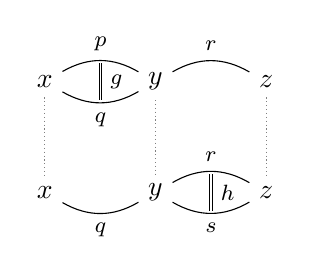
\begin{tikzpicture}[node distance=4em, baseline=(basenode.base)]
      \node[] (x1) {$x$};
      \node[right of=x1] (y1) {$y$};
      \node[right of=y1] (z1) {$z$};
      \node[below of=x1] (x2) {$x$};
      \node[right of=x2] (y2) {$y$};
      \node[right of=y2] (z2) {$z$};
      \draw[bend left] (x1) to node[above] (p) {\footnotesize$p$} (y1);
      \draw[bend right] (x1) to  node[below] (q1) {\footnotesize$q$} (y1);
      \draw[bend left] (y1) to node[above] (r1) {\footnotesize$r$} (z1);
      \draw[bend left] (y2) to node[above] (r2) {\footnotesize$r$} (z2);
      \draw[bend right] (y2) to  node[below] (s) {\footnotesize$s$} (z2);
      \draw[bend right] (x2) to node[below] (q2) {\footnotesize$q$} (y2);
      \draw[double, shorten >=.1em, shorten <=.1em] (p) to node[right] {\footnotesize$g$} (q1);
      \draw[double, shorten >=.1em, shorten <=.1em] (r2) to node[right] {\footnotesize$h$} (s);
      \draw[gray,densely dotted] (x1) to node (basenode){} (x2) (y1) to (y2) (z1) to (z2);
    \end{tikzpicture}%
    =%
    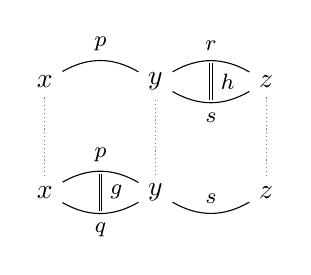
\begin{tikzpicture}[node distance=4em, baseline=(basenode.base)]
      \node[] (x1) {$x$};
      \node[right of=x1] (y1) {$y$};
      \node[right of=y1] (z1) {$z$};
      \node[below of=x1] (x2) {$x$};
      \node[right of=x2] (y2) {$y$};
      \node[right of=y2] (z2) {$z$};
      \draw[bend left] (x2) to node[above] (p) {\footnotesize$p$} (y2);
      \draw[bend right] (x2) to  node[below] (q1) {\footnotesize$q$} (y2);
      \draw[bend right] (y2) to node[above] (r1) {\footnotesize$s$} (z2);
      \draw[bend left] (y1) to node[above] (r2) {\footnotesize$r$} (z1);
      \draw[bend right] (y1) to  node[below] (s) {\footnotesize$s$} (z1);
      \draw[bend left] (x1) to node[above] (p2) {\footnotesize$p$} (y1);
      \draw[double, shorten >=.1em, shorten <=.1em] (p) to node[right] {\footnotesize$g$} (q1);
      \draw[double, shorten >=.1em, shorten <=.1em] (r2) to node[right] {\footnotesize$h$} (s);
      \draw[gray,densely dotted] (x1) to node (basenode){} (x2) (y1) to (y2) (z1) to (z2);
    \end{tikzpicture}%
    \caption{%
      Visual representation of~\cref{eq:horizontal-comp}. The vertical
      dotted lines denotes composition.%
    }\label{fig:horizontal-comp}
  \end{marginfigure}%
  This equality takes place in $r\cdot p = s\cdot q$ and is better
  represented by the diagram in~\cref{fig:horizontal-comp}. %
  One prove such a result by induction on $h$. Indeed, when
  $h\jdeq \refl r$, then both sides of the equation reduces through
  path algebra to $\ap {r\cdot\blank} (g)$. Now we are interested in
  this result when $x,y,z$ are all definitionally $a$, and $p,q,r,s$
  are all definitionally $\refl a$. In that case, one has that
  $\ap {\refl a\cdot \blank}$ and $\ap {\blank\cdot\refl a}$ both act
  trivially, and the equation becomes: $h\cdot g = g \cdot h$.

  One still has to prove that the function $\loopspace$ is an inverse
  for $\BB$. Given an abelian group $G$, the proof
  of~\cref{lemma:universal-cover-simply-connected} gives an
  equivalence between $\B\loopspace {(\BB G)}$ and the connected
  component of $\id_{\BG_\div}$ in $\BG_\div=\BG_\div$. By
  definition, this is the classifying type of $\grpcenter(G)$. Being
  abelian, $G$ is isomorphic to its center
  (\cref{def:abelian-groups}), and so it yields an element of
  $\loopspace {(\BB G)} =_{\typegroup} G$. %
  \marginnote[-1.5\baselineskip]{%
    If $X \ptdweq Y$ denote the type of pointed equivalences between
    pointed types $X,Y:\UUp$, then the univalence axiom implies that
    there is an equivalence
    \begin{displaymath}
      (X=Y) \weq (X \ptdweq Y).
    \end{displaymath}%
  }%
  Conversely, take a pointed simply connected $2$-type $(A,a)$. One
  wants to prove $\BB (\loopspace {(A,a)}) \weq_\ast (A,a)$. One
  should first notice that, because $\loopspace (A,a)$ is an abelian
  group,
  \begin{fullwidth}
  \begin{equation}
    \label{eq:loopspace-A-abelian}%
    {\B\loopspace \left( \BB (\loopspace {(A,a)}) \right)}
    \weq \conncomp{((a=a)=(a=a))}{\refl{a=a}} \weq (a=a,\refl a).
  \end{equation}
\end{fullwidth}
  This equivalence maps a path
  \begin{displaymath}
    (p,!):(a=a,\settrunc{\refl{a=a}})=(a=a,\settrunc{\refl{a=a}})
  \end{displaymath}
  to the evaluation $p(\refl a): a=a$.

  %% OLD MATERIAL, can still be useful.
  %%
  % We will now provide
  % \begin{displaymath}
  %   \Phi : \BB {(\loopspace {(A,a)})} \ptdto (A,a)
  % \end{displaymath}
  % such that $\loopspace(\Phi)$ is the previous equivalence.
  % To be able to
  % express $\Phi$, we need a small gadget about truncations of
  % function
  % types: for types $X,Y:\UU$, given an element
  % $f_0:\setTrunc{X\to Y}$, one constructs a map
  % $\lceil f_0 \rceil : \setTrunc X \to \setTrunc Y$; the type of
  % $\lceil f_0 \rceil$ being a set, one might as well suppose that
  % $f_0 \jdeq \settrunc f$ for some $f:X\to Y$; then we set
  % $\lceil f_0 \rceil (\settrunc x) = \settrunc{f(x)}$, which
  % suffices
  % in order to define $\lceil f_0 \rceil$ entirely because its
  % codomain
  % $\setTrunc Y$ is a set. If we assume the axiom of
  % choice\footnote{What is the status of AC in this book??}, then
  % $\lceil \blank \rceil$ is injective when $Y$ is a set.
  %%
  We will now define a pointed map
  $\Phi : (A,a) \ptdto \BB (\loopspace {(A,a)})$, and prove
  subsequently that this is an equivalence. Let $T : A \to \UU$ be the
  type family define by
  \begin{displaymath}
    T(a') \defequi \sum_{\alpha:\setTrunc{(a=a)\weq(a=a')}}
    \prod_{p:a=a'}\alpha=\settrunc {p\cdot\blank}
  \end{displaymath}
  We claim that $T(a')$ is contractible for all $a':A$. By
  connectedness of $A$, it is equivalent to showing that $T(a)$ is
  contractible. However
  \begin{align*}
    T(a)
    &\jdeq \sum_{\alpha:\setTrunc{(a=a)\weq(a=a)}}\prod_{p:a=a}
      \alpha = \settrunc {p\cdot \blank}
    \\
    &\weq \sum_{\alpha:\setTrunc{(a=a)\weq(a=a)}} \alpha = \settrunc{\id_{a=a}}
    \\
    &\weq 1
  \end{align*}
  Let then $\Phi (a')$ be the element
  $(a=a', \kappa_{a'}):\univcover \UU {a=a}$ where $\kappa_{a'}$ is
  the first projection of the center of contraction of $T(a')$. In
  particular, following the chain of equivalences above, $\Phi(a)$ is
  defined as $(a=a, \settrunc{\refl {a=a}})$, hence $\Phi(a)$ is
  trivially pointed by a reflexivity path. To verify that $\Phi$, thus
  defined, is an equivalence, one can use connectedness of
  $\BB(\loopspace (A,a))$ and only check that
  $\inv\Phi(a=a,\settrunc{\refl {a=a}})$ is contractible. However,
  \begin{displaymath}
    \inv\Phi(a=a,\settrunc{\refl {a=a}}) \simeq \sum_{a':A}
    \sum_{\varphi : (a=a) \weq (a=a')}\settrunc{\varphi} = \kappa_{a'}.
  \end{displaymath}
  For an element $a':A$ together with $\varphi: (a=a) \weq (a=a')$
  such that the proposition $\settrunc \varphi = \kappa_{a'}$ holds, a
  path between $(a,\id_{a=a},!)$ and $(a',\varphi,!)$ consists of a
  path $p:a=a'$ and a path $q:(x\mapsto p x) = \varphi$. We have a
  good candidate for $p$, namely $p\defequi \varphi(\refl
  a):a=a'$. However we don't have quite $q$ yet. Consider, for any
  $a':A$, the function
  \begin{fullwidth}
    \begin{displaymath}
      \ev_{\refl a}^{a'} :
      \left(
        (a=a, \settrunc{\refl{a=a}} ) =
        (a=a', \kappa_{a'} )
      \right)
      \to (a=a'),\quad (\psi,!) \mapsto \psi(\refl a) 
    \end{displaymath}
  \end{fullwidth}
  Note that $\ev_{\refl a}^{a}$ is precisely the equivalence
  $\loopspace{(\BB\loopspace(A,a))}\weq (a=a)$ described
  in~\cref{eq:loopspace-A-abelian}. Hence, by connectedness of $A$,
  one gets that the proposition $\isEq(\ev_{\refl a}^{a'})$ holds for
  all $a':A$. In particular, because the propositions
  $\settrunc \varphi = \kappa_{a'}$ and
  $\settrunc {p\cdot\blank} = \kappa_{a'}$ holds, one gets elements
  $(\varphi,!)$ and $(x\mapsto px,!)$ in the domain of
  $\ev_{\refl a}^{a'}$. Their image $\ev_{\refl a}^{a'}(\varphi,!)$
  and $\ev_{\refl a}^{a'}(x\mapsto px,!)$ are both equal to $p$, which
  provides a path $(x\mapsto px,!)=(\varphi,!)$ in the domain. The
  first component is the path $q:(x\mapsto px) = \varphi$ that we
  wanted.
\end{proof}


\section{$G$-sets vs $\abstr(G)$-sets}
\label{sec:Gsetsabstrconcr}
\marginnote{Recall from \cref{def:abstrGtorsors} that the type of $\abstr(G)$-set is
  $$Set_{\abstr(G)}^\abstr\defequi \sum_{\mathcal X:\Set}\Hom_\abstr({\abstr(G)},\abstr(\Sigma_{\mathcal X})).$$}

Given a group $G$ it should by now come as no surprise that the type of $G$-sets is equivalent to the type of $\abstr(G)$-sets.
According to \cref{lem:homomabstrconcr}
$$\abstr:\Hom(G,\Sigma_{\mathcal X})\to\Hom^\abstr(\abstr(G),\abstr(\Sigma_{\mathcal X}))$$
is an equivalence, where the group $\Sigma_{\mathcal X}$ (as a pointed connected groupoid) is the component of the groupoid $\Set$, pointed at $\mathcal X$.  The component information is moot since we're talking about pointed maps from $\BG$ and we see that $\Hom(G,\Sigma_{\mathcal X})$ is equivalent to $\sum_{F:\BG_\div\to\Set}(\mathcal X=F(\sh_G))$.  Finally, 
$$\mathrm{pr}:\sum_{\mathcal X}\sum_{F:\BG_\div\to\Set}(\mathcal X=F(\sh_G))\we 
(\BG_\div\to\Set),\quad \mathrm{pr}(\mathcal X,F,p)\defequi F
$$
is an equivalence (since $\sum_{\mathcal X}(\mathcal X=F(\sh_G))$ is contractible).  
Backtracking these equivalences we see that we have established
\begin{lemma}
  \label{lem:actionsconcreteandabstract}
  Let $G$ be a group.  Then the map
  $$\ev_{\sh_G}:\GSet\to\Set^\abstr_{\abstr(G)},\qquad \ev_{\sh_G}(X)\defequi(X(\sh_G),a_X)
$$
is an equivalence, where the action $a_X:\Hom^\abstr(\abstr(G), \abstr(\Sigma_{X(\sh_G)}))$ is given by transport $X:\USym G\defequi(\sh_G=\sh_G)\to (X(\sh_G)=X(\sh_G))$.
\end{lemma}
If $X$ is a $G$-set, $g:\USym G$ and $x:X(\sh_G)$, we seek forgiveness for writing $g\cdot x:X(\sh_G)$ instead of $\cast(a_X(g))(x)$.\footnote{and I ask forgiveness for strongly disliking the use of ``$\cast$'' as a name for some tacitly understood map!}

\begin{example}
  \label{ex:abstrandconj}
  Let $H$ and $G$ be groups.  Recall that the set of homomorphisms from $H$ to $G$ is a $G$-set in a natural way:
$$\Hom(H,G):\BG\to\Set,\quad \Hom(H,G)(y)\defequi \sum_{F:\BH_\div\to \BG_\div}(y=F(\sh_H)).$$

What abstract $\abstr(G)$-set does this correspond to?
In particular, under the equivalence $\abstr:\Hom(H,G)\to\Hom^\abstr(\abstr(H),\abstr(G))$, what is the corresponding action of $\abstr(G)$ on the abstract homomorphisms?

The answer is that $g:\USym G$ acts on $\Hom^\abstr(\abstr(H),\abstr(G))$ by postcomposing with conjugation $c^g$ by $g$ as defined in \cref{ex:conjhomo}.  

Let us spell this out in some detail:
If $(F,p):\Hom(H,G)(\sh_G)\defequi
 \sum_{F:\BH_\div\to \BG_\div}(\sh_G=F(\sh_H))$ and $g:\USym G$, then $g\cdot(F,p)\defequi(F,p\,g^{-1})$.  If we show that the action of $g$ sends $\abstr(F,p)$ to $c^g\circ\abstr(F,p)$ we are done.

Recall that $\abstr(F,p)$ consists of the composite 
$$\xymatrix{\USym H\ar[r]^-{F^=}&(F(\sh_H)=F(\sh_G))\ar[rr]^-{t\mapsto p^{-1}t\,p}&&\USym G},$$ 
(\ie $\abstr(F,p)$ applied to $q:\USym H $ is  $p^{-1}F^=(q)\,p$)  together with the proof that this is an abstract group homomorphism.  
We see that $\abstr(F,p\,g^{-1})$ is given by conjugation:
$q\mapsto(p\,g^{-1})^{-1}F^=(q)\,(p\,g^{-1})=g\,(p^{-1}F^=(q)\,p)\,g^{-1}$, or in other words $c^g\circ\abstr(F,p)$.
\end{example}
For reference we list the conclusion of this example as a lemma:
\begin{lemma}\label{lem:abstrandconj}
  If $H$ and $G$ are groups, then the equivalence of \cref{lem:actionsconcreteandabstract} sends the $G$-set $\Hom(H,G)$ to the $\abstr(G)$-set $\Hom^\abstr(\abstr(H),\abstr(G))$ with action given by postcomposing with conjugation by elements of $\abstr(G)$.
\end{lemma}

If $f:\Hom(G,G')$ is a homomorphism, then precomposition with $\Bf:\BG\to \BG'$ defines a map $$f^*:(G'\text{-}\Set)\to(G\text{-}\Set).$$
\marginnote{Recall that \cref{lem:eq-mono-cover} told us that $f$ is an epimorphism precisely when $\USym f$ is a surjection.}
We will have the occasion to use the following result which essentially says that if $f:\Hom(G,G')$ is an epimorphism, then $f^*$ embeds the type of $G'$-sets as some of the components of the type of $G$-sets.
\begin{lemma}
  \label{lem:epifullyfaithful}
  Let $G$ and $G'$ be groups and let $f:\Hom(G,G')$ be an epimorphism.
  Then the map $f^*:(G'\text{-}\Set)\to(G\text{-}\Set)$ (induced by precomposition with $\Bf:\BG\to \BG'$) is ``fully faithful'' in the sense that if $X,Y$ are $G'$-sets, then
$$f^*:(X=Y)\to(f^*X=f^*Y)
$$
is an equivalence.
\end{lemma}
\begin{proof}
  Evaluation at $\sh_G$  yields an injective map 
$$\mathrm{ev}_{\sh_G}:(f^*X=f^*Y)\to(X(f(\sh_G)=Y(f(\sh_G)))$$ and the composite 
$$\mathrm{ev}_{\sh_G}f^*=\mathrm{ev}_{f(\sh_G)}:(X=Y)\to(X(f(\sh_G)=Y(f(\sh_G)))$$
 is the likewise injective, so $f^*:(X=Y)\to(f^*X=f^*Y)$ is injective. 

For surjectivity, let $F':f^*X=f^*Y$ and write, for typographical convenience, $a:X(f(\sh_G)=Y(f(\sh_G))$ for $\mathrm{ev}_{\sh_G}F'\defequi F'_{\sh_G}$.  
By the equivalence between $G$-sets and $\abstr(G)$-sets, $F'$ is uniquely pinned down by $a$ and the requirement that for all $g'=f(g)$ with $g:\USym G$ the diagram 
$$\xymatrix{X(f(\sh_G))\ar@{=}[r]^{X({g'})}\ar@{=}[d]_{a}&
  X(f(\sh_G))\ar@{=}[d]_{a}\\
  Y(f(\sh_G))\ar@{=}[r]^{Y({g'})}&Y(f(\sh_G))}
$$
commutes.  Likewise, (using transport along the identity $p_f:\sh_{G'}=f(\sh_G)$) an $F:X=Y$ in the preimage of $a$ is pinned down by the commutativity of the same diagram, but with $g':f(\sh_G)=f(\sh_G)$ arbitrary (an a priori more severe requirement, again reflecting injectivity).   However, when $f:\USym G\to\USym {G'}$ is surjective these requirements coincide, showing that $f^*$ is an equivalence.


% Fix for the moment an  $a:X(f(\sh_G)=Y(f(\sh_G))$

% Now, by transport along the identity $p_f:\sh_{G'}=f(\sh_G)$ and the equivalence between $G'$-sets and $\abstr(G')$-sets, an identity $F':X=Y$ of $G'$-sets is uniquely pinned down by an identity $F'_{f(\sh_G)}:X(f(\sh_G)=Y(f(\sh_G))$ together with the proposition that for all $g':f(\sh_G)=f(\sh_G)$ the diagram $$\xymatrix{X(f(\sh_G))\ar@{=}[r]^{X_{g'}}\ar@{=}[d]_{F'_{f(\sh_G)}}&
%   X(f(\sh_G))\ar@{=}[d]_{F'_{f(\sh_G)}}\\
%   Y(f(\sh_G))\ar@{=}[r]^{Y_{g'}}&Y(f(\sh_G))}
% $$
% commutes.  Likewise, an identity $F:f^*X=f^*Y$ is given by exactly the same data, except that the diagram is only required to commute for $g'=f(g)$ for all $g:\USym G$.  But when $f:\USym G\to\USym {G'}$ these requirements coincide.


% ; $F:X=Y$ is in the preimage of $a:X(f(\sh_G)=Y(f(\sh_G))$ if and only if $a=F_{f(\sh_G)}$ and for all $g':f(\sh_G)=f(\sh_G)$ the diagram
% $$\xymatrix{X(f(\sh_G))\ar@{=}[r]^{X_{g'}}\ar@{=}[d]_{F_{f(\sh_G)}}&
%   X(f(\sh_G))\ar@{=}[d]_{F_{f(\sh_G)}}\\
%   Y(f(\sh_G))\ar@{=}[r]^{Y_{g'}}&Y(f(\sh_G))}
% $$
% commutes.  However, since $f$ is surjective there is a $g:\USym G$ so that $g'=f(g)$.  Therefore, anything in $f^*X=f^*Y$ which is in the preimage of $a$ is in the image of $f^*:X=Y$ and we have shown that $f^*$ is also a surjection.
\end{proof}



\section{Sums of groups}
\label{sec:coprod}
We have seen how the group of integers $\ZZ=(S^1,\base)$ synthesizes the notion of one symmetry with no relations: every symmetry of the circle is of the form $\Sloop^n$ for some unique $n$.  Also, given any group $G=\aut_A(a)$, the set $a=a$ of symmetries of $a$ corresponds to the set of homomorphisms $\ZZ\to G$, \ie to pointed functions $(S^1,\base)\to_*(A,a)$ by evaluation at $\Sloop$.  What happens if we want to study more than one symmetry at the time?  

For instance, is there a group $\ZZ\vee\ZZ$ so that for any group $G=\aut_A(a)$ a homomorphism $\ZZ\vee\ZZ\to G$ corresponds to {\bf two} symmetries of $a$?  
At the very least, $\ZZ\vee\ZZ$ itself would have to have two symmetries and these two can't have any relation, since in a general group $G=\aut_A(a)$ there is a priori no telling what the relation between the symmetries of $a$ might be.  
Now, \emph{one} symmetry is given by a pointed function $(S^1,\base)\to_*(A,a)$ and so a \emph{pair} of symmetries is given by a function $f:S^1+S^1\to A$ with the property that $f$ sends each of the base points of the circles to $a$.  But $S^1+S^1$ is not connected, and so not a group.  To fix this we take the clue from the requirement that both the base points were to be sent to a common base point and \emph{define} $S^1\vee S^1$ to be what we get from $S^1+S^1$ when we \emph{insert an identity} between the two basepoints.
\marginnote{$S^1\vee S^1$ if formed from $S^1+S^1$ by inserting an identity$$\xymatrix{\base\ar@(ul,dl)[]|{\Sloop}\ar@{.>}[rr]^{\text{identify!}}&&\base\ar@(ur,dr)[]|{\Sloop}}
  $$}

The amazing thing is that this works -- an enormous simplification of the classical construction of the ``free products'' or ``amalgamated sum'' of groups.  We need to show that the ``wedge'' $S^1\vee S^1$ is indeed a group, and this proof simultaneously unpacks the classical description.

We start by giving a definition of the wedge construction which is important for pointed types in general and then prove that the wedge of two groups is a group whose symmetries are arbitrary ``words'' in the original symmetries.

\begin{definition}
  \label{def:wedge}
  Let $(A_1,a_1)$ and $(A_2,a_2)$ be pointed types.  The \emph{wedge}\index{wedge of pointed types} is the pointed type $(A_1\vee A_2,a_{12})$ given as a higher inductive type by
  \begin{enumerate}
  \item functions $i_1:A_1\to A_1\vee A_2$ and $i_2:A_2\to A_1\vee A_2$
  \item an identity $g:i_1a_1=i_2a_2$.
  \end{enumerate}
We point this type at $a_{12}\defequi i_1a_1$.
  The function 
$$i^g_2:(a_2=_{A_2}a_2)\to(a_{12}=_{A_1\vee A_2}a_{12})$$ 
is defined by $i^g_2(p)\defequi g^{-1}i_2(p)g$, whereas (for notational consistency only) we set $i_1^g\defequi i_1:(a_1=_{A_1}a_1)\to(a_{12}=_{A_1\vee A_2}a_{12})$.
Simplifying by writing $i:A_1+A_2\to A_1\vee A_2$ for the function given by $i_1$ and $i_2$ (with basepoints systematically left out of the notation), 
the induction principle is
$$\prod_{C:(A_1\vee A_2)\to\UU}\sum_{s:\prod_{a:A_1+A_2}Ci(a)}
((s(a_1)=C(g^{-1})s(a_2))\,\to\,\prod_{x:(A_1\vee A_2)}C(x)).$$
\end{definition}

Unraveling the induction principle we see that if $B$ is a pointed type, then a  pointed function $f:A_1\vee A_2\to_* B$ is given by providing pointed functions $f_1:A_1\to_* B$ and $f_2:A_2\to_* B$  -- the identity $f_1(a_1)=f_2(a_2)$ which seems to be missing is provided by the requirement of the functions being pointed.  For the record
\begin{lemma}
  \label{lem:univvee}
  If $B$ is a pointed type, then the function 
  $$i^*:(A_1\vee A_2\to_*B)\to(A_1\to_*B)\times(A_2\to_*B),\qquad i^*(f)=(fi_1,fi_2)
$$
is an equivalence.
\end{lemma}



To the right you see a picture of $i_2^g(p)$: \marginnote{$$
\xy (-20,20)*+{};(-20,20)*+{}
**\crv{(15,20)&(18,20)&(-10,35)&(10,45)&(25,30)&(20,19)&(0,20)}
%?>*\dir{>}
?(0)*{} *!LD!/^-20pt/{i_1A_1}
?(.45)*{} *!LD!/^2pt/{>}
?(.95)*{} *!LD!/^-15pt/{g^{-1}}
?(.03)*{} *!LD!/^-5pt/{g}
?(.55)*{} *!LD!/^-7pt/{i_2p}
?(.65)*{} *!LD!/^-30pt/{i_2A_2}
?(.87)*{} *!LD!/^-12pt/{i_2a_2}
?(.86)*{} *!LD!/^-2pt/{\bullet}
?(1)*{} *!LD!/^-2pt/{\bullet}
?(1)*{} *!LD!/^-12pt/{a_{12}}
\endxy
$$}it is the symmetry of the base point $a_{12}\defequi i_1a_1$ you get by \emph{first} moving to $i_2a_2$ with $g$, \emph{then} travel around with $p$ ($i_2p$, really) and finally go home to the basepoint with the inverse of $g$.

\marginnote{The idea is that an identity in $a_{12}=x$ can be factored into a string of identities, each lying solely in $A_1$ or in $A_2$.  We define a family of sets consisting of exactly such strings of identities --  it is a set since $A_1$ and $A_2$ are groupoids -- and prove that it is equivalent to the family $P(x)\defequi(a_{12}=_{A_1\vee A_2}x)$ which consequently must be a family of sets.
We need to be able to determine whether a symmetry is reflexivity or not, but once we know that, the symmetries of the base point in the wedge are then given by ``words $p_0p_1\dots p_n$'' where the $p_j$ alternate between being symmetries in the first or the second group, and none of the $p_j$ for positive $j$ are allowed to be reflexivity.  Note that there order of the $p_j$s is not negotiable: if I shuffle them I get a new symmetry.}


\begin{definition}
  \label{def:sumofgroup}
  If $G_1=\aut_{A_1}(a_1)$ and $G_2=\aut_{A_2}(a_2)$ are groups, then their \emph{sum}\index{sum of groups} is defined as
  $$G_1\vee G_2\defequi \aut_{A_1\vee A_2}(a_{12}).$$
  The homomorphisms $i_1:G_1\to G_1\vee G_2$ and $i_2:G_2\to G_1\vee G_2$ induced from the structure maps  $i_1:A_1\to A_1\vee A_2$ and  $i_2:A_2\to A_1\vee A_2$ are also referred to as \emph{structure maps}.
\end{definition}
\begin{lemma}
  \label{lem:sumofgroupsISsum} If $G_1$, $G_2$ and $G$ are groups, then the function
  $$\Hom(G_1\vee G_2,G)\to\Hom(G_1,G)\times\Hom(G_2,G)$$ 
given by restriction along the structure maps is an equivalence.
\end{lemma}
\begin{proof}
  This is a special case of \cref{lem:univvee}.
\end{proof}
Specializing further, we return to our initial motivation and see that mapping out of a wedge of two circles \emph{exactly} captures the information of two independent symmetries:
\begin{corollary}
  \label{cor:ZplusZuniv}
  If $G$ is a group, then the functions
  $$\Hom(\ZZ\vee\ZZ,G)\to \Hom(\ZZ,G)\times\Hom(\ZZ,G)\simeq \USym G\times \USym G$$
  is an equivalence.
\end{corollary}
\begin{xca}
This leads to the following characterization of abelian groups formulated purely in terms of pointed connected groupoids (no reference to the identity types).
  \label{xca:whatAREabeliangroups}
  A group $G$ is abelian if and only if the canonical map
  
  \marginnote{$$\xymatrix{G\vee G\ar[r]^+\ar[d]_{\text{inclusion}}&G\\
      G\times G\ar@{.>}[ur]}$$}
$$+:G\vee G\to G$$ 
(given via \cref{lem:sumofgroupsISsum} by $\id_G:G\to G$) extends over the inclusion 
$$i:G\vee G\to G\times G$$ 
(given by the inclusions $\mathrm{in}_1,\mathrm{in}_2:G\to G\times G$).\footnote{I haven't written out a formalization myself}

As a cute aside, one can see that the required map $\BG\times\BG\to_*\BG$ actually doesn't need to be pointed:
factoring $+:\BG\vee\BG\to_*\BG$ over $i:\BG\vee\BG\to_*\BG\times\BG$
-- even in an unpointed way -- kills all ``commutators''
$ghg^{-1}h^{-1}:\USym(G\vee G)$.  
\end{xca}

We end the section by proving that wedges of decidable groups are decidable groups and that they can be given the classical description in terms of words.


\begin{lemma}
  \label{lem:wedgeofgpoidisgpoid}
  Let $G_1\defequi\aut_{A_1}(a_1)$ and $G_2\defequi\aut_{A_2}(a_2)$ be decidable groups, then the wedge sum $G_1\vee G_2\defequi\aut_{A_1\vee A_2}(a_{12})$ is a decidable group.  

Let $C_1$ be the set of strings $(p_0,n,p_1,\dots,p_n)$ with $n:\NN$ and, for $0\leq j\leq n$ 
\begin{itemize}
\item $p_{j}:\USym G_1%\defequi (a_1=a_1)
  $  for even $j$ 
\item $p_{j}:\USym G_2%\defequi (a_2=a_2)
  $ for odd $j$ and 
\item $p_j$ is not reflexivity for $j$ positive
\end{itemize}
(the last requirement makes sense and is a proposition since our groups are decidable).

  Then the function given by composition in $\USym G_{12}\defequi(a_{12}=a_{12})$
  $$\beta:C_1\to\USym G_{12}%\defequi(a_{12}=a_{12})
  ,\qquad\beta(p_0,n,p_1,\dots p_n)\defequi i_1^gp_0i_2^gp_1i_1^gp_2\dots i_?^gp_n$$ 
(where $i_?^gp_n$  is $i_1^gp_n$ or $i_2^gp_n$ according to whether $n$ is even or odd) is an equivalence.
\end{lemma}
\begin{proof}
  That the wedge is connected follows by transitivity of identifications,
  if necessary passing through the identification $g:i_1a_1=i_2a_2$ in the wedge.

We must prove that the wedge is a groupoid, \ie that all identity types are sets, which we do by giving an explicit description of the universal \covering. 

 We use the notation of \cref{def:wedge} freely, and for ease of notation, let $a_{2k+i}\defequi a_i$ and $i_{2k+i}^g\defequi i_i^g$ for $i=1,2$, $k:\NN$.  
Define families of sets
$$C_i:A_i\to\Set,\qquad i=1,2$$
by 
$$
C_i(x)\defequi(a_i=_{A_i}x)\times
\sum_{n:\NN}\prod_{1\leq k\leq n}\sum_{p_k:a_{i+k}= a_{i+k}}(p_k\neq\refl {a_{i+k}})
$$
when $x:A_i$.  Note that $p_k\neq\refl{a_{i+k}}$  is a proposition; we leave it out when naming elements. Hence, an element in $C_1(a)$ is a tuple
$(p_0,n,p_1,\dots,p_n)$ where $p_0:a_1=_{A_1}a$, $p_1:a_2=_{A_2}a_2$, $p_2:a_1=_{A_1}a_1$, and so on -- alternating between symmetries of $a_1$ and $a_2$, and where $p_0$ is the only identity allowed to be $\refl{}$. Define $C_{12}:C_1(a_1)\to C_2(a_2)$ by
$$C_{12}(p_0,n,p_1\dots,p_n)=
\begin{cases}
  (\refl{a_2}0,)&\text{ if }p_0=\refl{a_1}, n=0,\\
  (p_1,n-1,p_2\dots,p_n)& \text{ if }p_0=\refl{a_1},n\neq0,\\
  (\refl{a_2},n+1,p_0,\dots,p_n)& \text{ if }p_0\neq\refl{a_1}.
\end{cases}
$$
It is perhaps instructive to see a table of the values $C_{12}(p_0,n,p_1,\dots,p_n)$ for $n<3$:
\begin{center}
  \begin{tabular}{r|c cc}
    &$(p_0,0)$&$(p_0,1,p_1)$&$(p_0,2,p_1,p_2)$\\
    \hline
    $p_0=\refl{a_1}$&$(\refl{a_2},0)$&$(p_1,0)$&$(p_1,1,p_2)$\\
    $p_0\neq\refl{a_1}$&$(\refl{a_2},1,p_0)$&$(\refl{a_2},2,p_0,p_1)$&$(\refl{a_2},3,p_0,p_1,p_2)$
  \end{tabular}
\end{center}
Since $C_{12}$ is an equivalence, the triple $(C_1,C_2,C_{12})$ defines a family
$$C:A_1\vee A_2\to\Set.$$
In particular, $C(a_{12})\defequi C_1(a_1)$.
For $x:A_1$ we let $i^C_1:C_1(x)\to C(i_1(x))$ be the induced equivalence, and likewise for $i^C_2$.
We will show that $C$ is equivalent to $P\defequi \pathsp{a_{12}}$, where $P(x)\defequi(a_{12}=x)$, and so that the identity types in the wedge are equal to the sets provided by $C$.

One direction is by transport in $C$; more precisely, 
$$\alpha:\prod_{x:A_1\vee A_2}(P(x)\to C(x))$$ is given by transport with $\alpha(a_{12})(\refl{a_{12}})\defequi(\refl{a_{1}},0):C(a_{12})$. 
The other way, 
$$\beta:\prod_{x:A_1\vee A_2}(C(x)\to P(x))$$ is given by composing identities, using the glue $g$ to make their ends meet: 
$$\beta(i_1a)(p_0,n,p_1,\dots,p_n)\defequi i_1(p_0)i_2^g(p_1)i_3^g(p_2) \dots i_{n+1}^g(p_n)$$ 
(here the definition $\dots i_3^g\defequi i_1^g\defequi i_1$ proves handy since we don't need to distinguish the odd and even cases)   
and likewise 
$$\beta(i_2a)(p_0,n,p_1,\dots,p_n)\defequi i_2(p_0)g\,i_1^g(p_1)i_2^g(p_2) \dots i_{n}^g(p_n)$$ and compatibility with the glue $C_{12}$ is clear since the composite $\refl{x}p$ is equal to $p$.

For notational convenience, we hide the $x$ in $\alpha(x)(p)$ and $\beta(x)(p)$ from now on.

That $\beta\alpha(p)=p$ follows by path induction: it is enough to prove it for $x=a_{12}$ and
$p\defequi\refl{a_{12}}$:
$$\beta\alpha(\refl{a_{12}})=\beta(\refl{a_1},0)=i_1^g\refl{a_1}=\refl{a_{12}}.$$  

That $\alpha\beta(p_0,n,p_1\dots,p_n)=(p_0,n,p_1,\dots,p_n)$ follows by induction on $n$ and $p_0$.  For $n=0$ it is enough to consider  $x=a_{12}$ and $p_0=\refl{a_1}$, and then 
$\alpha\beta(\refl{a_1},0)\defequi\alpha(\refl{a_{12}})\defequi(\refl{a_1},0)$.  In general, (for $n>0$) 
\begin{align*}
  \alpha\beta(p_0,n,p_1\dots,p_n)
=&\trp[C]{i_1(p_0)i_2^g(p_1)i_1^g(p_2) \dots i_{n+1}^g(p_n)}(\refl{a_1,0})\\
=&\trp[C]{i_1(p_0)}\dots\trp[C]{i_{n+1}^g(p_n)}(\refl{a_1,0}).
\end{align*}
  The induction step is as follows: let $0< k\leq n$, then 
\begin{align*}
  &\trp[C]{i_k^gp_{k-1}}i^C_{k-1}(p_k,n-k-1,p_{k+1},\dots,p_n)\\
  =&\trp[C]{i_k^gp_{k-1}}i^C_k(\refl{a_{k-1}},n-k,p_k,\dots,p_n)\\
  =&i^C_k\trp[C_k]{p_{k-1}}(\refl{a_{k-1}},n-k,p_k,\dots,p_n)\\
  =&(p_{k-1},n-k,p_k,\dots,p_n).
\end{align*}
%((please see whether this makes sense to anybody but yvt))
\end{proof}

% Local Variables:
% fill-column: 144
% latex-block-names: ("lemma" "theorem" "remark" "definition" "corollary" "fact" "properties" "conjecture" "proof" "question" "proposition")
% TeX-master: "book"
% End:

\chapter{Subgroups}
\label{ch:subgroups}

\section{Subgroups}
\label{sec:subgroups}
In our discussion of the group $\ZZ=\aut_{S^1}(\base)$ of integers in we discovered that the ``subsymmetries'' formed a very organized structure.
For each natural number $n$ we obtained a set of subsymmetry the entire identity type $\base=\base$, namely the set of all the iterates $(\Sloop^{n})^m$ where $m$ varies over the integers.
When $n$ was positive this was realized as the $n$-fold \covering of $S^1$, when $n=0$ this was given by the universal \covering.


The other extreme of the idea of ``subsymmetries'' was exposed in \cref{sec:groupssubperm} in the form of the slogan ``any symmetry is a symmetry of $\Set$''.
By this we meant that, if $G=\aut_A(a)$ is a group, we produced a monomorphism $\rho_G:\Hom(\aut_a(A),\aut_{a=a}(\Set))$, \ie any symmetry of $a$ is uniquely given by a symmetry (``permutation'') of the set $a=a$.

For other groups the ``subsymmetries'' form more involved structures,
and there are several ways to pin them down.  If $A$ is a groupoid, singling out a group of subsymmetries of $a:A$ should be a way of picking out just some of the symmetries of $a$ in $A$ in a way so that we can compose subsymmetries compatibly.  To make a long story short; we want a group $H$ and a homomorphism $i:\Hom(H,G)$ so that $i^\abstr:\USym H\to\USym H$ is injective.\footnote{in classical set theory it is an important difference between saying that a function is the inclusion of a subset (which is what one classically wants) and saying that it is an injection.  We'll address this in a moment, so rest assured that all is well as you read on.}  We have a name for such a setup: $i$ is a \emph{monomorphism} as laid out in different intermpretations in \cref{lem:eq-mono-cover}.

\subsection{Subgroups as monomorphisms}

In particular, the proposition $\ismono(i)$ is equivalent to saying that $i^\abstr:\USym H\to \USym G$ is an injection (all preimages are propositions), and also to saying that $B i:\BH\to\BG$ is a \covering, and (since $\BG$ is connected), to $\isset((Bi)^{-1}(\sh_G))$.
%\newcommand{\typemono}{Mono}
\begin{definition}
  If $G$ is a group, the \emph{type of monomorphisms into $G$} is
  $$\typemono_G\defequi\sum_{H:\typegroup}\sum_{i:\Hom(H,G)}\ismono(i).$$
\end{definition}

\begin{example}
  Consider the  homomorphism $i:\Sigma_2\to\Sigma_3$ of permutation groups corresponding to $(?+\bn 1,\refl{\bn 3}):\fin_2\to_*\fin_3$ (sending $A$ to $A+\bn 1$).  This is a monomorphism since $i^\abstr:\USym\Sigma_2\to\USym\Sigma_3$ is an injection
  \marginnote{$$\xymatrix{&3\ar@{.}[dd]&\\&&\\
    1\ar@{-}[uur]\ar@{-}[rr]&&2\ar@{-}[uul]}$$}
  (if $\Sigma_3$ represent all symmetries of an equilateral triangle in the plane (with vertices $1$, $2$, $3$), then $i$ is represented by the inclusion of the symmetries leaving $3$ fixed; \ie reflection through the axis the passing through the vertex $3$ which is marked with dots in the picture to the right). 
\end{example}

We will be interested in knowing when two monomorphisms into $G$ are identical.

\begin{lemma}
  \label{lem:setofsubgroups}
  Let $G$ be a group and $(H,i_H,!),(H',i_{H'},!):\typemono_G$ be two monomorphisms into $G$.  The identity type $(H,i_H,!)=(H',i_{H'},!)$ is equivalent to
  \marginnote{$$\xymatrix{H\ar[rr]^f_\simeq\ar[dr]_{i_H}&&H'\ar[dl]^{i_{H'}}\\
    &G&}$$}
  $$\sum_{f:\Hom(H,H')}\isEq(f^\abstr)\times (i_{H'}=i_H f)$$ and is a proposition.
  In particular, the type $\typemono_G$ of monomorphisms into $G$ is a set.
\end{lemma}
\marginnote{If you're familiar with the set-theoretic flavor of things, you know that it is important to distinguish between subgroups and injective group homomorphisms.   
Our use of monomorphisms can be defended because two monomorphisms into $G$ are identified exactly if they differ by precomposition by an identity.  
In set-theoretic language this corresponds to saying that a subgroup is an injective abstract homomorphism \emph{modulo} the relation forcing that precomposing with an isomorphism yields identical subgroups.  
Classical set-theory offers the luxury of having a preferred representative in every equivalence class: namely the image of the injection, type theory does not.  We only know that the type $\typemono$ is a set.}
\begin{proof}
By \cref{lem:isEq-pair=} an identity between $(H,i_H,!)$ and $(H',i_{H'},!)$ is uniquely given by an identity $p:H'=_{\typegroup}H$ such that $i_{H'}=i_H\,p$ (a proposition since $\Hom(H',G)$ is a set).
  The description of the identity type follows since by univalence and \cref{lem:eqofconntypes}, the identity type $H=H'$ is equivalent to the set 
$$\sum_{f:\Hom(H,H')}\isEq(f^\abstr).$$  
% If $(H,i_H,!)$ is a subgroup of $G$, then

Now, $i_{H'}=i_Hf$ is equivalent to $i_{H'}^\abstr=i_H^\abstr f^\abstr$, and since $i_H^\abstr$ is an injection of sets there is at most one such function $f^\abstr$; translating back we see that there is at most one $f$, making $\sum_{f%:\Hom(H,H')
}\isEq(f^\abstr)\times (i_{H'}=i_H f)$ a proposition.  
% Consequently, the identity type
% $(H,i_H,!)=_{\typesubgroup_G}(H,i_H,!)$ is equivalent to the type of homomorphisms $f:\Hom(H,H)$ which are such that $!:i_H^==i_H^=f^=$ and such that $f^=$ is an equivalence (as we see in a moment this last requirement is redundant).  
% Now, since $(H,i_H,!)$ is a subgroup, $i_H^=$ is an injection of sets, which forces $!:f^==\refl{\USym H}$, which ultimately forces $f$ to be (identical to) the identity homomorphism. 
\end{proof}



\subsection{Subgroups through $G$-sets}

For many purposes it is useful to define ``subgroups'' slightly differently.
A monomorphism into $G$ consists of a group $H$ (pointed connected groupoid  $\BH$) and a pointed function $Bi:\BH\to_* \BG$ whose fibers are sets (a pointed \covering).  There is really no need to specify that $H$ is a groupoid: if $F:T\to \BG$ is a \covering, then $T$ is automatically a groupoid.  

On the other hand,  the type of \coverings over $\BG$ is equivalent to the type of $G$-sets: if $X:\BG\to\Set$ is a $G$-set, then the \covering is given by the first projection $\tilde X\to \BG$ where $\tilde X\defequi\sum_{y:\BG}X(y)$ and the inverse is obtained by considering the fibers of a \covering.  Furthermore, we saw in \cref{lem:conistrans} that $\tilde X$ being connected is equivalent to the condition $\istrans(X)$ of \cref{def:transitiveGset} claiming that the $G$-set $X$ is transitive. 

Hence, the type (set, really) $\typemono_G$ of monomorphisms into $G$ is equivalent to the type of pointed connected \coverings over $\BG$, which again is equivalent to the type $\typesubgroup_G$ of transitive $G$-sets $X:\BG\to\Set$ together with a point in $X(\sh_G)$.

\begin{definition}
  Let $G$ be a group then the set of \emph{subgroups of $G$} is
  $$\typesubgroup_G\defequi\sum_{X:\BG\to\Set}\sum_{\pt_{\sh_G}:X(\sh_G)}\mathrm{isTrans}(X).$$
  The preferred equivalence with the set of monomorphisms into $G$ is given by the function
  $$E:\typemono_G\to\typesubgroup_G\qquad (H,i,!)\mapsto E(H,i,!)\defequi ((Bi)^{-1},(\sh_H,p_i),!),$$
  where $i:\Hom(H,G)$ is as always given by $(Bi_\div,p_i):(\BH_\div,\sh_H)\to_*(\BG_\div,\sh_G))$; and where $(Bi)^{-1}:\BG\to\Set$ is the preimage $G$-set  and $(\sh_H,p_i):(Bi)^{-1}(y)\defequi \sum_{x:\BH}y=Bi(x)$ is the base point.
\end{definition}

Since the types of subgroups and monomorphisms into a group $G$ are equivalent (via $E$), we may informally refer to elements in either sets as ``subgroups''


The family of sets $\typesubgroup_G(y)$ where we let the element $y:\BG$ vary is by the same reasoning equivalent to the family $\typesubgroup_G'(y)$ which we for reference spell out in symbols.

\begin{definition}
  Let $G$ be a group and $y:\BG$, then the $G$-set of \emph{subgroups' of $G$} is
  $$\typesubgroup_G':\BG\to\Set,\qquad\typesubgroup_G'(y)\defequi\sum_{X:\BG\to\Set}\sum_{\pt_y:X(y)}\mathrm{isTrans}(X)$$
and the type of \emph{normal subgroups'} is the set of fixed points
$$\typenormal_G'\defequi\prod_{y:\BG}\typesubgroup_G'(y).$$
%A \emph{normal subgroup'} of $G$ is an element in $\typenormal_G'$.
\end{definition}
Likewise, in symbols, the above described equivalence between the families $\typesubgroup_G$ and $\typesubgroup_G'$ is provided by the map 
$$E(y):\typesubgroup_G(y)\to\typesubgroup_G'(y),\qquad E(H,F,p_F,!)=(F^{-1}, (\sh_H,p_F),!)
$$
(where $H$ is a group, $F:\BH_\div\to \BG_\div$ is a map and $p_F:y=F(\sh_H)$ an identity in $\BG$; and $F^{-1}:\BG\to\Set$ is $G$-set given by the preimages of $F$ and $(\sh_H,p_F):F^{-1}(y)\defequi \sum_{x:\BH}y=F(x)$ is the base point).  If $y$ is $\sh_G$ we follow our earlier convention of dropping it from the notation.


Since the families are equivalent we may use $\typesubgroup_G$ or $\typesubgroup_G'$ interchangeably.

------------------



.
One thing is that our concept of a subtype of $B$ is merely the first projection $\sum_{b:B}P(b)\to B$, where the $P$ is a family of propositions.
Another thing is that for group the ``sub'' refers to the associated abstract groups, so that ``$\BH$ is a subgroup of $\BG$'' should \emph{not} mean that ``$\BH$ is a subtype of $\BG$'', but that we have a group homomorphism $f:\Hom(H,G)$ so that the induced function $\USym H\to\USym G$ is an ``inclusion of a subset''.
In other words, we must have that $f$ is a ``monomorphism'' (see \cref{lem:injofsetsaremono}).




Now, as we saw in \cref{lem:injofsetsaremono}, that   $f:\Hom(H,G)$ is a monomorphism is equivalent to saying that $f:\USym H\to\USym G$ is an injection (preimages are propositions) which again is equivalent to the preimages of $\Bf:\BH\to \BG$ being sets.
We must choose one of these equivalent formulations for our concept of ``subgroup'', but will move freely between them as may be convenient in a particular case.
%Hence we get the following neat formulation.
    \begin{definition}
      \label{def:subgroup}
      Let $G$ be a group.  
      The \emph{type of subgroups of $G$}\index{type!subgroup} is the type
      $$\typesubgroup_G\defequi\sum_{H:\typegroup}\sum_{f:\Hom(H,G)}\isset(\Bf^{-1}(\sh_G)).$$
       A subgroup $(H,f,!)$ is
      \begin{enumerate}
      \item \emph{trivial}\index{trivial subgroup} if $\BH$ is contractible
      \item \emph{proper}\index{proper subgroup} if $\Bf$ is not an equivalence.
      \end{enumerate}
    \end{definition}
    \begin{remark}
      \label{rem:notationsubgroup}
      A note on notation is in order.  
If $(H,i,!)$ is a subgroup of a group $G$, tradition often permits us to relax the burden of notation; we may write ``a subgroup $i:H\subseteq G$'', or, if we don't need the name of $i:\Hom(H,G)$ in what follows, simply ``a subgroup $H\subseteq G$'' or ``a subgroup $H$ of $G$''.
    \end{remark}

\begin{lemma}
  \label{lem:setofsubgroups}
  If $G$ is a group, then the type $\typesubgroup_G$ of subgroups is a set.
\end{lemma}
\begin{proof}
An identity between two subgroups $i_H:H\subseteq G$ and $i_{H'}:H'\subseteq G$ is an identity $p:H'=_{\typegroup}H$ such that $i_{H'}=i_H\,p$ (a proposition since $\Hom(H',G)$ is a set).
  By univalence and \cref{lem:eqofconntypes}, the identity type $H=H'$ is equivalent to the set 
$$\sum_{f:\Hom(H,H')}\isEq(f^=:\USym H\to\USym {H'}).$$  
%If $(H,i_H,!)$ is a subgroup of $G$, then
Consequently, the identity type
$(H,i_H,!)=_{\typesubgroup_G}(H,i_H,!)$ is equivalent to the type of homomorphisms $f:\Hom(H,H)$ which are such that $!:i_H^==i_H^=f^=$ and such that $f^=$ is an equivalence (as we see in a moment this last requirement is redundant).  
Now, since $(H,i_H,!)$ is a subgroup, $i_H^=$ is an injection of sets, which forces $!:f^==\refl{\USym H}$, which ultimately forces $f$ to be (identical to) the identity homomorphism. 
\end{proof}
Not only is the type of subgroups  of $G$ a set, it is in a natural way (equivalent to the value at $\sh_G$ of) a $G$-set which we denote by the same name
$$%\typesubgroup_G:\BG\to\Set,\qquad 
\typesubgroup_G(y)\defequi \sum_{H:\typegroup}\sum_{f:\Hom(H,G)(y)}\isset(\Bf^{-1}(\sh_G)),$$
where  as in \cref{ex:HomHGasGset}  
$$\Hom(H,G)(y)\defequi\sum_{F:\BH_\div\to \BG_\div}(y=F(\sh_H))$$
is the $G$-set of homomorphisms from $H$ to $G$.
% In this interpretation, $(H,F,p,!):\typesubgroup_G(\sh_G)$ represents a subgroup of $G$ (so that $p:\sh_G=F(\sh_H)$).  An identity $g:\USym G$ acts on $\typesubgroup_G(\sh_G)$ by sending $(H,F,p,!)$ to $(H,F,p\,g^{-1},!)$.

\begin{definition}
  \label{def:conjactonsubgroups}
  If $G$ is a group, then the action of $G$ on the set of subgroups is called \emph{conjugation}. 


  \label{def:conjugate}
  If $(H,F,p,!):\typesubgroup_G(\sh_G)$ is a subgroup of $G$ and $g:\USym G$, then the subgroups  $(H,F,p,!),(H,F,p\,g^{-1},!):\typesubgroup_G(\sh_G)$ are said to be \emph{conjugate}\index{conjugate}. 
\end{definition}
\begin{remark}
  \label{rem:whyconjugate}
  The term ``conjugation'' may seem confusing as the %(abstract) 
action of $g:\USym G$ on a subgroup $(H,F,p,!):\typesubgroup_G(\sh_G)$ (where $p:x=F(\sh_H)$) is simply $(H,F,p\,g^{-1},!)$, which does not seem much like conjugation.  
However, as we saw in \cref{ex:abstrandconj}, under the equivalence $\abstr:\Hom(H,G)\we\Hom^\abstr(\abstr(H),\abstr(G))$, the corresponding action on $\Hom^\abstr(\abstr(H),\abstr(G))$ is exactly (postcomposition with) conjugation $c^g:\abstr(G)=\abstr(G)$.  
\footnote{The same phenomenon appeared in \cref{xca:HomZGvsAdG} where we gave an equivalence between the $G$-sets $\Hom(\ZZ,G)$ and $\Ad_G$ (where the action is very visibly by conjugation).}
% \end{remark}

% \begin{remark}
  \label{rem:conjactiononsubgroups}
 %  It is worthwhile to study this action a bit further.  Let $(H,f,!)$ be a subgroup of $G$ and let $g:\USym G$.  We can trade $f$ for $\abstr(f):\Hom^\abstr(\abstr(G),\abstr(H))$ whose underlying set map is the injection $\Bf^=:\USym H\to\USym G$. %We allow ourselves to write ``$f$'' instead of $\Bf^=$. 
% As we saw in \cref{ex:abstrandconj}, the action of $g$ postcomposes with conjugation $c^g:\USym G=\USym G$.
% Hence, if we represent a subgroup as 
% $$(H,\phi,!):\sum_{H:\typegroup}\sum_{\phi:\Hom^\abstr(\abstr(H),\abstr(G))}\isprop(\phi^{-1}(e_G)),$$ then
% $g\cdot(H,\phi,!)=(H,c^g\,\phi,!)$.

% Now, if $g$ comes from $H$, say, $\i_H(h)$
\end{remark}
Summing up the remark:
\begin{lemma}
  \label{lem:conjugationabstractly}
  Under the equivalence of \cref{lem:actionsconcreteandabstract} between $G$-sets and $\abstr(G)$-sets, the $G$-set $\typesubgroup_G$ corresponds to the $\abstr(G)$-set
$$\sum_{H:\typegroup}\sum_{\phi:\Hom^\abstr(\abstr(H),\abstr(G))}\isprop(\phi^{-1}(e_G))$$ of abstract subgroups of $\abstr(G)$, with action $g\cdot(H,\phi,!)\defequi(H,c^g\,\phi,!)$ for $g:\abstr(G)$, where  $c^g:\abstr(G)=\abstr(G)$ is conjugation as defined in \cref{ex:conjhomo}.
\end{lemma}


\begin{remark}
 %  If you're familiar with the set-theoretic flavor of things, you know that it is important to distinguish between subgroups and injective group homomorphisms.  
% Our use of ``subgroup'' can be defended as follows.  
% It corresponds in set-theoretic language to saying that a subgroup is an injective homomorphism \emph{modulo} the relation forcing that precomposing with an isomorphism yields identical subgroups.  
% Set-theory offers the luxury of having a representative in every equivalence class: namely the image of the injection, type theory does not.
\end{remark}

\sususe{The geometry of subgroups: some small examples}
\label{smallsubgpex}

As a teaser, and in order to get a geometric feel for the subgroups and their intricate interplay, it can be useful to have some fairly manageable examples to stare at.  
Some of the main tools for analyzing the geometry of subgroups are collected in \cref{sec:fingp} on finite groups, and we hope the reader will be intrigued by our mysterious claims and go on to study \cref{sec:fingp}.
That said, the examples we'll present are possible to muddle through by hand without any fancy machinery, but brute force is generally not an option and even for the present examples it is not something you want to show publicly.

When presenting the subgroups of a group $G$, three types are especially revealing: the set of subgroups $\typesubgroup_G(\sh_G)$, the \emph{groupoid of subgroups} $\typesubgroup(G)\defequi\sum_{y:\BG}\typesubgroup_G(y)$ and what we for now call the ``set of normal subgroups'' $\prod_{y:\BG}\typesubgroup_G(y)$.   Our local use of ``normal subgroup'' is equivalent to the official definition to come.  

The first projection $\typesubgroup(G)\to \BG$ is referred to as the \emph{\covering of subgroups}.

\footnote{Write out and fix the concrete examples (cyclic groups and $\Sigma_3$) commented out}
% \begin{remark}
% In  \cref{cha:circle} we studied the subgroups of the group of integers $G=\ZZ$ through \coverings over the circle $S^1$ (which we showed was equivalent to $B\ZZ$).
% We discovered a subgroup $n\ZZ$ for each natural number $n:\NN$ and in the groupoid $\typesubgroup({\ZZ})$ these sit as elements in separate components.  Each of these components are contractible (because addition is commutative: $\ZZ$ is an abelian group).

% In general, a component $K$ of the groupoid $\sum_{y:\BG}\typesubgroup_G(y)$ of subgroups of a group $G$ may be much more interesting. For one thing the, $K$ can contain many subgroups in the sense that the preimage of the first projection $K\to \BG$ is a set that may have many different elements; each representing a subgroup.  However, this set of subgroup will be a \emph{conjugacy class} of subgroups: the different subgroups are related by the conjugation action of $G$.  

% If $G$ is abelian this action is trivial, and $\sum_{y:\BG}\typesubgroup_G(y)$ consists of contractible components indexed over the subgroups of $G$.  Otherwise different subgroups may live in the same component of the groupoid of subgroups -- we'll see examples in a moment.

% In addition, the components will not in general be contractible, revealing the symmetries of the subgroups under the conjugation action.
% \end{remark}


% \begin{example}
%   The trivial group only has itself as a subgroup; the groupoid of subgroups and the set of normal subgroups are singletons.
% \end{example}
% \begin{example}
%   The cyclic group $C_p$ of prime order $p$ has only two subgroups, the trivial and the full subgroup itself and both are normal.  In fact, all subgroups of abelian groups are normal.  

% In general, the cyclic group $C_n$ of order $n$ has exactly one subgroup for each divisor $i$ of $n$.
% \end{example}


% \begin{example}
%   The group $C_2\times C_2$ has has no less than five subgroups: the trivial one, three subgroups that as groups (as opposed as \emph{sub}groups) are equivalent to $C_2$ and the full group $C_4$ itself.
% \end{example}
% \begin{remark}
%   The permutation group $\Sigma_3$ has four nontrivial proper subgroups.  Three conjugate subgroups isomorphic as groups to $C_2$ and one normal one which is as a group is isomorphic to $C_3$.  The component containing the copies of $C_2$ is equivalent to a circle.
% \end{remark}
\sususe{Kernels and cokernels}
\label{subsec:ker}

If $\phi:\Hom^\abstr(\mathcal G,\mathcal G')$ is an abstract group homomorphism, the preimage $\phi^{-1}(e_G)$ is a classically called the kernel of $\phi$ and the cokernel is the quotient set of $\mathcal G'$ by the relation that if $g:\mathcal G$ and $g':\mathcal G'$, then $g'\sim g'\cdot\phi(g)$.  
In our setup with a group homomorphism 
$$f:\Hom(G,G')\defequi(\BG\to_*\BG'),$$ the kernel and cokernel are just two aspects of the preimage 
$$(\Bf)^{-1}(\sh_{G'})\defequi\sum_{z:\BG}(\sh_{G'}=\Bf(z)):$$
 the cokernel is the set of components and the kernel is a preferred component.  This point of view makes it clear that the kernel is a subgroup whereas there is no particular reason for the cokernel to be more than a ($G'$-) set.
\begin{definition}
  \label{def:cokernel}
  Let $f:\Hom(G,G')\defequi(\BG\to_*\BG')$  be a homomorphism. %  The preimage $$f^{-1}(\sh_{G'})\defequi\sum_{z:\BG}(\sh_{G'}=f(z))$$
% is a groupoid containing important information about $f$.
The \emph{cokernel}\index{cokernel} of $f$ is the $G'$-set
\[
  \coker f:\BG'\to\Set,\qquad \coker f(z)\defequi  \Trunc{(\Bf)^{-1}(z)}_0.\text{\footnotemark}
\]
\footnotetext{set trunctation}
The associated $\abstr(G')$-set $\coker f(\sh_{G'})$ is also referred to as the cokernel of $f$.  If $f:\Hom(G,G')$ is clear from the context and displays $G$ as a subgroup of $G'$, we often write $G'/G$ for the cokernel of $f$.  

\end{definition}
\begin{definition}
  \label{def:kernel}
Let $f:\Hom(G,G')$  be a homomorphism.
Consider the element 
$$\sh_{\ker f}\defequi(\sh_G,p_f):(\Bf)^{-1}(\sh_{G'})$$ (where $p_f:\sh_{G'}=\Bf(\sh_G)$ is the part of $f$ claiming it is a pointed map). 
Define the \emph{kernel}\index{kernel}  of $f$ to be the group defined by the pointed component  of $\sh_{\ker f}$ in $(\Bf)^{-1}(\sh_{G'})$:
$$\ker f\defequi ((\Bf)^{-1}(\sh_{G'})_{(\sh_{\ker f})},\sh_{\ker f}).
$$ 
Written out,
$B\ker f_\div\defequi \sum_{z:\BG}\sum_{p:\sh_{G'}=f(z)}\Trunc{\sh_{\ker f}=(z,p)}.$  

The first projection $B\ker f\to_* \BG$ displays the kernel $\ker f$ as a subgroup of $G$ (\emph{sub}group since the preimages are equivalent to the sets $\sum_{p:\sh_{G'}=\Bf(z)}\Trunc{\sh_{\ker f}=(z,p)}$).  

A subgroup is said to be \emph{normal}\index{normal} if it is the kernel of a surjective homomorphism.\footnote{clarify the relation between the surjective homomorphism and the subgroup}
\end{definition}

\begin{definition}
\label{def:image}
The \emph{image}\index{image} of $f$ is the subgroup of $G'$ given by $B\image f\defequi \sum_{z:\BG'}\coker f(z)$ pointed at $\pt_{\image f}\defequi (\sh_{G'},|\sh_G,p_f|)$ together with the first projection $B\image f\to \BG'$ (plus the fact that $\coker f(z)$ is a set).\label{def:surjective}

The \emph{induced homomorphism} $\tilde f:\Hom(G,\image f)$ is given by sending $x:\BG$ to
$$B\tilde f(x)\defequi (\Bf(x),|x,\refl{\Bf(x)}|).$$ 

We say that the homomorphism $f$ is \emph{surjective}\index{surjective! group homomorphism} if $(\Bf)^{-1}(\sh_{G'})$ is connected.
%, or equivalently if $\image f\to G'$ is an equivalence.
\end{definition}
% \begin{remark}
%   \label{rem:cokerasGset}
%   If $f:\Hom(G,G')$ we notice that the abstract group $\abstr(G')$ acts on $\coker(f)\defequi\Trunc{f^{-1}(\sh_{G'})}_0$, making the cokernel an $\abstr(G')$-set.  If we prefer to talk about a $G'$-set, we consider the cokernel as the set-family $$\BG'\to\Set,\qquad z\mapsto   \Trunc{f^{-1}(z)}_0.$$  
% We will see this used most frequently when considerint inclusions of subgroups: if $H$ is a subgroup of $G$, then $G/H$ is a $G$-set.
% \end{remark}
In view of \cref{ex:charsurinj} below, the families  
$$\mathrm{issurj},\mathrm{isinj}:\Hom(G,G')\to\Prop
$$
of propositions that a given homomorphism is surjective or injective have several useful interpretations.
\begin{xca}
  \label{ex:charsurinj}
  Let $f:\Hom(G,G')$ Prove that
  \begin{enumerate}
  \item the following are equivalent
    \begin{enumerate}
    \item $f$ is a surjective homomorphism (\cref{def:surjective}),
    \item the cokernel of $f$ is contractible,
    \item the first projection $B\image f\to \BG$ is an equivalence
    \item the induced map of sets 
$f^=:\USym G\to\USym {G'}$ is a surjection
    \end{enumerate}
  \item the following are equivalent
    \begin{enumerate}
    \item $f$ is an injective homomorphism (\ie the induced map of sets 
$f^=:\USym G\to(\sh_{G'}\to\sh_{G'})$
is an injection)
\item the kernel of $f$ is trivial
\item $\Bf:\BG\to \BG'$ is a \covering.
\item the induced map $B\tilde f:\BG\to B\image f$ is an equivalence.
    \end{enumerate}
  \end{enumerate}
\end{xca}



Note that if $f:\Hom(G,G')$, then the composite of the induced homomorphism $\tilde f:\Hom(G,\image f)$ with the subgroup inclusion (first projection) of $\image f$ in $G'$ is $f$ by definition.  We will refer to this as the \emph{factorization of $f$ through its image}.

\begin{lemma}
  \label{lem:kerandcoker}
  \label{lem:countinggps}
  Let $f:\Hom(G,G')$ be a group homomorphism.  The induced homomorphism $\tilde f:\Hom(G,\image f)$ is a surjective homomorphims and $f$ factors as $\tilde f$ followed by the inclusion of the image of $f$ in $G'$.  The induced map $(B\tilde f)^{-1}(\pt_{\image f})\to (\Bf)^{-1}(\sh_{G'})$ induces an equivalence
  $$B\ker\tilde f\simeq B\ker f.$$
\end{lemma}
\begin{proof}
Only the last part needs further comment, but follows since since for $x:\BG$ the first projection from $\pt_{\image f}=(\Bf,|x,\refl{\Bf(x)}|)$ to $\sh_{G'}=f(x)$ is an equivalence (the fibers are true propositions).
  \footnote{\color{blue}  
 Also show counting results for the finite group part somewhere.} 
\end{proof}

Finally, the image factorization would have been useless were it not for the fact that it is unique:
\begin{lemma}
  \label{lem:uniquenessofimagefactorizationforgroups}
  Let $G,H,G'$ be groups, let $h:\Hom(G,H)$ and $j:\Hom(H,G')$ be homomorphisms and let $!:f=j\,h$.  If $h$ is surjective there is a unique homomorphism $t:\Hom(H,\image f)$ so that $\tilde f=t\, h$ and $j$ is $t$ composed with the first projection from $\image f$ to $ G'$.
\end{lemma}
\begin{proof}
  We've used that we're operating with groupoids to simplify the statement, but a similar statement follows generally by essentially the proof below if you keep track of the element in $f=j\,h$.  To simplify we drop the ``$B$''s from the notation, writing ``$f$'' instead of ``$\Bf$''.  

That $h$ is a surjective homomorphism amounts to saying that for $y:\BH$, then the set truncation $\Trunc{h^{-1}(y)}_0$ of the preimage is contractible, and so the first projection $\mathrm{pr_1}:\sum_{y:\BH}\Trunc{h^{-1}(y)}_0\to \BH$ is an equivalence.

For $y:\BH$, consider the map 
$$T_y:h^{-1}(y)\to f^{-1}(j y),\qquad T_y(x,p)\defequi (x,!_xj(p))$$ where $x:\BG$, $p:y=h(x)$ and $!_xj(p):j(y)=f(x)$ is the composite of $j(p):j(y)=j\,h(x)$ and $!:j\,h=f$ (as applied to $x$).  Performing set-truncation on $T_y$ and precomposing with the inverse of the first projection, we get a map
$$t:\BH%\sum_{y:\BH}\Trunc{h^{-1}(y)}_0
\to\sum_{z:\BG'}\Trunc{f^{-1}(z)}_0\oldequiv B\image f,\qquad Bt(y)\defequi(jy,|T_y|(q_y))$$
where $q_y:\Trunc{h^{-1}(y)}_0$ is the second projection of the inverse of the first projection.  The agreement of $t$ with $\tilde f$ and $j$ follows by construction.
\end{proof}

\begin{example}
  An example from linear algebra: let $A$ be any $n\times n$-matrix with nonzero determinant and with integer entries, considered as a homomorphism $A:\Hom(\ZZ^n,\ZZ^n)$.  Then the cokernel of $A$ is a finite set with cardinality the absolute value of the determinant of $A$.  You might want to picture this as a $|\det(A)|$-fold \covering of the $n$-fold torus $(S^1)^{\times n}$ by itself.
\end{example}


\sususe{Subgroups through $G$-sets}


Occasionally it is useful to define ``subgroups'' slightly differently.
As we've defined it a subgroup of a group $G$ of the form $(H,f,!)$ where $H$ is a group (pointed connected groupoid  $\BH$), $f:\BH\to_* \BG$ is a pointed map whose fibers are sets (a pointed \covering).  There is really no need to specify that $H$ is a group: if $F:T\to \BG$ is a \covering, then $T$ is automatically a groupoid.  

On the other hand,  the type of \coverings over $\BG$ is equivalent to the type of $G$-sets: if $X:\BG\to\Set$ is a $G$-set, then the \covering is given by the first projection $\tilde X\to \BG$ where $\tilde X\defequi\sum_{y:\BG}X(y)$ and the inverse is obtained by considering the fibers of a \covering.  Furthermore, we saw in \cref{lem:conistrans} that $\tilde X$ being connected is equivalent to the condition $\istrans(X)$ of \cref{def:transitiveGset} claiming that the $G$-set $X$ is transitive. 

Hence, the type (set, really) $\typesubgroup_G$ of subgroups of $G$ is equivalent to the type of pointed connected \coverings over $\BG$, which again is equivalent to the type $\typesubgroup_G'$ of transitive $G$-sets $X:\BG\to\Set$ together with a point in $X(\sh_G)$.  

The family of sets $\typesubgroup_G(y)$ where we let the element $y:\BG$ vary is by the same reasoning equivalent to the family $\typesubgroup_G'(y)$ which we for reference spell out in symbols.

\begin{definition}
  Let $G$ be a group and $y:\BG$, then the $G$-set of \emph{subgroups' of $G$} is
  $$\typesubgroup_G':\BG\to\Set,\qquad\typesubgroup_G'(y)\defequi\sum_{X:\BG\to\Set}\sum_{\pt_y:X(y)}\mathrm{isTrans}(X)$$
and the type of \emph{normal subgroups'} is the set of fixed points
$$\typenormal_G'\defequi\prod_{y:\BG}\typesubgroup_G'(y).$$
%A \emph{normal subgroup'} of $G$ is an element in $\typenormal_G'$.
\end{definition}
Likewise, in symbols, the above described equivalence between the families $\typesubgroup_G$ and $\typesubgroup_G'$ is provided by the map 
$$E(y):\typesubgroup_G(y)\to\typesubgroup_G'(y),\qquad E(H,F,p_F,!)=(F^{-1}, (\sh_H,p_F),!)
$$
(where $H$ is a group, $F:\BH_\div\to \BG_\div$ is a map and $p_F:y=F(\sh_H)$ an identity in $\BG$; and $F^{-1}:\BG\to\Set$ is $G$-set given by the preimages of $F$ and $(\sh_H,p_F):F^{-1}(y)\defequi \sum_{x:\BH}y=F(x)$ is the base point).  If $y$ is $\sh_G$ we follow our earlier convention of dropping it from the notation.


Since the families are equivalent we may use $\typesubgroup_G$ or $\typesubgroup_G'$ interchangeably.  
There is, however, a little explanation needed in order to see that the type $\typenormal_G$ of normal subgroups is equivalent to $\typenormal'_G$.
We do this by using the intermediate set of surjections from $G$:
\newcommand{\epi}{\mathrm{epi}}
\begin{definition}
  \label{def:typeepi}
  If $G$ is a group, then the \emph{set of surjections from $G$} is the set
$$\epi_G\defequi\sum_{G':\typegroup}\sum_{f:\Hom(G,G')}\mathrm{issurj}(f).$$
\end{definition}
Note that if $f:\Hom(G,G')$ is a surjective homomorphism and $e:G'=G''$ is an identity of groups, then $(G',f,!)$ and $(G'',f',!)$ are identitified via $e$, where $f':\Hom(G,G'')$ is the homomorphism given by the composite of $f$ and the homomorphism corresponding to $e$.

\begin{definition}
  \label{def:ker2}
  If $f:\Hom(G,G')$ is a homomorphism and $x,y:\BG$, set $P^f_y(x)\defequi (f(y)=f(x))$.
  Define $$\ker':\epi_G\to\typenormal_G'$$
  by $\ker'(G',f,!)(y)\defequi(P^f_y,\refl{f(y)},!)$.
\end{definition}

\begin{lemma}
  \label{lem:diagfornormal}
  The diagram
  $$\xymatrix{
  &\typenormal_G\ar[r]^{\subseteq}&\typesubgroup_G\ar[dd]_{\simeq}^{E}\\
  \epi_G\ar[ur]^{\ker}\ar[dr]_{ker'}&&\\
  &\typenormal_G'\ar[r]^{\subseteq}&\typesubgroup_G'}
$$
commutes, where the top composite is the image factorization of the kernel and the bottom inclusion is the inclusion of fixed points.
\end{lemma}
\begin{proof}
  Following $(G',f,!):\epi_G$ around the top to $\typesubgroup_G'$ yields the transitive $G$-set sending $y:\BG$ to the set $\sh_{G'}=f(y)$ together with the point $p_f:\sh_{G'}=f(\sh_G)$ while around the bottom we get the transitive $G$-set sending $y:\BG$ to the set $f(\sh_G)=f(y)$ together with the point $\refl{f(\sh_G)}:f(\sh_G)=f(\sh_G)$.  Hence, precomposition by $p_f$ gives the identity proving that the diagram commutes. 
\end{proof}
We will prove that both $\ker$ and $\ker'$ in the diagram of \cref{lem:diagfornormal} are equivalences, leading to the desired conclusion that the equivalence $E:\typesubgroup_G\we\typesubgroup_G'$ takes the subset $\typenormal_G$ identically to $\typenormal_G'$.  Actually, by the uniqueness of the image factorization shown in \cref{lem:uniquenessofimagefactorizationforgroups}, it is enough to show that $\ker'$ is an equivalence; we'll spell out the details.

We start with a small, but crucial observation.
\begin{lemma}
  \label{lem:evaliseqwhennormal}
  Let $N:\typenormal'_G$ be a normal subgroup' with $N(y)\oldequiv (X_y,\pt_y,!)$ for $y:\BG$.  Then for any $y,z:\BG$
  \begin{enumerate}
  \item the evaluation map
$$\mathrm{ev}_{yz}:(X_y=X_z)\to X_z(y),\qquad \mathrm{ev}_{yz}(f)=f_y(\pt_y)$$
is an equivalence and
  \item  the map $X:(y=z)\to(X_y=X_z)$ (given by induction via $X_{\refl y}\defequi\refl{X_y}$) is surjective.
  \end{enumerate}
\end{lemma}
\begin{proof}
To establish the first fact we need to do induction independently on $y:\BG$ and $z:\BG$ in $X_y(z)$ at the same time as we observe that it suffices (since $\BG$ is connected) to show that $\mathrm{ev}_{yy}$ is an equivalence.

% Induction on the index gives rise to the map $X:(y=z)\to(X_y=X_z)$ ($X_{\refl y}\defequi\refl{X_y}$) and t
The composite 
$$\mathrm{ev}_{yy}X:(y=y)\to X_yy$$ is determined by $\mathrm{ev}_{yy}X(\refl y)\oldequiv \pt_y$. 
By transitivity of $X_y$ this composite is surjective, hence $\mathrm{ev}_{yy}$ is surjective too.  

On the other hand, in  \cref{lem:evisinjwhentransitive} we used the transitivity of $X_y$ to deduce that $\mathrm{ev}_{yy}$ was injective.  Consequently $\mathrm{ev}_{yy}$ is an equivalence.  But since $\mathrm{ev}_{yy}$ is an equivalence and $\mathrm{ev}_{yy}X$ is surjective we conclude that $X$ is surjective
\end{proof}
\begin{definition}
\label{def:normalquotient}
  Let $N:\typenormal'_G$ be a normal subgroup' with $N(y)\oldequiv (X_y,\pt_y,!)$ for $y:\BG$.  The \emph{quotient group}\index{quotient group} $G/N$ is the group defined as the component of the groupoid of $G$-sets containing and pointed at $X_{\sh_G}$.  

The \emph{quotient homomorphism}\index{quotient homomorphism} is the homomorphism $q_N:\Hom(G,G/N)$  defined by $Bq_N(z)=X_z$ (strictly pointed).  By \cref{lem:evaliseqwhennormal} $q_N$ is surjective and we have defined a map
$$q:\typenormal_G'\to\epi_G,\qquad q(N)=(G/N,q_N,!).$$
\end{definition}

\begin{remark}
It is instructive to see how the quotient homomorphism $Bq_N:\BG\to \BG/N$ is defined in the torsor interpretation of $\BG$.  If $Y\colon \BG\to\UU$ is a $G$-type we can define the quotient as
$$
Y/N:\BG\to\UU,\qquad Y/N(y)\defequi\sum_{z:\BG}Y(z)\times X_z(y).
$$
We note that in the case $\princ G(y)\defequi (\sh_G=y)$ we get
that 
$
\princ G /N(y)\defequi\sum_{z:\BG}(\sh_G=z)\times X_z(y)
$
is equivalent to $X_{\sh_G}$.  Consequently, if $Y$ is a $G$-torsor, then $Y/N$ is in the component of $X_{\sh_G}$ and we have
$$-/N:\typetorsor_G\defequi (G\text{-set})_{(\princ G)}\to (G\text{-set})_{(X_{\sh_G})}.
$$ Our quotient homomorphism $q_N:\Hom(G,G/N)$ is the composite of the equivalence $\pathsp{}^G:\BG\we\typetorsor_G$ of \cref{lem:BGbytorsor} and the quotient map $-/N$.
\end{remark}
\begin{lemma}
  \label{lem:qeq}
  The map $\ker':\epi_G\to\typenormal_G'$ is an equivalence with inverse $q:\typenormal_G'\to\epi_G$.
\end{lemma}
\begin{proof}
  Assume $N:\typenormal_G'$ with $N(y)\defequi(X_y,\pt_y,!)$ for $y:\BG$.  Then $\ker' q(N):\BG\to\Set$ takes $y:\BG$ to $(\ker' q(N))(y)\oldequiv(Y_y,\refl{X_y},!)$, where $Y_y(z)\defequi (X_y=X_z)$.  Noting that the equivalence $\mathrm{ev}_{yz}:(X_y=X_z)\we X_z(y)$ of \cref{lem:evaliseqwhennormal} has $\mathrm{ev}_{yy}(\refl{X_y})\defequi \pt_y$ we see that univalence gives us the desired identity $\ker' q(N)=N$.\footnote{fix so that it adhers to dogmatic language and naturality in $N$ is clear}

Conversely, consider a surjective homomorphism $f:\Hom(G,G')$.  
For $x:\BG$ and $z:\BG'$ let $Q^f_z(x)\defequi (z=f(x))$.  
Then the quotient group $G/\ker'(f)$ is the component  of the groupoid of $G$-sets containing and pointed at $Q^f_{f(pt_G)}$ and the quotient homomorphism $q_{\ker' f}:\BG\to_* \BG/\ker' f$ is given by  $q_{\ker' f}(y)\defequi Q^f_{f(y)}$ (strictly pointed -- \ie by $\refl{Q^f_{f(\sh_G)}}$). 
Observe that by using the identification of the basepoint $Q^f_{f(\sh_G)}$ of $\BG/\ker'f$ with $Q^f_{\sh_{G'}}$ given by $p_f:\sh_{G'}=f(\sh_G)$ we have defined a homomorphism $Q^f:\Hom(G',G/\ker'f$) such that 
 $$\xymatrix{&\BG\ar[dl]_f\ar[dr]^{q_{\ker'f}}&\\
 \BG'\ar[rr]_{Q^f}&&\BG/\ker'f
}$$
commutes.
We are done if we can show that $Q^f$ is an equivalence.
The preimage of the base point $Q^f_{f(\sh_G)}$ is
$$\sum_{z:\BG'}\prod_{y:\BG}(z=f(y))=(f(\sh_G)=f(y))$$ 
which by 
\cref{lem:epifullyfaithful} is equivalent to
$$\sum_{z:\BG'}\prod_{v:\BG'}(z=v)=(f(\sh_G)=v)$$
which by \cref{lem:pathsptransportiseq} is equivalent to the contractible type $\sum_{z:\BG'}z=f(\sh_G)$.
\end{proof}

\begin{corollary}
  \label{cor:normalisnormal}
  The kernel $\ker:\epi_G\to \typenormal_G$ is an equivalence of sets.
\end{corollary}
\begin{proof}
  Since $\ker':\epi_G\to\typenormal_G'$ and $E:\typesubgroup_G\to\typesubgroup_G'$ are equivalences and the diagram in \cref{lem:diagfornormal} commutes, the kernel from $\epi_G$ to $\typesubgroup_G$ is an injection.  Hence, given a normal subgroup, the type of epimorphisms of which it is the kernel is contractible.
\end{proof}

With this much effort in proving that our two perspectives on the concept of normal subgroups are the same, it can be worthwhile to make the composite equivalence
$$\ker\,q:\typenormal_G'\we\typenormal_G$$
explicit.   Let $N:\typenormal'_G$ be a normal subgroup' with $N(y)\oldequiv (X_y,\pt_y,!)$ for $y:\BG$ with $X_y:\BG\to\Set$, $\pt_y:X_y(y)$ and $!:\mathrm{isTrans}(X_y)$. 
Then 
$$(B\ker q_N)_\div\defequi\sum_{z:\BG}(X_z=X_{\sh_G})$$
pointed at $(\sh_G,\refl{X_{\sh_G}})$ and with $i_{\ker f}:B\ker q_N\to_*\BG$ given by the first projection.  This can be simplified somewhat:

\begin{definition}
  \label{def:associatednormal}
  Let $N:\typenormal'_G$ be a normal subgroup' with $N(y)\oldequiv (X_y,\pt_y,!)$ for $y:\BG$ with $X_y:\BG\to\Set$, $\pt_y:X_y(y)$ and $!:\mathrm{isTrans}(X_y)$.  Define a subgroup $(\mathrm{ass}(N),i_N,!)$ of $G$, called the \emph{associated normal subgroup}, as follows:
  \begin{enumerate}
  \item the connected groupoid $B\mathrm{ass}(N)_\div\defequi\sum_{z:\BG}X_{\sh_G}(z)$,
  \item together with the point $\pt_N\defequi(\sh_G,\pt_{\sh_G})$,
  \item the first projection $\Bi:B\mathrm{ass}(N)\to_*\BG$
  \item together with the assertion that the preimages of $\Bi$ (which are equivalent to $X_{\sh_G}(z)$ for varying $z:\BG$) are sets. 
  \end{enumerate}
\end{definition}


We obviously need to show that the ``normal'' in the name is warranted.
\begin{lemma}
  \label{lem:normalsarekernels}
The map
$$\mathrm{ev}:B\ker q_N\to B\mathrm{ass}(N),\qquad \mathrm{ev}(z,f)\defequi(z,f(\pt_z))$$ is an equivalence and furthermore commutes with the first projections to $\BG$.  The pointed map $\mathrm{ev}_*\defequi(\mathrm{ev},\refl{(\sh_G,\pt_{\sh_G})}):B\ker q_N\to_* B\mathrm{ass}(N)$
(well defined since $\mathrm{ev}(\sh_G,\refl{X_{\sh_G}})\defequi (\sh_G,\pt_{\sh_G})$) induces an identification of the subgroups $\ker\,q(N)$ and $\mathrm{ass}(N)$.  

Provided with this information, the associated normal subgroup $\mathrm{ass}(N)$ \emph{is} a normal subgroup and we get a commuting diagram
$$\xymatrix{&\typenormal_G\\
\epi_G\ar[ur]^{\ker}_{\simeq}\ar[dr]^{\ker'}_\simeq&\\
&\,\typenormal_G'.\ar[uu]^{\mathrm{ass}}_\simeq}$$
  
  % The associated normal subgroup of $N:\typenormal_G'$ is a normal subgroup; more precisely $N(\sh_G)$ is the kernel of the quotient homomorphism $q_N:\Hom(G,G/N)$.
  % Let $N:\typenormal'_G$ be a normal subgroup' with $N(y)\defequi (X_y,\pt_y,!)$ for $y:\BG$ with $X_y:\BG\to\Set$, $\pt_y:X_y(y)$ and $!:\mathrm{isTrans}(X_y)$.  Define a subgroup $(\mathrm{ass}(N),i_N,!)$ of $G$ as follows:
  % \begin{enumerate}
  % \item the connected groupoid $B\mathrm{ass}(N)_\div\defequi\sum_{z:\BG}X_{\sh_G}(z)$,
  % \item together with the point $\pt_N\defequi(\sh_G,\pt_{\sh_G})$,
  % \item the first projection $\Bi:B\mathrm{ass}(N)\to_*\BG$
  % \item together with the assertion that the preimages of $\Bi$ (which are equivalent to $X_{\sh_G}(z)$ for varying $z:\BG$) are sets. 
  % \end{enumerate}
  % Then $(\mathrm{ass}(N),i_N,!)$ is a normal subgroup of $G$ in the sense that it is the kernel of a homomorphism.
\end{lemma}
\begin{proof}
  % Let $N(y)\oldequiv (X_y,\pt_y,!)$ for $y:\BG$.  Let $G/N$ be the group defined as the component of the groupoid of $G$-sets containing and pointed in $X_{\sh_G}$.  Let $f:\Hom(G,G/N)$ be the homomorphism defined by $\Bf(z)=X_z$.
 %  Consider the kernel of the quotient homomorphism $q_N:\Hom(G,G/N)$ of \cref{def:normalquotient},
% $$(B\ker q_N)_\div\defequi\sum_{z:\BG}(X_z=X_{\sh_G})$$
% pointed in $(\sh_G,\refl{X_{\sh_G}})$ and with $i_{\ker f}:B\ker q_N\to_*\BG$ given by the first projection.  Consider t

% We claim that $\mathrm{ev}$ is an equivalence.
Compared with the proof of $\ker'$ being an equivalence (\cref{lem:qeq}) there are no new ingredients.
Since $B\mathrm{ass}(N)$ is connected it is enough to show that the preimage of $\mathrm{ev}^{-1}(\sh_G,\pt_{\sh_G})$ is contractible.  
Since $\mathrm{ev}$ agrees with the projections to $\BG$, the preimage is equivalent to $\sum_{f:X_{\sh_G}=X_{\sh_G}}f(\pt_{\sh_G})=\pt_{\sh_G}$.  We recognize this as the preimage $\mathrm{ev}_{{\sh_G}{\sh_G}}^{-1}(\pt_{\sh_G})$
of the evaluation map 
$\mathrm{ev}_{{\sh_G}{\sh_G}}:(X_{\sh_G}=X_{\sh_G})\to X_{\sh_G}(\sh_G)$ which is an equivalence by \cref{lem:evaliseqwhennormal}.  
% the preimage $\mathrm{ev}_{X_{\sh_G}}^{-1}(\pt_{\sh_G})$
% of the evaluation map 
% $\mathrm{ev}_{X_{\sh_G}}:(X_{\sh_G}=X_{\sh_G})\to X_{\sh_G}(\sh_G)$.  
% In \cref{lem:evisinjwhentransitive} %{lem:conistrans} 
% we proved that (since $X_{\sh_G}$ is transitive) $\mathrm{ev}_{X_{\sh_G}}$ is an injection.  Hence the preimage is a proposition, but since it contains $(\refl{X_{\sh_G}},\refl{\pt_{\sh_G}})$ it is contractible. 

Evoking univalence we get an identification of subgroups between the kernel of $f$ and $(\mathrm{ass}(N),i_N,!)$.
\end{proof}


\begin{remark}
  Where did we use that $N$ was a fixed point of the $G$-set $\typesubgroup_G'$?  If $Y:\BG\to\Set$ is a transitive $G$-set and $\sh_H:Y(\sh_G)$, then surely we could consider the group $W$ defined as the component of the groupoid of $G$-sets containing and pointed at $Y$.  The first problem is that we wouldn't know how to construct a homomorphism from $G$ to $W$ which we then could consider the kernel of.  The second problem is that we'd be stuck at the very end where we 
used \cref{lem:evaliseqwhennormal} to show that the evaluation map is an equivalencs; if we only had transitivity we could use \cref{lem:evisinjwhentransitive} to pin down injectivity, but surjectivity needed the extra induction freedom. 
\end{remark}

Summing up, using the various interpretations of subgroups, we get the following list of equivalent sets all interpreting what a normal subgroup is.  
%The explicit equivalences are left out of the statements.
\begin{lemma}
  \label{lem:characterizations of normal}
  Let $G$ be a group, then the following sets are equivalent
\begin{enumerate}
\item The set $\epi_G$ of surjective homomorphisms from $G$,
\item the set $\typenormal_G$ of kernels of surjections from $G$,
\item the set $\typenormal_G'$ of fixed points of the $G$-set $\typesubgroup_G'$,
\item the set of fixed points of the $G$-set $\typesubgroup_G$
\item the set of fixed points of the $G$-set of abstract subgroups of $\abstr(G)$ of \cref{lem:conjugationabstractly}.
\end{enumerate}
\end{lemma}


% The associated normal subgroup defines an equivalence from $\typenormal_G'$ to the type $\typenormal_G$ of kernels of surjective homomorphism. To see this we construct an inverse.

% \begin{definition}
%   \label{def:kerneltofixedpoint}
%   Let $f:\Hom(G,G')$ be a surjective homomorphism.  For $y,z:\BG$ consider the set $X_y^f(z)\defequi (f(z)=f(y))$ and the element $\pt^f_y\defequi\refl{f(y)}:X_y(y)$.  The $G$-set $X_y:\BG\to\Set$ is transitive since $f$ is surjective and so we have a map 
% $$\mathrm{ssa}:\typenormal_G\to\typenormal_G',\qquad \mathrm{ssa}(f)(y)\defequi(X_y^f,\pt_y^f,!).$$
% \end{definition}

% \begin{lemma}
%   \label{lem:characterizations of normal}
%   Let $G$ be a group, then the associated normal subgroup is an equivalence
%   $$\mathrm{ass}:\typenormal_G'\to\typenormal_G$$
% with inverse $\mathrm{ssa}$.  Summing up the following sets are equivalent
% \begin{enumerate}
% \item The set $\typenormal_G$ of kernels of surjections from $G$,
% \item the set $\typenormal_G'$ of fixed points of the $G$-set $\typesubgroup_G'$,
% \item the set of fixed points of the $G$-set $\typesubgroup_G$
% \item the set of fixed points of the $G$-set of abstract subgroups of $\abstr(G)$.
% \end{enumerate}
% \end{lemma}
% \begin{proof}
%   The last three entries are equivalent since they are the fixed points of equivalent $G$-sets, so we only need to comment on the first assertion.

% Let $f:\Hom(G,G')$ be a surjective homomorphism.  
% The kernel $N\oldequiv \ker f$ is then given by the first projection 
% $$\text{pr}:\sum_{z:\BG}\sh_{G'}=\Bf(z)\to_*\BG.$$
% Then $\mathrm{ass\,ssa}(\ker f)$ defined to be
% $$
% (\sum_{z:\BG}\prod_{y:\BG}
% (\pathsp{f(\sh_G)}^{G'}{f(y)}=\pathsp{f(z)}^{G'}{f(y)},
% \text{pr}, (\sh_G,\refl{\pathsp{f(\sh_G)}^{G'}{f(\sh_G)}},!),$$
% where $\pathsp{a}^{G'}{b}\defequi (a=b)$ for $a,b:\BG'$.
% The desired identification between $\ker f$ and $\mathrm{ass\,ssa}(\ker f)$ is then given by composing the identifications
% $\preinv(p_f):(\sh_{G'}=f(z))=(f(\sh_G)=f(z))$ and 
% $$\preinv:(f(\sh_G)=f(z))=
% \prod_{y:\BG}(\pathsp{f(\sh_G)}^{G'}{f(y)}=\pathsp{f(z)}^{G'}{f(y)})$$
% \footnote{((find ref where this was demonstrated: slight modification since we only claim naturality in $G$)).}
% \end{proof}



% There are many valuable constructions to be extracted from the proof of \cref{lem:normalsarekernels}.
% \begin{definition}
%   \label{def:associatedquotient}
% \end{definition}
% \footnote{COMEBACK 190509 Do the converse and elevate constructions to definitions}



\sususe{The pullback}
\label{sec:pullback}

\begin{definition}
  \label{def:pullback}
  Let $B, C, D$ be types and let $f:B\to D$ and $g:C\to D$ be two maps.  
The \emph{pullback}\index{pullback} of $f$ and $g$ is the type 
$$\prod(f,g)\defequi\sum_{(b,c):B\times C}(f(b)=_Dg(c))$$
together with the two projections $\prod(f,g)\to B$ and $\prod(f,g)\to C$ sending $(b,c,p):\prod(f,g)$ to $b:B$ or $c:C$.  If $f$ and $g$ are clear from the context, we may write $B\times_DC$ instead of $\prod(f,g)$ and summarize the situation by the diagram
$$\xymatrix{B\times_DC\ar[r]\ar[d]&C\ar[d]^g\\B\ar[r]^f&\,D.}$$
\end{definition}
\begin{xca}
  \label{xca:univpropofpullback}
  Let $f:B\to D$ and $g:C\to D$ be two maps with common target.  If $A$ is a type show that 
  \begin{align*}
    (A\to B)\times_{(A\to D)}(A\to C)\to &(A\to B\times_DC)\\ 
(\beta,\gamma,p:f\beta=g\gamma)\,\mapsto\,&(a\mapsto (f(a),g(a),p(a):f\beta(a)=g\gamma(a)))
  \end{align*}
 is an equivalence.
\end{xca}

\begin{example}
  If $g:\bn 1\to D$ has value $d:D$ and $f:B\to D$ is any map, then $\prod(f,g)\oldequiv B\times_D\bn 1$ is equivalent to the preimage $f^{-1}(d)\defequi\sum_{b:B}d=f(b)$.
\end{example}
\begin{example}
  \label{ex:pullbackandgcd}
  Much group theory is hidden in the pullback.  For instance, the greatest common divisor $\gcd(a,b)$ of $a,b:\NN$ is another name for the number of components you get if you pull back the $a$-fold and the $b$-fold cover of the circle: as we will see in \cref{lem:iso2} we have a pullback
$$\xymatrix{S^1\times C_{\gcd(a,b)}\ar[d]\ar[r]& S^1\ar[d]^{(-)^b}\\
S^1\ar[r]^{(-)^a}&\,S^1}
$$ 
(where $C_n$ was the cyclic group of order $n$).
To get a geometric idea, think of the circle as the unit circle in the complex numbers so that the $a$-fold cover is simply taking the $a$-fold power.  With this setup, the pullback should consist of pairs $(z_1,z_2)$ of unit length complex numbers with the property that $z_1^a=z_2^b$.  Let $a=a'G$ and $b=b'G$ where $G=\gcd(a,b)$. Taking an arbitrary unit length complex number $z$, then the pair $(z^{b'},z^{a'})$ is in the pull back (since $a'b=ab'$).  But so is $(\zeta z^{b'},z^{a'})$, where $\zeta$ is any $G$-th root of unity.  Each of the $G$-choices of $\zeta$ contributes in this way to a component of the pullback.  In more detail: identifying the cyclic group $C_G$ of order $G$ with the group of $g$-th roots of unity, the top horizontal map $S^1\times C_G\to S^1$ sends $(z,\zeta)$ to $z^{a'}$ and the left vertical map sends $(z,\zeta)$ to the product $\zeta z^{b'}$.  

Also the least common multiple is hidden in the pullback; in the present example it is demonstrated that the map(s) accross the diagram makes each component of the pullback a copy of the subgroup $a'b\ZZ$ of $\ZZ$.
\end{example}


\begin{definition}
  \label{def:intersectionand unionofsets}
  Let $S$ be a set and consider two subsets $A$ and $B$ of $S$ given by two families of propositions (for $s:S$) $P(s)$ and $Q(s)$.  The \emph{intersection}\index{intersection! of sets} $A\cap B$ of the two subsets is given by the family of propositions $P(s)\times Q(s)$.  The \emph{union}\index{union of sets} $A\cup B$ is given by the set family of propositions $A(s)+B(s)$.  
\end{definition}
\begin{xca}
  \label{xca:intersectionpullbackofsets}
  Given two subsets $A$, $B$ of a set $S$, prove that
  \begin{enumerate}
  \item The pullback $A\times_SB$ maps by an equivalence to the intersection $A\cap B$,
  \item\label{xca:cardinalityintersectionunion} 
    If $S$ is finite, then the sum of the cardinalities of $A$ and $B$ is equal to the sum of the cardinalities of $A\cup B$ and $A\cap B$.
  \end{enumerate}
\end{xca}

\begin{definition}
  \label{def:intersectionofgroups}
  Let $f:\Hom(H,G)$ and $f':\Hom(H',G)$ be two homomorphisms with common target.  The \emph{pullback}\index{pullback!of groups} $H\times_GH'$ is the group obtained as the (pointed) component of 
$$\pt_{H\times_GH'}\defequi(\sh_H,\pt_{H'},p_{f'}p_f^{-1})$$ of the pullback $\BH\times_{\BG}\BH'$ (where $p_f:\sh_G=f(\sh_H)$ is the name we chose for the data displaying $f$ as a pointed map, so that $p_{f'}p_f^{-1}:f(\sh_H)=f'(\pt_{H'})$).

If $(H,f,!)$ and $(H',f',!)$ are subgroups of $G$, then the pullback is called the \emph{intersection}\index{intersection! of subgroups} and if the context is clear denoted simply $H\cap H'$.
\end{definition}
\begin{example}
  If $a,b:\NN$ are natural number with least common multiple $L$, then $L\ZZ$ is the intesection $a\ZZ\cap b\ZZ$ of the subgroups $a\ZZ$ and $b\ZZ$ of $\ZZ$. 
\end{example}

\begin{xca}
  Prove that if $f:\Hom(H,G)$ and $f':\Hom(H',G)$ are homomorphisms, then the pointed version of \cref{xca:univpropofpullback} induces an equivalence
$$\USym H\times_{\USym G}\USym {H'}
\simeq (\pt_{H\times_GH'}=\pt_{H\times_GH'})
$$
(hint: set $A\defequi S^1$, $B\defequi \BH$, $C\defequi \BH'$ and $D\defequi \BG$).  Elevate this equivalence to a statement about abstract groups.
\end{xca}

\begin{xca}
  If $\mathcal G$ is an abstract group and $\mathcal H$ and $\mathcal K$ are abstract subgroups.  Give a definition of the intersection $\mathcal H\cap\mathcal K$ is the abstract subgroup of $\mathcal G$ agreeing with our definition for groups.
\end{xca}
\begin{lemma}
  \label{lem:whatSylow2needs}
  Let $f:\Hom(G,G')$ be a surjective homomorphism with kernel $N$ and let $H$ be a subgroup of $G$.  Then
  %\begin{enumerate}
  %\item 
$N\cap H$ is a normal subgroup of $H$
%  \item The 
and the induced homomorphism $H/N\cap H\to G'$ is injective.
  % \item If $H$ and $G'$ are finite with coprime cardinalities, then $H$ is a subgroup of $N$.
%  \end{enumerate}
  \begin{proof}
Let $i:\Hom(H,G)$ be the inclusion.  We will show that $N\cap H$ is the kernel of the composite $fi:\Hom(H,G')$.  

Now, $N$ is the kernel of the surjective homomorphism $f$, giving an equivalence between $\BN_\div$ and the preimage 
$$(\Bf)^{-1}(\sh_{G'})\defequi\sum_{y:\BG}\sh_{G'}=\Bf(y).$$  
Writing out the definition of the pullback (and using that for each $x:\BH$ the type $\sum_{y:\BG}y=\Bi(x)$ is contractible), we get an equivalence between $\BN\times_{\BG}\BH$ and 
$$B(fi)^{-1}(\sh_{G'})\defequi\sum_{x:\BH}\sh_{G'}=B(fi)x,$$  
the preimage of $\sh_{G'}$ of the composite $B(fi):\BH\to \BG'$.
 By definition, the intersection $B(N\cap H)$ is a the pointed component of the pullback containing $(\pt_N,\sh_H)$.  Under the equivalence with $B(fi)^{-1}(\sh_{G'})$ the intersection corresponds to the component of $(\sh_H,\Bf(p_i)\,p_f)% :\sum_{x:\BH}\sh_{G'}=B(fi)x
 $.  
Since (by definition of the composite of pointed maps) $p_{fi}\defequi \Bf(p_i)\,p_f$ we get that the intersection $N\cap H$ is identified with the kernel of the composite $fi:\Hom(H,G')$.
%    \item 

Finally, since $N\cap H$ is the kernel of the composite $fi:\Hom(H,G')$, under the equivalence of \cref{lem:countinggps}, $N\cap H$ is equivalent to the kernel of the induced surjective homomorphism $\widetilde {fi}:\Hom(H,\image (fi))$.  Otherwise said, the quotient group $H/(N\cap H)$ is another name for $\image (fi)$ which indeed injects into $G'$.
%    \end{enumerate}
  \end{proof}
\end{lemma}


Recall that if $X:\BG\to\Set$ is a $G$-set, then the set of fixed points is the set $\prod_{v:\BG}X(v)$, which is a subset of $X(\sh_G)$ via the evaluation map.  If a homomorphism from a group $H$ to $G$ is given by $F:\BH_\div\to \BG_\div$ and $p_F:\sh_G=F(\sh_H)$, then precomposition (``restriction of scalars'') by $F$ gives an $H$-set 
$$F^*X\defequi X\,F:\BH\to\Set.$$  
In the case of inclusions of subgroups (or other situations where the homomorphism is clear from the context) it is not uncommon to talk about ``the $H$-set $X$'' rather than ``$F^*X$''.  
This can be somewhat confusing when it comes to fixed points: the fixed points of $F^*X$ are given by $\prod_{v:\BH}XF(v)$ which evaluates nicely to $XF(\sh_H)$, but in order to considered  these as elements in $X(\sh_G)$ we need to apply $X(p_F^{-1}):X(F(\sh_H))=X(\sh_G)$.  

Consequently, we'll say that $x:X(\sh_G)$ is an \emph{$H$-fixed point} if there is an $f:\prod_{v:\BH}XF(v)$ such that $x=X(p_F^{-1})f(\sh_H)$.



\begin{lemma}
  \label{lem:thereisaconjugate}
  Let $G$ be a group, $X:\BG\to Set$ a $G$-set, $x:X(\sh_G)$, $g:\USym G$ and $H=(H,F,p,!):\typesubgroup_G$ a subgroup of $G$ ($F:\BH_\div\to \BG_\div$ and $p:\sh_G=F(\sh_H)$).  

Then $g\,x$ is a fixed point for the $H$-action on $X$ if and only if $x$ is a fixed point for the action  of the conjugate subgroup $g\,H\defequi(H,F,g^{-1}p_F,!)$ on $X$.
\end{lemma}
\begin{proof}
  Consider an $f:\prod_{v:\BH}XF(v)$.  Then $g\cdot x=X(p_F^{-1})(f(\sh_H))$ if and only if $x=g^{-1}\cdot X(p_F^{-1})(f(\sh_H))\oldequiv X((g^{-1}p_F)^{-1}(f(\sh_H))$.
\end{proof}



% {\color{blue}Remove when lemma above gets stable \begin{lemma}
%   \label{lem:thereisaconjugate}
%   Let $G$ be a group, $X$ a $G$-set, $x:X$ and $H=(H,i,!)$ a subgroup of $G$.  If $y$ is an element in the orbit of $x$ s.t. $H\subseteq Stab_y$  (\ie $y$ is an $H$-fixed point), then there is a conjugate $H'=(H',i',!)$ of $H$ with $H'\subseteq Stab_x$.
% \end{lemma}
% \begin{proof}
%   CLASSICAL: There is a $g:G$ s.t. $y=g\cdot x$ and for all $h:H$ we have $h\cdot y=y$.  Define $H'=g^{-1}Hg$.  If $h':H'$, then $h'=g^{-1}hg$ for a unique $h:H$ and
% $$h'\cdot x=(g^{-1}hg)\cdot x = g^{-1}\cdot(h\cdot (g\cdot x))=g^{-1}\cdot(h\cdot y)=g^{-1}\cdot y = x.$$
% \end{proof}
% }

\sususe{The Weyl group}
\label{sec:Weyl}

In \cref{def:normalquotient} defined the quotient group of a normal subgroup.  The definition itself never used that the subgroup was normal (but the quotient homomorphism did) and is important in this more general context.

Recall the equivalence between the set $\typesubgroup_G$ of subgroups and the set $\typesubgroup_G'$ of pointed transitive $G$-sets: The pair $(X,\pt_X)$ where $X:\BG\to\Set$ is a transitive $G$-set and $\pt_X:X(\sh_G)$ corresponds to the subgroup $(H,i_H,!)$ defined by  $\BH_\div\defequi\sum_{y:\BG}X(y)$ pointed at $\sh_H\defequi (\sh_G,\pt_X)$ together with the first projection $\Bi_H:\BH\to_*\BG$.  Conversely, if $(H,i_H,!):\typesubgroup_G$, then the corresponding transitive $G$-set is $G/H\defequi\coker i_H$ pointed at $|\sh_H,p_{i_H}|:\coker i_H(\sh_G)\defequi\Trunc{\sum_{x:\BH}\sh_G=\Bi_H(x)}_0$.  

For the remainder of the section we'll consider a fixed group $G$ with subgroup given by $i_H:\Hom(H,G)$ and $(X,\pt_X,!)$ will be the associated pointed transitive $G$-set.

\begin{definition}
  % Let $G$ be a group and consider the subgroup represented by the transitive $G$-set $X:\BG\to\Set$ together with the point $\pt_X:X(\sh_G)$ % (so that $\BH_\div\defequi\sum_{y:\BG}X(y)$ pointed at $\sh_H\defequi (\sh_G,\pt_X)$ together with the first projection $\Bi_H:\BH\to_*\BG$ defines an element in $(H,i_H,!):\typesubgroup_G$)
  % .
  
The \emph{Weyl group} \label{def:Weyl}\index{Weyl group}
$$W_GH\defequi\Aut_{G\text{-set}}(X)$$ is defined by the component $\BW_GH$ of the groupoid of $G$-sets pointed at $X$.

The \emph{normalizer subgroup} \label{def:normalizer}\index{normalizer}
$$N_GH\defequi\Aut_{\sum_{y:\BG}\typesubgroup_G'(y)}(\sh_G,X,\pt_X)$$ is defined by the component $\BN_GH$ of the groupoid $\sum_{y:\BG}\typesubgroup_G'(y)$ pointed at $(\sh_G,X,\pt_X)$.
\end{definition}

Unpacking, we find that
$$\BN_GH_\div\oldequiv \sum_{y:\BG}\sum_{Y:\BG\to\Set}\sum_{\pt^y_Y:Y(y)} \Trunc{(\sh_G,X,\pt_X)=(y,Y,\pt^y_Y)}.$$
While the projection $((\sh_G,X,\pt_X)=(y,Y,\pt^y_Y))\to (X=Y)$ may not be an equivalence, the transitivity of $X$ tells us that for any $\beta:X=Y$ there is a $g:\sh_G=y$ such that $X(g)\,p^y_Y=\beta^{-1}_y\pt_X$, and so the propositional truncation $\Trunc{(\sh_G,X,\pt_X)=(y,Y,\pt^y_Y)} \to \Trunc{X=Y}$ is an equivalence.
Consequently, the projection
$$\BN_GH_\div\to \sum_{y:\BG}\sum_{Y:\BG\to\Set}Y(y)\times\Trunc{X=Y}$$
is an equivalence.  With an innocent rewriting, we see that we have provided an equivalence 
$$e:\BN_GH_\div\we\sum_{(y\times Y):\BG\times \BW_GH}Y(y)\qquad e(y,Y,\pt^y_Y,!)\defequi (y,Y,\pt^y_Y,!).$$
This formulation has the benefit of simplifying the analysis of the ``inclusion'' 
$$i_{N_GH}:\Hom(N_GH,G)$$
given by $\Bi_{N_GH}(y,Y,\pt^y_Y,!)\defequi y$, the ``projection''
 $$p_G^H:\Hom(N_GH,W_GH)$$
$\Bp_G^H(y,Y,\pt^y_Y,!)\defequi (Y,!)$ and the ``inclusion''
$$j_H:\Hom(H,N_GH)$$
given by $\Bj_H(y,v)\defequi(y,X,v,!))$.


% \begin{definition}
% The projections from $N_GH$ to $\BG$ and $\BW_GH$ are referred to as the inclusion $i_G^H:\Hom(N_GH,G)$ and the projection $p_G^H:\Hom(N_GH,W_GH)$.
% Define $j_H:\Hom(H,N_GH)$ by the pointed map 
% $$\Bj_H:\sum_{y:\BG}X(y)\to_*\sum_{(y,Y):\BG\times \BW_GH}Y(y),\qquad \Bi_H(y,v)\defequi ((y,X),v).$$
% \end{definition}

% The \emph{normalizer subgroup} $N_GH$ is alternatively defined as
% $$N_GH\defequi(\sum_{(y,Y):\BG\times \BW_GH}Y(y),((\sh_G,X),\pt_X)).$$

\begin{lemma}
  The inclusion $i_G^H:\Hom(N_GH,G)$ displays the normalizer as a subgroup of $G$ and the projection $p_G^H:\Hom(N_GH,W_GH)$ is a surjective group homomorphism.  

The homomorphism $j_H:\Hom(H,N_GH)$ defines $H$ as a normal subgroup of the normalizer,
$$\ker p_G^H=_{\typesubgroup_{N_GH}for}(H,i_H,!)$$
and $i_H=_{\Hom(H,G)}i_G^H\,j_H$.
\end{lemma}
\begin{proof}
  Immediate from (our rewriting of) the definitions.
\end{proof}

The Weyl group $W_GH$ has an important interpretation.  It is defined as symmetries of the transitive $G$-set $X$, and so $\pt_{W_GH}=\pt_{W_GH}$ is nothing but $(X=_{G\text{-set}}X)=\prod_{y:\BG}(X(y)=X(y))$.  On the other hand, $\BH_\div$ is equivalent to $\sum_{y:\BG}X(y)$ and 
$$\prod_{y:\BG}(X(y)=X(y))\simeq \prod_{\sum_{y:\BG}X(y)}X(y),$$ so $\pt_{W_GH}=\pt_{W_GH}$ is equivalent to the set $% (i_H^*X)^H\defequi
\prod_{x:\BH}X\, \Bi_Hx$ of fixed points of $X=G/H$ (regarded as an $H$-set through $i_H$).

Summing up
\begin{lemma}
  \label{lem:WGHisHfixofG/H}
  The map  $e:(X=X)\to \prod_{x:\BH}X\, \Bi_Hx$ with $e(f)(y,v)=f(y)$ defines an equivalence
$$e:(\pt_{W_GH}=\pt_{W_GH})\we (G/H)^H.$$ 
\end{lemma}

{\color{blue}THE REST OF THE CHAPTER CONTAINS KNOWN NONSENSE \tiny Don't actually seem to need at present; hence put on hold
\begin{lemma}
  \label{lem:iso2}
  Let $G$ be a group with subgroups $(H,i_H,!)$ and $(N,i_N,!)$ where $N$ is normal. Let $i_{HN}:Hom(H \vee N,G)$ be the homomorphism from the sum $H\vee N$ of \cref{def:sumofgroup} to $G$ induced by $i_H$ and $i_N$.  Then 
the pullback $\BN\times_{\BG}\BH$
is equivalent to $G/{HN}\times B(H\cap N)$.\footnote{display the equivalence}
\end{lemma}
\begin{proof}
  ((WRITE)) Can alternatively be phrased as the fiber of $B(H\ltimes N)\to \BG$ once semi-direct product has been discussed.
\end{proof}

The below should be deleted


Recall that we defined a normal subgroup as a kernel of a homomorphism (which we may assume is surjective by replacing the target with the image without changing the kernel); we can now give a second characterization:
\begin{lemma}
  \label{lem:normalisfixed}
  Let $G$ be a group.  A subgroup of $G$ is normal if and only if it is a fixed points under the conjugation action.
\end{lemma}
\begin{proof}
  Consider a surjective homomorphism $f:\Hom(G,G')$ and let $\BN\defequi\sum_{z:\BG}(\sh_{G'}=\Bf(z))$ (pointed at $(\sh_G,p_f)$) represent its kernel, with the first projection to $\BG$ representing the injection $i_N:\Hom(N,G)$ (with $\refl{\sh_G}$ the witness that $\sh_G$ is identical to the first projection of $(\sh_G,p_f)$).   Now, by the very representation of $N$, for every $g:\USym G$ we get an equivalence $C^g:\BN\we \BN$ by setting $C^g(z,p)\defequi(z,p\,f(g)^{-1})$ with basepoint identity (from $\pt_N\defequi(\sh_G,p_f)$ to $C^g\sh_G\defequi (\sh_G,p_ff(g)^{-1})$) given by $g^{-1}:\USym G$ and the fact 
$$\xymatrix{\pt_Q\ar@{=}[rr]^{p_f}_\to\ar@{=}[d]_{\refl{\pt_Q}}&&f(\sh_G)\\
\pt_Q\ar@{=}[r]^-{p_f}_-\to&f(\sh_G)&\,f(\sh_G).\ar@{=}[l]^\gets_{f(g)}\ar@{=}[u]^\uparrow_{f(g)}}
$$
Since $C^g$ followed by the first projection is exactly the first projection and also the base points match up (\ie $\refl{pt_G}\circ\mathrm{pr}_1(g^{-1},!)=_{\sh_G=\mathrm{pr}_1(\pt,p_f)}g^{-1}$) we get an identity $(N,\Bi_N,\refl{\sh_G},!)=_{\typesubgroup_G}(N,\Bi_N,g^{-1},!)$, showing that the normal subgroup is a fixed point. 

Conversely, let $(H,i,!)$ be any subgroup of $G$ and consider the pointed component $\BW$ of the type of $G$-sets containing the cokernel $G/H$.  If $X$ is a $G$-torsor, then the orbit $X/H$ is a $G$-set in $\BW$, \footnote{((explain how you transport the $G\times G$-action from $G$ or deloop))}
providing us with a pointed map $f:\BG\to \BW$.
By \cref{lem:aut-orbit} \footnote{((which has yet to be provided with a proof))} the identity type $G/H=G/H$ is 


% Let $(H,F,p,!):\typesubgroup_G$ be a fixed point, \ie for all $g:\USym G$ there is an identity $C^g:H=H$ so that 
% $$\xymatrix{}
% $$
\end{proof}}


% \begin{definition}
%   \label{def:normalizer}
% \footnote{TO BE MOVED TO or AFTER the chapter on symmetry (need Burnside -  a $G$-set splits into orbits - etc) has been covered.}
% An element of the $G$-orbit of a subgroup $(H,i_H,!)$ are called a \emph{conjugate} of $(H,i_H,!)$.   The stabilizer group of a subgroup $(H,i_H,!)$ is called the \emph{normalizer $N_G(H)$ of $H$ in $G$}.\index{normalizer}

% If $(K,i_K,!)$ is another subgroup containing a conjugate of $(H,i_H,!)$, we say that $(H,i_H,!)$ is \emph{subconjugate} to $(K,i_K,!)$.
% \end{definition}

% \begin{lemma}
%   Let $(H,i_H,!):\typesubgroup_G$ and let $N_G(H)$ be the normalizer subgroup of $H$ of \cref{ex:abstrandconj} (considered as a subgroup $(N_G(H),i_{N_G(H)},!)$ of $G$).  Then $H$ is a normal subgroup of $N_G(H)$.  ((come back and prove normal))
% \end{lemma}
% \begin{proof}
%   Remember that $N_G(H)$ is the stabilizer subgroup of $(H,i_H,!)$ under the conjugation action, so to prove that $H$ is a subgroup of $N_GH$ we need to show that if $h:\USym H$, then there is an identity between $(H,i_H,!)$ and $c^{i_H(h)}(H,i_H,!)$.   
% Let $g\defequi i_H(h)$.  If $s:\USym H$, then $c^gi_H(s)=g\,i_H(s)\,g^{-1}=i_H(h)\,i_H(s)\,i_H(h)^{-1}=i_H(h\,s\,h^{-1})=i_H(c^hs)$ (since $i_H$ is a homomorphism).  
% Using the identity $c^h:H=H$ we have obtained an identity $(H,i_H,!)=(H,c^{i_H(h)}i_H,!)$.
% \end{proof}

\section{Historical remarks}
\label{sec:grouphistory}

% Move in place

% \begin{remark}
%   Notice that the last statement  (``More precisely\dots'')  not only asserts that there \emph{exist} inverses, but that there actually is a (preferred and consistent) way to produce them.

% Classically this was in many instances unnecessay to say because there was a unique inverse, and the distinction is not mentioned in introductory texts.  However, then this very point had to be revisited later on.  In our proof relevant setting it is obvious that the ultimate statement will have to go beyond an assertion that inverses exist.
% \end{remark}

%%% Local Variables:
%%% mode: latex
%%% fill-column: 144
%%% TeX-master: "book"
%%% End:


%the below is the illustration used for the n-fold \covering in the deck trafo section.
% Move in place
% \begin{figure}
%   \centering
%   \begin{tikzpicture}
%     \node (A) at (2,2) {$\sqrt[n]X$};
%     \node (B) at (2,-2) {$\bn{n}$};
%     \draw[->] (A) -- node[auto] {$p$} (B);
%     \foreach \y in {-2,0,1,2}
%     { \begin{scope}[shift={(0,\y)}]
%         \foreach \x in {0,...,4}
%         { \node[fill,circle,inner sep=1pt] at (180+72*\x:1 and .3) {}; }
%         \foreach \x in {0,...,3}
%         { \draw[-stealth] (180+72*\x:1 and .3) arc(180+72*\x:252+72*\x:1 and .3); }
%       \end{scope} }
%     \begin{scope}[shift={(0,-2)}]
%       \draw[-stealth] (108:1 and .3) arc(108:180:1 and .3);
%     \end{scope}
%     \foreach \y in {1,2}
%     { \begin{scope}[shift={(0,\y)}]
%         \draw[-stealth] (108:1 and .3)
%         .. controls ++( 5:-.3) and ++(80:.2) .. (-.7,-.4)
%         .. controls ++(80:-.2) and ++(90:.2) .. (-1,-1);
%       \end{scope} }
%     \draw[-stealth] (108:1 and .3)
%     .. controls ++( 5:-.3) and ++(80:.2) .. (-.7,-.4);
%     \node (dz) at (-.7,-.7) {\footnotesize $\vdots$};
%     \begin{scope}[shift={(0,3)}]
%       \draw[-stealth] (-.7,-.4)
%       .. controls ++(80:-.2) and ++(90:.2) .. (-1,-1);
%     \node (da) at (-.7,0) {\footnotesize $\vdots$};
%     \end{scope}
%   \end{tikzpicture}
%   \caption{The $n$'th root of an endomorphism, with projection}
%   \label{fig:rootproj}
% \end{figure}

\chapter{Symmetry}
\label{ch:symmetry}

\section{Cayley diagram}
\label{sec:cayley-diagram}

We have seen in the previous chapter how cyclic groups
(those generated by a single generator)
have neatly described torsors.

In this section we shall generalize this story
to groups $G$ generated by a
(finite or just decidable)
set of generators $S$.

\tikzset{vertex/.style={circle,fill=black,inner sep=0pt,minimum size=4pt}}
\tikzset{gena/.style={draw=casblue,-stealth}}
\tikzset{genb/.style={draw=casred,-stealth}}

\begin{figure}
  \begin{sidecaption}%
    {Cayley diagram for $S_3$ with respect to $S = \{(12),(23)\}$.}[fig:cayley-s3]
  \centering
  \begin{tikzpicture}
    \pgfmathsetmacro{\len}{2}
    \node[vertex,label=30:$(13)$]   (n13)  at (30:\len)  {};
    \node[vertex,label=90:$(132)$]  (n132) at (90:\len)  {};
    \node[vertex,label=150:$(12)$]  (n12)  at (150:\len) {};
    \node[vertex,label=210:$e$]     (ne)   at (210:\len) {};
    \node[vertex,label=270:$(23)$]  (n23)  at (270:\len) {};
    \node[vertex,label=330:$(123)$] (n123) at (330:\len) {};
    \begin{scope}[every to/.style={bend left=22}]
      % generator a is (12)
      \draw[gena] (ne)   to (n12);
      \draw[gena] (n12)  to (ne);
      \draw[gena] (n13)  to (n132);
      \draw[gena] (n132) to (n13);
      \draw[gena] (n123) to (n23);
      \draw[gena] (n23)  to (n123);
      % generator b is (23)
      \draw[genb] (ne)   to (n23);
      \draw[genb] (n23)  to (ne);
      \draw[genb] (n13)  to (n123);
      \draw[genb] (n123) to (n13);
      \draw[genb] (n12)  to (n132);
      \draw[genb] (n132) to (n12);
    \end{scope}
  \end{tikzpicture}
  \end{sidecaption}
\end{figure}

$G \equiv \Aut(D_G) \to \Sym(\Card G)$

\section{Actions}
\label{sec:actions}

\begin{definition}\label{action}
  If $G$ is any (possibly higher) group and $A$ is any type of objects,
  then we define an \emph{action} by $G$ in the world of elements of $A$ as a function
  \[
    X : \BG \to A.
  \]
\end{definition}

The particular object of type $A$ being acted on is $X(\pt):A$,
and the action itself is given by transport.
This generalizes our earlier definition of $G$-sets, $X : \BG \to \Set$.

\begin{definition}\label{std-action}
  The \emph{standard action} of $G$ on its designated shape $\sh_G$ is obtained by
  taking $A \defeq \B G$ and $X \defeq \id_{\B G}$.
\end{definition}

\begin{example}
  An action of $G$ on its set $\USym G$ of symmetries is provided by taking $X$ to be the principal torsor $\princ G$ as defined in
  \cref{def:principaltorsor}.
\end{example}

Notice that the type $\BG \to A$ is equivalent to the type
\[
  \sum_{a:A}\hom(G,\Aut_A(a)),
\]
that is, the type of pairs of an element $a : A$,
and a homomorphism from $G$ to the automorphism group of $A$.
The equivalence maps $X:\BG\to A$ to the pair consisting of $X(\pt)$
and the homomorphism represented by the pointed map arising
from corestricting $X$ to factor through the component of $A$ containing $a$
together with the trivial proof that this map takes $\pt:\BG$ to $a$.

Because of this equivalence,
we define a \emph{$G$-action on $a:A$}
to be a homomorphism from $G$ to $\Aut_A(a)$.

Many times we are particularly interested in actions on types,
i.e., $A$ is a universe (or the universe of types-at-large):
\[
  X : \BG \to \UU.
\]

In this case, we define \emph{orbit type} of the action as
\[
  X_G \defeq \sum_{z:\BG} X(z),
\]
and the type of \emph{fixed points} as
\[
  X^G \defeq \prod_{z:\BG} X(z).
\]
The set of orbits is the set-truncation of the orbit type,
\[
  X / G \defeq \Trunc{X_G}_0.
\]
We say that the action is \emph{transitive} if $X / G$ is contractible.

\section{Heaps \texorpdfstring{$(\dagger)$}{(\textdagger)}}
\label{sec:heaps}

Recall that we in \cref{rem:heap-preview} wondered about
the status of general identity types $a=_A a'$,
where $a$ and $a'$ might be different elements of a groupoid $A$.\marginnote{%
  This section has no implications for the rest of the book,
  and can thus safely be skipped on a first reading.
  (TODO: Move in place in \cref{ch:groups}?)}
Here we describe the resulting algebraic structure
and how it relates to groups.

We proceed in a fashion entirely analogous to that of \cref{sec:typegroup},
but instead of looking a pointed types, we look at \emph{bipointed types}.

\begin{definition}\label{def:bipt-conn-groupoid}
  The type of \emph{bipointed, connected groupoids} is the type
  \[
    \UUppone \defeq \sum_{A:\UU^{=1}}(A \times A).
  \]
\end{definition}
Recall that $\UU^{=1}$ is the type of connected groupoids $A$,
and that we also write $A:\UU$ for the underlying type.
We write $(A,a,a'):\UUppone$ to indicate the two endpoints.

Analogous to the loop type of a pointed type,
we have a designated identity type of a bipointed type,
where we use the two points as the endpoints of the identifications:
We set $\ISym(A,a,a') \defeq (a =_A a')$.

\begin{definition}\label{def:heap}
  The type of \emph{heaps}\footnote{%
    In Anton Sushkevich's
    \emph{Theory of Generalized Groups} (1937),
    the Russian term \emph{gruda} (heap)
    is used in contrast to \emph{gruppa} (group).
    For this reason, a heap is sometimes
    known as a ``groud'' in English.}
  is a wrapped copy (\cf \cref{sec:unary-sum-types})
  of the type of bipointed, connected groupoids $\UUppone$,
  \[
    \Heap \defeq \Copy_{\mkheap}(\UUppone),
  \]
  with constructor $\mkheap : \UUppone \to \Heap$.
\end{definition}
We call the destructor $\B : \Heap \to \UUppone$,
and call $\BH$ the \emph{classifying type} of the heap $H \jdeq\mkheap\BH$,
just as for groups,
and we call the first point in $BH$ is \emph{start shape} of $H$,
and the second point the \emph{end shape} of $H$.

The identity type construction $\ISym : \UUppone \to \Set$
induces a map $\USym : \Heap \to \Set$,
mapping $\mkheap X$ to $\ISym X$.
These are the \emph{underlying identifications} of the heaps.

These is an obvious map (indeed a functor) from groups to heaps,
given by doubling the point.
That is, we keep the classifying type and use the designated shape
as both start and end shape of the heap.
In fact, this map lifts to the type of heaps with a chosen identification.
\begin{exercise}\label{xca:group+torsor-heap}
  Define natural equivalences $\Heap \weq \sum_{G:\Group}\BG$,
  and $\Group \weq \sum_{H:\Heap}(\USym H)$.
\end{exercise}
Recalling the equivalence between $\BG$ and the type of $G$-torsors
from~\cref{lem:BGbytorsor},
we can also say that a heap is the same
as a group $G$ together with a $G$-torsor.\footnote{%
  But be aware that are \emph{two} such descriptions,
  according to which endpoint is the designated shape,
  and which is the ``twisted'' torsor.}
It also follows that the type of heaps is a (large) groupoid.

In the other direction,
there are \emph{two} obvious maps (functors) from heaps to groups,
taking either the start or the end shape to be the designated shape.

Here's an \emph{a priori} different map from heaps to groups:
For a heap $H$, consider all the
symmetries of the underlying set of identifications $\USym H$
that arise as $r \mapsto p\inv q r$ for $p,q\in \USym H$.

Note that $(p,q)$ and $(p',q')$ determine the same symmetry
if and only if $p\inv q = p'\inv{q'}$, and if and only if
$\inv{p'}p = \inv{q'}q$.

For the composition, we have $(p,q)(p',q') = (p\inv{q}p',q') = (p,q'\inv{p'}q)$.

\begin{exercise}
  Complete the argument that this defines a map
  from heaps to groups. Can you identify the resulting group
  with the symmetries of the start or end shape?
  How would you change the construction to get the other endpoint?
\end{exercise}

\begin{exercise}
  Show that the symmetries of the two endpoints of a heap
  are \emph{merely} isomorphic.

  Define the notion of an \emph{abelian heap},
  and show that for abelian heaps,
  the symmetry groups of the endpoints are (\emph{purely}) isomorphic.
\end{exercise}

Now we come to the question of describing the algebraic structure
of a heap.
Whereas for groups we can define the abstract structure
in terms of the reflexivity path and the binary operation of path composition,
for heaps, we can define the abstract structure
in terms of a \emph{ternary operation}.

\begin{exercise}\label{xca:heap-variety}
  Fix a set $S$.
  Show that the fiber $\inv{\USym}(S)\jdeq\sum_{H:\Heap}(S=\USym H)$ is a set.

  Now fix in addition a ternary operation $t:S\times S\times S\to S$ on $S$.
  Show that the fiber of the map $\Heap \to \sum_{S:\Set}(S\times S\times S \to S)$,
  mapping $H$ to $(\USym H,(p,q,r)\mapsto p \inv{q} r)$,
  at $(S,t)$ is a proposition,
  and describe this proposition in terms of equations.
\end{exercise}

\section{Semidirect products}
\label{sec:Semidirect-products}

In this section we describe a generalization of the product of two group, called the {\em semidirect} product, which can be constructed from an
action of a group on a group.  Like the product, it consists of pairs, both at the level of concrete groups and of abstract groups, as we shall
see.

We start with some preliminaries on paths between pairs. 
Lemma \cref{lem:isEq-pair=} above takes a simpler form when $y$ and $y'$ are values of a family $x \mapsto f(x)$
of elements of the family $x \mapsto Y(x)$, as the following lemma shows.

\begin{lemma}\label{lem:pathpairsection}
  Suppose we are given a type $X$ and a family of types $Y(x)$ parametrized by the elements $x$ of $X$.
  Suppose we are also given a function $f : \prod_{x:X} Y(x)$.
  For any elements $x$ and $x'$ of $X$,
  there is an equivalence of type
  $$\left ( (x,f(x)) = (x',f(x')) \right ) \weq (x=x') \times (f(x) = f(x)),$$
  where the identity type on the left side is between elements of $\sum_{x:X} Y(x)$.
\end{lemma}

\begin{proof}
  By \cref{lem:isEq-pair=} and by composition of equivalences, it suffices to establish an equivalence of type
  $$\left( \sum_{p:x=x'} \pathover {f(x)} Y p {f(x')} \right) \weq (x=x') \times (f(x) = f(x)).$$
  Rewriting the right hand side as a sum over a constant family, it suffices to find an equivalence of type
  $$\left( \sum_{p:x=x'} \pathover {f(x)} Y p {f(x')} \right) \weq \sum_{p:x=x'} (f(x) = f(x)).$$
  By \cref{lem:fiberwise} it suffices to establish an equivalence of type 
  $$ \left( \pathover {f(x)} Y p {f(x')} \right) \weq (f(x) = f(x))$$
  for each $p:x=x'$.  By induction on $x'$ and $p$ we reduce to the case where $x'$ is $x$ and $p$ is $\refl x$, and it suffices to establish an
  equivalence of type 
  $$ \left( \pathover {f(x)} Y {\refl x} {f(x)} \right) \weq (f(x) = f(x)).$$
  Now the two sides are equal by definition, so the identity equivalence provides what we need.  
\end{proof}

The lemma above shows how to rewrite certain paths between pairs as pairs of paths.  Now we wish to establish the formula for composition of
paths, rewritten in terms of pairs of paths, but first we introduce a convenient definition for the transport of loops in $Y(x)$ along paths in
$X$.

\begin{definition}\label{def:pathsectionaction}
  Suppose we are given a type $X$ and a family of types $Y(x)$ parametrized by the elements $x$ of $X$.
  Suppose we are also given a function $f : \prod_{x:X} Y(x)$.
  For any elements $x$ and $x'$ of $X$ and for any identity $p : x = x'$, define a function $(f(x') = f(x')) \to (f(x) = f(x))$, to be denoted
  by $q' \mapsto {q'} ^ p$, by induction on $p$ and $x'$, reducing to the case where $x'$ is $x$ and $p$ is $\refl x$, allowing us to
  set ${q'} ^{ \refl x } \defeq q'$.
\end{definition}  

We turn now to associativity for the operation just defined.

\begin{lemma}\label{def:pathsectionactionassoc}
  Suppose we are given a type $X$ and a family of types $Y(x)$ parametrized by the elements $x$ of $X$.
  Suppose we are also given a function $f : \prod_{x:X} Y(x)$.
  For any elements $x$, $x'$, and $x''$ of $X$, for any identities $p : x = x'$ and $p' : x' = x''$,
  and for any $q : f x'' = f x''$,
  there is an identity of type $ ( q ^{ p' }) ^ p = q ^{( p' \cdot p )}$.
\end{lemma}

\begin{proof}
  By induction on $p$ and $p'$, it suffices to show that $ ( q ^{ \refl y }) ^ { \refl y } = q ^{( \refl y \cdot \refl y )}$, in which both sides are
  equal to $q$ by definition.
\end{proof}

Observe that the operation depends on $f$, but $f$ is not included as part of the notation.

The next lemma contains the formula we are seeking.

\begin{lemma}\label{lem:pathpairsectionmult}
  Suppose we are given a type $X$ and a family of types $Y(x)$ parametrized by the elements $x$ of $X$.
  Suppose we are also given a function $f : \prod_{x:X} Y(x)$.
  For any elements $x$, $x'$, and $x''$ of $X$, and for any two identities $e : (x,f(x)) = (x',f(x'))$ and $e' : (x',f(x')) = (x'',f(x''))$,
  if $e$ corresponds to the pair $(p,q)$ with $p : x = x'$ and $q : f x = f x$ under the equivalence of \cref{lem:pathpairsection},
  and $e'$ corresponds to the pair $(p',q')$ with $p' : x' = x''$ and $q' : f x' = f x'$,
  then $e' \cdot e$ corresponds to the pair $(p' \cdot p , ({q'} ^ p) \cdot q)$.
\end{lemma}

\begin{proof}
  By induction on $p$ and $p'$ we reduce to the case where $x'$ and $x''$ are $x$ and $p$ and $p'$ are $\refl x$. 
  It now suffices to show that $e' \cdot e$ corresponds to the pair $(\refl x , q' \cdot q)$.
  Applying the definition of the map $\Phi$ in the proof of \cref{lem:isEq-pair=} to our three pairs, we see that it suffices to show that
  $\left( \apap g {\refl x} {q'} \right) \cdot \left( \apap g {\refl x} {q} \right) = \apap g {\refl x} {q' \cdot q}$, with $g$, as there, being the function $ g(x)(y) \defeq (x,y)$.
  By \cref{def:applfun2comp} it suffices to show that $\left( \ap {g(x)} {q'} \right) \cdot \left( \ap {g(x)} {q} \right) = \ap {g(x)} {(q' \cdot q)}$, which follows from
  compatibility of $\ap {g(x)}$ with composition, as in \cref{lem:apcomp}.
\end{proof}

The lemma above will be applied mostly in the case where $x'$ and $x''$ are $x$, but if it had been stated only for that case, we would not have
been able to argue by induction on $p$ and $p'$.

\begin{definition}\label{def:semidirect-product}
  Given a group $G$ and an action $\tilde H : \BG \to \typegroup$ on a group $H \defeq \tilde H(\sh_G)$, we define a group called the {\em
    semidirect product} as follows.
  $$G \ltimes \tilde H \defeq \mkgroup { \sum_{t:\BG} \B \tilde H(t) }$$
  Here the basepoint of the sum is taken to be the point $(\sh_G,\sh_H)$.
  (We deduce from \cref{lem:level-n-utils}, \cref{level-n-utils-sum}, that $\sum_{t:\BG} \B \tilde H(t)$ is a groupoid.
  See \cref{lem:UNKNOWN} for a proof that $\sum_{t:\BG} \B \tilde H(t)$ is connected.)
\end{definition}

Observe that if the action of $G$ on $H$ is trivial, then $\tilde H(t) \jdeq H$ for all $t$ and $G \ltimes \tilde H \jdeq G \times H$.

Projection onto the first factor gives a homomorphism $p \defeq \mkgroup \fst : G \ltimes \tilde H \to G$.
Moreover, there is a homomorphism $s : G \to G \ltimes \tilde H$ defined by 
$ s \defeq \mkgroup {\left( t \mapsto (t,\sh_{\tilde H(t)}) \right) }$, for $t : \B G$.
The two maps are homomorphisms because they are made from basepoint-preserving maps.
The map $s$ is a \emph{section} of $p$ in the sense the $p \circ s = \id_G$.
There is also a homomorphism $j : H \to G \ltimes \tilde H$ defined by $j \defeq \mkgroup { \left( u \mapsto (\sh_G,u) \right) }$, for $u : \B H$.

\begin{lemma}
  The homomorphism $j$ above is a monomorphism, and it gives the same (normal) subgroup of $G \ltimes \tilde H$ as the kernel $\ker p$ of $p$.
\end{lemma}

\begin{proof}
  See \ref{def:kernel} for the definition of kernel.  According to \cref{lem:fst-fiber(a)=B(a)}, the map $\B H \to (\B p)^{-1}(\sh_G)$ defined by
  $ u \mapsto ((\sh_G,u), \refl{\sh_G}) $ is an equivalence.  This establishes that the fiber $(\B p)^{-1}(\sh_G)$ is connected and thus serves as
  the classifying type of $\ker p$.  Pointing out that the composite map $H \xrightarrow{\isom} \ker p \to G \ltimes \tilde H$ is $j$ and using
  univalence to promote the equivalence to an identity gives the result.
\end{proof}

Our next goal is to present the explicit formula for the multiplication operation in $\USym { G \ltimes \tilde H }$.
First we apply \cref{lem:pathpairsection} to get a bijection $\USym { G \ltimes \tilde H } \weq \USym G \times \USym H$.
Now use that to transport the multiplication operation of the group $\USym { G \ltimes \tilde H }$ to the set $\USym G \times \USym H$.
Now \cref{lem:pathpairsectionmult} tells us the formula for that transported operation is given as follows.
$$ (p',q') \cdot (p,q) = (p' \cdot p , ({q'} ^ p) \cdot q) $$
In a traditional algebra course dealing with abstract groups, this formula is used as the definition of the multiplication operation
on the set $\USym G \times \USym H$, but then one must prove that the operation satisfies the properties of \cref{def:abstractgroup}.
The advantage of our approach is that the formula emerges from the underlying logic that governs how composition of paths works.

\section{Orbit-stabilizer theorem}
\label{sec:orbit-stabilizer-theorem}

Given an action $X : \BG \to \UU$ and a point $x : X(\pt)$, we define
the \emph{orbit} through $x$ as the subtype of $X(\pt)$ consisting of
all $y : X(\pt)$ that are merely equal to $x$ in the orbit type:
\[
  G\cdot x \defeq \mathcal O_x \defeq \sum_{y : X(\pt)} \merely{[x] = [y]}
\]
(Note the unfortunate terminology: an orbit is not an element in the
orbit type!)
Note that this only depends on the image of $x$ in the set of orbits,
thus justifying the names.

In this way, the type $X(\pt)$ splits as a disjoint union of orbits,
indexed by the set of orbits
\[
  X(\pt) \equiv \coprod_{z : X / G} \mathcal O_z.
\]

The \emph{stabilizer group} $G_x$ of $x : X(\pt)$ is the automorphism group of $[x]$ in the orbit type.
Different points in the same orbit have conjugate stabilizer groups.

We say that the action is \emph{free} if all stabilizer groups are trivial.

\begin{theorem}[Orbit-stabilizer theorem]
  \label{thm:orbitstab}
  Fix a $G$-type $X$ and a point $x : X(\pt)$.
  There is a canonical action $\tilde G : \BG_x \to \UU$,
  acting on $\tilde G(\pt)\equiv G$
  with orbit type $\tilde G\dblslash G_x \equiv \mathcal O_x$.
\end{theorem}
\begin{proof}
  Define $\tilde G(x,y,!) \defeq (\pt = x)$.
\end{proof}

Now suppose that $G$ is a $1$-group acting on a set.
We see that the orbit type is a set
(and is thus equivalent to the set of orbits)
if and only if
all stabilizer groups are trivial,
\ie if and only if the action is free.

If $G$ is a $1$-group,
then so is each stabilizer-group,
and in this case (of a set-action),
the orbit-stabilizer theorem
tells us that 

\begin{theorem}[Lagrange's Theorem]\footnote{insert that the action is free (referred to)}
\label{thm:lagrange}
  If $H \to G$ is a subgroup, then $H$ has a natural action on $G$,
  and all the orbits under this action are equivalent.
\end{theorem}

% Interaction with cardinality: if G acts freely on S, then card(S/G) = card(S)/card(G)

\section{The isomorphism theorems}
\label{sec:noether-theorems}

First a remark about maps between groupoids.
Let $f : X \to Y$, and write $f$ as a projection from a sigma-type:
$\sum_{y:Y} f^{-1}(y) \to Y$,
projecting away the fibers $f^{-1}(y)$.
We say that $f$ \emph{forgets} these fibers.
In general, the fibers are themselves groupoids,
but it can happen that they are sets, propositions, or even contractible.
Accordingly, we say that:
\begin{itemize}
\item $f$ \emph{forgets at most structure} if all the fibers are sets;
\item $f$ \emph{forgets properties} if all the fibers are propositions;
\item $f$ \emph{forgets nothing} if all the fibers are contractible.
\end{itemize}
(Of course, in the latter case, $f$ is an equivalence.)

We can factor $f$ through its $0$- and $-1$-image as follows:
\[
  \sum_{y:Y} f^{-1}(y) \to
  \sum_{y:Y} \Trunc{f^{-1}(y)}_0 \to
  \sum_{y:Y} \Trunc{f^{-1}(y)}_{-1} \to
  \sum_{y:Y} \Trunc{f^{-1}(y)}_{-2} = Y.
\]
Here, the first map \emph{forgets stuff} (it is $0$-connected),
the second map \emph{forgets structure} (it is a $-1$-connected set map),
while the last \emph{forgets properties}.

For example, the inclusion of the type of sets with cardinality
$n$ into the type of all finite sets
forgets properties.

Group homomorphisms provide examples of forgetting stuff and structure.
For example, the map from cyclically ordered sets with cardinality $n$
to the type of sets with cardinality $n$ forgets structure,
and represents an injective group homomorphism from the cyclic
group of order $n$ to the symmetric group $\Sigma_n$.

And the map from pairs of $n$-element sets to $n$-element sets
that projects onto the first factor clearly forgets stuff,
namely, the other component.
It represents a surjective group homomorphism.

More formally, fix two groups $G$ and $H$,
and consider a homomorphism $\varphi$ from $G$ to $H$,
considered as a pointed map $\B\varphi : \BG \to_\pt \BH$.
Then $\B\varphi$ factors as
\begin{align*}
  \BG
  = &\sum_{w:\BH}\sum_{z:\BG}(\B\varphi(z)=w)\\
  \to_\pt &\sum_{w:\BH}\Trunc*{\sum_{z:\BG}(\B\varphi(z)=w)}_0\\
  \to_\pt &\sum_{w:\BH}\Trunc*{\sum_{z:\BG}(\B\varphi(z)=w)}_{-1} = \BH.
\end{align*}
The pointed, connected type in the middle represents a group
that is called the \emph{image} of $\varphi$, $\Img(\varphi)$.


(FIXME: Quotient groups as automorphism groups, normal subgroups/normalizer, subgroup lattice)

\begin{lemma}
  \label{lem:aut-orbit}
  The automorphism group of the $G$-set $G/H$ is isomorphic to $\N_G(H)/H$.
\end{lemma}

\section{(the lemma that is not) Burnside's lemma}
\label{sec:burnsides-lemma}
\label{lem:burnsides-lemma}

\begin{lemma}
  \label{lem:burnside}
  Let $G$ be a finite group acting on a finite set $X$.
  Then the set of orbits is finite with cardinality
  \[
    \Card(X/G) = \frac1{\Card(G)}\sum_{g:\El G}\Card(X^g),
  \]
  where $X^g = \setof{x:X}{gx=x}$ is the set of elements
  that are fixed by $g$.
\end{lemma}
\begin{proof}
  Since $X$ and $G$ is finite, we can decide equality of their elements.
  Hence each $X^g$ is a finite set, and since $G$ is finite,
  we can decide whether $x,y$ are in the same orbit by searching
  for a $g : \El G$ with $gx = y$.
  Hence the set of orbits is a finite set as well.
  
  Consider now the set $R \defeq \sum_{g:\El G} X^g$,
  and the function $q : R \to X$
  defined by $q(g,x) \defeq x$.
  The map $q^{-1}(x) \to G_x$ that sends $(g,x)$ to $g$ is a bijection.
  Thus, we get the equivalences
  \[
    R \jdeq \sum_{g:\El G} X^g \equiv \sum_{x:X} G_x
    \equiv \sum_{z:X/G} \sum_{x : \mathcal O_z} G_x,
  \]
  where the last step writes $X$ as a union of orbits.
  Within each orbit $\mathcal O_z$,
  the stabilizer groups are conjugate,
  and thus have the same finite cardinality,
  which from the orbit-stabilizer theorem (\cref{thm:orbit-stabilizer}),
  is the cardinality of $G$ divided by the cardinality of $\mathcal O_z$.
  We conclude that $\Card(R) = \Card(X/G)\Card(G)$, as desired.
\end{proof}

% Where does this go?!
\section{More about automorphisms}
\label{sec:automorphisms}

% Written to record somewhere the results of a discussion with Bjorn
For every group $G$ (which for the purposes of the discussion
in this section we allow to be a higher group)
we have the automorphism group $\Aut(G)$.
This is of course the group of self-identifications $G = G$ in the type of groups, $\Group$.
If we represent $G$ by the pointed connected classifying type $\BG$,
then $\Aut(G)$ is the type of pointed self-equivalences of $\BG$.

We have a natural forgetful map from groups to the type of connected groupoids.
Define the type $\Bunch$ to be the type of all connected groupoid.
If $X:\Bunch$, then all the elements of $X$ are merely isomorphic,
that is, they all look alike,
so it makes sense to say that $X$ consists of a \emph{bunch} of alike objects.

For every group $G$ we have a corresponding bunch, $\BG_\div$,
\ie{} the collection of $G$-torsors,
and if we remember the basepoint $\pt : \BG_\div$,
then we recover the group $G$.
Thus, the type of groups equivalent to the type
$\sum_{X : \Bunch} X$
of pairs of a bunch together with a chosen element.
(This is essentially our definition of the type $\Group$.)

Sometimes we want to emphasize that we $\BG_\div$ is a bunch,
so we define $\bunch(G) \defeq \BG_\div : \Bunch$.

\begin{definition}[The center as an abelian group]
  \label{def:center}
  Let $Z(G) \defeq \prod_{z : \BG}(z = z)$ denote the type of fixed points of the adjoint action of $G$ on itself.
  This type is equivalent to the automorphism group of the identity on $\bunch(G)$,
  and hence the loop type of
  \[
    \B Z(G) \defeq \sum_{f : \BG \to \BG} \merely{f \sim \id}.
  \]
  This type is itself the loop type of the pointed, connected type
  \[
    \B^2Z(G) \defeq \sum_{X : \Bunch}\Trunc{\bunch(G) = X}_0,
  \]
  and we use this to give $Z(G)$ the structure of an \emph{abelian} group,
  called the \emph{center} of $G$.
\end{definition}
There is a canonical homomorphism from $Z(G)$ to $G$ given by the pointed map
from $\B Z(G)$ to $\BG$ that evaluates at the point $\pt$.
The fiber of the evaluation map $e : \B Z(G) \to_\pt \BG$ is
\begin{align*}
  \fiber_e(\pt)
  &\jdeq \sum_{f : \BG \to \BG} \merely{f \sim \id} \times (\mathop f \pt = \pt) \\
  &\equiv \sum_{f : \BG \to_\pt \BG} \merely{f \sim \id},
\end{align*}
and this type is the loop type of the pointed, connected type
\[
  \B\Inn(G) \defeq \sum_{H : \Group} \Trunc{\bunch(G) = \bunch(H)}_0,
\]
thus giving the homomorphism $Z(G)$ to $G$ a normal structure with
quotient group $\Inn(G)$, called the \emph{inner automorphism group}.

Note that there is a canonical homomorphism from $\Inn(G)$ to $\Aut(G)$
given by the pointed map $i : \B\Inn(G) \to \B\Aut(G)$ that forgets the component.
On loops, $i$ gives the inclusion into $\Aut(G)$ of the subtype of automorphisms of $G$
that become merely equal to the identity automorphism of $\bunch(G)$.
The fiber of $i$ is
\begin{align*}
  \fiber_i(\pt)
  &\jdeq \sum_{H : \Group} \Trunc{\bunch(G) = \bunch(H)}_0 \times (H = G) \\
  &\equiv \Trunc{\bunch(G) = \bunch(G)}_0.
\end{align*}
This is evidently the type of loops in the pointed, connected groupoid
\[
  \B\Out(G) \defeq \Trunc*{\sum_{X : \Bunch}\merely{\bunch(G) = X}}_1,
\]
thus giving the homomorphism $\Inn(G)$ to $\Aut(G)$ a normal structure with
quotient group $\Out(G)$, called the \emph{outer automorphism group}.
Note that $\Out(G)$ is always a $1$-group,
and that it is the decategorification of $\Aut(\bunch(G))$.

\begin{theorem}
  Let two groups $G$ and $H$ be given.
  There is a canonical action of $\Inn(H)$
  on the set of homomorphisms from $G$ to $H$, $\Trunc{\BG \to_\pt \BH}_0$.
  This gives rise to an equivalence
  \[
    \Trunc{\BG_\div \to \BH_\div}_0 \equiv \Trunc*{\Trunc{\BG \to_\pt \BH}_0 \dblslash \Inn(H)}_0
  \]
  between the set of maps from $\bunch(G)$ to $\bunch(H)$ and the set of
  components of the orbit type of this action.
\end{theorem}
\begin{proof}
  We give the action by defining a type family $X : \B\Inn(H) \to \UU$ as follows
  \[
    X\, \angled{K,\phi} \defeq \Trunc{\Hom(G,K)}_0 \jdeq \Trunc{\BG \to_\pt \BK}_0,
  \]
  for $\angled{K,\phi} : \B\Inn(H) \jdeq \sum_{K : \Group} \Trunc{\bunch(H) = \bunch(K)}_0$.
  Now we can calculate
  \begin{align*}
    \Trunc{X_{\Inn(H)}}_0
    &\jdeq \Trunc*{\sum_{K:\Group}\Trunc{\bunch(H)=\bunch(K)}_0\times\Trunc{\Hom(G,K)}}_0 \\
    &\equiv \Trunc*{\sum_{K:\Group}(\bunch(H)=\bunch(K))\times\Hom(G,K)}_0 \\
    &\equiv \Trunc*{\sum_{K:\Bunch}\sum_{k:K}(\bunch(H)=K)\times\sum_{f:\bunch(G)\to K)}\mathop f \pt = k}_0 \\
    &\equiv \Trunc*{\sum_{K:\Bunch} (\bunch(H)=K) \times(\bunch(G) \to K)}_0 \\
    &\equiv \Trunc*{\bunch(G)\to\bunch(H)}_0 \jdeq \Trunc*{\BG_\div \to \BH_\div}_0.\qedhere
  \end{align*}
\end{proof}

\section{Orbit type as a groupoid completion(*)}

\emph{This is a somewhat advanced topic that should occur much later, if at all.}

\bigskip

Suppose $G$ is a group acting on a groupoid $X$,
given by a map $X : \BG \to_\pt \B\!\Aut(X_0)$,
with $e_X : X(\pt) = X_0$.
By induction on $e_X$ we may assume that $X_0\jdeq X(\pt)$
and $e_X\jdeq\refl{}$.

We have the orbit type $X\dblslash G \jdeq \sum_{T:\BG}X(T)$.
We think of this as identifying elements of $X_0$
that are in the same orbit,
in the sense that there are new identifications of $x$ and $y$
for group elements $g$ with $g\cdot x = y$.

In this section we study one way of making this intuition precise.

Consider the pregroupoid $C_G(X)$ with object type $X_0$ and morphism sets
\[
  \hom(x,y) \defeq \sum_{g:G}(g\cdot x = y),
\]
where $g\cdot x \defeq g_*(x)$. The identity at $x$ is
$(1,\id)$, while the composite of $(g,p):\hom(x,y)$ with
$(h,q):\hom(y,z)$ is $(hg,r)$, where $r$ is built from $p$ and $q$ as
follows:
\[
  hg \cdot x = h\cdot(g\cdot x) = h\cdot y = z.
\]

We have a functor of pregroupoids $F: C_G(X) \to X \dblslash G$
defined on objects by
$F(x) := (\pt,x)$ and on morphisms $(g,p):\hom(x,y)$ by $F(g,p) :=
(g,p)^=$.

This functor is essentially surjective on objects (by connectivity of
$\BG$) and fully faithful by the characterization of paths in
$\sum$-types. Hence it induces an equivalence from the completion of
$C_G(X)$ to $X\dblslash G$.

As a corollary, the orbit set $X/G \jdeq \Trunc{X \dblslash G}_0$,
is the set quotient of $X_0$ modulo the equivalence relation
$x \sim y \defeq \exists g:G, g\cdot x = y$.

%%% Local Variables:
%%% mode: latex
%%% fill-column: 144
%%% TeX-master: "book"
%%% End:

\label{ch:bunches}

We use here the $1$-convention: without further qualifiers, ``group'',
``bunch'', etc.~mean $1$-group, $1$-bunch, etc.

Recall definitions:

$\Group$: A group is a pointed, connected $1$-type

$\Bunch$: A bunch is a connected $1$-type

$\Band\jdeq\Trunc{\Bunch}_1$: a band is an element of the
$1$-truncation of $\Bunch$.

Center: $Z : \Band \to \AbBunch$, $\B^2Z(K) \jdeq \sum_{X : \Bunch}
\band X = K$.

The forgetful map $\AbGroup \to \AbBunch$ is $1$-connected, so induces
an equivalence $\AbGroup \equiv \AbBand$.

\begin{lemma}
  Let $A : \Bunch$ and $x,y:A$. There is a canonical action of
  $\Inn(x)\times\Inn(y)$ on $\Aut(x) = \Aut(y)$ whose orbit set is
  $\Aut(\band A)$.
\end{lemma}
\begin{proof}
  The action takes $\angled{\angled{G,p},\angled{H,q}}$ to $(G=H)$.
  The orbit set $O \defeq (\Aut(x)=\Aut(y)) / \Inn(x)\times\Inn(y)$ is
  \begin{align*}
    O
    &= \Trunc*{\sum_{G:\Group}\Trunc{\bunch G=A}_0 \times
      \sum_{H:\Group}\Trunc{\bunch G=A}_0 \times (G = H)}_0 \\
    &= \Trunc*{\sum_{X:\Bunch}(X=A) \times
      \sum_{Y:\Bunch}(Y=A) \times \sum_{x:X}\sum_{y:Y}\sum_{f:X=Y}(\mathop
      f x = y)}_0 \\
    &= \Trunc*{\sum_{x:A}\sum_{y:A}\sum_{f:A=A}(\mathop f x = y)}_0 \\
    &= \Trunc*{A \times (A = A)}_0 = \Trunc A_0 \times \Trunc{A=A}_0 \\
    &= (\band A = \band A) = \Aut(\band A) \qedhere
  \end{align*}
\end{proof}

\begin{definition}
  The category of \emph{bands} is the homotopy category of the
  $(2,1)$-category of bunches.
\end{definition}
\begin{lemma} % Giraud IV.1.2.3
  The band functor $\Group \Rightarrow \Band$ induces an equivalence
  of categories between the subcategories of abelian groups and
  abelian bands.
\end{lemma}
\begin{proof}
  The functor is fully faithful and essentially surjective on objects.
\end{proof}

The category of bands has a zero object represented by the trivial
group. We have finite products and $\band$ preserves products.

\begin{lemma}
  The category of bands has cokernels and $\band$ preserves cokernels.
\end{lemma}
\begin{lemma}
  The inclusion $\AbGroup \hookrightarrow \Band$ has a left adjoint.
\end{lemma}
(This is abelianization, mapping $L$ to $\pi_2(\Sigma L)$.

\begin{definition}
  Suppose $u : L \to M$ is a morphism of bands. The \emph{centralizer}
  of $u$ is a band $C_u$ and a morphism $c_u : L \times C_u \to M$
  such that for every band $X$ the induced map
  \[
    \Hom(X,C_u) \to \setof{x \in \Hom(L \times X,
      M)}{x\circ\iota_1=u},
  \]
  with $x \mapsto c_u \circ (\id_L\times x)$, is an isomorphism.
\end{definition}
Centralizers exist by picking representatives. (Is there a more direct
definition?)

If $L$ is a band, then the \emph{center} of $L$ is an abelian group
$Z(L)$ with $\B^2Z(L) \defeq \sum_{X : \Bunch} L=\band(X) \jdeq
L\Bunch$. This gives a well-defined abelian group.

\begin{theorem}
  % Giraud IV.2.3.2
  Let $u : L\to M$ be a morphism of bands, $P:L\Bunch$, $Q:M\Bunch$.
  Then $\Hom_u(P,Q)$ is a bunch.

  Furthermore, $\band\Hom_u(P,Q)$ with the band of the application map
  is a centralizer of $u$.
\end{theorem}
\begin{lemma}
  Let $L:\Band$, $P,Q:L\Bunch$. Then $\Hom_{\id_L}(P,Q)$ is banded by
  the center of $L$.
\end{lemma}

\begin{lemma}
  % Giraud IV.2.4.4
  $L:\Band$, $C$ is the center of $L$, $P,Q:L\Bunch$. Then there is a
  canonical equivalence $P \wedge^C \Hom_L(P,Q) \to Q$.
\end{lemma}

\begin{lemma}
  % Giraud IV.2.5.5.5
  Suppose we have a $k : K\to F$, $m:F\to G$ morphisms of bunches lying
  over an exact sequence of band homomorphisms. Then there is a unique
  section $s : G$ such that $m\circ k=s\circ 1$. There is an
  equivalence between $K$ and $\fiber_m(s)$.
\end{lemma}

\begin{definition}
  Let $1\to A\to B\to C\to 1$ be an exact sequence of groups, and let
  $P$ be a $C$-torsor. Then the fiber of $P$ over $B$ is a bunch with
  band ${}^P\band(A)$.
\end{definition}

\begin{definition}
  Let $L : \Band$. Then $\sum_{G:\Group}\band(G)=L$ is a bunch. (The
  bunch of \emph{representatives} of $L$).
\end{definition}

\begin{definition} % Giraud IV.4.1.3
  Let $v : M \to N$ be a map of bands. Then $\Ker(v)$ is a bunch. It
  consists of pairs $\angled{N,u}$ of a band $N$ and a map $u:N\to M$
  giving an exact sequence.
\end{definition}

\section{Bilinear maps and cup products}

Suppose $G,H,A$ are abelian groups and $\mu : G \times H \to A$ is bilinear.
Then we have an induced map $\B G \wedge \B H \to_\pt \B^2A$.

%%% Local Variables:
%%% mode: latex
%%% TeX-master: "book"
%%% End:


\subsection{Finite groups}
\label{sec:fingp}
\newcommand{\gporder}{cardinality\xspace}
\newcommand{\gporders}{cardinalities\xspace}
Objects having only a finite number of symmetries can be analyzed through counting arguments.  The strength of this approach is stunning.  The orbit-stabilizer theorem \cref{sec:orbit-stabilizer-theorem} is at the basis of this analysis: if $G$ is a group and $X:BG\to\Set$ is a $G$-set, then
$$X(\pt_G)\simeq \coprod_{x:X/G}\mathcal O_x$$
and each orbit set $\mathcal O_x$ is equivalent to the cokernel of the inclusion $G_x\subseteq G$ of the stabilizer subgroup of $x$.
Consequently, if $X(\pt_G)$ is a finite set, then its cardinality is the sum of the cardinality of these cokernels.  If also the set $\pt_G=\pt_G$ is finite much more can be said and simple arithmetical considerations put severe restrictions.  

Lagrange's \cref{thm:lagrange} gives the first example; if $H$ is a subgroup of $G$ the cardinality ``$|G|$'' of $\pt_G=\pt_G$ is divisible by $|H|$, putting severe restrictions on the possible subgroups.  For instance, if $|G|=17$ (the arbitrary prime number), then $G$ has no notrivial proper subgroups! (actually, there necessarily exist identifications between $G$ and the cyclic subgroup of order $17$).  To prove this result we interpret $G$ as an $H$-set.


In order to get further we consider the $G$-set $\typesubgroup_G$ of subgroups of $G$.  This $G$-set is of vital importance for many applications and Sylow's theorems give the first restriction on what subgroups are possible and how they can interact.  The first step is Cauchy's \cref{thm:cauchy} which says that if $|G|$ is divisible by $17$, then $G$ contains a cyclic subgroup of order $17$.  Sylow's theorem goes further, analyzing subgroups that have cardinality powers of $17$, culminating in very detailed and useful information about the structure of the subgroup with the maximal possible power of $17$.
\footnote{to be continued}


\begin{definition}
  \label{def:finitegrd}Let $n:\NN$ be positive.  
A \emph{finite group of \gporder $n$}\index{finite group! of \gporder $n$} is a group $G$ such that the set $\pt_G=\pt_G$ is in $\fin_n$. 
A \emph{finite group}\index{finite group} is a group such that $\pt_G=\pt_G$ is a finite set. 
\end{definition}
So, the trivial group has \gporder $1$, the cyclic group $C_n$ of order $n$ has \gporder $n$ (which is good) and the permutation group $\Sigma_n$ has \gporder $n!$.

In the literature, ``order'' and ``cardinality'' are used interchangeabley for groups.


For finite groups, Lagrange's \cref{thm:lagrange} takes on the form of a counting argument
\begin{lemma}[Lagrange's theorem: counting version]
  \label{lem:Lagrangeascounting}
  Let $i:\Hom(H,G)$ be a subgroup of a finite group $G$.  Then $|G|=|G/H|\cdot|H|$.

If $|H|=|G|$, then $H=G$ (as subgroups of $G$).
\end{lemma}
\begin{proof}
  Consider the $H$ action of $H$ on $G$, \ie the $H$-set $i^*G:BH\to\Set$ with $i^*G(x)\defequi(\pt_G=Bi(x))$, so that $G/H$ is just another name for the orbits $i^*G/H\defequi \sum_{x:BH}i^*G(x)$.  Note that composing with the structure identity $p_i:\pt_G=Bi(\pt_H)$ gives an equivalence $i^*G(\pt_H)\equiv (\pt_G=\pt_G)$, so that $|i^*G(\pt_H)|= |G|$.

  Lagrange's \cref{thm:lagrange} says that $i^*G$ is a free $H$-set \footnote{\cref{thm:lagrange} doesn't say this at present: fix it} and so all orbits $\mathcal O_x$ are equivalent to the $H$-set $\tilde H(x)=(\pt_H=x$).
Consequently, the equivalence 
$$i^*G(\pt_H)\simeq\sum_{x:i^*G/H}\mathcal O_x$$ 
of \cref{sec:orbit-stabilizer-theorem} gives that $G/H$ and $H$ are finite and that $|G|=|G/H|\cdot|H|$.\footnote{somewhere: prove that if $A$ is a finite set and $B(a)$ is a family of finite sets indexed over $a:A$, then $\sum_{a:A}B(a)$ is a finite set of cardinality $\sum_{i:\bn n}|B(f(i))|$ for any $f:\bn n=A$, hence if $m=|B(a)|$ for all $a$ then $|\sum_AB(a)|=n\cdot m$.}


Finally, since we are considering a subgroup, the preimage $Bi^{-1}(\pt)$ is equivalent to the set $G/H$.  If $|H|=|G|$, then $|G/H|=1$ and so the set $G/H$ is contractible.\end{proof}


    \begin{corollary}
      \label{cor:cyclicgroupsaresimple}
      If $p$ is a prime, then  the cyclic group $C_p$ has no non-trivial proper subgroups.
    \end{corollary}
    \begin{proof}
      By Lagrange's counting \cref{lem:Lagrangeascounting} a subgroup of $C_p$ has \gporder dividing $p=|C_p|$, \ie either $1$ or $p$.
    \end{proof}

\begin{corollary}
  \label{cor:whatSylow2needs}Let $f:\Hom(G,G')$ be a surjective homomorphism with kernel $N$ and let $H$ be a subgroup of $G$.  If $H$ and $G'$ are finite with coprime cardinalities, then $H$ is a subgroup of $N$.
\end{corollary}
\begin{proof}
  Let $i:\Hom(H,G)$ be the inclusion.  By \cref{lem:whatSylow2needs} the intersection $N\cap H$ is the kernel of the composite $fi:\Hom(H,G')$.  Let $H'$ be the image of $fi$. Now, Lagrange's counting \cref{lem:Lagrangeascounting} gives that $|H|=|H'|\cdot |N\cap H|$ and $|G'|=|G'/H'|\cdot|H'|$.  This means that $|H'|$ divides both $|H|$ and $|G'|$, but since these numbers are coprime we must have that $|H'|=1$, and finally that $|H|=|N\cap H|$.  This imples that $N\cap H=H$, or in other words, that $H$ is a subgroup of $N$ ((elaborate)).
\end{proof}


\section{Cauchy's theorem}
\begin{lemma}
  \label{lem:fixedptsize}
  Let $p$ be a prime and $G$ a group of \gporder $p^n$ for some positive $n:\NN$.  If $X:BG\to\Set$ is a non-empty finite $G$-set such that the cardinality of $X(\pt_G)$ is divisible by $p$, then the cardinality of the set of fixed points $X^G\defequi\prod_{z:BG}X(z)$ is divisible by $p$.
\end{lemma}
\begin{proof}
  Recall that the evaluation at $\pt_G$ gives an injection of sets $X^G\to X(\pt_G)$ through which we identify $X^G$ with the subset ``$X(\pt_G)^G$'' of all trivial orbits of $X(\pt_G)$.
 The orbits of $X(\pt_G)$\footnote{or of $X$?  Reference for identification of orbits with quotiens by stabilizers} all have cardinalities that divide the \gporder $p^n$ of $G$.  
This means that all the the cardinalities of the non-trivial orbits (as well as of $X(\pt_G)$) are positive integers divisible by $p$. 

 Burnside's Lemma \cref{lem:burnsides-lemma} states that $X(\pt_G)$ is the sum of its orbits.
Hence the cardinality of the set of all trivial orbits, \ie of $X^G$, is the difference of two numbers both divisible by $p$.  
\end{proof}

\begin{theorem}
  \label{thm:cauchys}
  Let $p$ be a prime and let $G$ be a finite group of \gporder divisible by $p$.  
Then $G$ has a subgroup which is cyclic of \gporder $p$. 
\end{theorem}
\begin{proof}
\footnote{NOTE: three variants follow.  Have to choose one.  The middle needs some background essentially boiling down to $BC_n$ being the truncation of the $n$th Moore space.}
Recall the cyclic group $C_p$ of \gporder $p$ given by the pointed connected groupoid
$$BC_p\defequi(\sum_{S:\Set}\sum_{j:S=S}||(S,j)=\zet/p||,(\zet/p,!)),
$$
 where $\zet/p:\sum_{S:\Set}S=S$ was a particular model of a set with $p$ element together with a successor modulo $p$.  Informally, $BC_p$ consists of pairs $(S,j)$, where $S$ is a set of cardinality $p$ and $j:S=S$ is a cyclic permutation in the sense that for $0<k<p$ we have that $j^k$ is not $\refl{}$ while $j^p=\refl{}$.  Note also that $j^?:\bn p\to ((S,j)=(S,j))$ given by $j^?(k)=j^k$ is an equivalence (just as for the integers, a symmetry of $(S,j)$, \ie an $f:S=S$ so that $fj=jf$, must be $j^k$ for some $k:\bn p$, and if $k\neq l$, then $j^k\neq j^l$)

If $(S,j):BC_p$ let 
$$A(S,j)\defequi ((S,j)=(S,j)\to (\pt_G=\pt_G)).$$  Since we have an equivalence $j^?:\bn p\to ((S,j)=(S,j))$ we get that $J:A(S,j)\to \prod_{\bn p}(\pt_G=\pt_G)$ given by $J(g)=(g_{j^0},g_{j_1},\dots,g_{j^{p-1}})$ is an equivalence.  Define $\mu:\prod_{(S,j):BC_p}(A(S,j)\to(\pt_G=\pt_G))$ by $\mu_{(S,j)}(g)\defequi g_{j^0}\cdot\dots\cdot g_{j^{p-1}}$ and let $X:BC_p\to\Set$ be the $G$-set defined by  
$$X(S,j)\defequi\sum_{g:A(S,j)}\mu_{(S,j)}g=e_G.$$ 
The map from $X(S,j)$ to the $p-1$-fold product of $(\pt_G=\pt_G)$ with itself sending $(g,!)$ to $(g_{j^1},\dots,g_{j^{p-1}})$ is an equivalence ($\mu_{(S,j)}g=e_G$ says exactly that $g_{j^0}$ can be reconstructed as $(g_{j^1}\cdot\dots\cdot g_{j^{p-1}})^{-1}$), so $X(S,j)$ is a set of cardinality $p-1$ times the \gporder of $G$.  In particular, $p$ divides the \gporder of $X(S,j)$.

Specializing to $(S,j)$ being $\zet/p$ and allowing to index the elements in $A(\zet/p)$ with $i:\bn p$ (instead of the very awkward ``$(\sqrt[p]\id)^i$'' as purism would dictate) we proceed as follows.

Now, a $C_p$-fixed point of $X(\zet/p)$ is an element $(g_0,\dots,g_{p-1},!)$ such that $(g_0,\dots,g_{p-1},!)=(g_1,\dots,g_{p-1},g_0,!)$, \ie $g_0=g_1=g_2=\dots=g_{p-1}$\footnote{if I am allowed to write that}.  In other words, a fixed point is of the form $(g,\dots,g,!)$, where $!$ expresses that $g^p=e_G$:
$X(\zet/p)^{C_p}$ is equivalent to $\sum_{g:\pt_G=\pt_G}g^p=e_G.$  If we can show that $(g,!):X(\zet/p)^{C_p}$ is nonempty, we'd have established an abstract cyclic subgroup consisting of the powers of $g$.  Of course, setting $g=e_G$ will give us such a fixed point, but if $g\neq e_G$ we get a cyclic subgroup of \gporder $p$ of $G$.

 Now, \cref{lem:fixedptsize} claims that $p$ divides the cardinality of $X(\zet/p)^{C_p}$, and since there \emph{are} fixed points, there must be at lest $p$ fixed points.  One of them is the trivial one (given by $g=e_G$ above), but the others are nontrivial.

% $X(\zet/p)$ splits as a disjoint union of its orbits.\footnote{the formulation here depends on things to come: how do we express the decomposition into orbits?}  Since $p$ is prime, the group $C_p$ is simple ((where proved?)), and so the orbits are either singletons (fixed points) or free orbits:
% $$X(\zet/p)= X(\zet/p)^{C_p}+(\text{free part of }X(\zet/p)).$$
% Since the \gporder of $G$ is divisible by $p$, so is the cardinality of $X(\zet/p)$ \emph{and} of the free part of $X(\zet/p)$.  Hence, the number of fixed points is divisible by $p$, and it is not zero, so there must be nontrivial fixed points.

\footnote{Slight variations commented away% ALTERNATIVELY:
%   Consider  the $p-1$-fold product $(\bn{(p-1)}\to (\pt_G=\pt_G))$ of $\pt_G=\pt_G$ with itself.  We give this set the structure of a $\ZZ/p$-set as follows: ((here it is convenient to say that a $\ZZ/p$-set is the same as a $\ZZ$-set commuting with the $p$-fold cover)) define $X:S^1\to\Set$ by $X(\base)\defequi (\bn{(p-1)}\to (\pt_G=\pt_G))$ and by setting $X(\Sloop)$ to be the element in $X(\base)=(\base)$ sending $(g_1,\dots,g_{p-1})$ to $(g_2,\dots,g_{p-1},(g_1\cdots g_{p-1})^{-1})$.  Note that
% $$\xymatrix{S^1\ar[d]_{(-)^p}\ar[dr]^X&\\S^1\ar[r]_X&\Set}$$
% commutes and so we get a $\ZZ/p$-action ((expand)).  A fixed point of this action is an element of $X(\base)$ of the form $(g,g,\dots,g)$ such that $g^{p-1}=g^{-1}$  (expand)). The choice $g=e$ always gives such a fixed point, but if there is any other point ... (do you need decidability here?), the pointed map $S^1\to BG$ given by sending $\Sloop$ to $g$ gives the desired subgroup. Hence we need to show that $X$ has fixed points.

% Now, $X(\base)$ splits as a disjoint union of its orbits.  Since $p$ is prime, the group $\ZZ/p$ is simple ((where proved?)), and so the orbits are either singletons (fixed points) or free orbits:
% $$X(\base)= X(\base)^{\ZZ/p}+(\text{free part of }X(\base)).$$
% Since the \gporder of $G$ is divisible by $p$, so is the cardinality of $X(\base)$ \emph{and} of the free part of $X(\base)$.  Hence, the number of fixed points is divisible by $p$, and it is not zero, so there must be nontrivial fixed points.


% ALTERNATIVELY:
% Recall the cyclic group of order $p$.  For the sake of convenience, we identify $\bn p\times\bn 1$ and $\bn p$, so that elements will be denoted $0,1,2,\dots$ and not $(0,0), (1,0),(2,0)\dots$, and we also write $s$ instead of $\sqrt[p]{\id}$ for the element in $\bn p=\bn p$ that shifts to the successor (mod $p$).  In other words we choose an identification $\zet/p=(\bn p,s)$ once and for all.  If 
% $$(S,j):BC_p\defequi\sum_{S:\UU}\sum_{j:X=X}||(S,j)=(\bn p,s)||,$$ consider the set 
% $$X(S,j)\defequi\sum_{g:S\to (\pt_G=\pt_G)}||\sum_{a:(S,j)=(\bn p,s)}g_{a^{-1}(0)}\cdot\dots\cdot g_{a^{-1}(p-1)}=e_G||.$$ 
% Note that if $g:\bn p\to(\pt_G=\pt_G)$, then we have an equality of propositions
% $$||\sum_{a:(\bn p,s)=(\bn p,s)}g_{a^{-1}(0)}\cdot\dots\cdot g_{a^{-1}(p-1)}=e_G||=g_{0}\cdot\dots\cdot g_{p-1}=e_G$$
% since $(g_1\cdot\dots\cdot g_{p-1}=e_G)=(g_2\cdot\dots\cdot g_{p-1}\cdot g_1=e_G)$,
% and so 
% $$X(\bn p,s)=\sum_{g:\bn p\to (\pt_G=\pt_G)}g_{0}\cdot\dots\cdot g_{p-1}=e_G$$ 
% which is equivalent to the $p-1$-fold product of $\pt_G=\pt_G$ with itself ($g_0=(g_1\cdot\dots\cdot g_{p-1})^{-1}$, but all the other $g_i$s are then chosen arbitrarily).  Consequently, the number of elements in $X(\bn p,s)$ is divisible by $p$.

% Now, a $C_p$-fixed point of $X(\bn p,s)$ is an element $(g_0,\dots,g_{p-1},!)$ such that $(g_0,\dots,g_{p-1},!)=(g_1,\dots,g_{p-1},g_0,!)$, \ie $g_0=g_1=g_2=\dots=g_{p-1}$\footnote{if I am allowed to write that}.  In other words, a fixed point is of the form $(g,\dots,g,!)$, where $!$ expresses that $g^p=e_G$:
% $$X(\bn p,s)^{C_p}=\sum_{g:\pt_G=\pt_G}g^p=e_G.$$  If we can show that $(g,!):X(\bn p,s)^{C_p}$ is nonempty, we'd have established an abstract cyclic subgroup consisting of the powers of $g$.  Of course, setting $g=e_G$ will give us such a fixed point.

%  Now, $X(\bn p,s)$ splits as a disjoint union of its orbits.  Since $p$ is prime, the group $C_p$ is simple ((where proved?)), and so the orbits are either singletons (fixed points) or free orbits:
% $$X(\bn p,s)= X(\bn p,s)^{C_p}+(\text{free part of }X(\bn p,s)).$$
% Since the \gporder of $G$ is divisible by $p$, so is the cardinality of $X(\bn p,s)$ \emph{and} of the free part of $X(\bn p,s)$.  Hence, the number of fixed points is divisible by $p$, and it is not zero, so there must be nontrivial fixed points.
}%endfootnote
\end{proof}
\begin{lemma}
  \label{lem:nontrivcenter}
  Let be $G$ be a finite subgroup of \gporder $p^n$, where $p$ is prime and $n$ a positive integer.  
Then the center $Z(G)$ of $G$ is nontrivial. 
(point to center in the symmetry chapter)
\end{lemma}
\begin{proof}
  Recall the $G$-set $\Ad_G:BG\to\Set$ given by $Ad_G(z)=(z=z)$.  Then the map  $$\ev_{\pt_G}:\prod_{z:BG}(z=z)\to(\pt_G=\pt_G),\quad \ev_G(f)=f(\pt_G)$$  
has the structure of a (n abstract) inclusion of a subgroup; namely the inclusion of the center $Z(G)$ in $G$.  
The center thus represents the fixed points of the $G$-set $\Ad_G$.  
Since $G$ has \gporder a power of $p$, all orbits but the fixed points have cardinality divisible by $p$.  
Consequently, Burnside's lemma states that the number of fixed points, \ie the \gporder of $Z(G)$, must be divisible by $p$.
\end{proof}
\begin{corollary}
  \label{cor:orderpsquaredgroups}
  If $G$ is a noncyclic group of \gporder $p^2$, then $G$ of the form $C_p\times C_p$.
\end{corollary}
\begin{proof}
  The center $Z(G)$ is by \cref{lem:nontrivcenter} of \gporder $p$ or $p^2$.
  Since $G$ is not cyclic we have that $g^p=e_G$ for all $g:\pt_G=\pt_G$.    
((To be continued: the classical proof involves choosing nontrivial elements  -- see what can be done about that))
\end{proof}
\section{Sylow's Theorems}
\label{sec:sylow}
\begin{theorem}
  \label{thm:sylow1}
  If $p$ is a prime, $n:\NN$ and $G$ a finite group whose \gporder divides $p^n$, then $G$ has a subgroup of \gporder $p^n$.
\end{theorem}
\begin{proof}\footnote{In this proof I refer to \cref{lem:aut-orbit} (which says that $N_G(K)/K$ is equivalent to the set of automorphisms of $G/K$ in the orbit category) to claim that the $K$-fixed points of $G/K$ may be identified with $N_G(K)/K$.   Also I use that the \gporder of a pullback of a subgroup $L$ along a surjection is the product of the \gporder of the kernel and the \gporder of $L$}
  We prove the result by induction on $n$.  
If $n=0$ we need to have a subgroup of \gporder $1$, which is witnessed by the trivial subgroup.
%If $n=1$, this is Cauchy's \cref{thm:cauchys}.  
If $n>0$, assume by induction that $G$ contains a subgroup $K$ of \gporder $p^{n-1}$.  
Now, $K$ acts on the set $G/K$.  
The cardinality of $G/K$ is divisible by $p$ (since $p^n$ divides the \gporder of $G$), and so by \cref{lem:fixedptsize} the fixed point set $(G/K)^K$ has cardinality divisible by $p$.  

Recall the normalizer subgroup $N_G(K)$ from \cref{sec:noether-theorems} -- the ``largest subgroup of $G$ containing $K$ as a normal subgroup''.
By \cref{lem:aut-orbit}, the quotient group $N_G(K)/K$ may be identified with $(G/K)^K$, and so has \gporder divisible by $p$.  
By Cauchy's \cref{thm:cauchys} there is a subgroup $L$ of $N_G(K)/K$ of \gporder $p$.  
Taking the preimage of $L$ under the projection $\mathrm{pr}:N_G(K)\to N_G(K)/K$ we obtain a subgroup $H$ of $N_G(K)$ of \gporder $p^n$ ($H$ is a free $K$-set with $p$ orbits).  The theorem is proven by considering $H$ as a subgroup of $G$.
\end{proof}
\begin{definition}
  \label{def:sylowsubgroup}
  Let $p^n$ be the largest power of $p$ which divides the \gporder of $G$.  A subgroup of $G$ of \gporder $p^n$ is called a \emph{$p$-Sylow subgroup}\index{Sylow subgroup} of $G$.
\end{definition}
\begin{lemma}
  \label{lem:numberofconjofSylow}
  Let $G$ be a finite group and $P$ a $p$-Sylow subgroup.  Then the number of conjugates of $P$ is not divisible by $p$.
\end{lemma}
\begin{proof}
  Let $X$ be the $G$-set of conjugates of $P$.  Being a $G$-orbit, $X$ is equivalent $G/\mathrm{Stab}_P$, where $P$ is the stabilizer subgroup of $P$.  Now, $P$ is contained in the stabilizer so the highest power of $p$ dividing the \gporder of $G$ also divides the \gporder of $\mathrm{Stab}_P$.
\end{proof}

\begin{lemma}
  \label{lem:sylowsareconjugates}
  Let $G$ be a finite group, $H$ a subgroup of $G$ of \gporder $p^s$ and $P$ a $p$-Sylow subgroup of $G$.  Then $H$ is conjugate to a subgroup of $P$.
\end{lemma}
\begin{proof}
  CLASSICAL:
  Consider the set $\mathcal O_P$ of conjugates of $P$ as an $H$-set.  Since the cardinality of $\mathcal O_P\simeq G/Stab_P$ is prime to $p$ there must be an $H$-fixed point $Q$.  In other words, $H\subseteq Stab_Q$.  By \cref{lem:thereisaconjugate} there is a conjugate $H'$ of $H$ with $H'\subseteq Stab_P$.  Now, $P\subseteq Stab_P$ (ref) is a normal subgroup and so by \cref{lem:iso2} 
\end{proof}


\begin{theorem}
  \label{thm:sylow2}
\end{theorem}


\chapter{Euclidean geometry}
\label{ch:euclidean}
%% \section{euclidean frames, relation to determinants(?)}
%% \section{the euclidean group as a semidirect product}
%% \section{euclidean properties (length, angle, etc.)}


In this chapter we study Euclidean geometry.  We assume some standard linear
algebra over real numbers, including the notion of finite dimensional vector
space over the real numbers and the notion of inner product.  In our context,
the field of real numbers, $\RR$, is a set, and so are vector spaces over it.
Moreover, a vector space $V$ has an underlying additive abstract group, and we
will feel free to pass from it to the corresponding group.

\section{Inner product spaces}

\begin{definition}\label{def:InnerProductSpace}
  An {\em inner product space} $V$ is a real vector space of finite dimension
  equipped with an inner product $H : V \times V \to \RR $.
\end{definition}

Let $\OS$ denote the type of inner product spaces.  It is a type of pairs whose
elements are of the form $(V,H)$.
For $n : \NN$, let $\OS_n$ denote the type of inner product spaces of dimension $n$.

For each natural number $n$, we may construct the {\em standard} inner product
space $\VV^n \defeq (V,H)$ of dimension $n$ as follows.  For $V$ we take the
vector space $\RR^n$, and we equip it with the standard inner product given by
the dot product
$$ H ( x , y) \defeq x \cdot y, $$
where the dot product is defined as usual as
$$ x \cdot y \defeq \sum_i x_i y_i . $$

\begin{theorem}\label{thm:GramSchmidt}
  Any inner product space $V$ is merely equal to $\VV^n$, where $n$ is $\dim V$.
\end{theorem}

For the definition of the adverb ``merely'', refer to \cref{def:merely}.

\begin{proof}
  Since any finite dimensional vector space merely has a basis, we may assume
  we have a basis for $V$.  Now use Gram-Schmidt orthonormalization to show
  that $V = \VV^n$.
\end{proof}

\begin{lemma}\label{lem:InnerProductSpace1Type}
  The type $\OS$ is a $1$-type.
\end{lemma}

\begin{proof}
  Given two inner product spaces $V$ and $V'$, we must show that the type
  $V=V'$ is a set.  By univalence, its elements correspond to the linear
  isomorphisms $f : V \xrightarrow \weq V'$ that are compatible with the
  inner products.  Those form a set.
\end{proof}

\begin{definition}\label{def:OrthogonalGroup}
  Given a natural number $n$, we define the {\em orthogonal group} $\OrthGp n$
  as follows.
  $$\OrthGp n \defeq \mkgroup \OS_n$$
  Here $\OS_n$ is equipped with the basepoint provided by $\sh_{\OrthGp n} \defeq \VV^n$, and with the
  proof that it is a connected groupoid provided by \cref{thm:GramSchmidt} and
  \cref{lem:InnerProductSpace1Type}.
\end{definition}

The standard action (in the sense of \cref{std-action}) of $\OrthGp n$ is an
action of it on its designated shape $\VV^n$.  Letting $\typeRealVectorSpace$ denote
the type of finite dimensional real vector spaces, we may compose the standard
action with the projection map $\B \OrthGp n \to \typeRealVectorSpace$ that
forgets the inner product to get an action of $\OrthGp n$ on the vector space
$\RR^n$.
  
\section{Euclidean spaces}

\begin{definition}\label{def:EuclideanSpace}
  A {\em Euclidean space} $E$ is an (abstract) torsor $A$ for the additive group
  underlying an inner product space $V$.  (For the definition of abstract
  torsor, see \cref{def:abstrGtorsors}.)
\end{definition}

We will write $V$ also for the additive group underlying $V$.  Thus an
expression such as $\B V$ or $\typetorsor_V$ will be understood as applying to
the underlying additive group\footnote{We are careful not to refer to the group
  as an Abelian group at this point, even though it is one, because the
  operator $\B$ may be used in some contexts to denote a different construction
  on Abelian groups.}
of $V$.

We denote the type of all Euclidean spaces of dimension $n$ by $\ES_n \defeq
\sum_{V:\OS_n} \typetorsor_V$.  The elements of $\Points E$ will be the {\em
  points} in the geometry of $E$, and the elements of $\Vectors E$ will be the
    {\em vectors} in the geometry of $E$.

The torsor $\Points E$ is a nonempty set upon which $V$ acts.  Since $V$ is an
additive group, we prefer to write the action additively, too: given $v:V$ and
$P:\Points E$ the action provides an element $v+P:\Points E$.  Moreover, given
$P,Q:\Points E$, there is a unique $v:V$ such $v+P = Q$; for it we introduce
the notation $Q-P \defeq v$, in terms of which we have the identity
$(Q-P)+P=Q$.

For each natural number $n$, we may construct the {\em standard} Euclidean
space $\EE^n : \ES_n$ of dimension $n$ as follows.  For $\Vectors E$ we take the
standard inner product space $\VV^n$, and for $\Points E$ we take the
corresponding principal torsor $\princ {\RR^n}$.

\begin{theorem}\label{thm:EuclideanNormalization}
  Any Euclidean space $E$ is merely equal to $\EE^n$, where $n$ is $\dim E$.
\end{theorem}

\begin{proof}
  Since we are proving a proposition and any torsor is merely trivial, by
  \cref{thm:GramSchmidt} we may assume $\Vectors E$ is $\VV^n$.  Similarly, we
  may assume that $\Points E$ is the trivial torsor.
\end{proof}

\begin{lemma}\label{lem:EuclideanSpace1Type}
  The type $\ES_n$ is a $1$-type.
\end{lemma}

\begin{proof}
  Observe using \cref{lem:BGbytorsor} that $\ES_n \weq s\sum_{V:\B \OrthGp n}
  \B V$.  The types $\B \OrthGp n$ and $\B V$ are $1$-types, so the result
  follows from \cref{level-n-utils-sum}.
\end{proof}

\begin{definition}\label{def:EuclideanGroup}
  Given a natural number $n$, we define the {\em Euclidean group} by
  $$\EucGp n \defeq \mkgroup \ES_n.$$  Here we take the basepoint of $\ES_n$ to be $\EE^n$,
  and we equip $\ES_n$ with the proof that it is a connected groupoid provided
  by \cref{thm:EuclideanNormalization} and \cref{lem:EuclideanSpace1Type}.
\end{definition}

The {\em standard action} of $\EucGp n$ (in the sense of \cref{std-action}) is
an action of it on the Euclidean space $\EE^n$.

\begin{theorem}\label{thm:EuclideanGroupSemidirect}
  For each $n$, the Euclidean group $\EucGp n$ is equivalent to a semidirect
  product $\OrthGp n \ltimes \RR^n$.
\end{theorem}

\begin{proof}
  Recall \cref{def:semidirect-product} and apply it to the standard action
  $\tilde H : \B \OrthGp n \to \typegroup$ of $\OrthGp n$ on the additive group
  underlying $\RR^n$, as defined in \cref{def:OrthogonalGroupStandardAction}.
  The semidirect product $\OrthGp n \ltimes \RR^n$ has
  $\sum_{V:\B \OrthGp n} \B V$ as its underlying pointed type.
  Finally, observe that $\EucGp n \weq \sum_{V:\B \OrthGp n} \B V$, again
  using \cref{lem:BGbytorsor}.
\end{proof}


\chapter{Geometry (first look)}
\section{incidence geometries and the Levi graph}
\section{euclidean planes}
\section{ruler and compass constructions}
\section{affine planes and Pappus' law}
\section{projective planes}
\chapter{Vector spaces and linear groups}
Quotients; subspaces (= ?). Bases and so. Dual space; orthogonality. (all of this depends on good implementations of subobjects). Eigen-stuff. Characteristic polynomials; Hamilton-Cayley. 
\section{the algebraic hierarchy: groups, abelian groups, rings, fields}
\section{vector spaces}
\section{the general linear group as automorphism group}
\section{determinants($\dagger$)}
\chapter{Field theory}
\section{examples: rationals, polynomials, adding a root, field extensions}
\section{ordered fields, real-closed fields, pythagorean fields, euclidean fields}
\section{complex fields, quadratically closed fields, algebraically closed fields}
\section{Diller-Dress theorem($\dagger$)}
\chapter{Classification of wallpaper groups($\dagger$)}
\chapter{Affine geometry}
Barycentric calculus. Affine transformations. Euclidean / Hermitian geometry (isometries, conformity...)
\section{affine frames, affine planes}
\section{the affine group as an automorphism group}
\section{the affine group as a semidirect product}
\section{affine properties (parallelism, length ratios)}
\chapter{Bilinear forms}
\chapter{Inversive geometry (Möbius)}
\section{residue at a point is affine}
\section{Miquel's theorem}
\chapter{Projective geometry}
Projective spaces (projective invariance, cross ratio, harmonic range...). Conics/quadrics. (Classification in low dimensions?)
\par
complex algebraic plane projective curves (tangent complexes, singular points, polar, hessian, ...).
\section{projective frames}
\section{the projective group and projectivities}
\section{projective properties (cross-ratio)}
\section{fundamental theorem of projective geometry}
\chapter{Minkowski space-time geometry}
Affine spaces + vector spaces + quadric with some signature.
\chapter{Kleinian geometries}
\section{conics and dual conics}
\section{elliptic geometry}
\chapter{Galois theory}
\section{Covering spaces and field extensions}
\section{separable/normal/etc}
\section{fundamental theorem}
\chapter{Impossible constructions}
\section{doubling the cube}
\section{trisecting the angle}
\section{squaring the circle}
\section{7-gon}
\section{quintic equations}
\chapter{Possible constructions}
\section{5-gon and the icosahedron}
(cyclotomic field of deg 5 has galois group $(\ZZ/5\ZZ)^\times \equiv \ZZ/4\ZZ$)
\section{17-gon and 257-gon}
\section{cubics and quartics}
\chapter{Witt theory, SOSs, Artin-Schreier}
\section{quadratic forms}
\section{Grothendieck-Witt ring}
\chapter{Dual numbers and split-complex numbers}
\section{minkowski and galilaean spacetimes}

\backmatter

% \printindex
\raggedright
\printbibliography

\end{document}

% Local Variables:
% fill-column: 144
% latex-block-names: ("lemma" "theorem" "remark" "definition" "corollary" "fact" "properties" "conjecture" "proof" "question" "proposition")
% TeX-master: t
% compile-command: "make book.pdf"
% End:
